\documentclass[final]{include/MPM4CPS/MPM4CPS-Report} % Use this line for the final version of your report
%\documentclass{include/MPM4CPS/MPM4CPS-Report} % Use this line for the draft
% versions of your report
                                                % Enables rro/notes/line numbers/date in footer

\settitle{Framework to Relate / Combine Modeling Languages and Techniques}
\setauthor{
    Rima Al-Ali, 
    Moussa Amrani,
    Soumyadip Bandyopadhyay,
    Ankica Bari\v{s}i\'{c}, 
    Fernando Barros, 
    Dominique Blouin, 
    Ferhat Erata,
    Holger Giese,  
    Mauro Iacono, 
    Stefan Klikovits,
    Rakshit Mittal,
    Eva Navarro,
    Patrizio Pelliccione,
    Kuldar Taveter,
    Bedir Tekinerdogan,
    Ken Vanherpen
}

%-------------------------------------------------------------------------------------------------
% This settings.tex contains settings required for *all* documents (reports, presentations, etc)
% Project or Report specific settings should go to their own settings files (eg CE/settings.tex)
% This file is included after the class definition and before project and report specific settings 
%-------------------------------------------------------------------------------------------------

%--------Useful packages (required by the example files, turn off if you do not use them)-------
\usepackage[dutch,american]{babel}	% Make American-English hyphenation (and settings) and Dutch available (for summary)
\usepackage{include/files/atbeginend} % Allows to add commands before/after an environment
%\usepackage{subfig}				% Provides support for (sub)figures and (sub)tables
%\usepackage{float}					% Improved interface for floating objects (eg figures, tables, ...)
\usepackage{listings}				% Allows (external) source files to be shown in a syntax highlighted way
%\usepackage{amsmath}				% Provides miscellaneous enhancements for documents containing formulas
\usepackage{datetime}				% Provides commands for displaying the current time
\usepackage{eurosym}				% Defines \euro command to display euro symbols
%\usepackage{appendix}				% Makes it possible to modify appendix numbering
%\usepackage{longtable}				% Allows tables to span multiple pages
%\usepackage{units}					% Shows units (eg m/s) in a nice way
%\usepackage{ctable}				% Provides \ctable command for the typesetting of table and figure floats
%\usepackage{ccaption}				% Support continuation captions (eg multi-page tables)
%\usepackage{verbatim}				% Adds verbatim environment, in which texts are exactly copied to the output
%\usepackage{pdfpages}				% Include PDF pages/documents in the current document

\iffinalversion
	\usepackage[final]{include/files/notes}% Add note commands, [final] removes all notes from the document
	\usepackage[final]{include/files/rro}  % Add Rich Report Outline support, [final] removes all RRO output from document
\else
	\usepackage{include/files/notes}       % Add note commands
	\usepackage{include/files/rro}         % Add Rich Report Outline support
\fi
\usepackage[draft]{todonotes}
\usepackage{bibentry}
% Add wrongly (or unknown) hyphened words here (space separated and - at possible hyphenation positions):
%\hyphenation{}

%% Spacing possibilities for captions are available as well
% See captions.pdf for all options!
%\captionsetup{aboveskip=4pt, belowskip=-9pt}

%% Include verbatim in the subfigure env
% From: subfig.pdf, section 4.4
% <Uncomment if verbatim is required in subfloat>:
%\makeatletter
%\newbox\sf@box
%\let\orig@subfloat\subfloat
%\renewenvironment{subfloat}[2][]%
%{ \def\sf@one{#1}%
%  \def\sf@two{#2}%
%  \setbox\sf@box\hbox
%  \bgroup}%
%{ \egroup
%  \ifx\@empty\sf@two\@empty\relax
%    \def\sf@two{\@empty}
%  \fi
%  \ifx\@empty\sf@one\@empty\relax
%    \orig@subfloat[\sf@two]{\box\sf@box}%
%  \else
%    \orig@subfloat[\sf@one][\sf@two]{\box\sf@box}%
%  \fi}
%\makeatother
%% Uncomment till here
  
%% Automatically provide H option for floats
% Requires float package
% \floatplacement{figure}{H} 
% \floatplacement{table}{H} 

%% abbreviation making
\newcommand{\abbr}[1]{(\textit{#1})}

%%lstlisting settings
\lstset{	%aboveskip=20pt,%
		numbers=none, %no line numbers
%		numbers=left, %show line numbers
		numberstyle=\tiny,%
		frame=single,% 
		frameround={t}{t}{t}{t},% 
		numbersep=5pt,% 
		language=C,%
		captionpos=b,%
		morecomment=[s][\itshape]{<}{>}, %also define <> as comment
		morecomment=[s][\itshape]{[}{]} %also define [] as comment
}

%lstinline with empty language definition
\lstdefinelanguage{empty}{}
\newcommand{\mylstinline}[1]{{\lstinline[language=empty]{#1}}}

%% Don't show warnings like: ``PDF inclusion: found PDF version <1.x>, but at most version <1.4> allowed
% Uncomment if you experience these kind of warnings 
%\ifpdf
%	\pdfminorversion=6 
%\fi

\newcommand{\authors}[1]{\textit{Author(s): #1}}

\newcommand{\reviewers}[1]{\textit{Reviewer(s): #1}}

\newcommand{\todoAuthors}[1]{\textbf{TODO Author(s): #1}}

% docu type: Deliverable or Technote
% The only difference is the document type text on the title page
% Uncomment the line below for a Technical Note. Comment it for a Deliverable
%\technotetrue % Technical Note instead of Deliverable

\usepackage{xspace}

\newcommand{\subsubsubsection}[1]{\subsubsection*{#1}}
\newcommand{\subsubsubsubsection}[1]{\paragraph*{#1}}
\newcommand{\p}[1]{\textsf{#1}}

\newcommand{\LEAD}[1]{{\marginpar{\textcolor{blue}{LEAD: #1}}}}
\newcommand{\ALSO}[1]{{\marginpar{\textcolor{lightgray}{ALSO: #1}}}}
\newcommand{\STATUS}[1]{{\marginpar{\textcolor{red}{STATUS: #1}}}}

% \usepackage{todo}  % STKLIK: Remove because TODO already defined error
\newcommand{\COMMENT}[2][N.N.]{\todo[color=yellow]{\tiny COMMENT[#1]: #2}}
\newcommand{\TODONOTE}[2][N.N.]{\todo{\tiny TODO[#1]: #2}}
\newcommand{\TODOINLINE}[2][N.N.]{{\todo[inline]{\footnotesize TODO[#1]: #2}}}
\newcommand{\DONE}[2][N.N.]{{\todo[color=lightgray]{\tiny DONE[#1]: #2}}}
\newcommand{\LATER}[2][]{{\todo[color=yellow]{\tiny LATER: #1}}}
\newcommand{\LATERNOTE}[1]{{\todo[color=yellow]{\tiny LATER: #1}}}
\newcommand{\BLOCK}[1]{ #1 }

\newcommand{\SKIP}[1]{\marginpar{LATER}}

% Macros for proof-reading
\usepackage[normalem]{ulem} % for \sout
\usepackage{xcolor}
\newcommand{\ra}{$\rightarrow$}
\newcommand{\ugh}[1]{\textcolor{red}{\uwave{#1}}} % please rephrase
\newcommand{\ins}[1]{\textcolor{blue}{\uline{#1}}} % please insert
\newcommand{\del}[1]{\textcolor{red}{\sout{#1}}} % please delete
\newcommand{\chg}[2]{\textcolor{red}{\sout{#1}}{\ra}\textcolor{blue}{\uline{#2}}} % please change

% DISABLE MACROS TEMPORARILY
%\renewcommand{\LEAD}[1]{}
%\renewcommand{\ALSO}[1]{}
%\renewcommand{\STATUS}[1]{}

%\renewcommand{\COMMENT}[2][N.N.]{}
%\renewcommand{\TODONOTE}[2][N.N.]{}
%\renewcommand{\TODOINLINE}[2][N.N.]{}
%\renewcommand{\DONE}[2][N.N.]{}
%\renewcommand{\LATER}[2][]{}
%\renewcommand{\LATERNOTE}[1]{}
%\renewcommand{\BLOCK}[1]{}

%\renewcommand{\SKIP}[1]{}

%\renewcommand{\authors}[1]{}
%\renewcommand{\reviewers}[1]{}
%\renewcommand{\todoAuthors}[1]{}

%\renewcommand{\ins}[1]{ #1 }
%\renewcommand{\chg}[2]{ #2 }

\usepackage[utf8]{inputenc}
% \usepackage[T1]{fontenc}
\usepackage[splitindex]{imakeidx}
\makeindex
\makeindex[name=defined,title=Defined Concepts]
\makeindex[name=introduced,title=Introduced Concepts]
\makeindex[name=used,title=Used Concepts]

\newcommand{\didx}[1]{\index[defined]{#1}}  % define index concept (formal); don’t use manually

\newcommand{\iidx}[1]{\index[introduced]{#1}}  % introduce index concept (in a figure);
\newcommand{\uidx}[1]{\index[used]{#1}}  % use an index concept (use to reference a concept)

\newcommand{\iidxp}[1]{#1\index[introduced]{#1}}  % PRINT & introduce index concept (in a figure);
\newcommand{\uidxp}[1]{#1\index[used]{#1}}  % PRINT & use an index concept (use to reference a concept)


\begin{document}

\makerro

\frontmatter
%\todo{\tiny Holger: remove ''(Draft)'' from title?}

\setdisseminationlevel{Restricted}
\setdeliverablenumber{WG1.2}
\def\docversion{3.0}
\def\docdate{January 7, 2019}
\setleadbeneficiary{Hasso-Plattner Inst.}

%\addversion{1.0}{26-10-2015}{Dominique Blouin}{Initial version}
%\addversion{1.1}{07-11-2015}{Holger Giese}{Added introduction}
%\addversion{1.2}{07-11-2015}{N.N}{missing ...}
%\addversion{1.x}{28-12-2015}{Holger Giese}{Added HPI CPS Lab}
%\addversion{2.1}{17-12-2016}{Holger Giese}{Updated introduction}
%\addversion{2.2}{21-12-2016}{N.N}{missing ...}
%\addversion{2.x}{05-01-2017}{Holger Giese}{Updated HPI CPS Lab}
%\todo{\tiny Holger: omit table with version information for the official release?}

% Generates the information and version tables
\maketitle

\cleardoublepage

% The front matter starts here

%\include{Summary}

%\include{Preface}

% In a two-sided printing style, it makes the next page a right-hand
% (odd-numbered) page, producing a blank page if necessary.
%\cleardoublepage

% Add the table of contents pages (TOC) 
\setcounter{tocdepth}{2}
\tableofcontents


% Add the list of figure (LOF) 
\listoffigures
 
% Add the list of tables (LOT) 
%\listoftables

% The report body, i.e. the main matter, starts here
\mainmatter

% Either type the text, or include chapter tex files

% ========================================================
\chapter{Introduction}
\label{ch:introduction}
%\textit{ \textbf{TODO Holger}: Explanation of use of framework related to the ontology structure diagram}

This document reports on the Framework to Relate / Combine Modeling Languages
and Techniques of Working Group1 on Foundations of the ICT COST Action IC1404
Multi-Paradigm Modelling for Cyber-Physical Systems (MPM4CPS)\uidx{System}. It first presents
an ontology of Cyber-Physical Systems in chapter \ref{ch:cps} and then an
ontology of Multi-Paradigm Modeling in chapter \ref{ch:mpm}. Then, these
ontologies are combined to define an ontology of Multi-Paradigm Modeling for
Cyber-Physical Systems presented in chapter \ref{ch:mpm4cps}. Finally, a number
of megamodel examples are presented in chapter \ref{ch:catalog} that instantiate
the core ontologies and make use of the catalog of languages\didx{ModelingLanguage} and tools\didx{Tool}
individuals.

The work of working group 1 on foundations revealed that the dependencies
between the framework targeted in this report and the state-of-the-art report in
form of deliverable D1.1 \cite{MPM4CPS-D1-1v1} was much more tight than
initially expected. To avoid capturing some content of the state-of-the-art
report also in a redundant form in the ontologies of the framework of this
report, it was decided instead to include the relevant information in the
ontologies and extract it from there automatically for generating the
state-of-the-art report.

\begin{figure}[!htb]
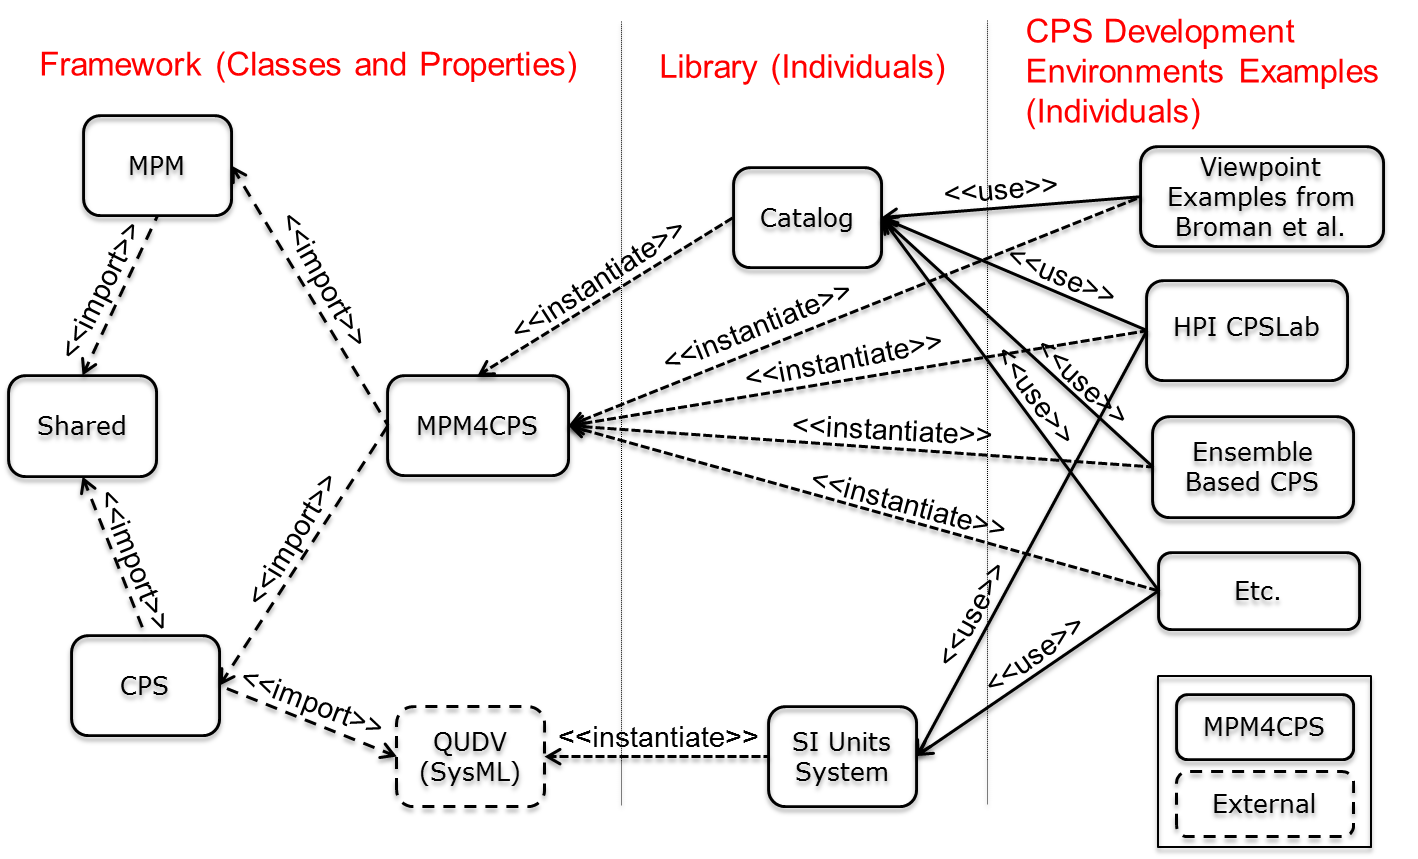
\includegraphics[width=\textwidth]{figures/ontology_structure.png}
\caption{Overview of the structure of the MPM4CPS ontology}
\label{fig:ontology_structure}
\end{figure}

In figure \ref{fig:ontology_structure}, the structure of the framework and its
elements in form of the different ontologies and its instances is  presented.

The first column depicts the framework and its ontologies as presented in this report. This includes 
the ontology of Cyber-Physical Systems presented in chapter \ref{ch:cps}, the
ontology of Multi-Paradigm Modeling presented in chapter \ref{ch:mpm} and the
combined ontology of Multi-Paradigm Modeling for Cyber-Physical Systems
presented in chapter \ref{ch:mpm4cps}.

The Glossary of Terms for Cyber-Physical Systems presented in the report on the
State-of-the-art on Current Formalisms used in Cyber-Physical Systems
Development covered by deliverable D1.1 \cite{MPM4CPS-D1-1v1} is extracted
automatically from these ontologies and the  contained concepts defining the
framework.

In the second column, the catalog of modeling languages\uidx{ModelingLanguage} and tools\uidx{Tool} that
is an instance of the MPM4CPS ontology presented  in the report on the
State-of-the-art on Current Formalisms used in Cyber-Physical Systems
Development covered by deliverable D1.1 \cite{MPM4CPS-D1-1v1} is depicted. The
catalog of that deliverable will be automatically derived from this instance
such that ontology and instances can be kept consistent with only minimal
coordination efforts.%https://www.sharelatex.com/project/5ae2fed74797f945fcb70b13

In the third column, some examples for CPS employing MPM in form of
mega models are depicted that are presented in detail in the Catalog of
Megamodel Examples in chapter \ref{ch:catalog}. As shown in the figure, these
examples employ the languages and tools listed in the report on the
State-of-the-art on Current Formalisms used in Cyber-Physical Systems
Development and covered by deliverable D1.1 \cite{MPM4CPS-D1-1v1}, and also 
instantiate the MPM4CPS ontology.

\section{Ontology Development Approach}


To define the ontologies of WG1, we have carried out a domain analysis process\uidx{Process}
\cite{Kang1990}. The domain analysis process can be defined as the process of
identifying, capturing\uidx{CapturingOperation} and organizing domain knowledge about the problem domain with the purpose of making it reusable when creating new systems. A domain is usually defined as an area of knowledge or activity characterized by a set of concepts and terminology understood by practitioners in that area. In our context, the domains of consideration are the domains of CPS and MPM, and we aim to
derive and model the concepts of these domains. Figure \ref{fig:domain_analysis_methods}
represents the common structure of domain analysis methods as it has been derived from survey studies on domain analysis methods.

\begin{figure}[!htb]
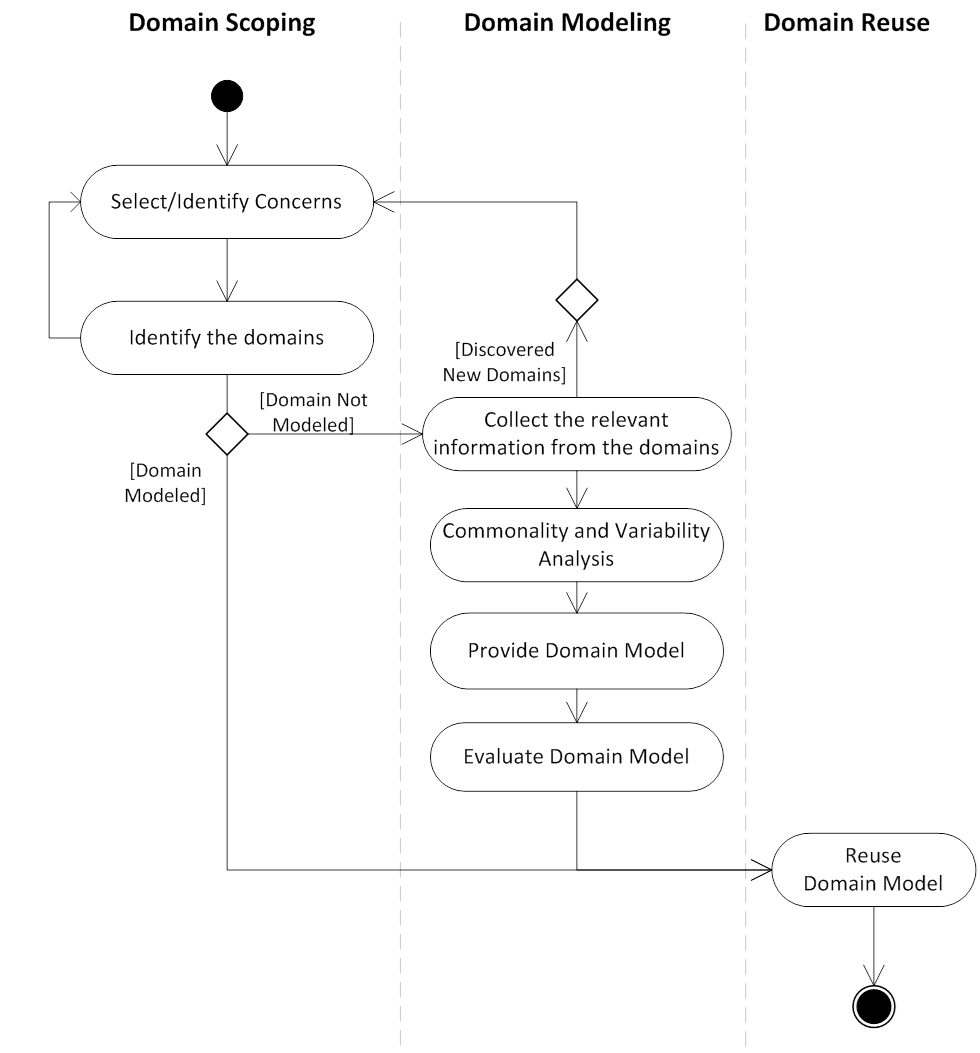
\includegraphics[width=\textwidth]{figures/domain_analysis_methods.png}
\caption{Common structure of domain analysis methods (adopted from:
\cite{Tekinerdogan2013})}
\label{fig:domain_analysis_methods}
\end{figure}

Conventional domain analysis methods consist generally of the activities Domain
Scoping  and Domain Modeling: Domain Scoping identifies the domains of
interest, the stakeholders\uidx{Stakeholder}, and their goals, and defines the scope of the
domain. Domain Modeling is the activity for representing the domain, or the
domain model. In our study the outputs of the domain modeling process\uidx{Process} will be the set of ontologies for CPS and MPM as identified by figure \ref{fig:ontology_structure}.

The domain model can be represented in different forms such as ontological
languages, object-oriented language, algebraic specifications, rules, conceptual
models etc. Typically, a domain model is formed through a commonality and
variability analysis to concepts in the domain. A domain model is used as a
basis for engineering components intended for use in multiple applications
within the domain.

One of the popular approaches for domain modeling is feature modeling. A feature
is a system property that is relevant to some stakeholder\uidx{Stakeholder} and is used to capture
commonalities or discriminate between. A feature model is a model that defines
features and their dependencies. Feature models are usually represented in
feature diagrams (or tables). A feature diagram is a tree with the root
representing a concept (e.g., a software system), and its descendent nodes are
features. Relationships between a parent feature and its child features (or
sub-features) are categorized as:

\begin{itemize}
	\item Mandatory - child feature is required.
	\item Optional - child feature is optional.
	\item Or -at least one of the sub-features must be selected.
	\item Alternative (xor) - one of the sub-features must be selected
\end{itemize}

A feature configuration is a set of features which describes a member of an SPL.
A feature constraint further restricts the possible selections of features to
define configurations.  The most common feature constraints\uidx{Constraint} are:

\begin{itemize}
	\item A requires B - The selection of A in a product implies the selection of B.
	\item A excludes B - A and B cannot be part of the same product.
\end{itemize}

Feature modeling is a domain modeling technique, which is widely used to model
the commonality and variability of a particular domain or product family.
Another domain modeling technique that is used in software engineering is
ontology modeling. A commonly accepted definition of an ontology is
``an explicit specification of conceptualization'' \cite{Gruber1995}. An
ontology represents the semantics of concepts and their relationships using some description language. Basic feature modeling is also a concept description technique that focuses on modeling both the commonality and variability. It has been indicated that feature models can be seen as views on ontologies \cite{Czarnecki2006}.

To develop the WG1 ontologies presented in details in the following chapters, the aforementioned techniques have been used. For the CPS ontology, feature modeling has been used while for the MPM ontology, modeling with the W3C OWL language and its tool Protege has been used. Consequently, using the concepts developed in \cite{Czarnecki2006}, we present a version of the CPS ontology using the W3C OWL language that has been derived directly from the feature model. This enables uniform study and analysis of all the ontologies, with same semantics, presented in this deliverable. 
%In the next year, it is planned to also integrate the CPS ontology into the Protege OWL technical space.
\chapter{Ontology of Shared Concepts}\LEAD{Holger}\ALSO{Dominique}\STATUS{started; initial comments by Holger}
\label{ch:core}
%
As outlined in the introduction of Chapter~\ref{ch:introduction} in Figure~\ref{fig:ontology_structure}, the structure of the framework and its elements are organized in the form of different ontologies providing classes for the covered domains and individuals (instances) for these classes. The ontology presented in this chapter serves in this context as foundation to define an ontology of Cyber-Physical Systems later in Chapter~\ref{ch:cps} and an ontology of Multi-Paradigm Modeling in Chapter~\ref{ch:mpm}. Then, these ontologies together with the one of this chapter are combined to define an ontology of Multi-Paradigm Modeling for Cyber-Physical Systems presented in Chapter~\ref{ch:mpm4cps}. 
%
%\DONE[DB]{ Holger 2 Dominique: NEW, please review ... DB: Done, HG: minor revision, please review ... DB: Reviewed.}

%\TODONOTE[DB]{ Holger 2 Dominique: I suggest that we present a more detailed version of the shared ontology here, as we later will have a full chapter on this. In addition, we may introduce the machinery employed for the ontology here as well in more detail (e.g., providing a short introduction into ontologies and the employed notation). What do you think? }

%\LATERNOTE{ HG: The lack of an example might be accepted for the report, but is a problem for the later planned book chapters. Maybe we can sketch here or in the examples informally the link between the examples and the core ontology. }

% ========================================================
%****************************************************************************************************************************************
% File: shared-ontology.tex
%
% This file is automatically generated. Please do not edit!
%****************************************************************************************************************************************
\section{Ontology Overview}

The shared ontology defines concepts that do not specifically pertain to the CPS and neither to the MPM domain, but that are required by one of these domains or both. It is a place to define concepts reusable by all the ontologies developed in this effort. The classes and properties provided in this ontology may be refined by other ontologies of the framework to provide specialized definitions for more specific domains. 

The shared ontology is divided into five domains for capturing concepts related to the \uidxp{linguistic}, \uidxp{workflow}, \uidxp{project management},  \uidxp{architecture} and  \uidxp{paradigm} domains. When applicable, the classes of these domains were based on well-known standards and other de-facto standard works. 
Note that these domains are not disjoint so that a class may appear under several domain concept classes.

Figure \ref{fig:shared_ontology_overview} shows an overview of the shared ontology. The details of each concept are
provided in the following subsections.

\begin{figure}[!htb]
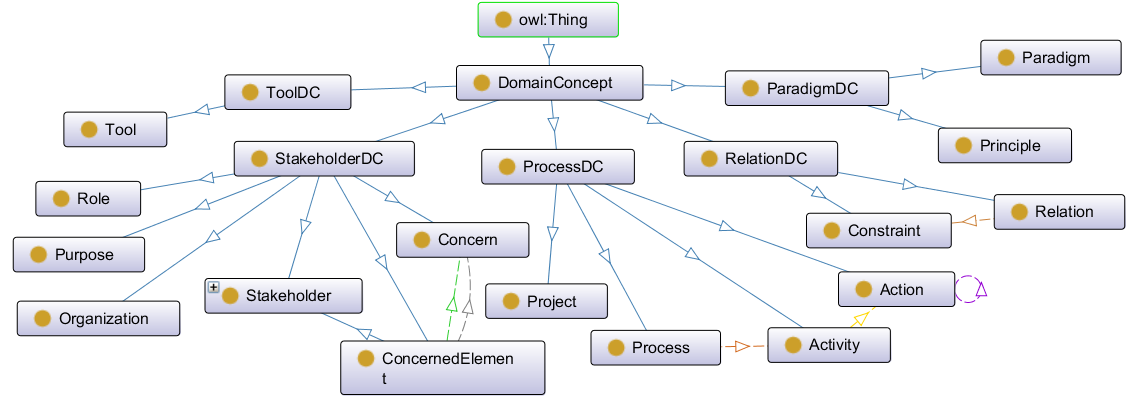
\includegraphics[width=\textwidth]{figures/shared_ontology_overview.png}
\caption{Overview of the shared ontology}
\label{fig:shared_ontology_overview}
\end{figure}

\section{DomainConcept (Domain Concepts)}
\label{sec:shared:classes}

This class groups all domain concepts of the MPM4CPS ontologies. It is further divided into  subclasses for the different sub-domains of the MPM4CPS ontologies. The classes for these sub-domains can be identified from their DC (Domain Concept) suffix. 
These sub-domain classes allow organizing the ontology into specific domains thus facilitating the navigation across the many concepts of the MPM4CPS ontologies. Note that the sub-domain classes are not disjoint from each other so that a class may belong to several sub-domain concepts.

\subsection{ArchitectureDC (Architecture Domain Concepts)}
\label{subsecDC:ArchitectureDC}

This class groups concepts that are related to the \uidxp{architecture} domain. These concepts were initially inspired from the well-known ISO/IEC/ IEEE 42010 standard and its adaptation by \cite{Broman2012}. 

The architecture is extremely vast and only a minimal subset from its concepts has been considered and adapted for the MPM4CPS sub-domains (see figure~2 of \cite{Hilliard2012}).

\subsubsection{ArchitectureDescription}
\label{subsubsecC:ArchitectureDescription}
\didx{ArchitectureDescription}

ArchitectureDescription class is en entity that expresses one architecture for one system of interest.

\textbf{Subclass of}
\begin{itemize}
	\item \textbf{ArchitectureDC} (see section \ref{subsecDC:ArchitectureDC})
\end{itemize}






\subsubsection{Concern}
\label{subsubsecC:Concern}
\didx{Concern}

In computer science, a concern is a particular set of information that has an effect on the code of a computer program. A concern can be as general as the details of database interaction or as specific as performing a primitive calculation, depending on the level of conversation between developers and the program being discussed. IBM uses the term concern space to describe the sectioning of conceptual information.

\textbf{Subclass of}
\begin{itemize}
	\item \textbf{ArchitectureDC} (see section \ref{subsecDC:ArchitectureDC})
	\item \textbf{ProjectManagementDC} (see section \ref{subsecDC:ProjectManagementDC})
\end{itemize}






\subsubsection{Stakeholder}
\label{subsubsecC:Stakeholder}
\didx{Stakeholder}

A stakeholder is an individual, group, or organization who may affect, be affected by, or perceive itself to be affected by a decision, activity, or outcome of a project.

\textbf{Subclass of}
\begin{itemize}
	\item \textbf{ArchitectureDC} (see section \ref{subsecDC:ArchitectureDC})
	\item \textbf{ProjectManagementDC} (see section \ref{subsecDC:ProjectManagementDC})
\end{itemize}


\textbf{References}
\begin{itemize}
	
\item \url{https://en.wikipedia.org/wiki/Project_stakeholder}
\end{itemize}




\subsubsection{System}
\label{subsubsecC:System}
\didx{System}

System class is a group of interacting or interrelated entities that form a unified whole.

\textbf{Subclass of}
\begin{itemize}
	\item \textbf{ArchitectureDC} (see section \ref{subsecDC:ArchitectureDC})
\end{itemize}






\subsubsection{ToolProvider}
\label{subsubsecC:ToolProvider}
\didx{ToolProvider}

Who provides the product and gives the licenses (e.g. company, university, group, ..)

\textbf{Subclass of}
\begin{itemize}
	\item \textbf{Stakeholder} (see section \ref{subsubsecC:Stakeholder})
\end{itemize}



\subsection{LinguisticDC}
\label{subsecDC:LinguisticDC}

This class groups domain concepts related to the linguistic aspects, such as modeling, programming, formal and even natural languages and their syntax.

\subsubsection{ArtificialLanguage}
\label{subsubsecC:ArtificialLanguage}
\didx{ArtificialLanguage}

ArtificialLanguage class is about the languages that can be processed by machines (computers).

\textbf{Subclass of}
\begin{itemize}
	\item \textbf{Language} (see section \ref{subsubsecC:Language})
	\item \textbf{ArtificialLanguage} (see section \ref{subsubsecC:ArtificialLanguage})
\end{itemize}






\subsubsection{Language}
\label{subsubsecC:Language}
\didx{Language}

A language is a concrete realization of a set of formalisms. A language has a set of concrete syntaxes. The language may deviate slightly from the formalisms it realizes in the semantics that it realizes, or may realize multiple
semantics.

\textbf{Subclass of}
\begin{itemize}
	\item \textbf{LinguisticDC} (see section \ref{subsecDC:LinguisticDC})
	\item \textbf{Language} (see section \ref{subsubsecC:Language})
	\item \textbf{Language} (see section \ref{subsubsecC:Language})
\end{itemize}






\subsubsection{NaturalLanguage}
\label{subsubsecC:NaturalLanguage}
\didx{NaturalLanguage}

NaturalLanguage class gathers  natural languages are those spoken by humans such as English, French, etc.

\textbf{Subclass of}
\begin{itemize}
	\item \textbf{Language} (see section \ref{subsubsecC:Language})
\end{itemize}






\subsubsection{Semantics}
\label{subsubsecC:Semantics}
\didx{Semantics}

Semantics (from Ancient Greek: ``significant'') is primarily the linguistic, and also philosophical study of meaning in language, programming languages, formal logics, and semiotics. It focuses on the relationship between signifiers-like words, phrases, signs, and symbols-and what they stand for, their denotation.

\textbf{Subclass of}
\begin{itemize}
	\item \textbf{LinguisticDC} (see section \ref{subsecDC:LinguisticDC})
\end{itemize}






\subsubsection{Syntax}
\label{subsubsecC:Syntax}
\didx{Syntax}

According to Wikipedia, a Syntax ``is the set of rules, principles, and processes that govern the structure of sentences (sentence structure) in a given language''.

\textbf{Subclass of}
\begin{itemize}
	\item \textbf{LinguisticDC} (see section \ref{subsecDC:LinguisticDC})
\end{itemize}



\subsection{ParadigmDC (Paradigm Domain Concepts)}
\label{subsecDC:ParadigmDC}

This class groups concepts that are related to the \uidxp{paradigm} domain. In this shared ontology, the paradigm domain is introduced in its broad usual sense. These concepts can be refined for the different disciplines such as modeling or programming paradigms.

\subsubsection{Characteristic}
\label{subsubsecC:Characteristic}
\didx{Characteristic}

The Characteristic class is related with  EngineeringParadigm using  the hasCharacterisics object property.

\textbf{Subclass of}
\begin{itemize}
	\item \textbf{ParadigmDC} (see section \ref{subsecDC:ParadigmDC})
\end{itemize}






\subsubsection{CharacteristicSet}
\label{subsubsecC:CharacteristicSet}
\didx{CharacteristicSet}

A set of Characteristics.

\textbf{Subclass of}
\begin{itemize}
	\item \textbf{ParadigmDC} (see section \ref{subsecDC:ParadigmDC})
\end{itemize}






\subsubsection{DecisionProcedure}
\label{subsubsecC:DecisionProcedure}
\didx{DecisionProcedure}

It must be possible to decide if an artifact satisfies a paradigmatic property. This is achieved using a set of DecisionProcedure associated with a ParadigmaticProperty via the hasDecisionProcedures object property.

\textbf{Subclass of}
\begin{itemize}
	\item \textbf{ParadigmDC} (see section \ref{subsecDC:ParadigmDC})
\end{itemize}






\subsubsection{EngineeringArtifact}
\label{subsubsecC:EngineeringArtifact}
\didx{EngineeringArtifact}

EngineeringArtifact class represents any artifact employed to engineer systems.

\textbf{Subclass of}
\begin{itemize}
	\item \textbf{ParadigmDC} (see section \ref{subsecDC:ParadigmDC})
\end{itemize}






\subsubsection{EngineeringEnvironment}
\label{subsubsecC:EngineeringEnvironment}
\didx{EngineeringEnvironment}

The EngineeringEnvironment and EngineeringArtifact classes are related to each other via the hasArtifacts object property.

\textbf{Subclass of}
\begin{itemize}
	\item \textbf{ParadigmDC} (see section \ref{subsecDC:ParadigmDC})
\end{itemize}






\subsubsection{EngineeringParadigm}
\label{subsubsecC:EngineeringParadigm}
\didx{EngineeringParadigm}

EngineeringParadigm class is a specific view of engineering environments.

\textbf{Subclass of}
\begin{itemize}
	\item \textbf{ParadigmDC} (see section \ref{subsecDC:ParadigmDC})
\end{itemize}






\subsubsection{ParadigmaticProperty}
\label{subsubsecC:ParadigmaticProperty}
\didx{ParadigmaticProperty}

Paradigm characteristics are defined by the ParadigmaticProperty class and are related to Paradigm characteristics using the hasProperties object property.

\textbf{Subclass of}
\begin{itemize}
	\item \textbf{ParadigmDC} (see section \ref{subsecDC:ParadigmDC})
\end{itemize}






\subsubsection{PropertyExpression}
\label{subsubsecC:PropertyExpression}
\didx{PropertyExpression}

A paradigmatic property is expressed as a set of PropertyExpression associated with a paradigmatic property via the hasExpressions object property.

\textbf{Subclass of}
\begin{itemize}
	\item \textbf{ParadigmDC} (see section \ref{subsecDC:ParadigmDC})
\end{itemize}



\subsection{ProjectManagementDC (Project Management Domain Concepts)}
\label{subsecDC:ProjectManagementDC}

This class groups concepts that are related to the well-known project management domain. The concepts are mostly inspired from the ISO 21500 standard and the PMI (Project Management Institute). This domain is extremely vast and only a minimal subset from the core project management doamin concepts has been considered and adapted for the MPM4CPS sub-domains.

\subsubsection{ActivityPerformer}
\label{subsubsecC:ActivityPerformer}
\didx{ActivityPerformer}

The ActivityPerformer class is  subclassed into the Participant  and the Application classes.

\textbf{Subclass of}
\begin{itemize}
	\item \textbf{Resource} (see section \ref{subsubsecC:Resource})
	\item \textbf{WorkflowDC} (see section \ref{subsecDC:WorkflowDC})
\end{itemize}






\subsubsection{Application}
\label{subsubsecC:Application}
\didx{Application}

The Application class is a description of the IT applications or interfaces which may be invoked by the service to support, or wholly automate, the processing associated with each activity.

\textbf{Subclass of}
\begin{itemize}
	\item \textbf{ActivityPerformer} (see section \ref{subsubsecC:ActivityPerformer})
\end{itemize}






\subsubsection{Concern}
\label{subsubsecC:Concern}
\didx{Concern}

In computer science, a concern is a particular set of information that has an effect on the code of a computer program. A concern can be as general as the details of database interaction or as specific as performing a primitive calculation, depending on the level of conversation between developers and the program being discussed. IBM uses the term concern space to describe the sectioning of conceptual information.

\textbf{Subclass of}
\begin{itemize}
	\item \textbf{ArchitectureDC} (see section \ref{subsecDC:ArchitectureDC})
	\item \textbf{ProjectManagementDC} (see section \ref{subsecDC:ProjectManagementDC})
\end{itemize}






\subsubsection{Human}
\label{subsubsecC:Human}
\didx{Human}

A human.

\textbf{Subclass of}
\begin{itemize}
	\item \textbf{Participant} (see section \ref{subsubsecC:Participant})
	\item \textbf{Resource} (see section \ref{subsubsecC:Resource})
\end{itemize}






\subsubsection{Organization}
\label{subsubsecC:Organization}
\didx{Organization}

A stakeholder belongs to an organization.

\textbf{Subclass of}
\begin{itemize}
	\item \textbf{ProjectManagementDC} (see section \ref{subsecDC:ProjectManagementDC})
\end{itemize}






\subsubsection{Participant}
\label{subsubsecC:Participant}
\didx{Participant}

The Participant class  is defined as a description of resources that can act as the performer of the various activities in the process definition.

\textbf{Subclass of}
\begin{itemize}
	\item \textbf{ActivityPerformer} (see section \ref{subsubsecC:ActivityPerformer})
\end{itemize}






\subsubsection{Resource}
\label{subsubsecC:Resource}
\didx{Resource}

Following the ISO 21500 standard, the Resource class is an artifacts that are employed by projects. 
Resources can be humans, facilities, equipment, materials, infrastructure and tools.

\textbf{Subclass of}
\begin{itemize}
	\item \textbf{ProjectManagementDC} (see section \ref{subsecDC:ProjectManagementDC})
\end{itemize}






\subsubsection{Stakeholder}
\label{subsubsecC:Stakeholder}
\didx{Stakeholder}

A stakeholder is an individual, group, or organization who may affect, be affected by, or perceive itself to be affected by a decision, activity, or outcome of a project.

\textbf{Subclass of}
\begin{itemize}
	\item \textbf{ArchitectureDC} (see section \ref{subsecDC:ArchitectureDC})
	\item \textbf{ProjectManagementDC} (see section \ref{subsecDC:ProjectManagementDC})
\end{itemize}


\textbf{References}
\begin{itemize}
	
\item \url{https://en.wikipedia.org/wiki/Project_stakeholder}
\end{itemize}




\subsubsection{Tool}
\label{subsubsecC:Tool}
\didx{Tool}

A tool.

\textbf{Subclass of}
\begin{itemize}
	\item \textbf{Application} (see section \ref{subsubsecC:Application})
	\item \textbf{Resource} (see section \ref{subsubsecC:Resource})
\end{itemize}






\subsubsection{ToolProvider}
\label{subsubsecC:ToolProvider}
\didx{ToolProvider}

Who provides the product and gives the licenses (e.g. company, university, group, ..)

\textbf{Subclass of}
\begin{itemize}
	\item \textbf{Stakeholder} (see section \ref{subsubsecC:Stakeholder})
\end{itemize}



\subsection{WorkflowDC}
\label{subsecDC:WorkflowDC}

A workflow standard process definition language defined by the Workflow Management Coalition (WfMC) WFMC-TC-1025 standard.

\subsubsection{Activity}
\label{subsubsecC:Activity}
\didx{Activity}

A logical, self-contained unit of work within a process.

\textbf{Subclass of}
\begin{itemize}
	\item \textbf{WorkflowDC} (see section \ref{subsecDC:WorkflowDC})
\end{itemize}






\subsubsection{ActivityPerformer}
\label{subsubsecC:ActivityPerformer}
\didx{ActivityPerformer}

The ActivityPerformer class is  subclassed into the Participant  and the Application classes.

\textbf{Subclass of}
\begin{itemize}
	\item \textbf{Resource} (see section \ref{subsubsecC:Resource})
	\item \textbf{WorkflowDC} (see section \ref{subsecDC:WorkflowDC})
\end{itemize}






\subsubsection{ActivitySet}
\label{subsubsecC:ActivitySet}
\didx{ActivitySet}

A set of Activities.

\textbf{Subclass of}
\begin{itemize}
	\item \textbf{WorkflowDC} (see section \ref{subsecDC:WorkflowDC})
\end{itemize}






\subsubsection{Application}
\label{subsubsecC:Application}
\didx{Application}

The Application class is a description of the IT applications or interfaces which may be invoked by the service to support, or wholly automate, the processing associated with each activity.

\textbf{Subclass of}
\begin{itemize}
	\item \textbf{ActivityPerformer} (see section \ref{subsubsecC:ActivityPerformer})
\end{itemize}






\subsubsection{BlockActivity}
\label{subsubsecC:BlockActivity}
\didx{BlockActivity}

A Block activity consists of an embedded subprocess represented by an ActivitySet.

\textbf{Subclass of}
\begin{itemize}
	\item \textbf{Activity} (see section \ref{subsubsecC:Activity})
\end{itemize}






\subsubsection{EngineeringMethodology}
\label{subsubsecC:EngineeringMethodology}
\didx{EngineeringMethodology}

EngineeringMethodology is a general strategy that outlines the way in which engineering is to be undertaken and identifies a set of engineering stages defining the strategy.

\textbf{Subclass of}
\begin{itemize}
	\item \textbf{WorkflowDC} (see section \ref{subsecDC:WorkflowDC})
\end{itemize}






\subsubsection{EngineeringStage}
\label{subsubsecC:EngineeringStage}
\didx{EngineeringStage}

EngineeringStage class represents a categorization of workflow processes to implement the stage of the methodology.

\textbf{Subclass of}
\begin{itemize}
	\item \textbf{WorkflowDC} (see section \ref{subsecDC:WorkflowDC})
\end{itemize}






\subsubsection{Human}
\label{subsubsecC:Human}
\didx{Human}

A human.

\textbf{Subclass of}
\begin{itemize}
	\item \textbf{Participant} (see section \ref{subsubsecC:Participant})
	\item \textbf{Resource} (see section \ref{subsubsecC:Resource})
\end{itemize}






\subsubsection{Participant}
\label{subsubsecC:Participant}
\didx{Participant}

The Participant class  is defined as a description of resources that can act as the performer of the various activities in the process definition.

\textbf{Subclass of}
\begin{itemize}
	\item \textbf{ActivityPerformer} (see section \ref{subsubsecC:ActivityPerformer})
\end{itemize}






\subsubsection{Process}
\label{subsubsecC:Process}
\didx{Process}

An entity providing contextual information applying to other entities within the process.

\textbf{Subclass of}
\begin{itemize}
	\item \textbf{WorkflowDC} (see section \ref{subsecDC:WorkflowDC})
\end{itemize}






\subsubsection{Route}
\label{subsubsecC:Route}
\didx{Route}

A Route is an activity that performs no work processing (and therefore has no associated resource or applications), but simply supports routing decisions among the incoming transitions and/or among the outgoing transitions.

\textbf{Subclass of}
\begin{itemize}
	\item \textbf{Activity} (see section \ref{subsubsecC:Activity})
\end{itemize}






\subsubsection{SubFlow}
\label{subsubsecC:SubFlow}
\didx{SubFlow}

A SubFlow activity is a link to the execution of an independent subprocess declared in a process package. A hasSubProcess object property is defined to link a subflow activity to its process.

\textbf{Subclass of}
\begin{itemize}
	\item \textbf{Activity} (see section \ref{subsubsecC:Activity})
\end{itemize}






\subsubsection{Tool}
\label{subsubsecC:Tool}
\didx{Tool}

A tool.

\textbf{Subclass of}
\begin{itemize}
	\item \textbf{Application} (see section \ref{subsubsecC:Application})
	\item \textbf{Resource} (see section \ref{subsubsecC:Resource})
\end{itemize}






\subsubsection{Transition}
\label{subsubsecC:Transition}
\didx{Transition}

A Transition relates an activity via the from and to references to another activity to be executed if a condition defined by the transition is satisfied, or if no condition is set on the transition. This determines the execution order of
the activities in the ActivitySet.

\textbf{Subclass of}
\begin{itemize}
	\item \textbf{WorkflowDC} (see section \ref{subsecDC:WorkflowDC})
\end{itemize}

\section{Properties}
\label{sec:shared:properties}


\subsection{hasActivities}
\label{subsecP:hasActivities}
Represents the \uidxp{activity}(ies) that a \uidxp{process} may use through its \uidxp{workflow}(s).

Subproperty of:
None


Domains:
\begin{itemize}
	\item \textbf{Process} (see section \ref{subsubsecC:Process})
\end{itemize}


Ranges:
\begin{itemize}
	\item \textbf{Activity} (see section \ref{subsubsecC:Activity})
\end{itemize}




\subsection{hasActivityPerformer}
\label{subsecP:hasActivityPerformer}
The hasActivityPerformer object property  relates the Activity class to the ActivityPerformer class.

Subproperty of:
None


Domains:
\begin{itemize}
	\item \textbf{Activity} (see section \ref{subsubsecC:Activity})
\end{itemize}


Ranges:
\begin{itemize}
	\item \textbf{ActivityPerformer} (see section \ref{subsubsecC:ActivityPerformer})
\end{itemize}




\subsection{hasActivitySet}
\label{subsecP:hasActivitySet}
A Block activity consists of an embedded subprocess represented by an ActivitySet. A hasActivitySet object property is defined to link a Block to its ActivitySet.

Subproperty of:
None


Domains:
\begin{itemize}
	\item \textbf{BlockActivity} (see section \ref{subsubsecC:BlockActivity})
\end{itemize}


Ranges:
\begin{itemize}
	\item \textbf{ActivitySet} (see section \ref{subsubsecC:ActivitySet})
\end{itemize}




\subsection{hasArchitecture}
\label{subsecP:hasArchitecture}
The hasArchitecture object property is defined to relate a system to its architecture.

Subproperty of:
None


Domains:
\begin{itemize}
	\item \textbf{System} (see section \ref{subsubsecC:System})
\end{itemize}


Ranges:
None




\subsection{hasArtifacts}
\label{subsecP:hasArtifacts}
The hasArtifacts object property allows to relate the EngineeringEnvironment and EngineeringArtifact classes.

Subproperty of:
None


Domains:
\begin{itemize}
	\item \textbf{EngineeringEnvironment} (see section \ref{subsubsecC:EngineeringEnvironment})
\end{itemize}


Ranges:
\begin{itemize}
	\item \textbf{EngineeringArtifact} (see section \ref{subsubsecC:EngineeringArtifact})
\end{itemize}




\subsection{hasCharacteristics}
\label{subsecP:hasCharacteristics}
The hasCharacteristics allows to relate the EngineeringParadigm class to Characteristics class.

Subproperty of:
None


Domains:
\begin{itemize}
	\item \textbf{EngineeringParadigm} (see section \ref{subsubsecC:EngineeringParadigm})
\end{itemize}


Ranges:
\begin{itemize}
	\item \textbf{Characteristic} (see section \ref{subsubsecC:Characteristic})
\end{itemize}




\subsection{hasContainedActivitySet}
\label{subsecP:hasContainedActivitySet}
The hasContainedActivitySet property allows to relate the Process with the ActivitySet(s) associated with it.

Subproperty of:
None


Domains:
\begin{itemize}
	\item \textbf{Process} (see section \ref{subsubsecC:Process})
\end{itemize}


Ranges:
\begin{itemize}
	\item \textbf{ActivitySet} (see section \ref{subsubsecC:ActivitySet})
\end{itemize}




\subsection{hasDecisionProcedures}
\label{subsecP:hasDecisionProcedures}
It must be possible to decide if an artifact satisfies a paradigmatic property.  
This is achieved using a set of DecisionProcedure associated with a ParadigmaticProperty via the hasDecisionProcedures object property.

Subproperty of:
None


Domains:
\begin{itemize}
	\item \textbf{ParadigmaticProperty} (see section \ref{subsubsecC:ParadigmaticProperty})
\end{itemize}


Ranges:
\begin{itemize}
	\item \textbf{DecisionProcedure} (see section \ref{subsubsecC:DecisionProcedure})
\end{itemize}




\subsection{hasExpressedArchitecture}
\label{subsecP:hasExpressedArchitecture}
The ArchitectureDescription class is an entity that expresses one architecture for one system of interest. 
Those classes are related with the hasIdentifiedSystem and hasExpressedArchitecture object properties.

Subproperty of:
None


Domains:
\begin{itemize}
	\item \textbf{ArchitectureDescription} (see section \ref{subsubsecC:ArchitectureDescription})
\end{itemize}


Ranges:
None




\subsection{hasExpressions}
\label{subsecP:hasExpressions}
A paradigmatic property is expressed as a set of PropertyExpression associated with a paradigmatic property via the hasExpressions object property.

Subproperty of:
None


Domains:
\begin{itemize}
	\item \textbf{ParadigmaticProperty} (see section \ref{subsubsecC:ParadigmaticProperty})
\end{itemize}


Ranges:
\begin{itemize}
	\item \textbf{PropertyExpression} (see section \ref{subsubsecC:PropertyExpression})
\end{itemize}




\subsection{hasIdentifiedConcern}
\label{subsecP:hasIdentifiedConcern}
An architecture description  identifies the concerns of stackeholders  via the hasIdentifiedConcern object properties.

Subproperty of:
None


Domains:
\begin{itemize}
	\item \textbf{ArchitectureDescription} (see section \ref{subsubsecC:ArchitectureDescription})
\end{itemize}


Ranges:
\begin{itemize}
	\item \textbf{Concern} (see section \ref{subsubsecC:Concern})
\end{itemize}




\subsection{hasIdentifiedStakeholder}
\label{subsecP:hasIdentifiedStakeholder}
An architecture description  identifies stakeholders via the hasIdentifiedStakeholder object properties.

Subproperty of:
None


Domains:
\begin{itemize}
	\item \textbf{ArchitectureDescription} (see section \ref{subsubsecC:ArchitectureDescription})
\end{itemize}


Ranges:
\begin{itemize}
	\item \textbf{Stakeholder} (see section \ref{subsubsecC:Stakeholder})
\end{itemize}




\subsection{hasIdentifiedSystem}
\label{subsecP:hasIdentifiedSystem}
The ArchitectureDescription class is an entity that expresses one architecture for one system of interest. 
Those classes are related with the hasIdentifiedSystem and hasExpressedArchitecture object properties.

Subproperty of:
None


Domains:
\begin{itemize}
	\item \textbf{ArchitectureDescription} (see section \ref{subsubsecC:ArchitectureDescription})
\end{itemize}


Ranges:
\begin{itemize}
	\item \textbf{System} (see section \ref{subsubsecC:System})
\end{itemize}




\subsection{hasNextStage}
\label{subsecP:hasNextStage}
The hasNextStage object property relates methodology stages in case the stages must be ordered.

Subproperty of:
None


Domains:
\begin{itemize}
	\item \textbf{EngineeringStage} (see section \ref{subsubsecC:EngineeringStage})
\end{itemize}


Ranges:
\begin{itemize}
	\item \textbf{EngineeringStage} (see section \ref{subsubsecC:EngineeringStage})
\end{itemize}




\subsection{hasProperties}
\label{subsecP:hasProperties}
Paradigm characteristics are defined by the ParadigmaticProperty class and related to Paradigm characteristics using the hasProperties object property.

Subproperty of:
None


Domains:
\begin{itemize}
	\item \textbf{EngineeringParadigm} (see section \ref{subsubsecC:EngineeringParadigm})
\end{itemize}


Ranges:
\begin{itemize}
	\item \textbf{ParadigmaticProperty} (see section \ref{subsubsecC:ParadigmaticProperty})
\end{itemize}




\subsection{hasProvider}
\label{subsecP:hasProvider}
The company/university which the tool is developed by.

Subproperty of:
None


Domains:
\begin{itemize}
	\item \textbf{Tool} (see section \ref{subsubsecC:Tool})
\end{itemize}


Ranges:
\begin{itemize}
	\item \textbf{ToolProvider} (see section \ref{subsubsecC:ToolProvider})
\end{itemize}




\subsection{hasSemantics}
\label{subsecP:hasSemantics}
The hasSemantics object property  relates a Language with its Semantics.

Subproperty of:
None


Domains:
\begin{itemize}
	\item \textbf{Language} (see section \ref{subsubsecC:Language})
\end{itemize}


Ranges:
\begin{itemize}
	\item \textbf{Semantics} (see section \ref{subsubsecC:Semantics})
\end{itemize}




\subsection{hasSetActivities}
\label{subsecP:hasSetActivities}
An ActivitySet contains a set of other activities and Transition elements declared via the hasSetActivities and hasTransitions object properties.

Subproperty of:
None


Domains:
\begin{itemize}
	\item \textbf{ActivitySet} (see section \ref{subsubsecC:ActivitySet})
\end{itemize}


Ranges:
\begin{itemize}
	\item \textbf{Activity} (see section \ref{subsubsecC:Activity})
\end{itemize}




\subsection{hasStage}
\label{subsecP:hasStage}
The EngineeringStage class represents a categorization of workflow processes to implement the stage of the methodology
using the hasStages object property.

Subproperty of:
None


Domains:
\begin{itemize}
	\item \textbf{EngineeringMethodology} (see section \ref{subsubsecC:EngineeringMethodology})
\end{itemize}


Ranges:
\begin{itemize}
	\item \textbf{EngineeringStage} (see section \ref{subsubsecC:EngineeringStage})
\end{itemize}




\subsection{hasSubProcess}
\label{subsecP:hasSubProcess}
The hasSubProcess object property links a subflow activity to its process.

Subproperty of:
None


Domains:
\begin{itemize}
	\item \textbf{SubFlow} (see section \ref{subsubsecC:SubFlow})
\end{itemize}


Ranges:
\begin{itemize}
	\item \textbf{Process} (see section \ref{subsubsecC:Process})
\end{itemize}




\subsection{hasSyntax}
\label{subsecP:hasSyntax}
Every language (natural or artificial) must have at least one syntax using the hasSyntax object property to express sentences of the language to communicate with
other entities.

Subproperty of:
None


Domains:
\begin{itemize}
	\item \textbf{Language} (see section \ref{subsubsecC:Language})
\end{itemize}


Ranges:
\begin{itemize}
	\item \textbf{Syntax} (see section \ref{subsubsecC:Syntax})
\end{itemize}




\subsection{isImplementingMethodology}
\label{subsecP:isImplementingMethodology}
A methodology is implemented by an overall workflow process defining activities supporting each stage of the methodology. 
The object property isImplementingMethodology  relates a process to the methodology it implements.

Subproperty of:
None


Domains:
\begin{itemize}
	\item \textbf{Process} (see section \ref{subsubsecC:Process})
\end{itemize}


Ranges:
\begin{itemize}
	\item \textbf{EngineeringMethodology} (see section \ref{subsubsecC:EngineeringMethodology})
\end{itemize}




\subsection{isImplementingStage}
\label{subsecP:isImplementingStage}
The isImplementingStage is defined to relate an activity to a stage it implements.

Subproperty of:
None


Domains:
\begin{itemize}
	\item \textbf{Activity} (see section \ref{subsubsecC:Activity})
\end{itemize}


Ranges:
\begin{itemize}
	\item \textbf{EngineeringStage} (see section \ref{subsubsecC:EngineeringStage})
\end{itemize}




\subsection{isTransitionFrom}
\label{subsecP:isTransitionFrom}
A Transition determines the order of execution of activities in the ActivitySet. The isTransitionFrom property allows to relate the Transition with the Activity that is being transitioned from, that results in the conditions defined by the transition being met.

Subproperty of:
None


Domains:
\begin{itemize}
	\item \textbf{Transition} (see section \ref{subsubsecC:Transition})
\end{itemize}


Ranges:
\begin{itemize}
	\item \textbf{Activity} (see section \ref{subsubsecC:Activity})
\end{itemize}




\subsection{isTransitionTo}
\label{subsecP:isTransitionTo}
A Transition determines the order of execution of activities in the ActivitySet. The isTransitionTo property allows to relate the Transition with the Activity that is being transitioned to, i.e. the Activity that is performed as a result of the execution of the Transition.

Subproperty of:
None


Domains:
\begin{itemize}
	\item \textbf{Transition} (see section \ref{subsubsecC:Transition})
\end{itemize}


Ranges:
\begin{itemize}
	\item \textbf{Activity} (see section \ref{subsubsecC:Activity})
\end{itemize}







% ========================================================
\chapter{Ontology of Cyber-Physical Systems}
\label{ch:cps}

\section{State-of-the-art}

Cyber-Physical Systems (CPS) are systems\uidx{System} that tightly integrate computation 
with networking and physical processes. Such systems form large networks that 
communicate with each other and rely on actuators and sensors to monitor and 
control complex with physical processes, creating complex feedback loops 
between the physical and the cyber worlds. CPS bring innovation in terms of 
economic and societal impacts for various kinds of industries, creating 
entirely new markets and platforms for growth. CPS have growing applications in 
various domains, including healthcare, transportation, precision agriculture, energy
conservation, environmental control, avionics, critical infrastructure control
(electric and nuclear power plants, water resources, and communications systems), 
high confidence medical devices and systems, traffic control and safety\uidx{Safety}, 
advanced automotive systems, process control, distributed robotics (telepresence, 
telemedicine), manufacturing, and smart city engineering. The positive economic 
impact of any one of these applications areas is enormous.

Technically, CPS systems are inherently heterogeneous\uidx{Heterogeneity}, typically comprising 
mechanical, hydraulic, material, electrical, electronic, and computational components. 
The engineering process\uidx{Process} of CPS requires distinct disciplines to be employed, 
resulting in a collection of models that are expressed using correspondingly 
distinct modelling formalisms\uidx{Formalism}. 

An important realization is that distinct models need to be weaved together consistently to form a complete representation of a system that enables, among other global aspects, performance analysis, exhaustive simulation and verification, hardware in the loop simulation, determining best overall parameters of the system, prototyping, or implementation. 
A new framework is required that is able to represent these connections between models and, moreover, enable reasoning about them. No single formalism is able to model all aspects of a system; modelling of a CPS system is inherently multi-paradigm\uidx{Paradigm}, which calls for a trans-disciplinary approach to be able to conjoin abstractions and models from different worlds. Physically, CPS systems are inherently heterogeneous\uidx{Heterogeneity}, typically comprising 
mechanical, hydraulic, material, electrical, electronic, among others. Those areas correspond to engineering disciplines with their own models and abstractions designed to best capture the dynamics of physical processes (e.g., differential equations, stochastic processes, etc.). Computationally, CPS systems leverage the half-century old knowledge in computer science and software engineering to essentially capture how data is transformed into other useful data, abstracting away from core physical properties occurring in the real world, and particularly the passage of time in physical processes. 

The key challenge, as identified a decade ago, is then to provide mathematical and technical foundations to conjoin physical abstractions that describe the dynamics of nature in various engineering domains, as described earlier, with models focusing solely on data transformation\uidx{TransformationOperation}. This is necessary to adequately capture and bridge both aspects of a complex, realistic cyber-physical system, and become able to reason and explore system designs collaboratively, allocating responsibilities to software and physical elements, and analyzing trade-offs between them. 

Currently, there is a few common design and modelling approaches that allow engineers to handle both aspects of CPS, allowing to bridge the involved disciplines into a shared, common one. Among the existing ones, \emph{co-simulation} showed that it is possible for computation and physics engineers to cooperate efficiently without enforcing new tools or design methods. 



\section{Ontology Overview}\label{sec:Ontology-CPS}

After a domain analysis to CPS we have derived the feature model, the top-level classification for which is shown in
figure \ref{fig:feature_model_cps_top}. The different components\uidx{Component} of a CPS system can be designed together or
separately: in the latter case, the various different components need to be integrated. A CPS has different component types which can be computational or physical. Furthermore, a CPS has a network which can have different configurations and protocols.
The various components that constitute the CPS fall under the ConstituentElement class. The subset of the feature model corresponding to the ConstituentElement class is depicted in figure \ref{fig:feature_model_cps_constituent}.
\begin{figure}[!htb]
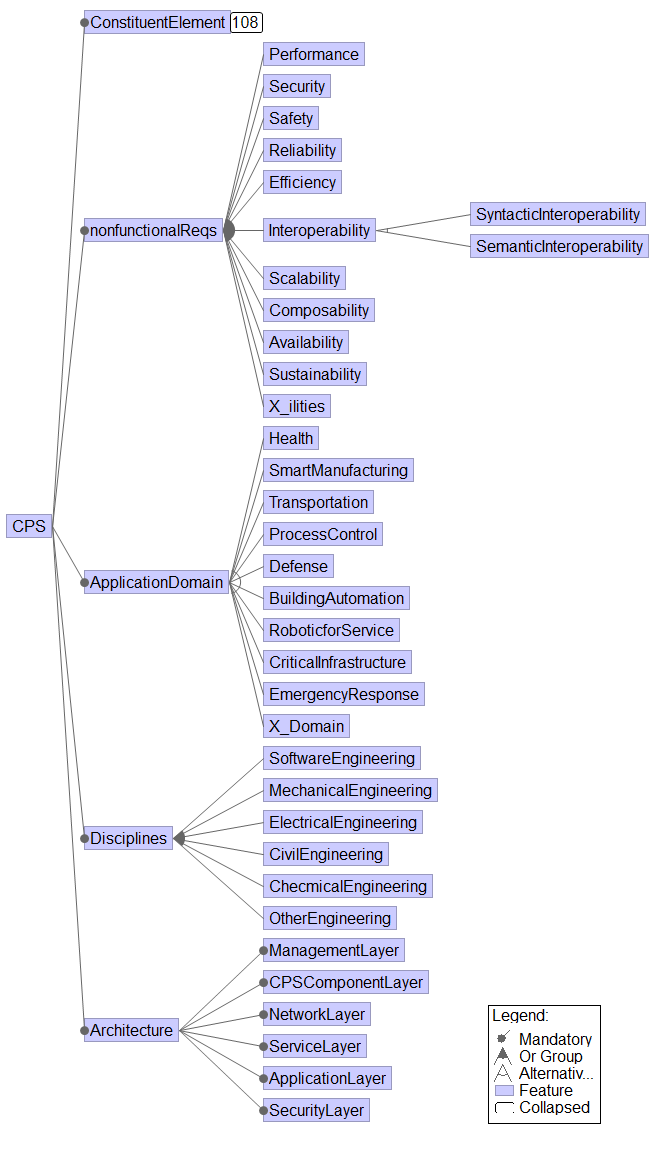
\includegraphics[width=0.42\textwidth]{figures/cps-ontology-top.png}  % STKLIK: fixing path, to make compatible with downloaded version
% 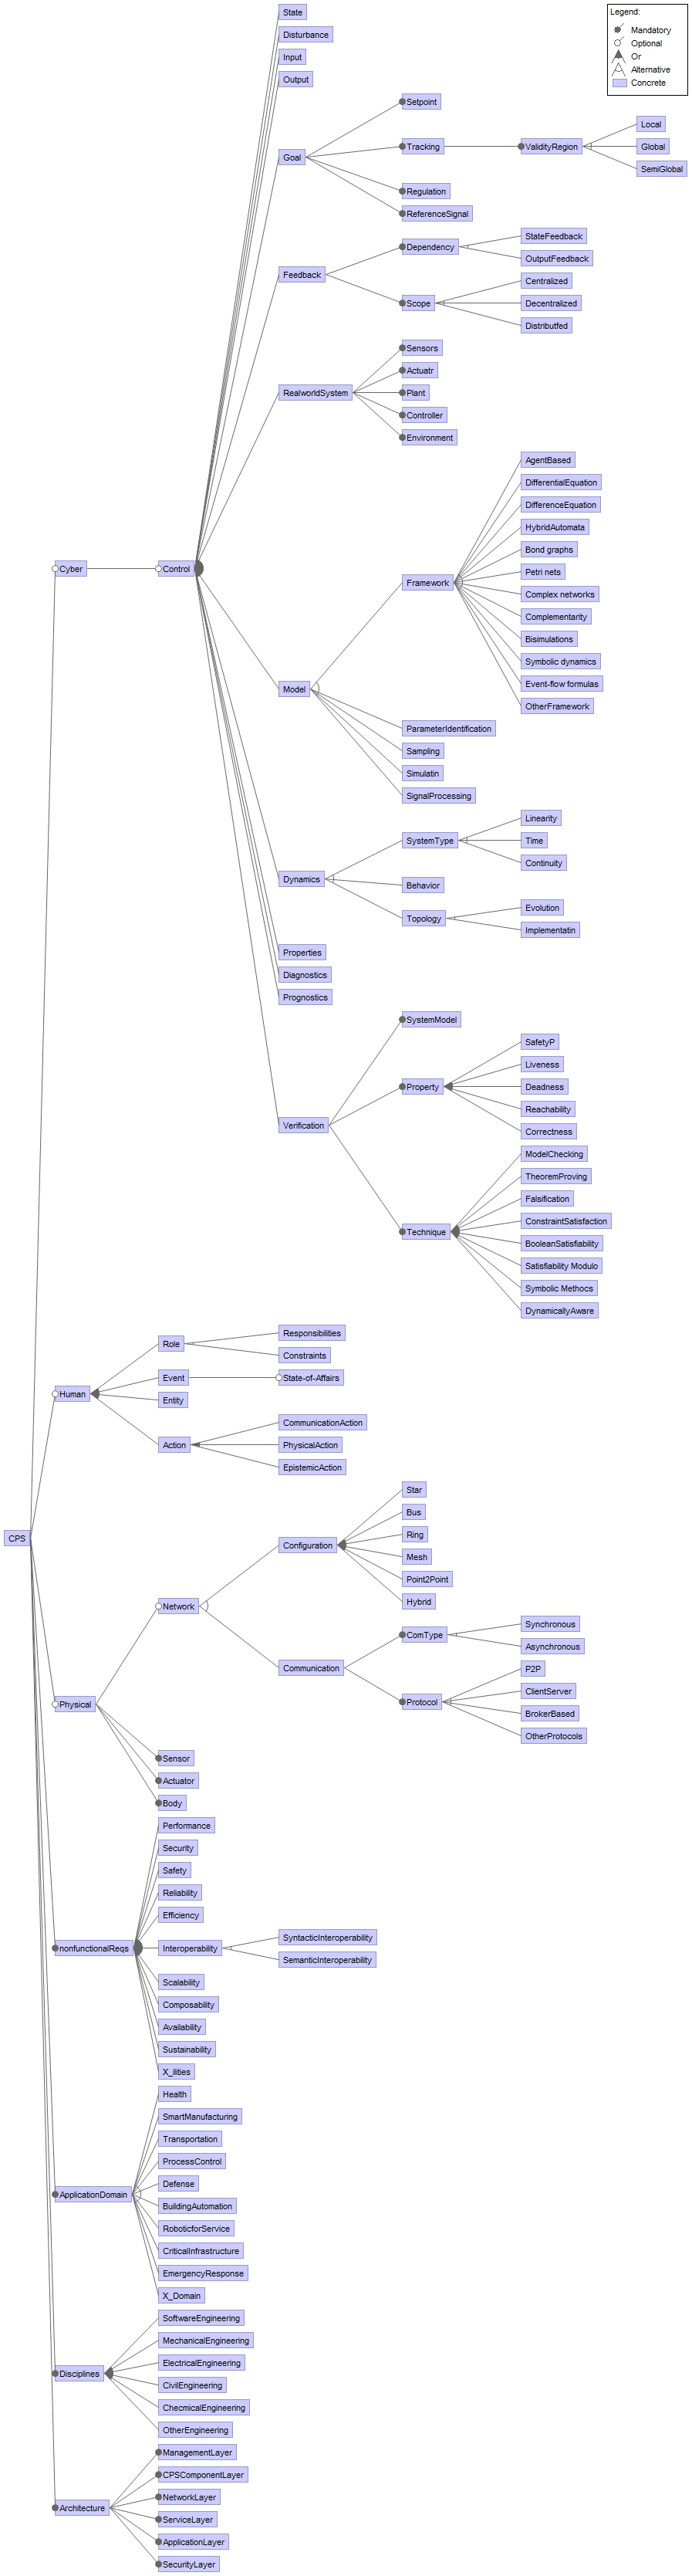
\includegraphics[width=0.42\textwidth]{fw_combine_modeling_languages/figures/cps-ontology.png}
\caption{Feature Model of a CPS representing common and variant properties}
\label{fig:feature_model_cps_top}
\end{figure}

\begin{figure}[!htb]
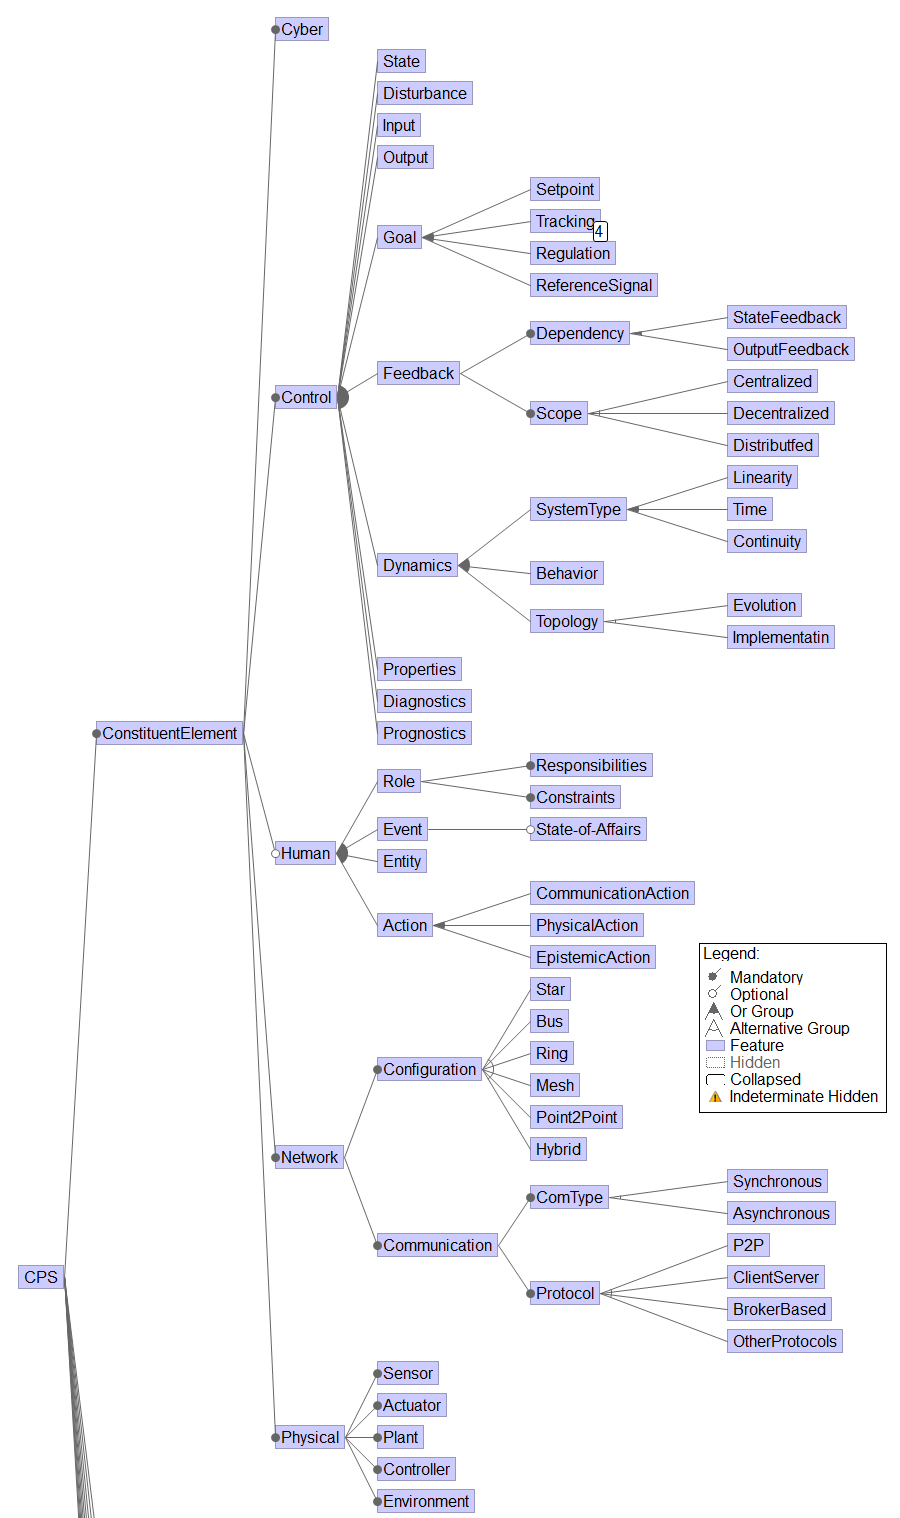
\includegraphics[width=0.42\textwidth]{figures/cps-ontology-constituent.png}  % STKLIK: fixing path, to make compatible with downloaded version
% 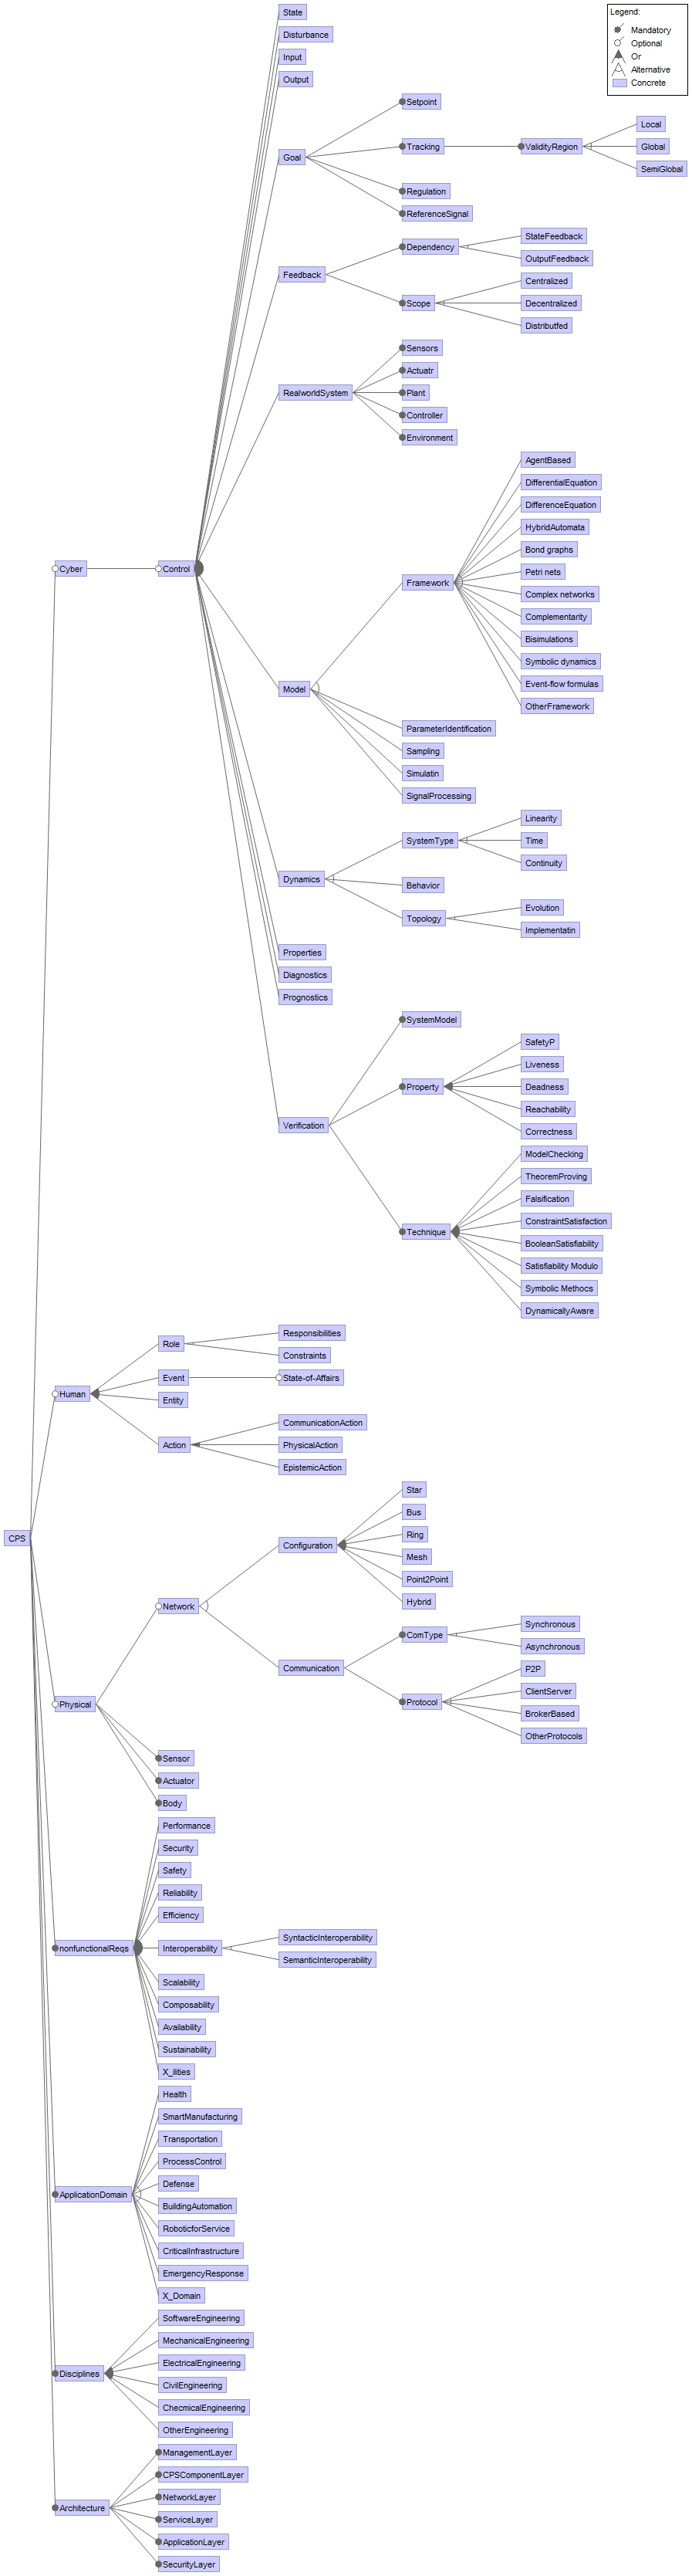
\includegraphics[width=0.42\textwidth]{fw_combine_modeling_languages/figures/cps-ontology.png}
\caption{Feature Model of a CPS representing common and variant properties}
\label{fig:feature_model_cps_constituent}
\end{figure}


%%%%%%%%%%%%%%%%%%%%%%%%%%%%%%%%%%%%%%%%%%%%%%%%%%%%%%%%%%%%%%%%%%%%%%%%%%%%%%%%%%%%%%%%%%%%%%%%%%%
% CPS 
%%%%%%%%%%%%%%%%%%%%%%%%%%%%%%%%%%%%%%%%%%%%%%%%%%%%%%%%%%%%%%%%%%%%%%%%%%%%%%%%%%%%%%%%%%%%%%%%%%%

%%%%%%%%%%%%%%%%%%%%%%%%%%%%%%%%%
% Elements
\newcommand{\CPSCyberPart}{\p{Cyber}\xspace}
\newcommand{\CPSPhysicalPart}{\p{Physical}\xspace}

%\TODOINLINE[DB]{ HG: \p{CyberPart} and \p{PhysicalPart} as used in the CPSLab text later to link to this ontology, but these elements or parts are no longer present as such are now named \CPSCyberPart and \CPSPhysicalPart without the \p{Part}. Is that OK or should we add Part? }

%\iidxp{Interoperability} relates to how well the different components\uidx{Component} can operate
%together. Here we can have syntactic or semantic interoperability. Since both
%are required in CPS, these two features are considered mandatory, rather than
%alternative. Different components in a CPS can be of the same type or of different types, thereby distinguishing between homogeneous or heterogeneous CPS. The
%final feature in the feature model presents the various application domains\uidx{ApplicationDomain} in
%which CPS can be applied including manufacturing, healthcare, transportation
%etc.

\subsection{Ontology Diagram}

In this section we describe the metamodel for
CPS which represents the concepts and their relations\uidx{Relation}. The metamodel is shown in figure \ref{fig:cps_classes}. A
CPS system consists of CPS Components\uidx{Component} that interact by using one or more Communication Protocols running on a Communication Network\uidx{Communication}. CPS Components interact with other components. A CPS Component is a Cyber Component or Physical Component. A Cyber component is a Software Component that can have various kinds of user interfaces. The Physical Component can be a Mechanical Component or Hardware Component that can include zero or more Sensors and Actuators. Sensors monitor the Physical Component while Actuators can drive them. Essentially, sensors take a
mechanical, optical, magnetic or thermal signal and convert it into voltage
and current. This provided data can then be processed and used to define the
required action\uidx{Action}. Both cyber components and physical components could
have a virtual surrogate. Virtual entities can have different representations
such as 3D models, avatars, objects or even a social network account. Some
Virtual Entities can also interact with other Virtual Entities to fulfill their
goal.

\begin{figure}[!htb]
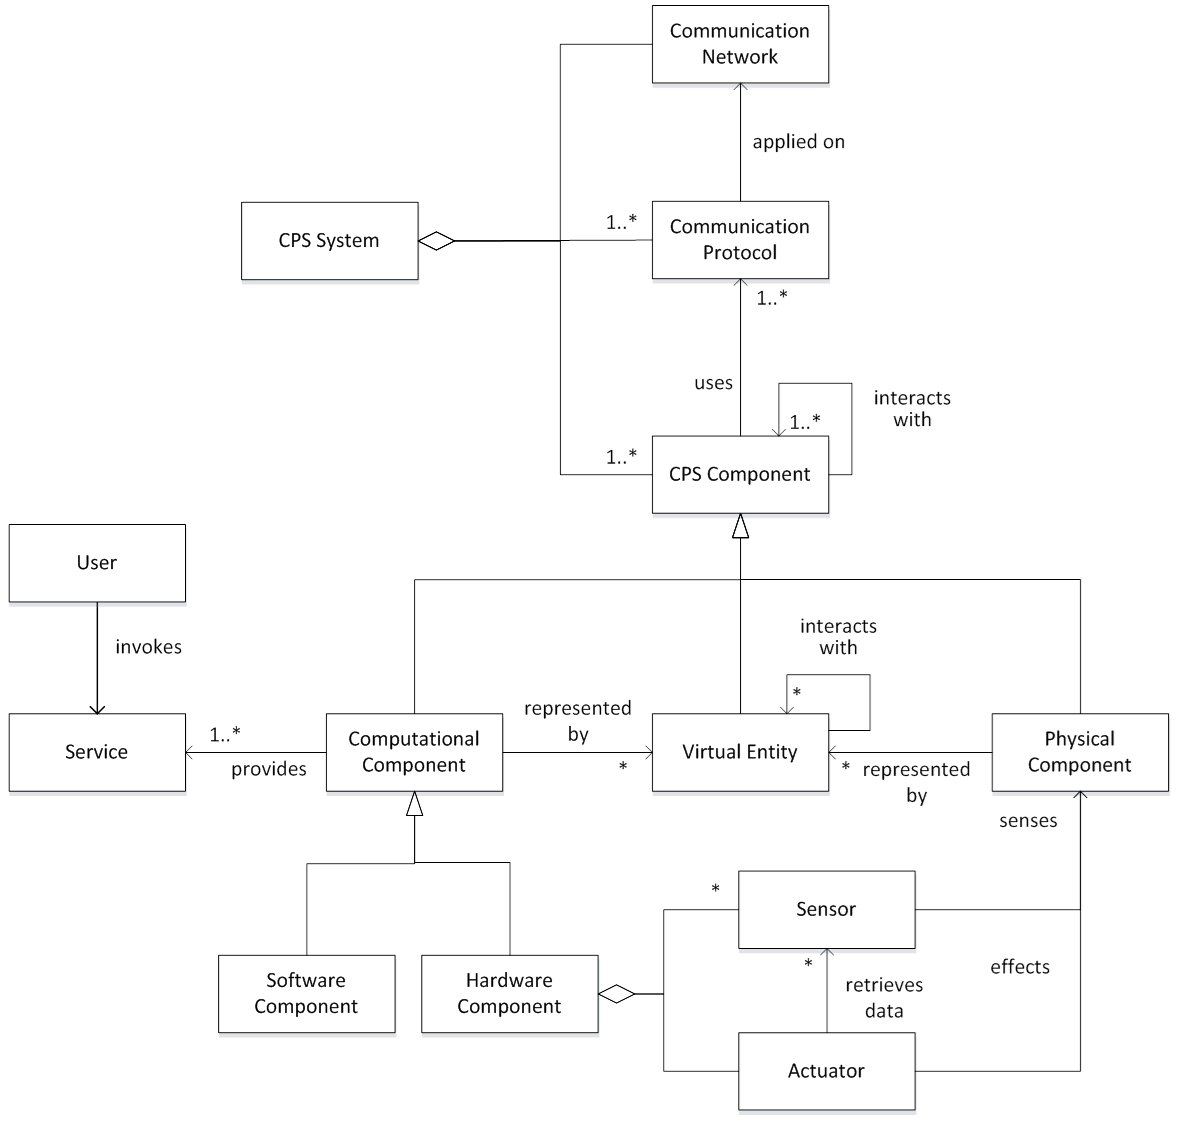
\includegraphics[width=\textwidth]{figures/cps_classes.png}
\caption{Basic concepts of CPS}
\label{fig:cps_classes}
\end{figure}

\subsection{Architecture}
The architecture\iidx{Architecture} of a CPS represents the gross level structure\uidx{Structural} of the system
consisting of cyber-physical components\uidx{Component}. Current architecture design approaches for CPS seem to be primarily  domain-specific and no standard reference architecture has been yet agreed upon. 
In this line, the development of an ontology for CPS also contributes to the efforts for designing a reference architecture. 

A CPS reference architecture defines the generic structure\uidx{Structural} of CPS architectures\uidx{Architecture} for particular application domains\uidx{ApplicationDomain}, laying the foundation for functionality, dependability\uidx{Dependability}, and other quality properties. An architecture organizes the functionality and the properties\uidx{Property} of a system to enable partitioning\uidx{SystemPart}, verification, and management. 

Figure \ref{fig:layered_cps_architecture} presents a
layered view\uidx{View} of a CPS architecture inspired on the IoT stack that arranges a CPS into successive layers of cohesive modules that share similar concerns\uidx{Concern}. The four layers at the center include device layer, network layer, CPS layer, application layer, and business layer. The CPS component\uidx{Component} layer includes the capabilities for the CPS components to undertake sensing and actuation. The network layer provides functionality for networking connectivity and transport capabilities enabling the coordination of components. The Services layer consists of functionality for generic support services (such as
data processing or data storage), and specific support capabilities for the particular applications that may already apply a degree of intelligence. The application layer orchestrates the services to provide emergent properties. Then, there are two main cross-cutting concerns\uidx{Concern}. A Security layer captures the security\uidx{Security} functionality, while the management layer supports capabilities such as device management, traffic and congestion management.


\begin{figure}[!htb]
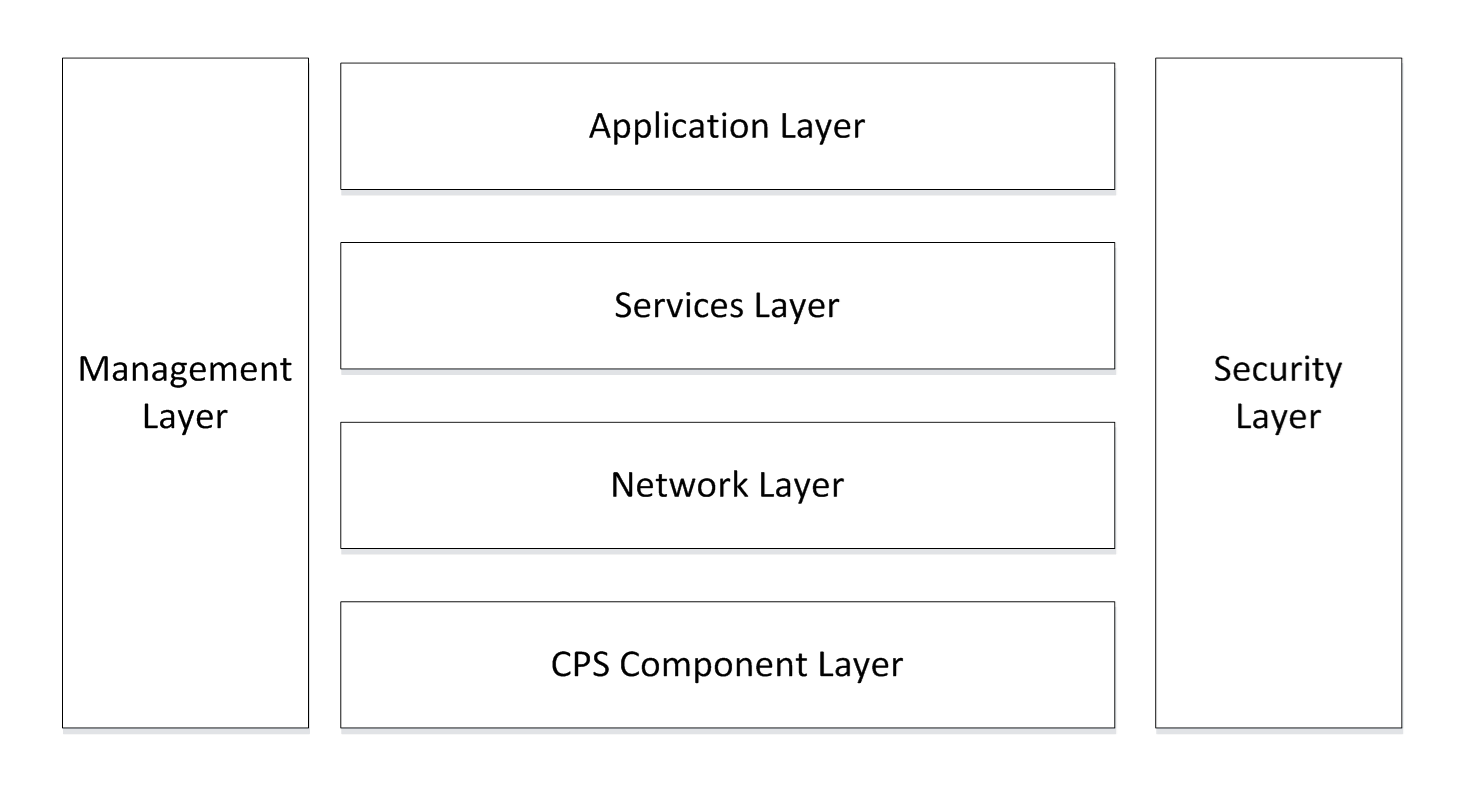
\includegraphics[width=\textwidth]{figures/layered_cps_architecture.png}
\caption{Layered view for CPS architectures\uidx{Architecture}}
\label{fig:layered_cps_architecture}
\end{figure}

The reference architecture can be used to derive concrete application
architectures. A concrete architecture defines the boundaries and constraints
for the implementation and is used to analyze risks, balance trade-offs, plan
the implementation project and allocate tasks. 

%TOTO: Ask Bedir for the missing figureThe relation between the CPS
%reference architecture and the concrete architectures is shown %in figure TODO
%missing figure?.

%****************************************************************************************************************************************
% File: cps-ontology.tex
%
% This file is automatically generated. Please do not edit!
%****************************************************************************************************************************************
\section{Ontology Overview}

\todoAuthors{Provide ``rdfs:comment'' annotation in ontology}

Figure \ref{fig:cps_ontology_overview} shows an overview of the CPS ontology. The details of each concept are
provided in the following subsections.

\begin{figure}[!htb]
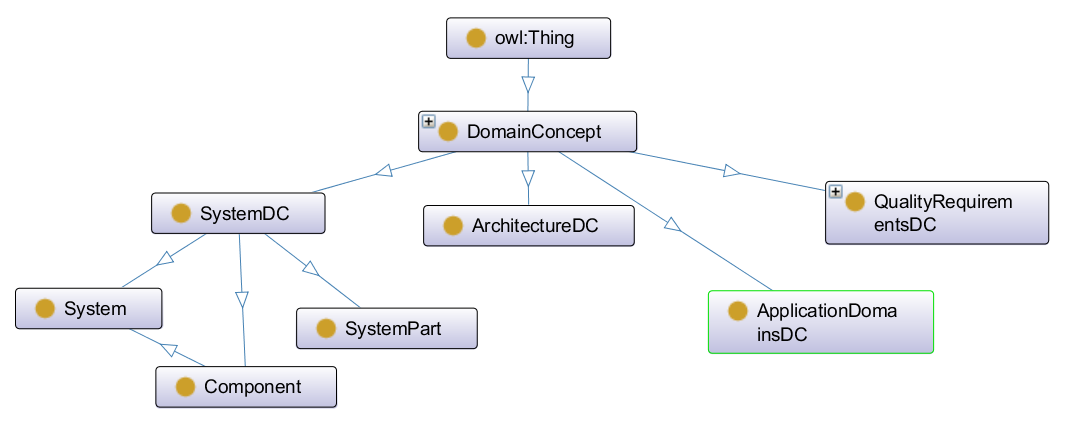
\includegraphics[width=\textwidth]{figures/cps_ontology_overview.png}
\caption{Overview of the CPS ontology}
\label{fig:cps_ontology_overview}
\end{figure}


	
\section{Domain Concepts}

This ontology of cyber-physical systems contains concepts divided into sub-domains as presented in the following subsections.

\subsection{ApplicationDomainsDC}
\label{subsecDC:ApplicationDomainsDC}

Various studies have addressed the domains and domain specific applications of CPS. Gunes et al. summarize a number of research efforts that address some of those domains, namely Smart Manufacturing, Emergency Response, Air Transportation, Critical Infrastructure, Health Care and Medicine, Intelligent Transportation, and Robotic for Service.

\subsubsection{ApplicationDomain}
\label{subsubsecC:ApplicationDomain}
\didx{ApplicationDomain}

\todoAuthors{Provide ``rdfs:comment'' annotation in ontology}

\textbf{Subclass of}
\begin{itemize}
	\item \textbf{ApplicationDomainsDC} (see section \ref{subsecDC:ApplicationDomainsDC})
\end{itemize}



\subsection{ArchitectureDC}
\label{subsecDC:ArchitectureDC}

\todoAuthors{Provide ``rdfs:comment'' annotation in ontology}





\subsection{QualityRequirementsDC}
\label{subsecDC:QualityRequirementsDC}

Cyber-Physical Systems revolutionize our interaction with the physical world. Of course, this revolution does not come free. Since even legacy embedded systems require higher standards than general-purpose computing, we need to pay special attention to this next generation physically-aware engineered system requirements if we really want to put our full trust in them. Therefore, we want to clarify the definitions of some common CPS system-level requirements /challenges.

\subsubsection{Accuracy}
\label{subsubsecC:Accuracy}
\didx{Accuracy}

Accuracy refers to the degree of closeness of a system's measured/observed outcome to its actual/calculated one. A highly accurate system should converge to the actual outcome as close as possible. High accuracy especially comes into play for CPS applications where even small imprecisions are likely to cause system failures. For example, a motion-based object tracking system under the presence of imperfect sensor conditions may take untimely control action based on incorrect object position estimation, which in return leads to the system failure.

\textbf{Subclass of}
\begin{itemize}
	\item \textbf{Predictability} (see section \ref{subsubsecC:Predictability})
\end{itemize}






\subsubsection{Adaptability}
\label{subsubsecC:Adaptability}
\didx{Adaptability}

Adaptability refers to the capability of a system to change its state to survive by adjusting its own configuration in response to different circumstances in the environment. A highly adaptable system should be quickly adaptable to evolving needs/circumstances. Adaptability is one of the key features in the next generation air transportation systems (e.g. NextGen). NextGen's capabilities enhance airspace performance with its computerized air transportation network which enables air vehicles immediately to accommodate themselves to evolving operational environment such as weather conditions, air vehicle routing and other pertinent flight trajectory patterns over satellites, air traffic congestion, and issues related to security.

\textbf{Subclass of}
\begin{itemize}
	\item \textbf{Sustainability} (see section \ref{subsubsecC:Sustainability})
\end{itemize}






\subsubsection{Availability}
\label{subsubsecC:Availability}
\didx{Availability}

Availability refers to the property of a system to be ready for access even when faults occur. A highly available system should isolate malfunctioning portion from itself and continue to operate without it. Malicious cyber-attacks (e.g. denial of service attacks) hinder availability of the system services significantly. For example, in Cyber-Physical Medical Systems, medical data shed light on necessary actions to be taken in a timely manner to save a patient's life. Malicious attacks or system/component failure may cause services providing such data to become unavailable, hence, posing risk on the patient's life.

\textbf{Subclass of}
\begin{itemize}
	\item \textbf{Dependability} (see section \ref{subsubsecC:Dependability})
	\item \textbf{Security} (see section \ref{subsubsecC:Security})
\end{itemize}






\subsubsection{Composibility}
\label{subsubsecC:Composibility}
\didx{Composibility}

Composibility refers to the property of several components to be merged within a system and their inter-relationships. A highly composable system should allow recombination of the system components repeatedly to satisfy specific system requirements. Composibility should be examined in different levels (e.g. device composibility, code composibility, service composibility, system composibility). Certainly, system composibility is more challenging, hence the need for well-defined composition methodologies that follow composition properties from the bottom up. Additionally, requirements and evaluations must be composable accordingly. In the future, it will probably be of paramount importance to incrementally add emerging systems to the system of systems (e.g. CPS) with some predictable confidence without degrading the operation of the resulting  system.

\textbf{Subclass of}
\begin{itemize}
	\item \textbf{Interoperability} (see section \ref{subsubsecC:Interoperability})
\end{itemize}






\subsubsection{Compositonality}
\label{subsubsecC:Compositonality}
\didx{Compositonality}

Compositionality refers to the property of how well a system can be understood entirely by examining every part of it. A highly compositional system should provide great insight about the whole from derived behaviors of its constituent parts/components. Achieving high compositionality in CPS design is very challenging especially due to the chaotic behavior of constituent physical subsystems. Designing highly compositional CPS involves strong reasoning about the behavior of all constituent cyber and physical subsystems/components and devising cyber-physical methodologies for assembling CPSs from individual cyber and physical components, while requiring precise property taxonomies, formal metrics and standard test benches for their evaluation, and well-defined mathematical models of the overall system and its constituents.

\textbf{Subclass of}
\begin{itemize}
	\item \textbf{Predictability} (see section \ref{subsubsecC:Predictability})
\end{itemize}






\subsubsection{Confidentiality}
\label{subsubsecC:Confidentiality}
\didx{Confidentiality}

Confidentiality refers to the property of allowing only the authorized parties to access sensitive information generated within the system. A highly confidential system should employ the most secure methods of protection from unauthorized access, disclosure, or tampering. Data confidentiality is an important issue that needs to be satisfied in most CPS applications. For example, in an emergency management sensor network, attacks targeting confidentiality of data transmitted may degrade effectiveness of an emergency management system. Confidentiality of data transmitted through attacked sensor nodes can be compromised and that can cause data flow in the network to be directed over compromised sensors; critical data to be eavesdropped; or fake node identities to be generated in the network. Further, false/malicious data can be injected into the network over those fake nodes. Therefore, confidentiality of data circulation needs to be retained in a reasonable degree.

\textbf{Subclass of}
\begin{itemize}
	\item \textbf{Security} (see section \ref{subsubsecC:Security})
\end{itemize}






\subsubsection{Dependability}
\label{subsubsecC:Dependability}
\didx{Dependability}

Dependability refers to the property of a system to perform required functionalities during its operation without significant degradation in its performance and outcome. Dependability reflects the degree of trust put in the whole system. A highly dependable system should operate properly without intrusion, deliver requested services as specified and not fail during its operation. The words dependability and trustworthiness are often used interchangeably. Assuring dependability before actual system operation is a very difficult task to achieve. For example, timing uncertainties regarding sensor readings and prompt actuation may degrade dependability and lead to unanticipated consequences. Cyber and physical components of the system are inherently interdependent and those underlying components might be dynamically interconnected during system operation, which, in return, renders dependability analysis very difficult. A common language to express dependability related information across constituent systems/underlying components should be introduced in the design stage.

\textbf{Subclass of}
\begin{itemize}
	\item \textbf{QualityRequirementsDC} (see section \ref{subsecDC:QualityRequirementsDC})
\end{itemize}






\subsubsection{Efficiency}
\label{subsubsecC:Efficiency}
\didx{Efficiency}

Efficiency refers to the amount of resources (such as energy, cost, time etc.) the system requires to deliver specified functionalities. A highly efficient system should operate properly under optimum amount of system resources. Efficiency is especially important for energy management in CPS applications. For example, smart buildings can detect the absence of occupants and turn off HVAC (Heating, Ventilation, and Air Conditioning) units to save energy. Further, they can provide automated pre-heating or pre-cooling services based on the occupancy prediction techniques.

\textbf{Subclass of}
\begin{itemize}
	\item \textbf{Sustainability} (see section \ref{subsubsecC:Sustainability})
\end{itemize}






\subsubsection{Heterogeneity}
\label{subsubsecC:Heterogeneity}
\didx{Heterogeneity}

Heterogeneity refers to the property of a system to incorporate a set of different types of interacting and interconnected components forming a complex whole. CPSs are inherently heterogeneous due to constituent physical dynamics, computational elements, control logic, and deployment of diverse communication technologies. Therefore, CPSs necessitate heterogeneous composition of all system components. For example, incorporating heterogeneous computing and communication capabilities, future medical devices are likely to be interconnected in increasingly complex open systems with a plug-and-play fashion, which makes a heterogeneous control network and closed loop control of interconnected devices crucial. Configuration of such devices may be highly dynamic depending on patient-specific medical considerations. Enabled by the science and emerging technologies, medical systems of the future are expected to provide situation-aware component autonomy, cooperative coordination, real-time guarantee, and heterogeneous personalized configurations far more capable and complex than today's.

\textbf{Subclass of}
\begin{itemize}
	\item \textbf{Interoperability} (see section \ref{subsubsecC:Interoperability})
\end{itemize}






\subsubsection{Integrity}
\label{subsubsecC:Integrity}
\didx{Integrity}

Integrity refers to the property of a system to protect itself or information within it from unauthorized manipulation or modification to preserve correctness of the information. A high integrity system should provide extensive authorization and consistency check mechanisms. High integrity is one of the important properties of a CPS. CPSs need to be developed with greater assurance by providing integrity check mechanisms on several occasions (such as data integrity of network packets, distinguishing malicious behaviors from the ambient noise, identifying false data injection and compromised sensor/actuator components etc.). Properties of the physical and cyber processes should be well-understood and thus can be utilized to define required integrity assurance.

\textbf{Subclass of}
\begin{itemize}
	\item \textbf{Security} (see section \ref{subsubsecC:Security})
\end{itemize}






\subsubsection{Interoperability}
\label{subsubsecC:Interoperability}
\didx{Interoperability}

Interoperability refers to the ability of the systems/components to work together, exchange information and use this information to provide specified services. A highly interoperable system should provide or accept services conducive to effective communication and interoperation among system components. Performing far-reaching battlefield operations and having more interconnected and potentially joint-service combat systems, Unmanned Air Vehicles (UAVs) call for seamless communication between each other and numerous ground vehicles in operation. The lack of interoperability standards often causes reduction in the effectiveness of complicated and critical missions. Likewise, according to changing needs, dynamic standards should be developed and tested for devices, systems, and processes used in the Smart Grid to ensure and certify the interoperability of those ones being considered for a specific Smart Grid deployment under realistic operating conditions.

\textbf{Subclass of}
\begin{itemize}
	\item \textbf{QualityRequirementsDC} (see section \ref{subsecDC:QualityRequirementsDC})
\end{itemize}






\subsubsection{Maintainability}
\label{subsubsecC:Maintainability}
\didx{Maintainability}

Maintainability refers to the property of a system to be repaired in case a failure occurs. A highly maintainable system should be repaired in a simple and rapid manner at the minimum expenses of supporting resources, and free from causing additional faults during the maintenance process. With the close interaction among the system components (e.g. sensors, actuators, cyber components, and physical components) underlying CPS infrastructure, autonomous predictive /corrective diagnostic mechanisms can be proposed. Continuous monitoring and testing of the infrastructure can be performed through those mechanisms. The outcome of monitoring and testing facilities help finding which units need to be repaired. Some components, which happen to be the source of recurrent failures, can be redesigned or discarded and replaced with the ones with better quality

\textbf{Subclass of}
\begin{itemize}
	\item \textbf{Dependability} (see section \ref{subsubsecC:Dependability})
\end{itemize}






\subsubsection{Predictability}
\label{subsubsecC:Predictability}
\didx{Predictability}

Predictability refers to the degree of foreseeing of a system's state/behavior/functionality either qualitatively or quantitatively. A highly predicable system should guarantee the specified outcome of the system's behavior/functionality to a great extent every moment of time at which it is operating while meeting all system requirements. In Cyber-Physical Medical Systems (CPMS), smart medical devices together with sophisticated control technologies are supposed to be well adapted to the patient's conditions, predict the patient's movements, and change their characteristics based on context awareness within the surrounding environment. Many medical devices perform operations in real-time, satisfying different timing constraints and showing diverse sensitivity to timing uncertainties (e.g. delays, jitters etc.). However, not all components of CPMS are time-predictable. Therefore, in addition to new programming and networking abstractions, new policies of resource allocation and scheduling should be developed to ensure predictable end-to-end timing constraints.

\textbf{Subclass of}
\begin{itemize}
	\item \textbf{QualityRequirementsDC} (see section \ref{subsecDC:QualityRequirementsDC})
\end{itemize}






\subsubsection{Reconfigurability}
\label{subsubsecC:Reconfigurability}
\didx{Reconfigurability}

Reconfigurability refers to the property of a system to change its configurations in case of
failure or upon inner or outer requests. A highly reconfigurable system should be self-configurable, meaning able to fine-tune itself dynamically and coordinate the operation of its components at finer granularities. CPSs can be regarded as autonomously reconfigurable engineered systems. Remote monitoring and control mechanisms might be necessity in some CPS application scenarios such as international border monitoring, wildfire emergency management, gas pipeline monitoring etc. Operational needs (e.g. security threat level updates, regular code updates, efficient energy management etc.) may change for such scenarios, which calls for significant reconfiguration of sensor/actuator nodes being deployed or the entire network to provide the best possible service and use of resources.

\textbf{Subclass of}
\begin{itemize}
	\item \textbf{Sustainability} (see section \ref{subsubsecC:Sustainability})
\end{itemize}






\subsubsection{Reliability}
\label{subsubsecC:Reliability}
\didx{Reliability}

Reliability refers to the degree of correctness which a system provides to perform its function.
The certification of system capabilities about how to do things correctly does not mean that they are done correctly. So a highly reliable system makes sure that it does the things right. Considering the fact that CPSs are expected to operate reliably in open, evolving, and uncertain environments, uncertainty in the knowledge, attribute (e.g. timing), or outcome of a process in the CPS infrastructure makes it necessary to quantify uncertainties during the CPS design stage. That uncertainty analysis will yield to effective CPS reliability characterization. Besides, accuracy of physical and cyber components, potential errors in design/control flow, cross-domain network connections in an ad-hoc manner limit the CPS reliability.

\textbf{Subclass of}
\begin{itemize}
	\item \textbf{QualityRequirementsDC} (see section \ref{subsecDC:QualityRequirementsDC})
\end{itemize}






\subsubsection{Resilience}
\label{subsubsecC:Resilience}
\didx{Resilience}

Resilience refers to the ability of a system to persevere in its operation and delivery of services
in an acceptable quality in case the system is exposed to any inner or outer difficulties (e.g. sudden defect, malfunctioning components, rising workload etc.) that do not exceed its endurance limit. A highly resilient system should be self-healing and comprise early detection and fast recovery mechanisms against failures to continue to meet the demands for services. High resilience comes into play in delivering mission-critical services (e.g. automated brake control in vehicular CPS, air and oxygen flow control over an automated medical ventilator etc.). Mission-critical CPS applications are often required to operate even in case of disruptions at any level of the system (e.g. hardware, software, network connections, or the underlying infrastructure). Therefore, designing highly resilient CPS requires thorough understanding of potential failures and disruptions, the resilience properties of the pertinent application, and system evolution due to the dynamically changing nature of the operational environment.

\textbf{Subclass of}
\begin{itemize}
	\item \textbf{Sustainability} (see section \ref{subsubsecC:Sustainability})
\end{itemize}






\subsubsection{Robustness}
\label{subsubsecC:Robustness}
\didx{Robustness}

Robustness refers to the ability of a system to keep its stable configuration and withstand any
failures. A highly robust system should continue to operate in the presence of any failures without fundamental changes to its original configuration and prevent those failures from hindering or stopping its operation. In addition to failures, the presence of disturbances possibly arising from sensor noises, actuator inaccuracies, faulty communication channels, potential hardware errors or software bugs may degrade overall robustness of CPS. Lack of modeling integrated system dynamics (e.g. actual ambient conditions in which CPSs operate), evolved operational environment, or unforeseen events are other particular non-negligible factors, which might be unavoidable in the run-time, hence the need for robust CPS design.

\textbf{Subclass of}
\begin{itemize}
	\item \textbf{Reliability} (see section \ref{subsubsecC:Reliability})
\end{itemize}






\subsubsection{Safety}
\label{subsubsecC:Safety}
\didx{Safety}

Safety refers to the property of a system to not cause any harm, hazard or risk inside or outside of it during its operation. A very safe system should comply with both general and application-specific safety regulations to a great extent and deploy safety assurance mechanisms in case something went wrong. For example, among the goals for Smart Manufacturing (SM), point-in-time tracking of sustainable production and real-time management of processes throughout the factory yield to improved safety. Safety of manufacturing plants can be highly optimized through automated process control using embedded control systems and data collection frameworks (including sensors) across the manufacturing enterprise. Smart networked sensors could detect operational failures/anomalies and help prevention of catastrophic incidents due to those failures/anomalies.

\textbf{Subclass of}
\begin{itemize}
	\item \textbf{Dependability} (see section \ref{subsubsecC:Dependability})
\end{itemize}






\subsubsection{Scalability}
\label{subsubsecC:Scalability}
\didx{Scalability}

Scalability refers to the ability of a system to keep functioning well even in case of change in its size/increased workload, and take full advantage of it. The increase in the system throughput should be proportional to the increase in the system resources. A highly scalable system should provide scatter and gather mechanisms for workload balancing and effective communication protocols to improve the performance. Depending on their scale, CPSs may comprise over thousands of embedded computers, sensors, and actuators that must work together effectively. Scalable embedded many-core architectures with a programmable interconnect network can be deployed to deliver increasing compute demand in CPS. Further, a high performance and highly scalable infrastructure is needed to allow the entities of CPS to join and leave the existing network dynamically. In the presence of frequent data dissemination among those entities, dynamic software updates (i.e. changing the computer program in run-time) can help update CPS applications dynamically and use CPS resources more productively.

\textbf{Subclass of}
\begin{itemize}
	\item \textbf{Interoperability} (see section \ref{subsubsecC:Interoperability})
\end{itemize}






\subsubsection{Security}
\label{subsubsecC:Security}
\didx{Security}

Security refers to the property of a system to control access to the system resources and protect
sensitive information from unauthorized disclosures. A highly secure system should provide protection mechanisms against unauthorized modification of information and unauthorized withholding of resources, and must be free from disclosure of sensitive information to a great extent. CPSs are vulnerable to failures and attacks on both the physical and cyber sides, due to their scalability, complexity, and dynamic nature. Malicious attacks (e.g. eavesdropping, man-in-the-middle, denial-of-service, injecting fake sensor measurements or actuation requests etc.) can be directed to the cyber infrastructure (e.g. data management layer, communication infrastructure, decision making mechanisms etc.) or the physical components with the intent of disrupting the system in operation or stealing sensitive information. Making use of a large-scale network (such as the Internet), adopting insecure communication protocols, heavy use of legacy systems or rapid adoption of commercial off-the-shelf (COTS) technologies are other factors which make CPSs easily exposed to the security threats.

\textbf{Subclass of}
\begin{itemize}
	\item \textbf{QualityRequirementsDC} (see section \ref{subsecDC:QualityRequirementsDC})
\end{itemize}






\subsubsection{Sustainability}
\label{subsubsecC:Sustainability}
\didx{Sustainability}

Sustainability means being capable of enduring without compromising requirements of the system, while renewing the system's resources and using them efficiently. A highly sustainable system is a long lasting system which has self-healing and dynamic tuning capabilities under evolving circumstances. Sustainability from energy perspective is an important part of energy provision and management policies. For example, the Smart Grid facilitates energy distribution, management, and customization from the perspective of customers or service providers by incorporating green sources of energy extracted from the physical environment. However, intermittent energy supply and unknown/ill-defined load characterization hinders the efforts to maintain long-term operation of the Smart Grid. To maintain sustainability, the Smart Grid requires planning and operation under uncertainties, use of real-time performance measurements, dynamic optimization techniques for energy usage, environment-aware duty cycling of computing units, and devising self-contained energy distribution facilities (such as autonomous micro grids).

\textbf{Subclass of}
\begin{itemize}
	\item \textbf{QualityRequirementsDC} (see section \ref{subsecDC:QualityRequirementsDC})
\end{itemize}



\subsection{SystemDC}
\label{subsecDC:SystemDC}

\todoAuthors{Provide ``rdfs:comment'' annotation in ontology}

\subsubsection{Component}
\label{subsubsecC:Component}
\didx{Component}

\todoAuthors{Provide ``rdfs:comment'' annotation in ontology}

\textbf{Subclass of}
\begin{itemize}
	\item \textbf{SystemDC} (see section \ref{subsecDC:SystemDC})
\end{itemize}






\subsubsection{System}
\label{subsubsecC:System}
\didx{System}

\todoAuthors{Provide ``rdfs:comment'' annotation in ontology}

\textbf{Subclass of}
\begin{itemize}
	\item \textbf{Component} (see section \ref{subsubsecC:Component})
	\item \textbf{SystemDC} (see section \ref{subsecDC:SystemDC})
\end{itemize}






\subsubsection{SystemPart}
\label{subsubsecC:SystemPart}
\didx{SystemPart}

\todoAuthors{Provide ``rdfs:comment'' annotation in ontology}

\textbf{Subclass of}
\begin{itemize}
	\item \textbf{SystemDC} (see section \ref{subsecDC:SystemDC})
\end{itemize}

\section{Properties}




% ========================================================
\chapter{Ontology of Multi-Paradigm Modeling}
\label{ch:mpm}

%\DONE{Missing a header for the section: what is done here in the perspective of the whole document}
\LEAD{Moussa}\ALSO{Dominique \& Holger}
This chapter presents the ontology of Multi-Paradigm Modeling (MPM), which consists of classes and properties to support a classification of MPM approaches. First, a state-of-the-art on MPM focusing on global model management, model integration and multi-formalism modelling is presented. Then an overview of the developed MPM ontology is presented followed by a detailed presentation of the proposed classes and properties.

\section{State-of-the-art }
\label{sec:SotA}

%\STATUS{Moussa has proof-read the entire section (\S 3.1): corrected some typo, reorganised some sections to have a progression in the discourse, cleaned up some references to have a consistent set everywhere, and harmonised (somehow) the writing (e.g., meta model / megamodel / etc. INTO metamodel / megamodel).}

%\LATER{ HG: remove use of ins and chg macro }

Developing nowadays complex systems\uidx{System} with Multi-Paradigm Modeling 
requires \emph{Global Model Management} (\emph{GMM})~\cite{BJRV05,Favre04foundationsof}
to ensure that the models of different subsystems, of different views and
of different domains are properly combined, even though the models might reside
at different levels of abstraction. GMM must also ensure that the development 
activities that operate on the models are properly coordinated such that the models 
lead to a proper system as a whole, where the different elements and aspects covered by the different models are correctly integrated and are consistent with each other.

A classification of model integration problems and fundamental integration
techniques has  been introduced in~\cite{GieseNNS2011}. It highlights  the
techniques of decomposition and enrichment, which characterize two orthogonal
dimensions of development where the system is decomposed into subsystems and
domains (\emph{horizontal} dimension) and into a set of models with increasing
level of details (\emph{vertical} dimension). %
% \ins{
Another approach to support interoperability\uidx{Interoperability} among languages and tools is presented in~\cite{dually}. The approach is general, however it is exemplified on interoperability among architectural languages and tools~\cite{TSE2013}. An approach to extend architectural languages\uidx{ArchitectureDescriptionLanguage} is presented in~\cite{byADL}. The technique is based on some operators to integrate models and it is generalized in~\cite{FASE2012}. % }
\chg{This}{Model integration}\uidx{IntegrationOperation} requires coordinating all
activities operating on the models across these dimensions to ensure their
consistency. %
%\ins{
A model-driven approach to automate the propagation of changes among Architecture Description Languages\uidx{ArchitectureDescriptionLanguage}~\cite{TSE2013} is presented in~\cite{Eramo2012}. %} 
However, inconsistency management goes beyond simply identifying
and resolving inconsistencies, since as pointed out in~\cite{Finkelstein+1994},
inconsistencies may need to be  tolerated at some stage of the development.
Therefore, living with inconsistencies must be manageable and consequently, an
approach is required to detect, resolve, but also tolerate inconsistencies for a
significant amount of time during development. %
% \ins{
The work in~\cite{Wohlrab2018} provides empirical evidence of how culture, processes, and organization\uidx{Organization} impact traceability management and collaboration, and principles\uidx{Principle} support practitioners with collaborative traceability\uidx{Tracability} management. The work shows that collaboration and traceability management have the potential to be mutually beneficial - when investing in one, also the other one is positively affected. % }

The development activities for nowadays complex systems\uidx{System} and in particular
CPSs encompass multiple domains and teams, with each team using a dedicated set of
modelling languages\uidx{ModelingLanguage}, thus requiring their proper integration and management. Using a single "model-it-all" language to cover all domains would certainly lead to large, monolithic languages that become less efficient, not easily customisable for development environments and tools needed by development teams, therefore adding difficulties to the already demanding effort of developing CPS. These considerations lead to \emph{Multi-Paradigm Modeling} (\emph{MPM})~\cite{VangheluweAIS2002}, which advocates the combination of reusable \emph{modular} modeling languages\uidx{ModelingLanguage} instead  of large monolithic languages.
Hence, GMM must support integrating models and \textit{modeling languages} with appropriate abstractions and modularity, but also coordinating all activities
operating on the models and specified as \textit{model operations /
transformations}\uidx{ModelOperation}\uidx{TransformationOperation}. The execution of these model operations has to be \emph{scalable} for being able to handle large models.  This requires \emph{incrementality}, where only the  operations impacted by a model change are re-executed, thus avoiding the effort to recompute entire models, as in the case of incremental code compilers.

GMM is also known as \emph{modeling-in-the-large}, which consists of
establishing global relationships\uidx{Relation} (e.g. model operations that generated one
model from other models) between macroscopic entities (models and meta models),
while ignoring the internal details of these entities~\cite{BJRV05}. \emph{Mega
modeling}~\cite{Bezivin+2004,Favre04foundationsof} has been introduced for the
purpose of describing these macroscopic entities and their relations\uidx{Relation}.
Nowadays only preliminary approaches exist that provide \emph{ad-hoc} solutions 
for fragments of the sketched problem and a solid
understanding of the underlying needs including new foundations to 
address this problem as proposed to be developed by WG1 of MPM4CPS.
In particular, the current approaches do at most offer some modularity and/or
incrementality for a single aspect as modeling languages or model operations\uidx{ModelOperation}.
However, support for handling complex modeling landscapes as a whole in a
modular and incremental fashion as required for the large-scale problems that
exist in practice is not offered so far.

In the following, we will first look at existing solutions that address the
construction and execution of models and modeling languages in Section~\ref{subsec:maml_cae}, model
operations\uidx{ModelOperation} in Section~\ref{subsec:mo_cae}, and mega models in Section~\ref{subsec:mm_and_other}.
%  \newcommand{\HC}{\cellcolor[gray]{0.8}}
% \newcommand{\HCS}{\cellcolor[gray]{0.5}} \begin{table}[t] \vspace{-5mm} \small
% \centering \scalebox{0.80}{ \begin{tabular}{|p{4.5
% cm}||c|c|c|c|c||c|c|c|c||c|c|c|c|} \hline \textbf{Approach} & \multicolumn{5}
% {c|} {\textbf{Modeling Languages}} & \multicolumn{4} {c|} {\textbf{Model
% Operations}}  & \multicolumn{4} {c|} {\textbf{Mega Models}} \\
% \hline & \multicolumn{3} {c|} {\emph{Const.}} & \multicolumn{2} {c|}
% {\emph{Exec.}} & \multicolumn{2} {c|} {\emph{Const.}} & \multicolumn{2} {c|}
% {\emph{Exec.}} & \multicolumn{2} {c|} {\emph{Const.}} & \multicolumn{2} {c|}
% {\emph{Exec.}} \\
% \hline & \emph{Links} & \emph{Int.} & \emph{MM} & \emph{Batch} & \emph{Inc.} &
% \emph{Flow} & \emph{Ctx.} & \emph{Batch} & \emph{Inc.} & \emph{Mon.} &
% \emph{Mod.} & \emph{Batch} & \emph{Inc.} \\
% \hline \hline \multicolumn{14} {|c|} {\emph{Modeling Languages}} \\
% \hline \hline Blanc et al.~\cite{1573497} & & & & + & \HCS + & & & & & & & &
% \\
% \hline EMF IncQuery~\cite{EMF-IncQuery-website, UjhelyiSCP2015} & & & & + &
% \HCS + & & & & & & & & \\
% \hline Egyed et al.~\cite{GroherFASE2010, Egyed2006} & & & & + & \HCS + & & &
% & & & & & \\
% \hline Cabot et al.~\cite{CT06} & & & & + & \HCS+ & & & & & & & & \\
% \hline ACOL~\cite{LangsweirdtISORC2010} & & \HC $\sim$ & & + & & & & & & & & &
% \\
% \hline SmartEMF~\cite{LH09, HesselundMODELS2008, smartemf-website} & + & \HCS
% + & & & & & & & & & & & \\
% \hline Composite EMF Models~\cite{JurackICGT2010, compositeemfmodels-website}
% & + & \HCS + & & & & & & & & & & & \\
% \hline EMFViews~\cite{emfviews-website, CaueIDM2011} & + & & \HC $\sim$ & + &
% & & & & & & & & \\
% \hline Kompren~\cite{ABlouinSoSyM2015, kompren-website} & & & \HC $\sim$ & & &
% & & & & & & & \\
% \hline Kompose~\cite{FleureyMSE2008, kompose-website} & & & \HC $\sim$ & & & &
% & & & & & & \\
% \hline \hline \multicolumn{14} {|c|} {\emph{Model Operations}} \\
% \hline \hline Wires*~\cite{Wires-09, wires-website} & & & & & & + & & + & & &
% & & \\
% \hline ATL Flow~\cite{atlflow-website} & & & & & & + &  & + & & & & & \\
% \hline Epsilon~\cite{PaigeIECCS2009, epsilon-website}  & + & & & & & + & & + &
% & & & & \\
% \hline Gaspard2~\cite{EtienSAC2010, gaspard2-website} & & & \HC $\sim$ & & & +
% & \HC $\sim$ & + & \HC $\sim$ & & & & \\
% \hline Debreceni et al.~\cite{DebreceniFASE2014} & & & & & & + & \HC $\sim$ &
% + & \HCS + & & & & \\
% \hline MoTCoF~\cite{SHNG11} & & & & & & + & \HCS + & + & \HC $\sim$ & & & & \\
% \hline MoTE~\cite{GNH10}\cite{mote-website} & + & & & & & & & + & \HCS + & & &
% & \\
% \hline \hline \multicolumn{14} {|c|} {\emph{Integration Languages and Others}}
% \\
% \hline \hline CyPhy~\cite{SimkoASME2012, gme-website} & + & & & & & + & & + &
% & & & & \\
% \hline FUSED~\cite{BoddyAVICPS2011, fused-website} & + & \HC $\sim$ & & & & +
% & & + & & & & & \\
% \hline CONSYSTENT~\cite{HerzigProcCS2014, HerzigMoDeVVa2014} & + & & & & & + &
% & + & & & & & \\
% \hline \hline \multicolumn{14} {|c|} {\emph{Mega Models}} \\
% \hline \hline AM3~\cite{Vignaga_et_al:2013, am3-website} & + & & & & & + & & +
% & & + & & $\sim$ & \\
% \hline FTG+PM~\cite{Lucio_et_al:2013, atompm-website} & & & & & & + & & + & &
% + & & + & \\
% \hline MegaL Exp.~\cite{Favre:2012:MLA:2404962.2404978} & + & & & & & + & & &
% & + & & & \\
% \hline GMM*~\cite{BlouinGemoc2014} & + & & \HC $\sim$ & & & + & & + & \HC
% $\sim$ & + & & + & \HC $\sim$ \\
% \hline Seibel et al.~\cite{SNG10, SHG12}\cite{Beyhl_et_al:2013} & + & & & & &
% & & & & + & & + & \HC $\sim$ \\
% \hline \end{tabular} } \vspace{-1mm} \caption{Comparison of existing model
% management approaches } \label{tab:eval-approaches} \vspace{-5mm} \end{table}


\subsection{Models and Modeling Languages: Construction and Execution}%
\label{subsec:maml_cae}%
%
The construction of models and modeling languages\uidx{ModelingLanguage} is addressed in the current approaches in three
main ways  via (1) linking of models and model elements, (2) model interfaces
and (3) meta model composition.

\subsubsection{Model / Model Elements Links}
 
Many approaches rely on \emph{traceability links}\iidx{TracabilityRelation} between models and/or model elements to capture 
megamodelling relations\uidx{Relation}/operations. We adopt here the definition proposed by the Center
of Excellence for Software Traceability~\cite{CoEST-website}: a \emph{trace link} is 
\emph{"[...] a specified association between a pair of artifacts, one comprising 
the source artifact and one comprising the target artifact..."}. The CoEST specialises those links into
two dimensions: \emph{vertical} trace links link \emph{[...] artifacts at different levels of
abstraction so as to accommodate lifecycle-wide or end-to-end traceability, such
as from requirements to code [...]"}; while \emph{horizontal} trace links associate 
\emph{"[...] artifacts at the same level of abstraction, such as: (i) traces
between all the requirements created by 'Mary', (ii) traces between
requirements that are concerned with the performance of the system, or (iii)
traces between versions of a particular requirement at different moments in
time"}.

A plethora of approaches have been proposed that make use of trace links for model integration (cf. e.g.,
\cite{amw-website,epsilon-website,Favre:2012:MLA:2404962.2404978,LH09,HerzigProcCS2014,SimkoASME2012,BoddyAVICPS2011}~\cite{mote-website}). The Atlas Model Weaving (AMW) language~\cite{amw-website} provided one of the first approaches for capturing\uidx{CapturingOperation} hierarchical traceability links between models and model elements.
The purpose\uidx{Purpose} was to support activities such as automated navigation between
elements of the linked models. In this approach, a generic core traceability language is made available and optionally extended to provide semantics specific to the metamodels of the models to be linked. Similarly, the Epsilon framework~\cite{epsilon-website} provides a tool named ModeLink to establish correspondences between models. MegaL Explorer~\cite{Favre:2012:MLA:2404962.2404978} supports relating heterogeneous\uidx{Heterogeneity} software development artifacts using predefined relation\uidx{Relation} types, linking elements that do not necessary have to be models or model elements. 
%
%
SmarfEMF~\cite{LH09} is another tool for linking models based on annotations of Ecore metamodels to specify simple relations between model elements through correspondence rules for attribute values. Complex relations are specified with ontologies relating the concepts of the linked languages. The whole set of combined models is converted into Prolog facts to support various activities such as navigation, consistency and user guidance when editing models. The CONSYSTENT tool and approach~\cite{HerzigProcCS2014} make use of a similar idea. However, graph structures and pattern matching are used to represent the  combined models in a common formalism and to identify and manage inconsistencies instead of Prolog facts as in the case of SmartEMF.

There are also a number of approaches, such as~\cite{SimkoASME2012} and \cite{BoddyAVICPS2011}, that build on establishing links between models through the use of integration languages developed for a specific set of integrated modeling languages, where the integration language embeds constructs specific to the linked languages. This is also the case for model weaving languages extending the core AMW language. However, AMW has the advantage of capturing the linking domain with a core common language.
%
%
Other means for linking and integrating models are Triple Graph Grammars (TGG) such as the Model Transformation Engine (MoTE) tool~\cite{mote-website}, which  similarly requires the specification of some sort of integration language (correspondence meta model) specific to the integrated languages. However, an important asset of this approach is that it automatically establishes and manages the traceability links and maintains the consistency of the linked models (model synchronization) in a scalable, incremental manner.
%
%
Finally, in~\cite{SNG10,SHG12}\cite{Beyhl_et_al:2013}, an approach is presented to automatically create and maintain traceability links between models in a scalable manner. While the approach focuses on traceability management rather than model integration, compared to integration languages, it relies on link types defined at the model level (and not at the meta model / language level), thus avoiding the need to update the integration language every time a new language\uidx{Language} must be integrated.                  
%
%

The comparison of these approaches shows that apart from the  approach~\cite{SNG10,SHG12}\cite{Beyhl_et_al:2013}, all approaches suffer from being dependent on the set of integrated languages, thus requiring to better support modularity.       Furthermore, only \cite{mote-website}\cite{SNG10,SHG12}\cite{Beyhl_et_al:2013} supports automated management of traceability links.

\paragraph{Interfaces}
%
In addition to links, a few more sophisticated approaches  (e.g.,~\cite{LangsweirdtISORC2010, HesselundMODELS2008, JurackICGT2010}) introduce the concept of \emph{model interface} for specifying how models can be linked. In~\cite{LangsweirdtISORC2010}, the Analysis Constraints Optimization Language (ACOL) is proposed, which has been designed to be pluggable to an Architecture Description Language (ADL)\uidx{ArchitectureDescriptionLanguage}. A concept of \emph{interface} specific to ACOL\ is included so that constraints\uidx{Constraint} can refer to these interfaces to relate to the model elements expected from the ADL. 

SmartEMF~\cite{HesselundMODELS2008, smartemf-website} proposes a more generic concept of model interface to track dependencies between models and metamodels and provide automated compatibility checks. Composite EMF Models \cite{JurackICGT2010, compositeemfmodels-website} introduces \emph{export} and \emph{import} interfaces to specify which model elements of a main model (\emph{body}) should be exposed to other models (i.e. are part of the public API), and which elements of a body model are to be required from an export interface.

However, these approaches are only preliminary and need to be enriched to cover a larger number of model integration use cases such as for example, specifying modification policies of the linked model elements required to ensure the models can be kept consistent. They also lack integration into GMM.

\paragraph{Metamodel Composition} 
%
Some approaches (e.g.,~\cite{kompren-website, kompose-website, EtienSAC2010,emfviews-website}~\cite{BlouinGemoc2014}) consider the construction of metamodels for expressing views in terms of other metamodels or language fragments. In~\cite{EtienSAC2010}, an approach implemented in the Gaspard2 tool~\cite{gaspard2-website} is presented where meta models are artificially extended for the purpose of combining independent model transformations\uidx{TransformationOperation} resulting in an extended transformation for the extended meta models. %
%\ins{
The work in~\cite{FASE2012} presents operators to compose metamodels while preserving specific properties. %} 
In~\cite{ABlouinSoSyM2015}, the language  and tool (Kompren)~\cite{kompren-website} is proposed to specify and generate slices of metamodels via the selection of classes and properties of an input metamodel. A reduced metamodel is then produced from the input metamodel. However the produced metamodel must be completely regenerated when the input metamodel is changed.
Such is the case for the Kompose approach \cite{kompose-website}, which on the contrary to Kompren, proposes to create \emph{compound metamodels,} where a set of visible model elements from each combined metamodels is selected, and optionally related. The EMF Views~\cite{emfviews-website, CaueIDM2011} provides similar approach however without the need to duplicate the meta model elements as opposed to Kompose and Kompren where a new metamodel is created. These virtual view\uidx{View} metamodels seem to be usable transparently by tools.
Finally, the Global Model Management language (GMM*)\footnote{We use * to distinguish this existing language and tool from the generic Global Model Management (GMM) acronym.} \cite{BlouinGemoc2014} provides means to specify and interpret reusable language subsets as sets of constraints combined to form subsetted meta models. Like for EMF Views, these reduced meta models can to some extent be used transparently by tools.

While each of these approaches provides interesting support for modular modeling
languages\uidx{ModelingLanguage}, their unification into a common formalism\uidx{Formalism}, the use of an explicit
notion of a model interface and their integration into GMM is lacking, except
for subsetted metamodels already integrated within the GMM* language.

The execution of integrated models  concerns\uidx{Concern} the evaluation of the
well-formedness constraints\uidx{Constraint} of each combined model alone, but also of the combined models as a whole. To our knowledge, no approach addresses the incremental checking of well-formedness conditions across the different language fragments of compound models. However, some approaches on incremental
constraints evaluation exist. In~\cite{1573497}, changes on models are expressed as sequences of atomic model operations to determine which constraint\uidx{Constraint} is impacted by the changes, so that only these constraints need to be re-evaluated. In~\cite{EMF-IncQuery-website, UjhelyiSCP2015},  a graph-based query language (EMF-IncQuery) relying on incremental pattern
matching for improved performance is also proposed. In~\cite{Egyed2006}, an
approach is presented for incremental evaluation of constraints based on a scope of model elements referenced by the query and determined during the first query evaluation. This scope is stored into cache and used to determine which queries need to be re-evaluated according for some model changes.
In~\cite{GroherFASE2010}, this approach is extended for the case where the constraints themselves may change besides the 
constrained models. Finally in~\cite{CT06}, an incremental OCL checker is presented where a simpler OCL expression and reduced context elements set are computed from an OCL constraint\uidx{Constraint} and a given structural\uidx{Structural} change event. Evaluating this simpler constraint for the reduced context is sufficient to assert the validity of the initial constraint and requires significantly less computation resources.

\subsection{Model Operations: Construction and Execution}%
\label{subsec:mo_cae}%
%
The construction of model operations\uidx{ModelOperation} is addressed in two ways in the literature. Most approaches  combine model operations as \emph{model transformations chains} (named (1) \emph{flow composition})\uidx{Composibility}, where each chained transformation operates at the granularity of complete models. In order to support reuse and scalability\uidx{Scalability} for complex modeling languages, which are defined by composing them from simpler modeling languages, a few approaches have considered specifying model transformations as white boxes. Composed of explicit fine grained  operations processing model elements for a given context, these operations are reusable across several model transformations (named (2) \emph{context composition}).%

\subsubsection{Flow Composition Approaches}
\label{sec:SotA-MO-Flow}

Formal United System Engineering Development (FUSED)~\cite{BoddyAVICPS2011} is
an integration language to specify complex relationships\uidx{Relation} between models of
different languages. It supports model transformation chains, but only
implicitly via execution of tools, without explicit representation of the
involved transformations and processed data. On the contrary, there is a
plethora of approaches allowing the explicit specification and construction of
model transformation chains implementing a data flow paradigm\uidx{Paradigm}. A popular one is
the AtlanMod Mega Model Management (AM3) tool~\cite{am3-website}, for which
the Atlas Transformation Language (ATL)~\cite{atl-website} is used to specify
the model transformations\uidx{TransformationLanguage}. Besides, a type system has been
developed~\cite{Vignaga_et_al:2013}, which enables type checking and inference
on artifacts related via model transformations.
Another similar but less advanced tool is the Epsilon
Framework~\cite{epsilon-website}, which  provides model transformation chaining
via ANT tasks. Wires~\cite{Wires-09} and ATL Flow~\cite{atlflow-website} are
tools providing graphical\uidx{Graphical} languages for the orchestration of ATL model
transformations.  The Formalism Transformation Graph + Process Model (FTG+PM)
formalism~\cite{Lucio_et_al:2013} implemented in the AToMPM (A Tool for
Multi-Paradigm Modeling) tool~\cite{atompm-website} provides similar
functionality. However, it has the advantage of also specifying the complete
modeling process in addition to the involved model transformations. This is
achieved via activity diagrams coupled with model transformation specifications
executed automatically to support the development process\uidx{Process}. Finally,
GMM* {\cite{BlouinGemoc2014}}  also supports model transformation
chaining, but through the specification of relations\uidx{Relation} between models of specific
metamodels that can be chained. One advantage of this approach is that
automated incremental (re-)execution of the specified relations\uidx{Relation} between models
is provided in response to received model change events.
Incrementality of the execution of the transformations is also made possible by
the integration of the MoTE~\cite{mote-website} incremental model
transformation tool into GMM*.

However, while chaining model transformations offers some degree of modularity of model transformation specifications, apart from GMM*, most approaches suffer from scalability\uidx{Scalability} issues for large models, since the used transformation tools do not support incremental execution. In addition, the case where a generated model is modified by hand to add  information not expressible with the language of the original model(s) cannot easily be handled by these approaches, since regenerating the model modified by hand will destroy the user-specific information. This need is better supported by context composition approaches.
 
\subsubsection{Context Composition Approaches}
%
A few approaches allow context composition\uidx{Compositionality} of model operations. In~\cite{EtienSAC2010} as mentioned above,  independent model transformations are combined, resulting in extended transformations for corresponding extended meta models. In~\cite{DebreceniFASE2014}, view\uidx{View} models are built using contextual composition of model operations\uidx{ModelOperation} (derivation rules) encoded as annotations of queries  of the EMF IncQuery~\cite{EMF-IncQuery-website} language.  Traceability links\uidx{TracabilityRelation} between view and source model elements are automatically established and maintained. The use of EMF IncQuery natively provides incremental execution of the derivation rules to synchronize the view model with the source model. Some views may be derived from other
views thus allowing flow composition as chains of view models. This approach achieves results similar to TGGs supporting incrementality, however with the drawback of being unidirectional. Similarly, but equpped with bi-directionality, the MoTCoF language~\cite{SHNG11} allows for both flow- and fine-grained context composition of model transformations. An advantage over~\cite{EtienSAC2010} however is that model transformations are used as black boxes without the need to adapt the transformations according to the context.

As can be seen, most approaches only support flow type modularity for model
operations\uidx{ModelOperation} with batch execution except for the GMM* language thanks to its
integration of MoTE providing incremental execution. This will not scale and
lead to information losses in case of partial model information overlap. Only a
few approaches allow context modularity, which better supports incremental
application where only the impacted operations can be re-applied following a
change in order to avoid the cost of re-computing complete transformations.
Such is the case of MoTCoF, which theoretically permits incremental execution,
but a concrete technical solution is still lacking for it.

\subsection{Megamodels and other Global Model Management Approaches}%
\label{subsec:mm_and_other}%
%
Two strands can be identified for GMM. A first one makes use of
(1) \emph{model integration languages,} which are  defined for a specific set of
integrated modeling languages and tools meaning that the integration language must be updated every time a new language or tool is used. The second strand attempts to solve this problem by making use of (2) \emph{mega models} providing configurable global model management.


\subsubsection{Integration Language and other Approaches}

The CyPhy~\cite{SimkoASME2012} used in the GME modeling tool~\cite{gme-website} and FUSED~\cite{BoddyAVICPS2011,fused-website} are examples of model integration languages. But as mentioned above, these languages must be adapted as soon as a different set of integrated languages and tools must be used, thus requiring highly skilled developers. Integration languages are therefore not practical.

 Open Services for Lifecycle Collaboration (OSLC)~\cite{OSLC-website} provides standards for tool integration through the Web. Many specifications are available for \emph{change management}, \emph{resource previews}, \emph{linked data}, etc. It builds on the W3C \textit{linked data} standard, which aims at providing best practices for publishing structured data on the Web based on the W3C Resource  Description Framework (RDF). RDF is a model for data interchange on the Web where data is represented as graphs. However, OSLC is  more services (and tools) oriented and inherits the problems of \emph{linked data}, which is specific to the Web and therefore does not separate the concerns of data representation and persistence as opposed to Model-Driven Engineering (MDE) where an abstract syntax\uidx{AbstractSyntax} is used independently of the way the data is stored.

Another approach making use of these standards is \cite{HerzigProcCS2014} and is implemented in a the CONSYSTENT tool used to identify
and resolve inconsistencies across viewpoints due to information overlapping. The information of all
models involved during development is captured in a common RDF graph. The approach relies on a human (in parallel, an automated method making use of Bayesian Belief Networks is also under study~\cite{HerzigMoDeVVa2014}) to specify patterns representing semantic equivalence links (semantic connections) across the graph models.
Inconsistency patterns based on these semantic connections are continuously checked over the RDF model for potential matches identifying inconsistencies. Means to automatically resolve inconsistencies are under development. However, since the conversion of all models as an RDF graph is required, this approach is not incremental and will not scale for
large models.

\subsubsection{Megamodels}
%
In this second strand, megamodels\uidx{Megamodel} serve to capture and manage
MDE resources such as modeling languages\uidx{ModelingLanguage}, model transformations, model correspondences and tools used in modeling environments.
There are several mega modeling approaches as already mentioned. AM3 \cite{am3-website} is one of the first initiatives where a megamodel is basically a registry for MDE resources. Model transformations\uidx{TransformationOperation} are specified with ATL~\cite{atl-website} and model correspondences with the Atlas Model Weaving (AMW) language [2]. 
Similarly, FTG+PM~\cite{Lucio_et_al:2013} as well as MegaL Explorer~\cite{Favre:2012:MLA:2404962.2404978}, allow to model the artifacts used in software development environments and their relations\uidx{Relation} from a linguistic point of view\uidx{ViewPoint}. 
The involved software languages, related technologies and technological spaces can be captured with linguistic relationships between them such as membership, subset, conformance, input, dependency, definition, etc. Operations\uidx{ModelOperation} between entities can also be captured. The artifacts do not need to be represented as models, but each entity of the megamodel can be linked to a Web resource that can be browsed and examined.
However, the language seems to be used mostly for visualization providing a better understanding of the developments artifacts but cannot be executed to perform model management.
The aforementioned GMM* infrastructure~\cite{BlouinGemoc2014} consists of a megamodeling\uidx{Megamodel} language inspired from~\cite{HSG2010}. Metamodels can be declared, as well as relations\uidx{Relation} between models of these meta models. In particular, synchronization relations can relate models of two different meta models making use of the MoTE TGG engine~\cite{mote-website} to transform or synchronize the models. As mentioned earlier, chains of model transformations can be specified and executed incrementally in response to model change events and \emph{subsets} of modeling languages can be declared. GMM* is experimented within the Kaolin tool \cite{BlouinAHS2015} making use of complex and rich industrial languages such as AADL and VHDL thus challenging GMM for realistic specifications.


However, most of these mega modeling approaches only cover to a certain degree
the core ingredients of specifying MDE resources by means of meta models and
model operations\uidx{ModelOperation} with appropriate modularity and incrementality. Only fragments
of the problem are solved. Furthermore, all these megamodeling languages are
monolithic and as a result, predefined megamodel fragments cannot be easily
composed and reused to avoid
rebuilding complete megamodel\uidx{Megamodel} specifications from scratch  for new projects\uidx{Project}. An attempt towards the reuse of megamodel fragments is presented in~\cite{Hilliard2012,Hilliard2010}. 
The work makes use of megamodeling techniques to propose an automated infrastructure to facilitate customization, composition and reuse of the architect's representational resources to meet project-\uidx{Project}, domain-\uidx{Domain} and organization-specific needs\uidx{Organization}.
Among these megamodeling approaches, only FTG+PM, GMM* and ~\cite{SNG10, SHG12}
address the automated execution of megamodels in response to model changes or
modeling events from the tool's user interface. GMM* and \cite{SNG10,
SHG12} provide incremental execution of mega models to some extent by
re-evaluating only the relations\uidx{Relation} concerned with the detected model changes.

%\subsection{Semantic Integration}

% \textit{Possible reference: \cite{Derler+2012}}
% 
% \emph{Possible current approaches and tools}
% \begin{itemize}
%   \item Ptolemy
%   \item Gemoc
%   \item FMI / FMU
%   \item OSLC
%   \item Others from  \cite{Derler+2012}
% \end{itemize}
\subsection{Multiformalism Modelling Approaches}

According to \cite{Mosterman2004433}, multiformalism modeling is one of the
three dimensions of the Computer Automated Multi-Paradigm Modeling framework,
established to allow the representation, the analysis and the synthesis of
intricate knowledge at various levels of abstraction, together with multilevel
abstraction and metamodeling. Multiformalism, Multiresolution, Multiscale
Modeling (M4) environments may provide \cite{Dandashi20162622} an important and
manageable resource to fulfill the needs for modeling and simulation of modelers
that have to deal with complex systems, where complexity derives from
heterogeneity\uidx{Heterogeneity} of components\uidx{Component} and relationships\uidx{Relation}, multiple scales, multiple interacting
requirements. Besides performance (or verification) oriented issues,
multiformalism approaches may also deal with software architecture\uidx{Architecture} oriented
issues, e.g. by integrating UML as one of the formalisms to assist the
development cycle of large, complex software systems \cite{Reza20044}: in
general, literature proposes very popular dedicated transformational approaches
for computer automated or assisted software generation, that provide a formal
framework to support the steps that lead from a formal\uidx{FormalLanguage} or semiformal
specification to code, but in the rest of this subsection the focus is on
performance oriented approaches.

In multiformalism modeling, many formalisms may be used simultaneously in a
model. This may or may not exploit compositionality\uidx{Compositionality} in the modeling approach, as
elements of the different formalisms may coexist in the model, or the model may
be composed of submodels written in different (single and particular) formalisms, or the
different formalisms may be used in different steps of the processing of the
model, by means of model transformation or generation. A general introduction to
these themes can be found in \cite{multiformalismbook2014-Cap1-IntroMultiformalism}.

Metamodeling is an important resource for both performance oriented approaches
\cite{Lacoste-Julien200465}\cite{Vangheluwe2003595} and software oriented
transformation\uidx{TransformationOperation} based tools, consequently metamodeling-based multiformalism
approaches can be considered a peculiar category. Another special category of
approaches is constituted by the ones that deal with hybrid systems, that
support multiformalisms with both continuous\uidx{ContinuousCharacteristic} and discrete\uidx{DiscreteCharacteristic} nature, and are
thus capable of modeling natural systems in a better way \cite{Zeigler1998}.
These approaches should be able to describe and solve jointly and coherently
differential equation like descriptions and state space-based descriptions, for
a same complex system. While the problem has been popular in the 70s and 80s,
there is currently a renovated interest in it from the point of view\uidx{ViewPoint} of
cyberphysical systems: the interested reader can find specific general
multiformalism approaches in \cite{Zeigler2006125}, \cite{PASM2016Hybrid} and
\cite{EPEW2016}, that also provides an overview of selected previous, classical
literature.

\emph{Approaches} 

With reference to multiformalism\uidx{FormalismCharacteristic} approaches oriented to performance evaluation,
a number of different naive and structured approaches to the problem have been
presented in literature (a survey is provided in
\cite{MarinMultiformalismSurvey}). In the second group, the approaches have been
implemented in a number of different tools, with different backgrounds, such as
SHARPE, SMART, DEDS, AToM3, M\"obius, OsMoSys and SIMTHESys. These tools also
differ in the solution strategy adopted for the evaluation of models, and are
designed with different purposes\uidx{Purpose} (e.g. some of them are designed to be
extensible, some for experimenting new formalism variants, some optimize the
solution process\uidx{Process}).

SHARPE \cite{SHARPE02} supports the composition by submodels of some given
different formalisms, solved by different solvers, but based on Markovian
approaches. The composition consists in the exchange of probability
distributions between submodels. SMART
\cite{1348056}\cite{Ciardo:2009:AFS:1530873.1530885}\cite{SMART2006} supports
the specification and solution, by simulation or approximation, of complex
discrete-state\uidx{DiscreteCharacteristic} systems. DEDS \cite{Bause:1998:TFQ:647808.737654} provides a
common abstract notation in which submodels written in different formalisms are
translated. M\"obius
\cite{796527}\cite{Clark:2001:MMT:882474.883479}\cite{conf/dsn/CourtneyGKRS09}\cite{MOBIUS02}
supports, by states and events superposition, a number of different formalisms
(that can be extended by user provided code) and alternative solvers (that can
be chosen by the modeler) in a very articulated modeling and solution process\uidx{Process}.

Other approaches exploit, in different ways, metamodeling too. AToM3
\cite{conf/fase/LaraV02,DelV.Sosa2007367} exploits metamodeling to
implement model transformations, used to solve models by its solver. OsMoSys
\cite{Franceschinis02,TOOLS02,ATPN,Franceschinis:2009:IBC:1698822.1698878,Drawnet}
and SIMTHESys \cite{PASM2011,HiPMoS2013,MASCOTS2010,CAMWA2012}
use metamodeling to let different user-defined formalisms\uidx{Formalism} interact by founding
them over common metaformalisms and using elements and formalism level
inheritance, and to implement different compositional mechanisms: while OsMoSys
implements ad-hoc operators for parameters exchange between submodels, and
integrates external solvers by means of orchestration and adapters, SIMTHESys
privileges the experimentation of user-defined formalisms and embeds into
formalism elements the interactions between different formalisms implementing
multiformalism by arcs superposition, allowing the automatic synthesis of proper
solvers, according to the nature of the involved formalisms (with no claim for
their optimality): there is an explicit specification of both syntax\uidx{Syntax} and
semantics\uidx{Semantics} of every formalism element to allow high flexibility in the
specification of custom, user defined formalisms. For more details, the reader
may refer to \cite{multiformalismbook2014-Cap1-IntroMultiformalism}, that
provides a more detailed analysis on multiformalism features and implementation,
solution processes\uidx{Process}, purposes\uidx{Purpose}, compositional\uidx{Compositionality} and transformational mechanisms of
these approaches.

\emph{Solution}

Most of the approaches are backed up with state space analysis techniques.
Both analytical- and simulation-based methods are applied to perform the
analysis, eventually with specific solutions to cope with the state space
explosion problem, such as folding, decomposition, product forms solutions. The
most common way is to directly generate the whole state space, with (e.g. in
M\"obius or in \cite{Pezze1997239}) or without (e.g. in SMART or in some
SIMTHESys solvers) an intermediate step of simple translation or more
sophisticated transformation towards a specific intermediate representation, or
by using partial state spaces exploiting modularity (e.g. in OsMoSys or in some
SIMTHESys solvers\cite{ENTCS2013ProductForms}), or by transformation (e.g. in
AToM, or in \cite{Bobeanu2004389}). Noticeable are the approaches that exploit
mean field analysis to cope with very large space states (e.g.
\cite{Bradley2013144} or \cite{FGCS2014BigData}).

\emph{Applications}

The literature provides a conspicuous number of applications: here some
significant examples are provided. The effect of cyber-exploits have on information sharing
and task synchronization have been studied in \cite{Levis2014541}; performance
evaluation of Service Oriented Architecture have been studied in
\cite{Abusharekh2016614} and \cite{JTIT2014WS}; cardiovascular system and its
regulation has been studied, with a hybrid approach, in
\cite{Hernandez20094923}; interdependencies in electric power systems have been
studied in \cite{Chiaradonna2007185}; the ERMTS/ETCS European standard for high
speed trains has been studied in \cite{ERTMS1014}; security attacks have been
studied in \cite{ENTCS2015BN}; exceptions aware systems have been studied in
\cite{ASMTA2011}; effects of software rejuvenation techniques have been studied
in \cite{ISSRE2012}; NoSQL systems have been studied in \cite{FGCS2014NoSQL}.
Multiformalism has been also applied as an implementation technique to provide
higher level tools or formalisms: in \cite{DSN2004} a flexible, optimized
Repairable Fault Tree modeling and solution approach is presented; a performance
oriented model checking example is given in \cite{VT2011}; an analysis framework
for detecting inconsistencies in high level semantic relationships between
models has been developed in \cite{Qamar201584}.


%****************************************************************************************************************************************
% File: mpm-ontology.tex
%
% This file is automatically generated. Please do not edit!
%****************************************************************************************************************************************
\section{Ontology Overview}

This ontology captures the Multi-Paradigm Modeling Domain (MPM). It includes concepts for the related modeling, linguistic and formal sub domains.

Figure \ref{fig:mpm_ontology_overview} shows an overview of the MPM ontology. The details of each concept are
provided in the following subsections.

\begin{figure}[!htb]
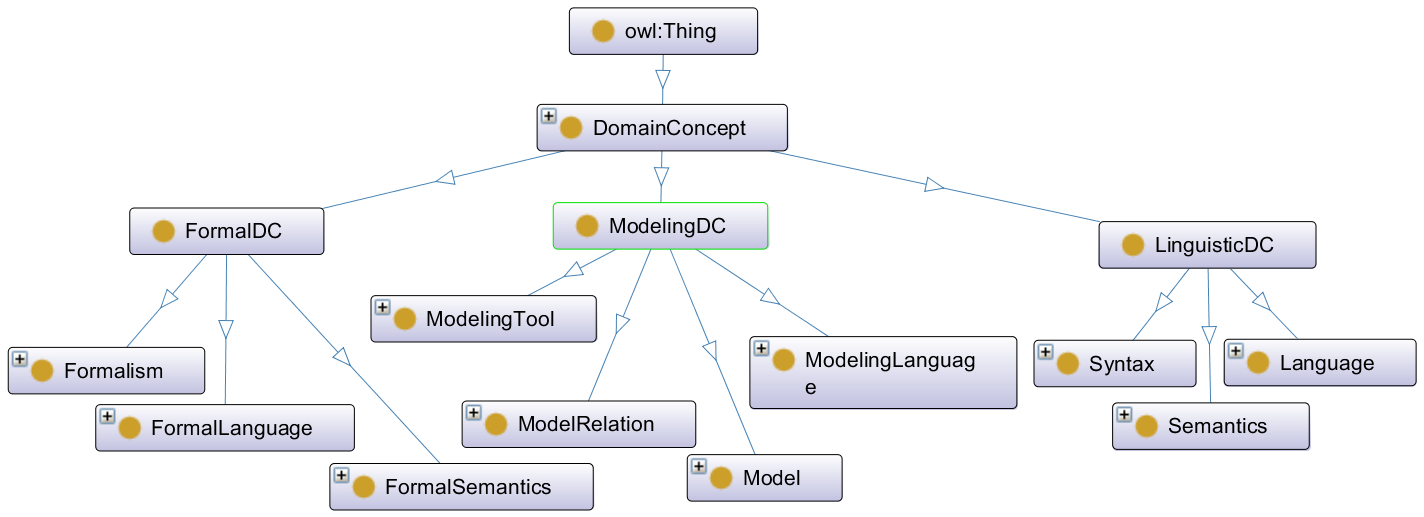
\includegraphics[width=\textwidth]{figures/mpm_ontology_overview.png}
\caption{Overview of the MPM ontology}
\label{fig:mpm_ontology_overview}
\end{figure}



\section{Domain Concepts}

This ontology of multi-paradigm modeling contains concepts divided into sub-domains as presented in the following subsections.

\subsection{ModelingDC}
\label{subsecDC:ModelingDC}

The ModelingDC subdomain organizes modeling concepts related to core modeling, multi-formalism and model management. It extends several notions introduced in a generic way by the shared ontology such as Language subclassed into ModelingLanguage and Tool subclassed into ModelingTool.

It precises the core notions of Model, ModelRelation, ModelingLanguage, AbstractSyntax, ConcreteSyntax, etc., as well as the core model management notions related to megamodeling such as Megamodel, MegamodelFragment, ModelRelation, etc.

\subsubsection{AbstractSyntax}
\label{subsubsecC:AbstractSyntax}
\didx{AbstractSyntax}

An abstract syntax is a syntax that only captures the essence of a language (its concepts and the relations between them) independently from the notation users will employ to manipulate models of the language. An abstract syntax is equivalent to the Abstract Syntax Trees (ASTs) into which code of programming languages are transformed during compilation

\textbf{Subclass of}
\begin{itemize}
	\item \textbf{Model} (see section \ref{subsubsecC:Model})
	\item \textbf{Syntax} (see section \ref{subsubsecC:Syntax})
\end{itemize}






\subsubsection{AnalysisTool}
\label{subsubsecC:AnalysisTool}
\didx{AnalysisTool}

Tools to analysis systems e.g. performance, resourceConsumption, schedulability ....

\textbf{Subclass of}
\begin{itemize}
	\item \textbf{ModelingTool} (see section \ref{subsubsecC:ModelingTool})
\end{itemize}






\subsubsection{ArchitectureDescriptionLanguage}
\label{subsubsecC:ArchitectureDescriptionLanguage}
\didx{ArchitectureDescriptionLanguage}

The notion of software architecture has been proposed, since the early 1990s by Perry and Wolf, as a software system representation composed of a set
of components with their interactions and their constraints. 
A software architecture is designed using an architectural language (may also be referred to as ADL (Architectural Description Language)), which is generally defined as any form of expression for use in architecture descriptions, according to the ISO/IEC/IEEE standard.

\textbf{Subclass of}
\begin{itemize}
	\item \textbf{ModelingLanguage} (see section \ref{subsubsecC:ModelingLanguage})
\end{itemize}






\subsubsection{AutomataBasedFormalism}
\label{subsubsecC:AutomataBasedFormalism}
\didx{AutomataBasedFormalism}

The class of formalisms that are based on automata

\textbf{Subclass of}
\begin{itemize}
	\item \textbf{Formalism} (see section \ref{subsubsecC:Formalism})
\end{itemize}






\subsubsection{BehavioralADL}
\label{subsubsecC:BehavioralADL}
\didx{BehavioralADL}

Behavioral Architectural Description Languages describe the behavior as a property of the components that constitute the architecture.

\textbf{Subclass of}
\begin{itemize}
	\item \textbf{ArchitectureDescriptionLanguage} (see section \ref{subsubsecC:ArchitectureDescriptionLanguage})
\end{itemize}






\subsubsection{BehavioralCharacteristic}
\label{subsubsecC:BehavioralCharacteristic}
\didx{BehavioralCharacteristic}

Behavioral characteristics of the formalism.

\textbf{Subclass of}
\begin{itemize}
	\item \textbf{FormalismCharacteristic} (see section \ref{subsubsecC:FormalismCharacteristic})
\end{itemize}






\subsubsection{CapturingOperation}
\label{subsubsecC:CapturingOperation}
\didx{CapturingOperation}

Capturing Operation

\textbf{Subclass of}
\begin{itemize}
	\item \textbf{TransformationRelation} (see section \ref{subsubsecC:TransformationRelation})
\end{itemize}






\subsubsection{CommunicationADL}
\label{subsubsecC:CommunicationADL}
\didx{CommunicationADL}

Communication Architecture Description Languages describe the architecture on the basis of the communication and coordination between the subcomponents, useful especially if the components are physically distributed processes.

\textbf{Subclass of}
\begin{itemize}
	\item \textbf{ArchitectureDescriptionLanguage} (see section \ref{subsubsecC:ArchitectureDescriptionLanguage})
\end{itemize}






\subsubsection{ConcreteModelingLanguage}
\label{subsubsecC:ConcreteModelingLanguage}
\didx{ConcreteModelingLanguage}

The notion of concrete language is defined as a language that comprises both an abstract syntax and a concrete syntax mapping function k.

\textbf{Subclass of}
\begin{itemize}
	\item \textbf{ModelingLanguage} (see section \ref{subsubsecC:ModelingLanguage})
\end{itemize}






\subsubsection{ConcreteSyntax}
\label{subsubsecC:ConcreteSyntax}
\didx{ConcreteSyntax}

A concrete syntax is the syntax users of the language manipulate to build models of the language. A modeling language may have several concrete syntaxes such as textual and graphical ones to improve its usability.

\textbf{Subclass of}
\begin{itemize}
	\item \textbf{Model} (see section \ref{subsubsecC:Model})
	\item \textbf{Syntax} (see section \ref{subsubsecC:Syntax})
\end{itemize}






\subsubsection{ConformanceRelation}
\label{subsubsecC:ConformanceRelation}
\didx{ConformanceRelation}

A ConformanceRelation is a subclass of the ModelRelation to relate  a Metamodel with its conforming MicroModel(s).

\textbf{Subclass of}
\begin{itemize}
	\item \textbf{ModelRelation} (see section \ref{subsubsecC:ModelRelation})
\end{itemize}






\subsubsection{ContinuousCharacteristic}
\label{subsubsecC:ContinuousCharacteristic}
\didx{ContinuousCharacteristic}

Continuous Characteristic represents the behavioral characteristics of the formalism that are continuous in nature.

\textbf{Subclass of}
\begin{itemize}
	\item \textbf{BehavioralCharacteristic} (see section \ref{subsubsecC:BehavioralCharacteristic})
\end{itemize}






\subsubsection{DiscreteCharacteristic}
\label{subsubsecC:DiscreteCharacteristic}
\didx{DiscreteCharacteristic}

Discrete Characteristic represents the behavioral characteristics of the formalism that are discrete in nature.

\textbf{Subclass of}
\begin{itemize}
	\item \textbf{BehavioralCharacteristic} (see section \ref{subsubsecC:BehavioralCharacteristic})
\end{itemize}






\subsubsection{DomainSpecificLanguage}
\label{subsubsecC:DomainSpecificLanguage}
\didx{DomainSpecificLanguage}

The DSLs are specialized languages which capture the concepts of a specific domain.

\textbf{Subclass of}
\begin{itemize}
	\item \textbf{ModelingLanguage} (see section \ref{subsubsecC:ModelingLanguage})
\end{itemize}






\subsubsection{ExecutionTool}
\label{subsubsecC:ExecutionTool}
\didx{ExecutionTool}

Execution Tool

\textbf{Subclass of}
\begin{itemize}
	\item \textbf{ModelingTool} (see section \ref{subsubsecC:ModelingTool})
\end{itemize}






\subsubsection{FlowBasedFormalism}
\label{subsubsecC:FlowBasedFormalism}
\didx{FlowBasedFormalism}

Flow-based Formalisms

\textbf{Subclass of}
\begin{itemize}
	\item \textbf{Formalism} (see section \ref{subsubsecC:Formalism})
\end{itemize}






\subsubsection{FormalLanguage}
\label{subsubsecC:FormalLanguage}
\didx{FormalLanguage}

A modeling language is said to be formal if it is based on a well-defined semantics using mathematical foundations.

\textbf{Subclass of}
\begin{itemize}
	\item \textbf{ModelingLanguage} (see section \ref{subsubsecC:ModelingLanguage})
\end{itemize}






\subsubsection{Formalism}
\label{subsubsecC:Formalism}
\didx{Formalism}

Formalisms are mathematical objects consisting of an abstract
syntax and a formal semantics. Languages are concrete
implementations of formalisms. A language has a concrete
syntax, may deviate slightly from the formalism in the
semantics that it implements, or may implement multiple
semantics (e.g., changing the type of numerical solver in a
simulation tool may change the behavior of a model). Also, a
language may implement more than one formalisms.

\textbf{Subclass of}
\begin{itemize}
	\item \textbf{FormalismDC} (see section \ref{subsubsecC:FormalismDC})
	\item \textbf{Model} (see section \ref{subsubsecC:Model})
\end{itemize}


\textbf{References}
\begin{itemize}
	
\item \bibentry{Broman2012}
\end{itemize}




\subsubsection{FormalismCharacteristic}
\label{subsubsecC:FormalismCharacteristic}
\didx{FormalismCharacteristic}

Formalism characteristic.

\textbf{Subclass of}
\begin{itemize}
	\item \textbf{FormalismDC} (see section \ref{subsubsecC:FormalismDC})
\end{itemize}






\subsubsection{FormalismDC}
\label{subsubsecC:FormalismDC}
\didx{FormalismDC}

This class groups classes related to formalisms

\textbf{Subclass of}
\begin{itemize}
	\item \textbf{ModelingDC} (see section \ref{subsecDC:ModelingDC})
\end{itemize}






\subsubsection{GraphicalSyntax}
\label{subsubsecC:GraphicalSyntax}
\didx{GraphicalSyntax}

Graphical syntax display sentences of the language as visual elements such as boxes and arrows.
However pure graphical syntax are not common and often include textual parts.

\textbf{Subclass of}
\begin{itemize}
	\item \textbf{ConcreteSyntax} (see section \ref{subsubsecC:ConcreteSyntax})
\end{itemize}






\subsubsection{HybridAutomataBasedFormalism}
\label{subsubsecC:HybridAutomataBasedFormalism}
\didx{HybridAutomataBasedFormalism}

Hybrid Automata-based Formalisms

\textbf{Subclass of}
\begin{itemize}
	\item \textbf{AutomataBasedFormalism} (see section \ref{subsubsecC:AutomataBasedFormalism})
\end{itemize}






\subsubsection{LogicBasedFormalism}
\label{subsubsecC:LogicBasedFormalism}
\didx{LogicBasedFormalism}

Logic-based Formalisms

\textbf{Subclass of}
\begin{itemize}
	\item \textbf{Formalism} (see section \ref{subsubsecC:Formalism})
\end{itemize}






\subsubsection{MegamodelFragment}
\label{subsubsecC:MegamodelFragment}
\didx{MegamodelFragment}

The fragment is not a complete megamodel, and can't be used alone. It can be reused to take part in another megamodel. (e.g. physical part, view of the system, self-adaptation .... etc.)

\textbf{Subclass of}
\begin{itemize}
	\item \textbf{Model} (see section \ref{subsubsecC:Model})
\end{itemize}





\todoAuthors{Do we add also application and configuration division here?}


\subsubsection{Metamodel}
\label{subsubsecC:Metamodel}
\didx{Metamodel}

A metamodel is a model of a model.

\textbf{Subclass of}
\begin{itemize}
	\item \textbf{Model} (see section \ref{subsubsecC:Model})
\end{itemize}






\subsubsection{MicroModelElement}
\label{subsubsecC:MicroModelElement}
\didx{MicroModelElement}

MicroModelElement represents an  atomic element contained by a MicroModel.

\textbf{Subclass of}
\begin{itemize}
	\item \textbf{Model} (see section \ref{subsubsecC:Model})
\end{itemize}






\subsubsection{Model}
\label{subsubsecC:Model}
\didx{Model}

A representation of real artifacts regardless of the metamodeling technical space. e.g. xml file, equations...etc.

\textbf{Subclass of}
\begin{itemize}
	\item \textbf{ModelingDC} (see section \ref{subsecDC:ModelingDC})
\end{itemize}






\subsubsection{ModelRelation}
\label{subsubsecC:ModelRelation}
\didx{ModelRelation}

A model relation is used to connect an arbitrary number of models.
This connects reference is defined in our ontology by the hasConnectedModels object property. 
The property has the ModelRelation for its domain and the Model class for its range.

\textbf{Subclass of}
\begin{itemize}
	\item \textbf{ModelingDC} (see section \ref{subsecDC:ModelingDC})
	\item \textbf{ModelRelation} (see section \ref{subsubsecC:ModelRelation})
\end{itemize}






\subsubsection{ModelingLanguage}
\label{subsubsecC:ModelingLanguage}
\didx{ModelingLanguage}

ModelingLanguage extends the Language subclasse from the shared ontology.

\textbf{Subclass of}
\begin{itemize}
	\item \textbf{Model} (see section \ref{subsubsecC:Model})
	\item \textbf{Language} (see section \ref{subsubsecC:Language})
\end{itemize}






\subsubsection{ModelingParadigm}
\label{subsubsecC:ModelingParadigm}
\didx{ModelingParadigm}

A modeling paradigm is a set of properties characterizing the languages (including their semantics) and workflows (development
processes) employed to develop systems.

\textbf{Subclass of}
\begin{itemize}
	\item \textbf{ModelingDC} (see section \ref{subsecDC:ModelingDC})
\end{itemize}






\subsubsection{ModelingTool}
\label{subsubsecC:ModelingTool}
\didx{ModelingTool}

Tools to model the system.

\textbf{Subclass of}
\begin{itemize}
	\item \textbf{Model} (see section \ref{subsubsecC:Model})
	\item \textbf{Tool} (see section \ref{subsubsecC:Tool})
\end{itemize}






\subsubsection{PetriNetBasedFormalism}
\label{subsubsecC:PetriNetBasedFormalism}
\didx{PetriNetBasedFormalism}

Petri nets (also known as a place/transition net or P/T net) are formalisms for the description of distributed systems.

\textbf{Subclass of}
\begin{itemize}
	\item \textbf{Formalism} (see section \ref{subsubsecC:Formalism})
\end{itemize}






\subsubsection{ProgrammingLanguage}
\label{subsubsecC:ProgrammingLanguage}
\didx{ProgrammingLanguage}

The programming languages can be seen as a subset of modeling languages.

\textbf{Subclass of}
\begin{itemize}
	\item \textbf{ModelingLanguage} (see section \ref{subsubsecC:ModelingLanguage})
\end{itemize}






\subsubsection{RefinementRelation}
\label{subsubsecC:RefinementRelation}
\didx{RefinementRelation}

Example of a  transformation relation.

\textbf{Subclass of}
\begin{itemize}
	\item \textbf{TransformationRelation} (see section \ref{subsubsecC:TransformationRelation})
\end{itemize}






\subsubsection{RuntimeTool}
\label{subsubsecC:RuntimeTool}
\didx{RuntimeTool}

Runtime Tool

\textbf{Subclass of}
\begin{itemize}
	\item \textbf{ModelingTool} (see section \ref{subsubsecC:ModelingTool})
\end{itemize}






\subsubsection{SemanticDomain}
\label{subsubsecC:SemanticDomain}
\didx{SemanticDomain}

According to Wikipedia, a semantic domain is defined as a specific place that shares a set of meanings, or a language that holds it.

\textbf{Subclass of}
\begin{itemize}
	\item \textbf{Model} (see section \ref{subsubsecC:Model})
\end{itemize}






\subsubsection{SemanticMappingRelation}
\label{subsubsecC:SemanticMappingRelation}
\didx{SemanticMappingRelation}

A semantic mapping relation.

\textbf{Subclass of}
\begin{itemize}
	\item \textbf{ModelRelation} (see section \ref{subsubsecC:ModelRelation})
\end{itemize}






\subsubsection{SimulationTool}
\label{subsubsecC:SimulationTool}
\didx{SimulationTool}

Simulation Tool

\textbf{Subclass of}
\begin{itemize}
	\item \textbf{ModelingTool} (see section \ref{subsubsecC:ModelingTool})
\end{itemize}






\subsubsection{StructuralADL}
\label{subsubsecC:StructuralADL}
\didx{StructuralADL}

Structure Architectural Definition Languages have the capability of defining the topological/heirarchical structure of the components of the architecture. For example, pipe-and-filter architectures.

\textbf{Subclass of}
\begin{itemize}
	\item \textbf{ArchitectureDescriptionLanguage} (see section \ref{subsubsecC:ArchitectureDescriptionLanguage})
\end{itemize}






\subsubsection{StructuralConstraintLanguage}
\label{subsubsecC:StructuralConstraintLanguage}
\didx{StructuralConstraintLanguage}

A modeling language for expressing constraints.

\textbf{Subclass of}
\begin{itemize}
	\item \textbf{ModelingLanguage} (see section \ref{subsubsecC:ModelingLanguage})
\end{itemize}






\subsubsection{StructureCharacteristic}
\label{subsubsecC:StructureCharacteristic}
\didx{StructureCharacteristic}

Structural characteristics of the formalism

\textbf{Subclass of}
\begin{itemize}
	\item \textbf{FormalismCharacteristic} (see section \ref{subsubsecC:FormalismCharacteristic})
\end{itemize}






\subsubsection{SynchronizationRelation}
\label{subsubsecC:SynchronizationRelation}
\didx{SynchronizationRelation}

Example of a  transformation relation.

\textbf{Subclass of}
\begin{itemize}
	\item \textbf{TransformationRelation} (see section \ref{subsubsecC:TransformationRelation})
\end{itemize}






\subsubsection{SyntaxMappingRelation}
\label{subsubsecC:SyntaxMappingRelation}
\didx{SyntaxMappingRelation}

Abstract and concrete syntaxes are related via a SyntaxMappingRelation  class that associates element(s) of a concrete syntax to represent element(s) of the abstract syntax.

\textbf{Subclass of}
\begin{itemize}
	\item \textbf{ModelRelation} (see section \ref{subsubsecC:ModelRelation})
\end{itemize}






\subsubsection{TextualSyntax}
\label{subsubsecC:TextualSyntax}
\didx{TextualSyntax}

A textual syntax consists of sequences of characters taken from an alphabet and grouped into words or tokens. 
Only some sequences of words or sentences are considered valid and the set of all valid sentences is said to make up the language.

\textbf{Subclass of}
\begin{itemize}
	\item \textbf{ConcreteSyntax} (see section \ref{subsubsecC:ConcreteSyntax})
\end{itemize}






\subsubsection{TimedAutomataBasedFormalism}
\label{subsubsecC:TimedAutomataBasedFormalism}
\didx{TimedAutomataBasedFormalism}

Timed Automata-based Formalisms

\textbf{Subclass of}
\begin{itemize}
	\item \textbf{HybridAutomataBasedFormalism} (see section \ref{subsubsecC:HybridAutomataBasedFormalism})
\end{itemize}






\subsubsection{TimedCharacteristic}
\label{subsubsecC:TimedCharacteristic}
\didx{TimedCharacteristic}

Timed Characteristic  represents the behavioral characteristics of the formalism that are time-bound.

\textbf{Subclass of}
\begin{itemize}
	\item \textbf{BehavioralCharacteristic} (see section \ref{subsubsecC:BehavioralCharacteristic})
\end{itemize}






\subsubsection{TraceabilityRelation}
\label{subsubsecC:TraceabilityRelation}
\didx{TraceabilityRelation}

A traceability relation is a technique to provide a relationship between requirements, design, and final implementation of a system.

\textbf{Subclass of}
\begin{itemize}
	\item \textbf{ModelRelation} (see section \ref{subsubsecC:ModelRelation})
\end{itemize}






\subsubsection{TransformationLanguage}
\label{subsubsecC:TransformationLanguage}
\didx{TransformationLanguage}

A langauge to specify model transformations.

\textbf{Subclass of}
\begin{itemize}
	\item \textbf{ModelingLanguage} (see section \ref{subsubsecC:ModelingLanguage})
\end{itemize}






\subsubsection{TransformationRelation}
\label{subsubsecC:TransformationRelation}
\didx{TransformationRelation}

A Transformation Relation

\textbf{Subclass of}
\begin{itemize}
	\item \textbf{ModelRelation} (see section \ref{subsubsecC:ModelRelation})
\end{itemize}






\subsubsection{TransformationTool}
\label{subsubsecC:TransformationTool}
\didx{TransformationTool}

Transformation Tool

\textbf{Subclass of}
\begin{itemize}
	\item \textbf{ModelingTool} (see section \ref{subsubsecC:ModelingTool})
\end{itemize}






\subsubsection{UncertaintyCharacteristic}
\label{subsubsecC:UncertaintyCharacteristic}
\didx{UncertaintyCharacteristic}

Uncertainty Characteristic  represents the behavioral characteristics of the formalism that have uncertainty.

\textbf{Subclass of}
\begin{itemize}
	\item \textbf{BehavioralCharacteristic} (see section \ref{subsubsecC:BehavioralCharacteristic})
\end{itemize}






\subsubsection{VisualizationTool}
\label{subsubsecC:VisualizationTool}
\didx{VisualizationTool}

Visualization Tool

\textbf{Subclass of}
\begin{itemize}
	\item \textbf{ModelingTool} (see section \ref{subsubsecC:ModelingTool})
\end{itemize}

\section{Properties}
\label{sec:mpm:properties}


\subsection{hasAbstractSyntax}
\label{subsecP:hasAbstractSyntax}
The hasAbstractSyntax object property is a subproperty of the hasSyntax object property of the linguistic subdomain to relate the  ModelingLanguage and AbstractSyntax classes.

Subproperty of:
\begin{itemize}
	\item \textbf{hasSyntax} (see section \ref{subsecP:hasSyntax})
\end{itemize}


Domains:
\begin{itemize}
	\item \textbf{ModelingLanguage} (see section \ref{subsubsecC:ModelingLanguage})
\end{itemize}


Ranges:
\begin{itemize}
	\item \textbf{AbstractSyntax} (see section \ref{subsubsecC:AbstractSyntax})
\end{itemize}




\subsection{hasAbstractSyntaxSem}
\label{subsecP:hasAbstractSyntaxSem}
The hasAbstractSyntaxSem object property links the mapping relation to the mapped abstract syntax.

Subproperty of:
\begin{itemize}
	\item \textbf{hasConnectedModel} (see section \ref{subsecP:hasConnectedModel})
\end{itemize}


Domains:
\begin{itemize}
	\item \textbf{SemanticMappingRelation} (see section \ref{subsubsecC:SemanticMappingRelation})
\end{itemize}


Ranges:
\begin{itemize}
	\item \textbf{AbstractSyntax} (see section \ref{subsubsecC:AbstractSyntax})
\end{itemize}




\subsection{hasCharacteristic}
\label{subsecP:hasCharacteristic}
The hasCharacteristics relates a Formalism with a characteristic.

Subproperty of:
None


Domains:
\begin{itemize}
	\item \textbf{Formalism} (see section \ref{subsubsecC:Formalism})
\end{itemize}


Ranges:
\begin{itemize}
	\item \textbf{FormalismCharacteristic} (see section \ref{subsubsecC:FormalismCharacteristic})
\end{itemize}




\subsection{hasConcreteSyntax}
\label{subsecP:hasConcreteSyntax}
The hasAbstractSyntax object property is a subproperty of the hasSyntax object property of the linguistic subdomain, relating a ModelingLanguage with its  AbstractSyntax.

Subproperty of:
None


Domains:
\begin{itemize}
	\item \textbf{SyntaxMappingRelation} (see section \ref{subsubsecC:SyntaxMappingRelation})
\end{itemize}


Ranges:
\begin{itemize}
	\item \textbf{ConcreteSyntax} (see section \ref{subsubsecC:ConcreteSyntax})
\end{itemize}




\subsection{hasConformedModel}
\label{subsecP:hasConformedModel}
The hasConnectedModels object property links a  ConformanceRelation to MicroModel.

Subproperty of:
\begin{itemize}
	\item \textbf{hasConnectedModel} (see section \ref{subsecP:hasConnectedModel})
\end{itemize}


Domains:
\begin{itemize}
	\item \textbf{ConformanceRelation} (see section \ref{subsubsecC:ConformanceRelation})
\end{itemize}


Ranges:
\begin{itemize}
	\item \textbf{Micromodel} (see section \ref{subsubsecC:Micromodel})
\end{itemize}




\subsection{hasConnectedModel}
\label{subsecP:hasConnectedModel}
The model relation is used to connect an arbitrary number of models. This connects reference is defined in our ontology by the hasConnectedModels object property.

Subproperty of:
None


Domains:
\begin{itemize}
	\item \textbf{ModelRelation} (see section \ref{subsubsecC:ModelRelation})
\end{itemize}


Ranges:
\begin{itemize}
	\item \textbf{Model} (see section \ref{subsubsecC:Model})
\end{itemize}




\subsection{hasContainedMegamodelFragments}
\label{subsecP:hasContainedMegamodelFragments}
It describes the relation between megamodel and its fragments.

Subproperty of:
\begin{itemize}
	\item \textbf{hasContainedModels} (see section \ref{subsecP:hasContainedModels})
\end{itemize}


Domains:
\begin{itemize}
	\item \textbf{Megamodel} (see section \ref{subsubsecC:Megamodel})
\end{itemize}


Ranges:
\begin{itemize}
	\item \textbf{MegamodelFragment} (see section \ref{subsubsecC:MegamodelFragment})
\end{itemize}




\subsection{hasContainedModelElements}
\label{subsecP:hasContainedModelElements}
It describes the relation between micromodel and its elements.

Subproperty of:
\begin{itemize}
	\item \textbf{hasContainedModels} (see section \ref{subsecP:hasContainedModels})
\end{itemize}


Domains:
\begin{itemize}
	\item \textbf{Micromodel} (see section \ref{subsubsecC:Micromodel})
\end{itemize}


Ranges:
\begin{itemize}
	\item \textbf{MicroModelElement} (see section \ref{subsubsecC:MicroModelElement})
\end{itemize}




\subsection{hasContainedModelRelations}
\label{subsecP:hasContainedModelRelations}
A model relation also needs to be contained in a model and therefore we create the hasContainedModelRelations object property whose domain is Model and range ModelRelation.

Subproperty of:
None


Domains:
\begin{itemize}
	\item \textbf{Model} (see section \ref{subsubsecC:Model})
\end{itemize}


Ranges:
\begin{itemize}
	\item \textbf{ModelRelation} (see section \ref{subsubsecC:ModelRelation})
\end{itemize}




\subsection{hasContainedModels}
\label{subsecP:hasContainedModels}
It describes a recursive relation. e.g. MegaModelFragment hasModel xModel ...

Subproperty of:
None


Domains:
\begin{itemize}
	\item \textbf{Model} (see section \ref{subsubsecC:Model})
\end{itemize}


Ranges:
\begin{itemize}
	\item \textbf{Model} (see section \ref{subsubsecC:Model})
\end{itemize}




\subsection{hasContextRelation}
\label{subsecP:hasContextRelation}
A model relation may exist in the context of another model relation. This is expressed by  the hasContextRelation object property in the ontology. An example of such contextual relation may be a relation between to model elements that can only exist after a relation has first been created between their respective containing parent elements.

Subproperty of:
None


Domains:
\begin{itemize}
	\item \textbf{ModelRelation} (see section \ref{subsubsecC:ModelRelation})
\end{itemize}


Ranges:
\begin{itemize}
	\item \textbf{ModelRelation} (see section \ref{subsubsecC:ModelRelation})
\end{itemize}




\subsection{hasCoreLanguage}
\label{subsecP:hasCoreLanguage}
\todoAuthors{Provide ``rdfs:comment'' annotation in ontology}

Subproperty of:
None


Domains:
\begin{itemize}
	\item \textbf{ModelingLanguage} (see section \ref{subsubsecC:ModelingLanguage})
\end{itemize}


Ranges:
\begin{itemize}
	\item \textbf{ModelingLanguage} (see section \ref{subsubsecC:ModelingLanguage})
\end{itemize}




\subsection{hasInputModel}
\label{subsecP:hasInputModel}
It describes the input model for a model relation.

Subproperty of:
None


Domains:
\begin{itemize}
	\item \textbf{ModelRelation} (see section \ref{subsubsecC:ModelRelation})
\end{itemize}


Ranges:
\begin{itemize}
	\item \textbf{Model} (see section \ref{subsubsecC:Model})
\end{itemize}




\subsection{hasLanguage}
\label{subsecP:hasLanguage}
\todoAuthors{Provide ``rdfs:comment'' annotation in ontology}

Subproperty of:
None


Domains:
\begin{itemize}
	\item \textbf{Micromodel} (see section \ref{subsubsecC:Micromodel})
\end{itemize}


Ranges:
\begin{itemize}
	\item \textbf{ModelingLanguage} (see section \ref{subsubsecC:ModelingLanguage})
\end{itemize}




\subsection{hasLanguageFragment}
\label{subsecP:hasLanguageFragment}
\todoAuthors{Provide ``rdfs:comment'' annotation in ontology}

Subproperty of:
None


Domains:
\begin{itemize}
	\item \textbf{ModelingLanguage} (see section \ref{subsubsecC:ModelingLanguage})
\end{itemize}


Ranges:
\begin{itemize}
	\item \textbf{LanguageFragment} (see section \ref{subsubsecC:LanguageFragment})
\end{itemize}




\subsection{hasMetamodel}
\label{subsecP:hasMetamodel}
The hasMetamodel object property is a subproperty of the hasConnectedModels object property with its domain and range respectively refined to ConformanceRelation and Metamodel

Subproperty of:
\begin{itemize}
	\item \textbf{hasConnectedModel} (see section \ref{subsecP:hasConnectedModel})
\end{itemize}


Domains:
\begin{itemize}
	\item \textbf{ConformanceRelation} (see section \ref{subsubsecC:ConformanceRelation})
\end{itemize}


Ranges:
\begin{itemize}
	\item \textbf{Metamodel} (see section \ref{subsubsecC:Metamodel})
\end{itemize}




\subsection{hasOutputModel}
\label{subsecP:hasOutputModel}
It describes the output model for a model relation.

Subproperty of:
None


Domains:
\begin{itemize}
	\item \textbf{ModelRelation} (see section \ref{subsubsecC:ModelRelation})
\end{itemize}


Ranges:
\begin{itemize}
	\item \textbf{Model} (see section \ref{subsubsecC:Model})
\end{itemize}




\subsection{hasSemanticDomain}
\label{subsecP:hasSemanticDomain}
The hasSemanticDomain object properties links the mapping relation to  its semantic domain.

Subproperty of:
\begin{itemize}
	\item \textbf{hasConnectedModel} (see section \ref{subsecP:hasConnectedModel})
\end{itemize}


Domains:
\begin{itemize}
	\item \textbf{SemanticMappingRelation} (see section \ref{subsubsecC:SemanticMappingRelation})
\end{itemize}


Ranges:
\begin{itemize}
	\item \textbf{SemanticDomain} (see section \ref{subsubsecC:SemanticDomain})
\end{itemize}




\subsection{hasSpecification}
\label{subsecP:hasSpecification}
a TransformationRelation class is a subclass of the ModelRelation class with an object property hasSpecification
to relate the transformation relation to its specification.

Subproperty of:
None


Domains:
\begin{itemize}
	\item \textbf{TransformationRelation} (see section \ref{subsubsecC:TransformationRelation})
\end{itemize}


Ranges:
\begin{itemize}
	\item \textbf{Micromodel} (see section \ref{subsubsecC:Micromodel})
\end{itemize}




\subsection{hasSyntaxMapping}
\label{subsecP:hasSyntaxMapping}
The hasSyntaxMapping relates  a ConcreteModelingLanguage to its SyntaxMappingRelation.

Subproperty of:
None


Domains:
\begin{itemize}
	\item \textbf{ConcreteModelingLanguage} (see section \ref{subsubsecC:ConcreteModelingLanguage})
\end{itemize}


Ranges:
\begin{itemize}
	\item \textbf{SyntaxMappingRelation} (see section \ref{subsubsecC:SyntaxMappingRelation})
\end{itemize}




\subsection{hasTool}
\label{subsecP:hasTool}
This object property relates a modelling language to the tool(s) that implement it,

Subproperty of:
None


Domains:
\begin{itemize}
	\item \textbf{ModelingLanguage} (see section \ref{subsubsecC:ModelingLanguage})
\end{itemize}


Ranges:
\begin{itemize}
	\item \textbf{ModelingTool} (see section \ref{subsubsecC:ModelingTool})
\end{itemize}




\subsection{hasTraceabilityRelation}
\label{subsecP:hasTraceabilityRelation}
The hasContainedModelRelations is refined into the hasTraceabilityRelation with the domain and the range respectively refined into TraceabilityModel and TraceabilityRelation.

Subproperty of:
\begin{itemize}
	\item \textbf{hasContainedModelRelations} (see section \ref{subsecP:hasContainedModelRelations})
\end{itemize}


Domains:
\begin{itemize}
	\item \textbf{TraceabilityModel} (see section \ref{subsubsecC:TraceabilityModel})
\end{itemize}


Ranges:
\begin{itemize}
	\item \textbf{TraceabilityRelation} (see section \ref{subsubsecC:TraceabilityRelation})
\end{itemize}




\subsection{hasTranformationSpecification}
\label{subsecP:hasTranformationSpecification}
The hasTranformationSpecifications object property relates an activity performer resource to the transformation relations it executes.

Subproperty of:
None


Domains:
\begin{itemize}
	\item \textbf{ActivityPerformer} (see section \ref{subsubsecC:ActivityPerformer})
\end{itemize}


Ranges:
\begin{itemize}
	\item \textbf{TransformationRelation} (see section \ref{subsubsecC:TransformationRelation})
\end{itemize}




\subsection{hasUsedModels}
\label{subsecP:hasUsedModels}
This propoerty relates the MegaModel Fragment to the MicroModel(s) it incorporates.

Subproperty of:
None


Domains:
\begin{itemize}
	\item \textbf{MegamodelFragment} (see section \ref{subsubsecC:MegamodelFragment})
\end{itemize}


Ranges:
\begin{itemize}
	\item \textbf{Micromodel} (see section \ref{subsubsecC:Micromodel})
\end{itemize}




\subsection{isBasedOn}
\label{subsecP:isBasedOn}
The relation defines the formalism for a formal language. It is an inverse of hasLanguage.

Subproperty of:
None


Domains:
\begin{itemize}
	\item \textbf{ModelingLanguage} (see section \ref{subsubsecC:ModelingLanguage})
\end{itemize}


Ranges:
\begin{itemize}
	\item \textbf{Formalism} (see section \ref{subsubsecC:Formalism})
\end{itemize}




\subsection{isEnvironmentFor}
\label{subsecP:isEnvironmentFor}
This relation is used to relate a modelling tool to its extension(s). The original modelling tool serves as an environment for the development and operation of the tool extension.

Subproperty of:
None


Domains:
\begin{itemize}
	\item \textbf{ModelingTool} (see section \ref{subsubsecC:ModelingTool})
\end{itemize}


Ranges:
\begin{itemize}
	\item \textbf{ToolExtension} (see section \ref{subsubsecC:ToolExtension})
\end{itemize}




\subsection{isImplementedBy}
\label{subsecP:isImplementedBy}
This property relates a modeling language to the formalism(s) it implements.

Subproperty of:
None


Domains:
\begin{itemize}
	\item \textbf{Formalism} (see section \ref{subsubsecC:Formalism})
\end{itemize}


Ranges:
\begin{itemize}
	\item \textbf{ModelingLanguage} (see section \ref{subsubsecC:ModelingLanguage})
\end{itemize}




\subsection{isToolExtensionFor}
\label{subsecP:isToolExtensionFor}
This property is the inverse of the isEnvironmentFor object property which relates a modelling tool and its extension(s).

Subproperty of:
None


Domains:
\begin{itemize}
	\item \textbf{ToolExtension} (see section \ref{subsubsecC:ToolExtension})
\end{itemize}


Ranges:
\begin{itemize}
	\item \textbf{ModelingTool} (see section \ref{subsubsecC:ModelingTool})
\end{itemize}




\subsection{isToolFor}
\label{subsecP:isToolFor}
This property is the inverse of hasTool object property.

Subproperty of:
None


Domains:
\begin{itemize}
	\item \textbf{ModelingTool} (see section \ref{subsubsecC:ModelingTool})
\end{itemize}


Ranges:
\begin{itemize}
	\item \textbf{ModelingLanguage} (see section \ref{subsubsecC:ModelingLanguage})
\end{itemize}





\label{sec:Ontology-MML}

% ========================================================
\chapter{Ontology of Multi-Paradigm Modeling for Cyber-Physical Systems}
\label{ch:mpm4cps}
\STATUS{For the deliverables, this needs to be completed with the basic examples of Bronan et al. dusplayed in the ontology and references to the paper. For the book, we should also capture the viewpoints for the Ensemble-Based and HPI CPS lab examples with the ontology, which may trigger some changes in the ontology as new concepts may be required.}

\section{Introduction}
%\todo{\textbf{TODO Dominique}}

This ontology of MPM for CPS provides cross-cutting concepts between the two domains of CPS and MPM. At the current stage of development, this ontology only contains a limited number of classes related to \emph{viewpoints} inspired from \cite{Broman2012}. 

%****************************************************************************************************************************************
% File: mpm4cps-ontology.tex
%
% This file is automatically generated. Please do not edit!
%****************************************************************************************************************************************
\section{Ontology Overview}

The OWL MPM4CPS ontology that defines cross-cutting concepts between the Shared, MPM and CPS ontologies.

Figure \ref{fig:mpm_ontology_overview} shows an overview of the MPM4CPS ontology. The details of each concept are
provided in the following subsections.

\begin{figure}[!htb]
\centering
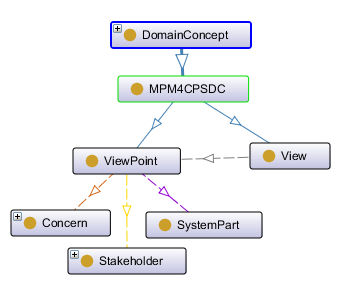
\includegraphics[width=0.5\textwidth]{figures/mpm4cps_overview.png}
\caption{Overview of the MPM4CPS ontology}
\label{fig:mpm4cps_ontology_overview}
\end{figure}



\section{Domain Concepts}

This ontology of multi-paradigm modeling contains concepts divided into sub-domains as presented in the following subsections.

\subsection{MPM4CPSDC}
\label{subsecDC:MPM4CPSDC}

MPM4CPSDC domain concept class

\subsubsection{ModelBasedEngineeringEnv}
\label{subsubsecC:ModelBasedEngineeringEnv}
\didx{ModelBasedEngineeringEnv}

In order to define our modeling paradigm notion, we first subclass the EngineeringEnvironment class of the Shared ontology by the ModelBasedEngineeringEnv class.

\textbf{Subclass of}
\begin{itemize}
	\item \textbf{MPM4CPSDC} (see section \ref{subsecDC:MPM4CPSDC})
	\item \textbf{EngineeringEnvironment} (see section \ref{subsubsecC:EngineeringEnvironment})
\end{itemize}






\subsubsection{ModelBasedProcess}
\label{subsubsecC:ModelBasedProcess}
\didx{ModelBasedProcess}

The Process class of the Shared ontology is refined into the ModelBasedProcess class to represent all processes that manipulate models instead of data fields.

\textbf{Subclass of}
\begin{itemize}
	\item \textbf{MPM4CPSDC} (see section \ref{subsecDC:MPM4CPSDC})
	\item \textbf{ModelBasedEngineeringArtifact} (see section \ref{subsubsecC:ModelBasedEngineeringArtifact})
	\item \textbf{Process} (see section \ref{subsubsecC:Process})
\end{itemize}






\subsubsection{View}
\label{subsubsecC:View}
\didx{View}

A viewpoint governs an architecture view.

\textbf{Subclass of}
\begin{itemize}
	\item \textbf{MPM4CPSDC} (see section \ref{subsecDC:MPM4CPSDC})
	\item \textbf{View} (see section \ref{subsubsecC:View})
\end{itemize}





\todoAuthors{Finally, we create another object property to relate a view to its employed models.}


\subsubsection{ViewPoint}
\label{subsubsecC:ViewPoint}
\didx{ViewPoint}

According to the IEEE 42010 standard, a viewpoint frames the concerns of stakeholders.

\textbf{Subclass of}
\begin{itemize}
	\item \textbf{MPM4CPSDC} (see section \ref{subsecDC:MPM4CPSDC})
	\item \textbf{ViewPoint} (see section \ref{subsubsecC:ViewPoint})
\end{itemize}

\section{Properties}


\subsection{hasFramedConcerns}
\label{subsecP:hasFramedConcerns}
The hasFramedConcerns object property relates a viewpoint to a set of framed concerns as defined in the Shared ontology.

Subproperty of:
None


Domains:
\begin{itemize}
	\item \textbf{ViewPoint} (see section \ref{subsubsecC:ViewPoint})
\end{itemize}


Ranges:
\begin{itemize}
	\item \textbf{Concern} (see section \ref{subsubsecC:Concern})
\end{itemize}




\subsection{hasGovernedView}
\label{subsecP:hasGovernedView}
The hasGovernedView object property relates a viewpoint to its view.

Subproperty of:
None


Domains:
\begin{itemize}
	\item \textbf{ViewPoint} (see section \ref{subsubsecC:ViewPoint})
\end{itemize}


Ranges:
\begin{itemize}
	\item \textbf{View} (see section \ref{subsubsecC:View})
\end{itemize}




\subsection{hasGoverningView}
\label{subsecP:hasGoverningView}
A viewpoint governs an architecture view.

Subproperty of:
None


Domains:
\begin{itemize}
	\item \textbf{View} (see section \ref{subsubsecC:View})
\end{itemize}


Ranges:
\begin{itemize}
	\item \textbf{ViewPoint} (see section \ref{subsubsecC:ViewPoint})
\end{itemize}




\subsection{hasStakeholders}
\label{subsecP:hasStakeholders}
The hasStakeholders  object property relates a ViewPoint to its Stakeholder.

Subproperty of:
None


Domains:
\begin{itemize}
	\item \textbf{ViewPoint} (see section \ref{subsubsecC:ViewPoint})
\end{itemize}


Ranges:
\begin{itemize}
	\item \textbf{Stakeholder} (see section \ref{subsubsecC:Stakeholder})
\end{itemize}




\subsection{hasSupportingMegamodelFragments}
\label{subsecP:hasSupportingMegamodelFragments}
The hasSupportingMegamodelFragments object property  relates a viewpoint to a set of supporting megamodel fragments.

Subproperty of:
None


Domains:
\begin{itemize}
	\item \textbf{ViewPoint} (see section \ref{subsubsecC:ViewPoint})
\end{itemize}


Ranges:
None




\subsection{hasSystemConstituentElements}
\label{subsecP:hasSystemConstituentElements}
The hasSystemConstituentElements object property relates a viewpoint with its system constituents or parts.

Subproperty of:
None


Domains:
\begin{itemize}
	\item \textbf{ViewPoint} (see section \ref{subsubsecC:ViewPoint})
\end{itemize}


Ranges:
None




\subsection{hasViewpoint}
\label{subsecP:hasViewpoint}
A set of viewpoints can be linked to a process through an object property hasViewpoint, so that data types are declared as the elements grouped under the associated megamodel fragment.

Subproperty of:
None


Domains:
\begin{itemize}
	\item \textbf{ModelBasedProcess} (see section \ref{subsubsecC:ModelBasedProcess})
\end{itemize}


Ranges:
\begin{itemize}
	\item \textbf{ViewPoint} (see section \ref{subsubsecC:ViewPoint})
\end{itemize}




\subsection{isSupportedBy}
\label{subsecP:isSupportedBy}
A ViewPoint is supported by a Formalism.

Subproperty of:
None


Domains:
\begin{itemize}
	\item \textbf{ViewPoint} (see section \ref{subsubsecC:ViewPoint})
\end{itemize}


Ranges:
\begin{itemize}
	\item \textbf{Formalism} (see section \ref{subsubsecC:Formalism})
\end{itemize}






% \section{Ontology Overview}
% 
% Figure \ref{fig:mpm4cps_overview} shows the classes and properties of the MPM4CPS ontology. The MPM4CPSDC class groups the Viewpoint and View classes to constitute the MPM4CPS domain.
% 
% \begin{figure}[!htb]
% \centering
% 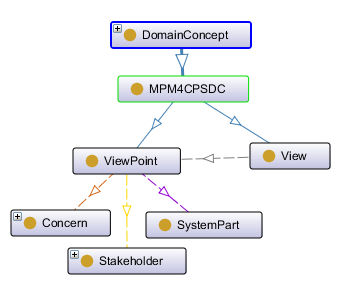
\includegraphics[width=0.5\textwidth]{figures/mpm4cps_overview.png}
% \caption{Overview of the MPM4CPS ontology}
% \label{fig:mpm4cps_overview}
% \end{figure}
% 
% A viewpoint relates the \emph{concerns} of \emph{stakeholders} with \emph{parts} of the system of interest. For example, a \emph{control design performance} viewpoint may relate the controller designer with the concern of performance and the controller, software, sensors and actuators, computing platform and physical plant parts of the system.
% 
% In the next version of this ontology, other classes that relate the MPM and CPS domains will be added as needed.
% 
% \section{Domain Concepts}
% 
% \section{Properties}


% ========================================================
\chapter{Examples}
\label{ch:examples}
\label{ch:catalog}

\section{Ensemble-based CPS}  

\subsection{Overview}
%\STATUS{ready for review}
An Ensemble-Based Cyber-Physical System (EBCPS) is an emergent system\uidx{System} that is distributed\uidx{Distributed}, decentralized, dynamic, self-adaptive and scalable. It consists of autonomous components\uidx{Component} and forms ensembles of them depending on the context in the aim of achieving determined goals (i.e. organizing\uidx{Organization} and decision-making). More specifically, the composition\uidx{Compositionality} of components changes according to the fact of having the components appear and disappear dynamically, in addition to the unexpected changes in the environment and new requirements. There are many applications in different domains such as Traffic and Transport, Robotics, and Clouds. For instance, an ensemble of vehicle planning for optimal route with considering the road and traffic conditions. 

The interest of building such systems\uidx{System} was reflected in many European projects such as ASCENS\footnote{\url{http://www.ascens-ist.eu/}}, ALLOW Ensembles\footnote{\url{http://www.allow-ensembles.eu/}} and FoCAS \footnote{\url{http://www.focas.eu/}}, which are FP7 projects. ASCENS is oriented towards design and verification, while ALLOW Ensembles is more oriented towards performance. More specifically, ASCENS targets formalizing and modeling ensembles of autonomic-service components (SCs) that depend on knowledge units (K). It considers also the expression of self-adaption and provides tools and use cases. ALLOW Ensembles focuses on developing algorithms that improve ensembles utility and system dependability. Both previous projects are involved in FoCAS, which is a platform for communities that care about developing Collective Adaptive Systems (CAS\' s).

As part from ASCENS project, a formalism language was introduced to express the ensembles called Service Component Ensemble Language (SCEL) Figure~\ref{fig:Service_Component}. The language allows to define Knowledge, Behaviors\uidx{Behavioural}, Aggregations, and Policies. It allows the developer to define  interfaces with attributes or knowledge for Service Components (SCs) and their behavior using processes\uidx{Process}. Also, the developer can define the Service Component Ensembles (SCEs) and the conditions or policies to form them. The ensembles are responsible for exchanging knowledge between the components. Each ensemble evaluates the constraints\uidx{Constraint} over the interface attributes of the involved components. The support of context-awareness comes from using attributes in the constraint evaluation\uidx{Constraint} of forming ensembles.  
\begin{figure}[!htb]
\centering
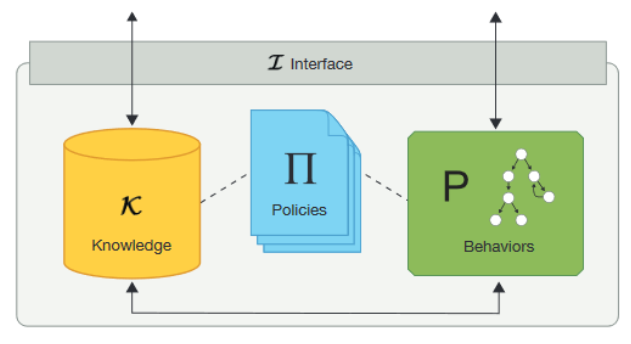
\includegraphics[scale=0.44]{figures/ServiceComponent.PNG}
\caption{Service Component}
\label{fig:Service_Component}
\end{figure}

Furthermore, ASCENS provides many tools for modeling (e.g. HELENA, KnowLang, DEECo) and for simulation (e.g. ARGoS, SPL, jDEECo Java, SimSOTA). Additionally, the concepts are presented in three use cases in different domains, which are: Clouds, Traffic and Transport, and Robotics.


\subsection{Dependable Emergent Ensembles of Components (DEECo)}
\uidx{Dependability}
To manifest the new concepts of EBCPS, the Department of Distributed and Dependable Systems (d3s: \url{http://d3s.mff.cuni.cz/}) at Charles University in Prague developed an EBCPS toolchain that is used as development environment which merges the concepts of emergent systems with the CPS parts\uidx{SystemPart} (i.e. physical, computational and network). More specifically, the parts that will be explained here are requirements, design, runtime, self-adaptation, analysis, composition and simulation. Moreover, there are many integrations and transformations\uidx{TransformationOperation} between the models.

\begin{figure}[!h]
\centering
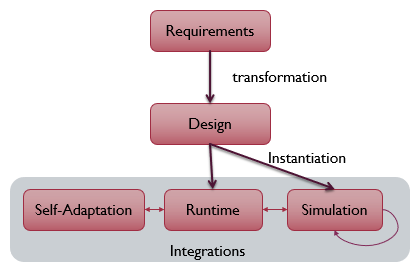
\includegraphics[width=\textwidth]{figures/deeco_map.PNG}
\caption{Overview of the models provided by DEECo and their relations}
\label{fig:deeco_map}
\end{figure}

\subsubsection{Requirements}
Starting with modeling EBCPS requirements, Invariant Refinement Method (IRM) \cite{Keznikl:2013:DEC:2465449.2465457} (see  Figure~\ref{fig:irm}, which is developed in Epsilon, is used to represent the tree of invariants and assumptions for the system. The tree ends with leaves of two types: 1) processes\uidx{Process} which are part of a component\uidx{Component}, 2) or exchange knowledge between components\uidx{Component} which are ensembles. Simply put, the IRM allows to connect the requirements to the architecture entities directly. Later on, the developer can transform the IRM model to code which is Java for the current represented tool-chain under DEECo specification.

\begin{figure}[!htb]
\centering
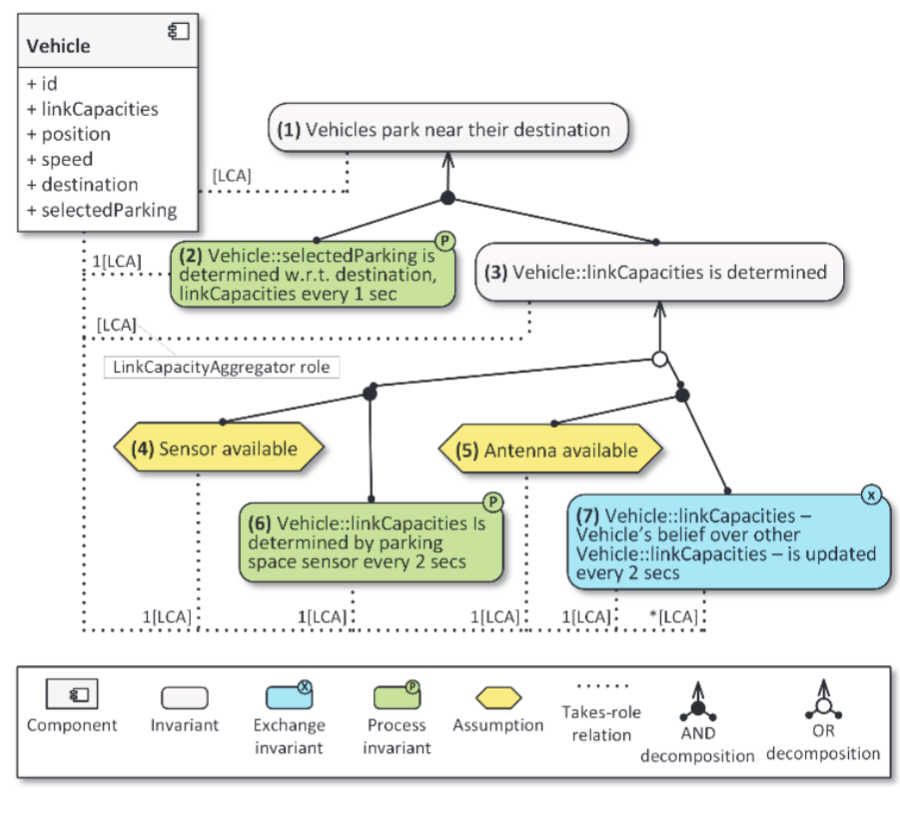
\includegraphics[scale=0.40]{figures/irm}
\caption{IRM tree for a smart parking senario}
\label{fig:irm}
\end{figure}

\subsubsection{Design and Runtime}

Regarding the design and runtime parts \cite{Bures:2013:DEC:2465449.2465462}\cite{AlAli:2014:DEC:2591062.2591140} , the team developed a runtime environment which is implemented in java and is known as jDEECo. The developer is able to design systems that respect the DEECo specification (i.e. SCEL specification), which is captured by specific Java annotations provided by jDEECo runtime Figure~\ref{fig:deeco_code}. More specifically, the designed system consists of roles\uidx{Role}, components\uidx{Component}, and ensembles\uidx{Ensemble}. Each role has a set of attributes, which represent the knowledge related to this specific role. Furthermore, each component is defined as a set of processes\uidx{Process} featuring (a) role(s) having by that the role knowledge besides its local knowledge. Having knowledge in the role allows for preserving the encapsulation of the components\uidx{Component} that features the role and provides a separation in concerns\uidx{Concern}. Hence, each ensemble forms depending on the context and perform knowledge exchange between different components with determined roles. 

\begin{figure}[!h]
\centering
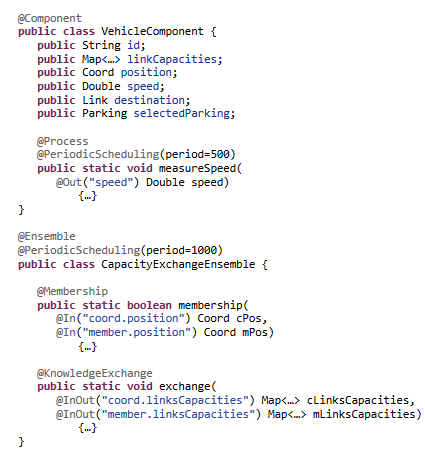
\includegraphics[scale=0.70]{figures/deeco_code}
\caption{Snippet of jDEECo code}
\label{fig:deeco_code}
\end{figure}

\begin{figure}[!h]
\centering
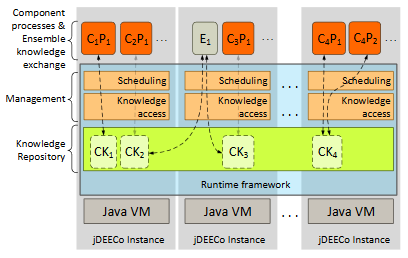
\includegraphics[width=\textwidth]{figures/jdeeco}
\caption{jDEECo runtime framework architecture}
\label{fig:ros}
\end{figure}

 It is worth mentioning that there is another framework that integrates with jDEECo, which is called Intelligent Ensemble framework\footnote{\url{http://d3s.mff.cuni.cz/software/deeco/files/seams-2017.zip} or \url{http://dx.doi.org/10.4230/DARTS.3.1.6}} \cite{Krijt2017Intelligent}. It provides the developer with Ensemble Definition Language (EDL) that was developed using XText and XPand on Eclipse Modelling Framework. At runtime the formation of the ensemble is optimized by using Z3 SMT solver.  
 
\begin{figure}[!h]
\centering
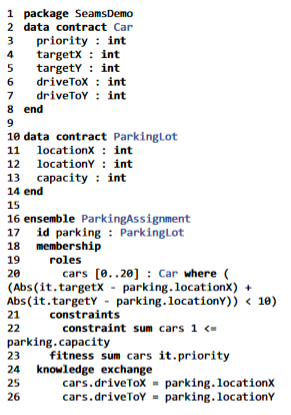
\includegraphics[scale=0.75]{figures/edlspec}
\caption{An example with an EDL specification}
\label{fig:ros}
\end{figure}


\begin{figure}[!h]
\centering
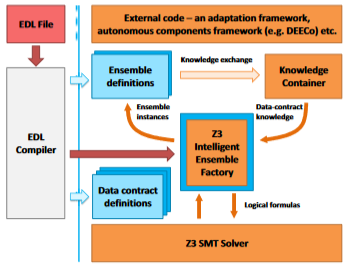
\includegraphics[width=\textwidth]{figures/edl}
\caption{Framework high-level architecture that supports Ensemble Definition Language (EDL)}
\label{fig:ros}
\end{figure}

Not only is DEECo implemented in java, but also it is implemented in C++ \footnote{\url{http://d3s.mff.cuni.cz/projects/components_and_services/deeco/files/CDEECo.zip}} and Scala\footnote{\url{ http://github.com/d3scomp/tcof}}. Nevertheless, the model operations\uidx{ModelOperation} that we mentioned here (i.e. transformation\uidx{TransformationOperation} and integrations\uidx{IntegrationOperation}) are applied on jDEECo (i.e. java implementation).

 
\subsubsection{Self-Adaptation}
Self-adaptation is done in two methods. The first method is by transforming IRM tree to java code with annotations, then at runtime the annotations are processed by IRM-SA engine which uses SAT solver to make decisions between the different paths. The other method is by using modes and mode-switching annotations that are provided by DEECo. It is possible to associate a mode to a set of processes, thus when a mode-switch happens a different set of processes is activated.

There is a part that is presented as an extension of mode-switch transition logic, which are: 1) ordinary differential equation (ODE) to evaluate the inaccuracy\uidx{Accuracy} boundaries of physical attributes~\cite{10.1109/WICSA.2014.20}, 2) statistical testing to use prediction depending on trends of historical data~\cite{7516826}.

Another essential point that DEECo focuses on is forming ensembles and exchanging knowledge. DEECo manifests those concepts and allows for using conditions that are a representation of context to form ensembles. The conditions are refined by using a Z3 SMT Solver~\cite{Krijt2017Intelligent} and fitness, which filter out the less suitable compositions between all possible ones. Regarding exchanging knowledge between components\uidx{Component}, it could be determined by context constraints\uidx{Constraint} or by adding boundaries on gossip protocol that is responsible of spreading information~\cite{Bures2014}. Furthermore, DEECo allows a hierarchical composition for ensembles~\cite{Bures:2015:TIE:2797433.2797450}\cite{Bures2016}.

\begin{figure}[!htb]
\centering
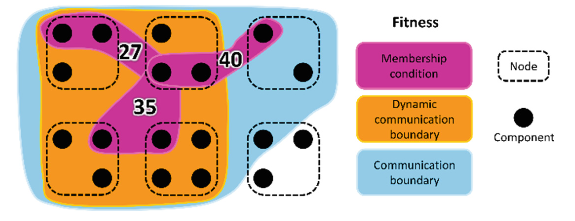
\includegraphics[scale=0.60]{figures/fitness}
\caption{Membership vs. boundary conditions in ensemble formation}
\label{fig:fitness}
\end{figure}

\subsubsection{Simulation}
Finally, the simulation part targets two domains for vehicles\cite{Kit:2015:AFE:2821357.2821374} and robots\cite{Matena:2016:MPT:2897053.2897065}. Concerning vehicles, jDEECo has an integration with MATSim which allows to simulate vehicles and OMNET++ which simulates the network delays. Regarding the robots case, jDEECo has an integration with ROS which simulates movements of robots. While ROS has in its turn an integration with OMNET++ to simulate network delays and with Stage to simulate sensors and actuators.

\begin{figure}[!htb]
\centering
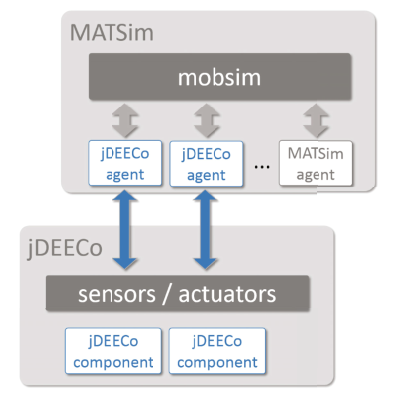
\includegraphics[scale=0.55]{figures/matsim}
\caption{jDEECo integration with MATSim}
\label{fig:matsim}
\end{figure}

\begin{figure}[!htb]
\centering
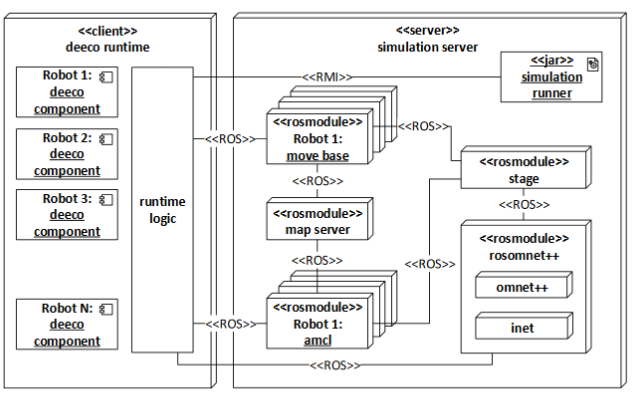
\includegraphics[scale=0.65]{figures/ros}
\caption{jDEECo integration with ROS}
\label{fig:ros}
\end{figure}


 To conclude, DEECo development environment provides a toolchain for modeling CPS system with an emergent behavior\uidx{BehaviouralCharacteristic} starting from requirement to runtime and simulation. To get the different views of system developmen,t many transformation and integration operations\uidx{IntegrationOperation} are involved which supports the idea of multi-paradigm modeling\uidx{Paradigm}. These are further presented in the developed ontology of DEECo briefly presented below.
 
 
 
\subsubsection{Applications}
%\STATUS{descriptions of presented use cases in different domains}
  Many applications were introduced using DEECo concepts, which are in Automotive, Robotics, Clouds and Industry domains. 
 
 The Automotive example \cite{Hoch2015emobi} is basically to present aspects of requirements, self-adaptation, networking, and simulation. The IRM tree represents finding a free parking and MATSim \footnote{\url{https://matsim.org}} simulates the traffic. The models involved in this example are IRM Model, DEECo Design time Model, DEECo Runtime Model, and MATSim. Furthermore, in  \cite{Kit2015empl}, the example presents road trains that use MANETs network and utilizes the knowledge exchange by using bounded gossiping \cite{10.1007/978-3-319-09970-5_23}.

\begin{figure}[!htb]
\centering
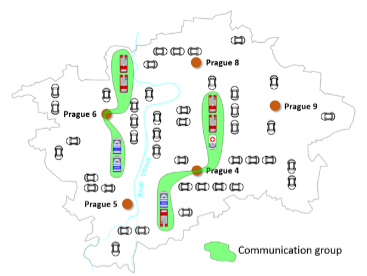
\includegraphics[width = \textwidth]{figures/gossip}
\caption{Illustration of communication\uidx{Communication} groups; each is associated with an instance of SameDestination}
\label{fig:gossip}
\end{figure}

Also, a railroad emergency response service example includes trucks helping damaged trains (e.g. because of low fuel quality) \cite{modelsward17}. The service should take into account the performance and the balance in serving between different clients. In other words, repairing the trains should be fast, but also the trucks should consider the situation in case another farther train was damaged at the same time (i.e. not only going to the closest train). Here, the development starts with defining EDL Files, compiling them, and then generating the DEECo Design time Model. At runtime, the DEECo Runtime Model integrates with Z3 SMT Solver to optimize forming the ensembles.

\begin{figure}[!htb]
\centering
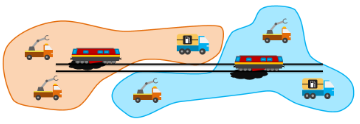
\includegraphics[scale=0.85]{figures/trains}
\caption{Example of two well-chosen emergency groups.}
\label{fig:trains}
\end{figure}

The FireFighter Coordination example is another example that represents the use of IRM-SA model and DEECo \cite{Gerostathopoulos:2017:SAC:3068423.2823345} \cite{GEROSTATHOPOULOS2016378}. The example describes groups of firefighters that have to operate using low-power nodes and without communication guarantees. The work presents self-adaptation using multi-layered architecture\uidx{Architecture}, which are: Meta-Adaptation Layer, Adaptation Layer,and Business System. Thus, the example involves IRM-SA model, Self-Adaptation Model, DEECo Runtime Model and DEECo Design time Model.
 
 Another example related to parking places but with edge cloud usage is presented in ~\cite{Bures:2018:PMS:3185768.3186306} Figure \ref{fig:parking}. The example describes vehicles that detect parking spots and informs other vehicles about it. The used simulation tool is Veins LTE, which is based on OMNeT++\footnote{\url{https://www.omnetpp.org}} (i.e. network simulator), INET\footnote{\url{https://inet.omnetpp.org}} and SimuLTE\footnote{\url{http://simulte.com}} (i.e. radio simulators), and SUMO\footnote{\url{http://sumo.dlr.de}} (i.e. road traffic simulator). The main concern\uidx{Concern} is performance model that is presented by Queueing Networks (QN), and it is planned to be integrated with DEECo. 
 
\begin{figure}[!htb]
\centering
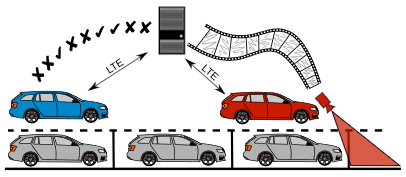
\includegraphics[scale=0.65]{figures/parking}
\caption{Scanning cars (on the right) are sending a photo stream to the edge cloud server reporting spot availability to the parking cars (on the left)}
\label{fig:parking}
\end{figure}
 
Regarding Clouds domain, the example concerns are performance and adaptation, and targets real-time guarantees for image processing application that runs on edge-cloud architecture [\cite{Hnetynka:2018:GLA:3241403.3241448}]. The work is in progress and it will involve Statistical Model with Self-Adaptation Model from the current models. 

As for predictability\uidx{Predictability} and adaptability\uidx{Adaptability}, the use case present cleaners that detect the need for charging or cleaning, and the active mode is determined statistically to avoid premature mode-switch \cite{bures2016stat}. This example involves the statistical mode-switching in Self-Adaptation Model, in addition to DEECo Design time Model and DEECo Runtime Model. The evaluation of statistical functions was done on STM32F4-DISCOVERY board. 
 
 \begin{figure}[!htb]
\centering
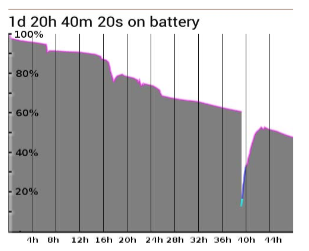
\includegraphics[scale=0.65]{figures/statistical}
\caption{Sample battery energy level during continuous discharge }
\label{fig:statistical}
\end{figure}

 
 Another case is Autonomous Cleaning  Robots  Coordination (ACRC) \cite{Matena2016Model} where robots have tasks of visiting and cleaning the offices. The problems that robots encounter here are imprecise localization, limited communication range, and latencies, which are solved by introducing self-healing in the self-adaptation logic. The testbed is done using ROS simulation for robots with camera (i.e. Stage) for navigation and IEEE 802.15.4 transceiver for communication (i.e. OMNet++). \footnote{\url{http://d3s.mff.cuni.cz/projects/components_and_services/deeco/files/seams-2016-artifact.zip}}
 
 \begin{figure}[!htb]
\centering
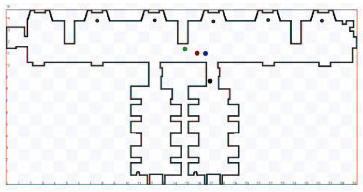
\includegraphics[scale=0.65]{figures/robots}
\caption{A visualization of the the area that cleaners should visit and clean}
\label{fig:robots}
\end{figure}

The scalability\uidx{Scalability} issue was targeted in an example about intelligent production line (IPL) \footnote{\url{https://github.com/d3scomp/scalable-reliability}} \cite{Matena2017enssca}. The example also aims at preserving the safety\uidx{Safety} conditions in the work place with taking into account the scalabe QoS grantees. To put it differently, the robots have safety zone and speed grantees, which change depending on the number of human and robots in the area. The used models are OMNeT++ and INET simulators with DEECo Design Model and DEECo Runtime Model.
\begin{figure}[!htb]
\centering
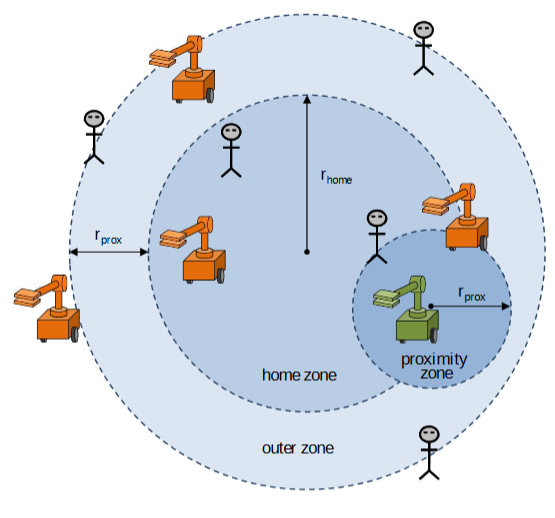
\includegraphics[scale=0.50]{figures/productionline}
\caption{Intelligent production line: home, proximity, and outer zones}
\label{fig:productionline}
\end{figure}

 The privacy and trust use case describes the exchange of the sensitive data between companies or inside the company itself \cite{Al-Ali:2018:MDT:3241403.3241450},\cite{10.1007/978-3-030-03424-5_12},\cite{alali2018usecases} (i.e. as part of Trust 4.0 project\footnote{\url{http://trust40.ipd.kit.edu/home/}}). More specifically, the system preserves information by preventing physical encounter between different teams, which is done through granting/denying access for the employees depending on the time table and existing people in the room \cite{10.1007/978-3-030-03424-5_12}. Another example is about production shifts, the foreman role has access only for employees' names in that shift. In case the system detects a possible delay of one of the employees, the system grants the foreman an access to name and phone number of a backup employee. Similarly, the confidentiality\uidx{Confidentiality} levels between companies depends on the context such as encountering incidents. These examples uses the basic concepts of DEECo (i.e. DEECo Design time Model and DEECo Runtime Model) in Scala \footnote{\url{https://www.scala-lang.org/}}. It involves fitness model in the lunch room example \cite{10.1007/978-3-030-03424-5_12}, and ValueStreamer \footnote{\url{https://www.valuestreamer.de/en/home/}} and PCM \footnote{\url{https://www.palladio-simulator.com/science/palladio_component_model/}} on industry 4.0 example.   
 
\begin{figure}[!htb]
\centering
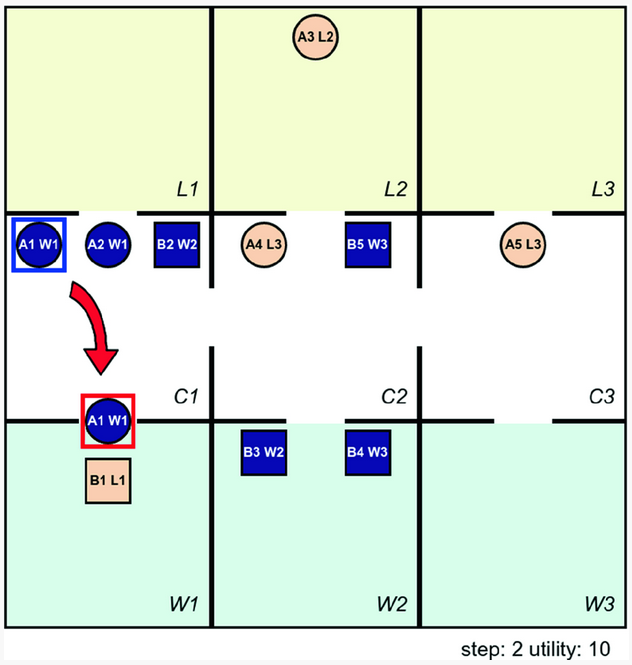
\includegraphics[scale=0.44]{figures/lunchroom}
\caption{Entry for the developer A1 to room W1 is rejected due to the presence of the developer B1}
\label{fig:lunchroom}
\end{figure}

  
 \begin{figure}[!htb]
\centering
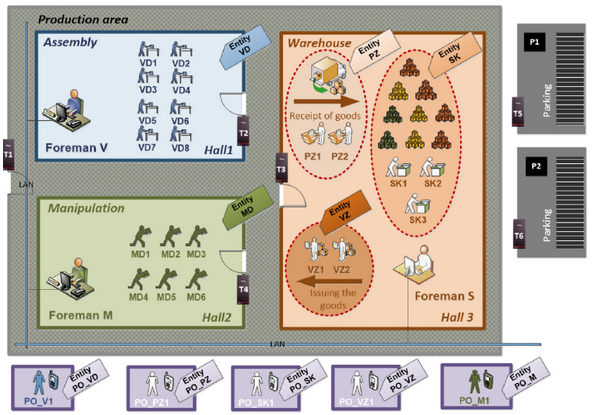
\includegraphics[scale=0.70]{figures/shifts}
\caption{The use case illustrates a production area, which has many halls. For each hall, there is a single foreman who manages the workers.}
\label{fig:shifts}
\end{figure}
 
\subsection{Ontology}
 The structure\uidx{StructureCharacteristic} of DEECo is described using the ontologies provided by MPM4CPS. This is done by instantiating its classes, so the created set of individuals represents DEECo.
 
 \subsubsection{CPS}
% \STATUS{ready for review}
In order to present all the related parts in the example, we refer to the tasks related to vehicle joining a road train as (1), and vehicle finding a parking slot as (2).

\begin{itemize}
    \item \checkmark \textbf{ConstituentElement} : (mandatory) The elements constituting the system
    \begin{itemize}
        \item \checkmark \textbf{Cyber}: (mandatory) System model based on DEECo concepts.
        \begin{itemize}
            \item \checkmark \textbf{Software}: Collection of data or computer instructions that tell the computer/controller of the robot, how to work. 
            \begin{itemize}
                \item \checkmark \textbf{Application Software}: The simulation software used to simulate traffic conditions and the EBCPS.
                \item \checkmark \textbf{System Software}: The system software is the software running on the simulation computer and all of its included \textbf{System Services} and \textbf{System Utilities}.
                \item \xmark \textbf{Embedded Software (Firmware)} 
            \end{itemize}
        \end{itemize}
        \item \checkmark \textbf{Control}: (mandatory) (1)(2) Vehicles have PID controllers to maintain the desired speed and the desired distance based on the driver preferences or the determined values in each vehicle mode in addition to (2) heading to the destination. 
        \begin{itemize}
            \item \checkmark \textbf{State}: We determine the states, which are the operational modes, of (1) a vehicle in a road train to be "Cooperative Adaptive Cruise Control (CACC)" or "Adaptive Cruise Control (ACC)", and of (2) a vehicle parks in a city to be "waiting", "search for parking lot", "reserve parking slot", "cancel reserved parking slot", "parking slot reserved", "search for parking slot on spot", "find parking slot on spot", "parking", "parked", or "leave the parking slot". The (2) parking lot has the following states for each parking slot: "available", "reserved", "canceled", "filled".  
            \item \checkmark \textbf{Disturbance}: (1)(2) Noise in sensors measurements, (1)(2) communication problems, and (1) traffic fluctuation.
            \item \checkmark \textbf{Input}: (1) In road train, the vehicle receives the speed and the position of the vehicle in front. (2) Regarding finding a parking slot, the input is the availability of the parking lots, the available slots detected by other vehicles, 
            \item \checkmark \textbf{Output}: (2) In road train, the vehicle speed and distance from the vehicle in front is maintained. (2) When reaching the parking slot, the vehicle parks.
            \item \checkmark \textbf{Goal}: (1) Hard real-time goal keep a save distance, (1) Soft real-time goal save fuel, and (2) Soft real-time goal is parking.
            \begin{itemize}
                \item \checkmark \textbf{Setpoint}: (1) The desired speed and the desired distance from the vehicle in front. (2) The final destination and the parking stops in between for the vehicle.
                \item \checkmark \textbf{Tracking}: The vehicle checks for the driver's inputs for (1) the desired speed and (1)(2) the desired stops, or (1) updates from the vehicles in the road train for the speed and distance to maintain. (2) The vehicle receives information about available parking slots from other vehicles or from parking lots. 
                The \textbf{ValidityRegion} of the tracking in (1) the vehicle is local when vehicle is not in a road train and decentralized when vehicle is in a road train. Additionally, (2) the vehicle tracks the available parking slots in decentralized manner. The \textbf{ValidityRegion} of the tracking in (2) the parking lot functions in decentralized manner. 
                \item \checkmark \textbf{Regulation}: (1)(2) The vehicles communicate with each other to maintain the road train or to find an available parking slots on the spot. (2) The vehicle communicates with the parking lot to reserve a parking slot.  
                \item \checkmark\  \textbf{Reference Signal}: (1)(2) The GPS signal is a reference signal in vehicles for self-positioning and (2) calculating the distance from the stops and parking lots.
            \end{itemize}
            \item \checkmark \textbf{Feedback}: (1) There are two kinds of feedback loops in the autonomous vehicle. The first is part of the control loop to regulate the speed and the safety distance. We represent that loop using MAPE-K model~\cite{Sinreich2006AnAB}. The second feedback learns about the vehicle behavior and the reliability of the sensors to perform better adaptation.
            \begin{itemize}
                \item \checkmark\textbf{Dependency}: (1) The first feedback for the system is the measured acceleration from vehicle accelerometer (i.e. output of the Plant), which feeds back into the PID controller. The second feedback is studying the vehicle behavior and the reliability of the sensors to decide adapting to a more suitable mode for the current situation (e.g. change from CACC to ACC in case the wifi communication is unreliable). 
                \item \checkmark\textbf{Scope}: (1) The scope of the control signals is local to the vehicle.
            \end{itemize}
            \item \checkmark\textbf{Dynamics} Context-based ensembles i.e. The vehicles can form in dynamic groups to (1) maintain distance in a road train or (2) detect available parking slots, and (2) the vehicles form a dynamic grouping with the parking lots to exchange information about the parking slots. 
            \begin{itemize}
                \item \checkmark \textbf{SystemType}: (\textbf{Linearity}) (1) The vehicle movement is non-linear. (\textbf{Time}) The system is discrete with relation to (1) the control-loop in the vehicle and the communication with (1)(2) other vehicles or (2) the parking lots.. (\textbf{Continuity}) The vehicle movement is continuous in reality. However, in the simulation it is discretized. 
                \item \textbf{Behaviour} (\textbf{Equilibria}) There exist multiple \textbf{Distributed} equilibria for each car. The \textbf{(Emergent Behavior)} of the CPS. 
                \item \textbf{Topology} (\textbf{Evolution}) (1)(2) The connections between the components are dynamic over time (i.e. through ensembles), which (\textbf{Implementation}) support adding constraints over the connections that provide context-awareness into the system.
            \end{itemize}
            \item \checkmark \textbf{Properties}: Autonomy, adaptation, learning and uncertainty. (\textbf{Uncertainty}) In the example, we consider white noise in measurements and network delays (i.e. stochastic and exponential distribution accordingly).
            \item \xmark\ \textbf{Diagnostics}: No automatic diagnostic. 
            \item \checkmark \textbf{Prognostics}: The prediction is used in the system in the adaptation decision. For instance, after learning the vehicle behavior, (1) the vehicle decide to change mode to ACC because the WiFi communication is unreliable. 
        \end{itemize}
        \item \checkmark \textbf{Human}: The driver determine the next tasks to be performed in the vehicle.
        \begin{itemize}
            \item \checkmark \textbf{Role}: (1) The driver decide to join or leave a road train, and (2) determine the final destination of the trip and the stops in between.
            \item \checkmark \textbf{Event}: (1) Detecting a road train, (2) Determine the locations to visit. 
            \item \textbf{Entity}: The driver.
            \item \checkmark \textbf{Action}: the driver can make a (1) Request for joining or leaving a road train, or a (2) Request for finding a parking slot. 
        \end{itemize}
        \item \checkmark \textbf{Network}: (mandatory) The communication is Peer-to-Peer communication (i.e. MANET-based wireless and IP-based communication)
        \begin{itemize}
            \item \checkmark \textbf{Configuration}: (mandatory) The communication of peer-to-peer communication. % , gossip-based communication.
            \item \checkmark \textbf{Communication}: (mandatory) The communication is governed by protocols and constraints.
            \begin{itemize}
                \item \checkmark \textbf{ComType}: %\rima{I am not sure from the options here?}
                (mandatory) asynchronous communication since the communication is implicit, where the components propagate their knowledge and do not wait for an answer. However, we assume a shared clock for all the components in the example.
                \item \checkmark \textbf{Protocol}: (mandatory) Gossiping via (2) UDP on top of Ethernet NIC and (1)(2) broadcast via wireless NIC.  
            \end{itemize}
        \end{itemize}
        \item \checkmark \textbf{Physical}: (mandatory) The physical elements of the vehicle, the parking lots.
        \begin{itemize}
            \item \checkmark \textbf{Sensor}: (mandatory) (1) When vehicle is on the road the used sensors are: wifi antenna, GPS antenna, camera, radar, lidar, ultrasonic, and accelerometer. (2) When the vehicle is looking for parking the camera in the vehicles, and (2) camera or sensors in the parking lots to detect the availability of a parking slot.  
            \item \checkmark \textbf{Actuator}: (mandatory) In the vehicle (1) the gas and brake pedals (i.e. vehicle engine). Even though the publications did not cover the automatic parking , however it is interesting to highlight the (2) steering as actuators in the vehicle.
            \item \checkmark \textbf{Plant}: (mandatory) (1) The vehicle movement equations (because we simulate)
            \item \checkmark \textbf{Controller}: (mandatory) (1) The PID controllers
            \begin{itemize}
                \item \xmark \textbf{Mechanical}
                \item \checkmark \textbf{Hardware Platform}: Consists of \textbf{Processor}, \textbf{Memory}, \textbf{System Bus}, \textbf{Hardware Topology}, and \textbf{Application-specific Circuit}
            \end{itemize}
            \item \checkmark \textbf{Environment}: (mandatory) (2) The cities, and (1)(2) the roads. 
        \end{itemize}
    \end{itemize}
    \item \checkmark \textbf{nonfunctionalReqs} :  Safety, Efficiency, Adaptability
    \item \checkmark \textbf{ApplicationDomain} :  Transportation
    \item \checkmark \textbf{Disciplines} : The disciplines associated with the vehicle are - \textbf{Software Engineering} and \textbf{Mechanical Engineering} 
\end{itemize}
 

 \subsubsection{MPM}
% \STATUS{ready for review}
  In this part, the individuals includes a DEECo megamodel\uidx{Megamodel} and its fragments\uidx{MegamodelFragment} defining all model operations\uidx{ModelOperation} supported by DEECo as outlined in Figure~\ref{fig:deeco_map} and Figure~\ref{fig:deeco_ontology}. Model operations\uidx{ModelOperation} are of different kinds such as transformation and integrations operations\uidx{IntegrationOperation}. The first model operation is the capture of requirements followed by a transformation operation\uidx{TransformationOperation} from the requirements model into a design model, then by an instantiation operation to create runtime model and simulation model. The runtime model integrates with the self-adaptation model Figure~\ref{fig:deeco_tools}.

\begin{figure}[!htb]
\centering
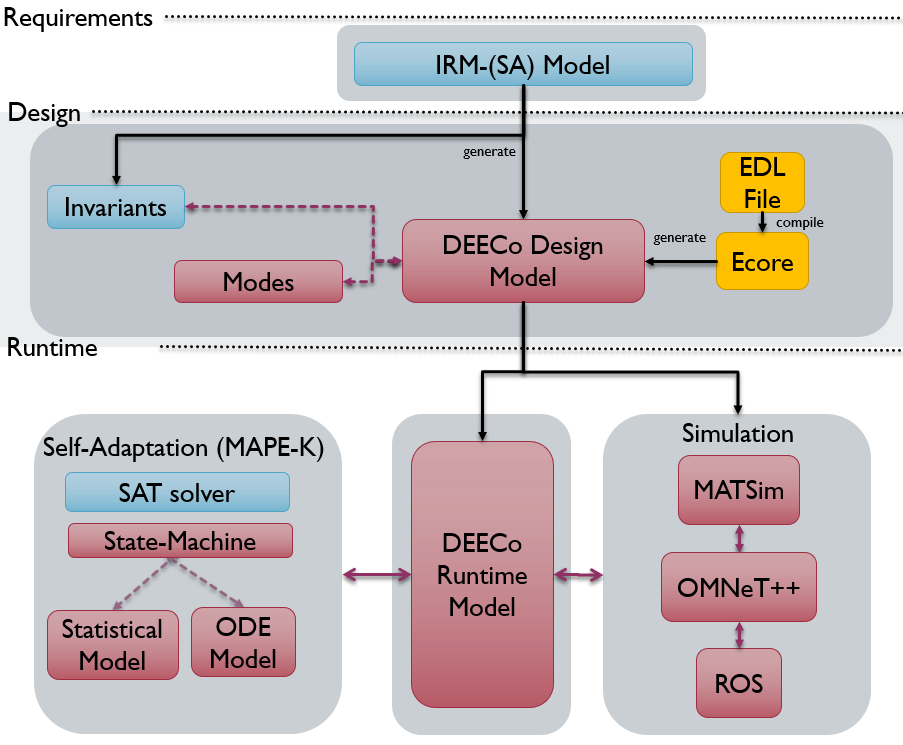
\includegraphics[scale=0.50]{figures/deeco_tools_adv.PNG}
\caption{Models and Tools Transformations and integrations}
\label{fig:deeco_tools}
\end{figure}

\begin{figure}[!h]
\centering
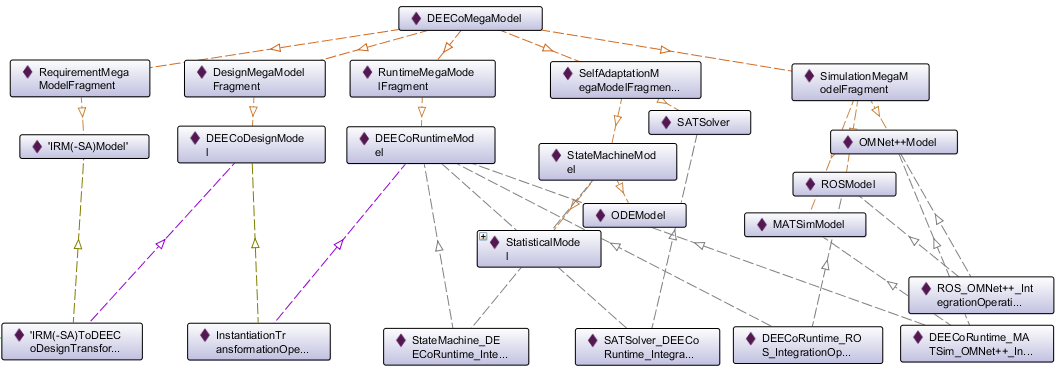
\includegraphics[scale=0.55]{figures/ontology.PNG}
\caption{The example of DEECo represented by OntoGraf using Protege}
\label{fig:deeco_ontology}
\end{figure}

\subsubsubsection{\textbf{Formalism, Models, and Tools}}

\begin{itemize}
    \item \uidxp{Formalism}
        \subitem \uidxp{AutomataBasedFormalism}: LTS (Labeled Transition System)
    \item Language
        \subitem \uidxp{FormalLanguage}: SCEL (Service Component Ensemble Language)
        \subitem \uidxp{ArchitecturalDescriptionLanguage}: DEECo realizes SCEL
        \subitem \uidxp{ModelingLanguage}: IRM, IRM-SA 
 %       \subitem ProgrammingLanguages: Java
 %       \subitem TransformationLanguages: Epsilon 
    \item Model
        \subitem MegaModel: DEECo (DEECo stands for Dependable Emergent Ensembles of Components)
        \subitem MegaModelFragment: \textit{mentioned below in details}
    \item ModelRelation: \textit{mentioned below in details}
    \item Tool
        \subitem ModelingTool: IRM-SA (Invariant Refinement Method - Self-Adaptation) developed in D3S Charles University in Prague, EclipseEpsilon
        \subitem RuntimeTool: jDEECo from Department of Distributed and Dependable Systems, Charles University in Prague
        \subitem SimulationTool: ROS from Open Source Robotics Foundation, OMNet++ from OpenSim Ltd,  MATSim from MATSim Community %, Stage from Richard Vaughan and contributors 1998-2011 Part of the Player Project
\end{itemize}


\subsubsubsection{\textbf{MegaModel Fragments / Models for DEECo}}
\begin{itemize}
    \item Requirements MegaModel Fragment\uidx{MegamodelFragment}
        \subitem Models: IRM Model 
    \item Design MegaModel Fragment
        \subitem Models: DEECo Design Model 
    \item Self-Adaptation MegaModel Fragment
        \subitem Models: IRM-SA Model, Mode-Switching Model 
    \item Runtime MegaModel Fragment
        \subitem Models: DEECo Runtime Model
    \item Simulation MegaModel Fragment
        \subitem Models: MATSim, ROS, OMNET++ %, Stage 
\end{itemize}


\subsubsubsection{\textbf{Tools / Model Operations for DEECo}}
\begin{itemize}
    \item Model Operation\uidx{ModelOperation}: Requirements Capturing Operation\uidx{CapturingOperation} - Modeling requirements refinements by Human
        \subitem Input: Human 
        \subitem Output Model(s): IRM-SA Model
        
    \item Model Operation\uidx{ModelOperation}: Requirements-Design Transformation Operation\uidx{TransformationOperation} - Capturing requirements refinements in design time
        \subitem Input Model(s): IRM-SA Model
        \subitem Output Model(s): DEECo Design Model 
        
   \item  Model Operation\uidx{ModelOperation}: Instantiation-Transformation Operation\uidx{TransformationOperation} - Instantiation of the DEECo components and ensembles 
        \subitem Input Model(s): DEECo Design Model
        \subitem Output Model(s): DEECo Runtime Model
        
   \item  Model Operation\uidx{ModelOperation}: Instantiation-Transformation Operation2\uidx{TransformationOperation} - Instantiation of the Simulation Model 
        \subitem Input Model(s): DEECo Design Model
        \subitem Output Model(s): ROS, MATSim , OMNet++ 

    \item Model Operation\uidx{ModelOperation}: Runtime-to-Vehicle Simulation Integration Operation\uidx{IntegrationOperation} - System Design Validation
        \subitem Input Model(s): DEECo Runtime Model
        \subitem Output Model(s): MATSim , OMNet++ 
        
    \item Model Operation\uidx{ModelOperation}: Runtime-to-Robot Simulation Integration Operation\uidx{IntegrationOperation} - System Design Validation
        \subitem Input Model(s): DEECo Runtime Model
        \subitem Output Model(s): ROS 
        
    \item Model Operation\uidx{ModelOperation}: Simulation-to-Simulation Integration Operation\uidx{IntegrationOperation} - System Design Validation
        \subitem Input Model(s): ROS
        \subitem Output Model(s): OMNet++ %, Stage 
    
\end{itemize}

 \subsubsubsection{\textbf{Development Process}}

The development process\uidx{Process} starts with capturing requirements operation in which a human is responsible of defining the IRM-SA model. Afterwards, the IRM tree is transformed to DEECo Design Model, which its instantiation are DEECo Runtime Model and Simulation Models. 

The DEECo Runtime Model is integrated with self-Adaptation model. It is possible also to define modes and their transitions in DEECo Design time model. Hence, the logic over transitions are extensible with ODE or statistical reasoning. Similarly, it is possible to define in the DEECo Design Model formation of ensembles by using gossiping boundary and fitness. The boundary defines limits on gossiping protocol and the fitness evaluates the history of forming ensembles and select the best fitting group of components that are involved to form the ensemble.

Finally, DEECo Runtime Model is also integrated with simulation models. For more information, please check the following links:
\begin{itemize}
    \item DEECO website: \url{http://d3s.mff.cuni.cz/software/deeco/}
    \item jDEECo: https://github.com/d3scomp/JDEECo/tree/simulation
    \item IRM: \url{http://d3s.mff.cuni.cz/software/irm/}
    \item Modes: \url{https://github.com/d3scomp/JDEECo/tree/master/jdeeco-modes}
    \item Statistical Operations: \url{https://github.com/d3scomp/TimeSeriesStatistics}
    \item OMNet++: \url{http://d3s.mff.cuni.cz/projects/components_and_services/deeco/files/jDEECo-OMNeT.zip}
    \item MATSim: \url{http://d3s.mff.cuni.cz/projects/components_and_services/deeco/files/jDEECo-MATSim.zip}
    \item ROS: \url{http://d3s.mff.cuni.cz/projects/components_and_services/deeco/files/seams-2016-artifact.zip}
    \item Intelligent Ensemble framework: \url{http://d3s.mff.cuni.cz/software/deeco/files/seams-2017.zip}
\end{itemize}


\subsubsection{MPM4CPS}
In this part, the views\uidx{View} and viewpoints\uidx{ViewPoint} for this system are described as following:

\begin{itemize}
 
    \item View\uidx{View}: Requirement Designer
    \item ViewPoint\uidx{ViewPoint}: The concerns\uidx{Concern} in this viewpoint is related to resilience\uidx{Resilience}, and involves both roles and ensembles in the system. The designer determines the environmental assumptions to each choice to ensure preserving the required invariants. That makes this viewpoint related to the cyber part of the system\uidx{SystemPart} (i.e. software).
    
    \item View\uidx{View}: Component Designer
    \item ViewPoint\uidx{ViewPoint}: The concerns\uidx{Concern} in this viewpoint is related to performances, accuracy\uidx{Accuracy}, robustness\uidx{Robustness} and self-adaptation. It involves designing roles\uidx{Role}, processes\uidx{Process} and modes\uidx{Mode}, in addition to relations\uidx{Relation} between processes and the assumptions from requirement phase. Also, components contain controllers, sensors, and actuators, which means that this viewpoint is related to physical and cyber parts of the system\uidx{SystemPart}.   
    
    \item View\uidx{View}: Ensemble Designer
    \item ViewPoint\uidx{ViewPoint}: The concerns in this viewpoint are related to knowledge exchange, security\uidx{Security}, optimization, scalability\uidx{Scalability} and performances. The designer should determine the roles\uidx{Role} involved in ensembles, the context constraints and what information to exchange. Additionally, the designer can optimize forming the ensembles by using fitting function and defining a boundary over gossip protocol. The design of ensembles could be also associated to system requirements as it is mentioned in the Requirement Designer view. This makes this viewpoint related to network and cyber (i.e. software) parts of the system\uidx{SystemPart}.
    
\end{itemize}


%%%%%%%%%%%%%%%%%%%%%%%%%%%%%%%%%%%%%%%%%%%%%%%%%%%%%%%%%%%%%%%%%%%%%%%%%%%%%%%%%%%%%%%%%%%%%%%%%%%
% CPS 
%%%%%%%%%%%%%%%%%%%%%%%%%%%%%%%%%%%%%%%%%%%%%%%%%%%%%%%%%%%%%%%%%%%%%%%%%%%%%%%%%%%%%%%%%%%%%%%%%%%

%%%%%%%%%%%%%%%%%%%%%%%%%%%%%%%%%
% Elements  % STKLIK: comment the next two lines, because of "command already defined" error
% \newcommand{\CPSCyberPart}{\p{CyberPart}\xspace}
% \newcommand{\CPSPhysicalPart}{\p{PhysicalPart}\xspace}

%%%%%%%%%%%%%%%%%%%%%%%%%%%%%%%%%%%%%%%%%%%%%%%%%%%%%%%%%%%%%%%%%%%%%%%%%%%%%%%%%%%%%%%%%%%%%%%%%%%
% MPM 
%%%%%%%%%%%%%%%%%%%%%%%%%%%%%%%%%%%%%%%%%%%%%%%%%%%%%%%%%%%%%%%%%%%%%%%%%%%%%%%%%%%%%%%%%%%%%%%%%%%


%%%%%%%%%%%%%%%%%%%%%%%%%%%%%%%%%
% MegaModel
\newcommand{\CPSLabMM}{\p{CPSLabMM}\xspace}

% MegaModelFragments
\newcommand{\CPSLabMTMMF}{\p{CPSLabMTMMF}\xspace}
\newcommand{\CPSLabMiLMMF}{\p{CPSLabMiLMMF}\xspace}
\newcommand{\CPSLabRPaMMF}{\p{CPSLabRPaMMF}\xspace}
\newcommand{\CPSLabRPbMMF}{\p{CPSLabRPbMMF}\xspace}
\newcommand{\CPSLabSiLaMMF}{\p{CPSLabSiLaMMF}\xspace}
\newcommand{\CPSLabSiLbMMF}{\p{CPSLabSiLbMMF}\xspace}
\newcommand{\CPSLabHiLMMF}{\p{CPSLabHiLMMF}\xspace}

% Languages
\newcommand{\MATLABSimulinkLanguage}{\p{MATLAB/Simulink Language}\xspace}
\newcommand{\FESTORobotinoSimLanguage}{\p{FESTO Robotino{\copyright}Sim Language}\xspace}
\newcommand{\AUTOSARLanguage}{\p{AUTOSAR Language}\xspace}


% Models
\newcommand{\CPSLabControlModel}{\p{ControlModel}\xspace}
\newcommand{\CPSLabControlModelCode}{\p{ControlCode}\xspace}
\newcommand{\CPSLabPlantModel}{\p{PlantModel}\xspace}
\newcommand{\CPSLabRobotModel}{\p{RobotModel}\xspace}
\newcommand{\CPSLabSystemModel}{\p{SystemModel}\xspace}
\newcommand{\CPSLabSystemModelCode}{\p{SystemCode}\xspace}
\newcommand{\CPSLabSystemModels}{multiple {\CPSLabControlModel}s and one \CPSLabSystemModel\xspace}

% Tools
\newcommand{\MATLABSimulinkEditor}{\p{MATLAB/Simulink Editor}\xspace}
\newcommand{\MATLABSimulinkSimulator}{\p{MATLAB/Stateflow Simulator}\xspace}
\newcommand{\dSPACETargetLink}{\p{dSPACE TargetLink}\xspace}
\newcommand{\dSPACESystemDesk}{\p{dSPACE SystemDesk}\xspace}
\newcommand{\FESTORobotinoSim}{\p{FESTO Robotino{\copyright}Sim}\xspace}
\newcommand{\FESTORobotinoView}{\p{FESTO Robotino{\copyright}View}\xspace}
\newcommand{\DesktopExecution}{\p{Execution on a Desktop computer}\xspace}
\newcommand{\RobotExecutionLocal}{\p{Local execution on a Robotino Robot}\xspace}
\newcommand{\RobotExecutionRemote}{\p{Remote execution on a Robotino Robot}\xspace}


% =====================================================
\addtocounter{footnote}{1}
\section{HPI CPSLab$^{\thefootnote{}}$}\footnotetext[\thefootnote{}]{Acknowledgements: We thank Sebastian W{\"a}tzoldt, Stefan Neumann, Joachim H{\"a}nsel, and Falk Benke for their contributions to the lab described in this section and their contribution to the presented content and figures.}

%\LEAD{Soumyadip}\ALSO{Holger, Dominique}\STATUS{%
%Soumyadip has added some figures from the Pisa keynote and the BX/MX Dagstuhl seminar; 
%Holger restructured the text to reflect the three stages of the ontology; 
%Holger added mappings to the ontologies; 
%STILL TO BE DONE: 
%model the introduced ontology elements in the catalog or CPSLab ontology; 
%add graphics showing the added concepts/instances of the ontologies
%}

To structure the presentation of this case study according to the efforts for the MPM4CPS project, we will
%
at first in Section~\ref{subsec:cpslab-overview} provide an overview about the case study and lab,
%
then in Section~\ref{subsec:cpslab-cps} review the technical setting and derive the required needs concerning the CPS ontology,
%
thereafter in Section~\ref{subsec:cpslab-mpm} we will outline how the models, tools, and tool chain employed in the case study can be captured as multi-paradigm modeling and derive the required needs concerning the MPM ontology, and
%
finally in Section~\ref{subsec:cpslab-mpm4cps} we discuss how the CPS character of the case study is reflected in its multi-paradigm modeling and the use of the MPM4CPS ontology.

% ========================================================================================
\subsection{Overview}\label{subsec:cpslab-overview}


As outlined in more details from a conceptual point of view\uidx{ViewPoint} in \cite{Waetzoldt:2012pa}, the presented \emph{CPSLab}\footnote{http://www.cpslab.de} at the Hasso Plattner Institute (HPI)\footnote{http://www.hpi.de} at the University of Potsdam applied, adapted, and evaluated an existing industrial-strength development methodology from the automotive domain \cite{Broekman&Notenboom2003} (see also Figure~\ref{fig:methodology}) for the robotic system application domain\uidx{ApplicationDomain}. We therefore evaluated and adapted a component-based\uidx{Component} approach using an MDE approach supporting the combination of soft and hard real-time behavior\uidx{BehaviouralCharacteristic}.

\begin{figure}[!htb]
\centering
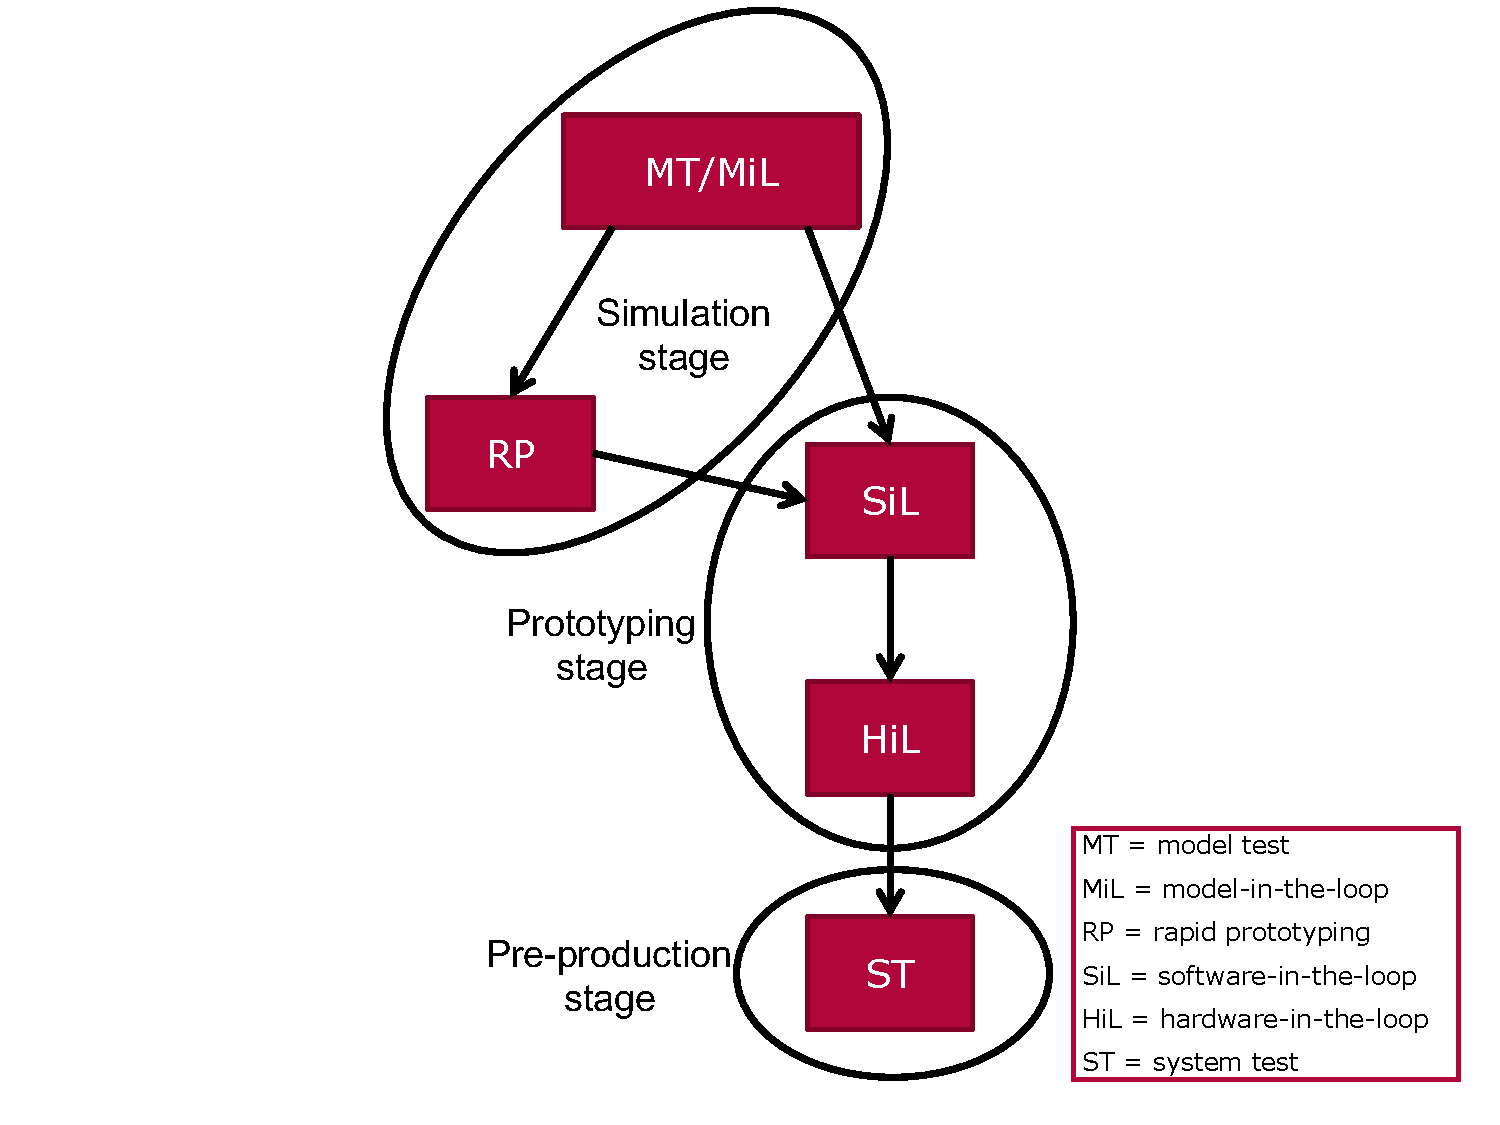
\includegraphics[width=0.66\textwidth]{figures/methodology.pdf}
\caption{Overview of the methodology for modeling, verification, and validation employing simulation and testing (see \cite{Broekman&Notenboom2003})}
\label{fig:methodology}
\end{figure}

The resulting methodology for robotic systems supports several development activities such as modeling, simulation, verification/testing at different stages, prototyping and pre-production. The lab supports tools and related libraries in an integrated tool-chain that reflects physical and cyber aspects of distributed\uidx{Distributed} robotics systems.

\begin{figure}[!htb]
\centering
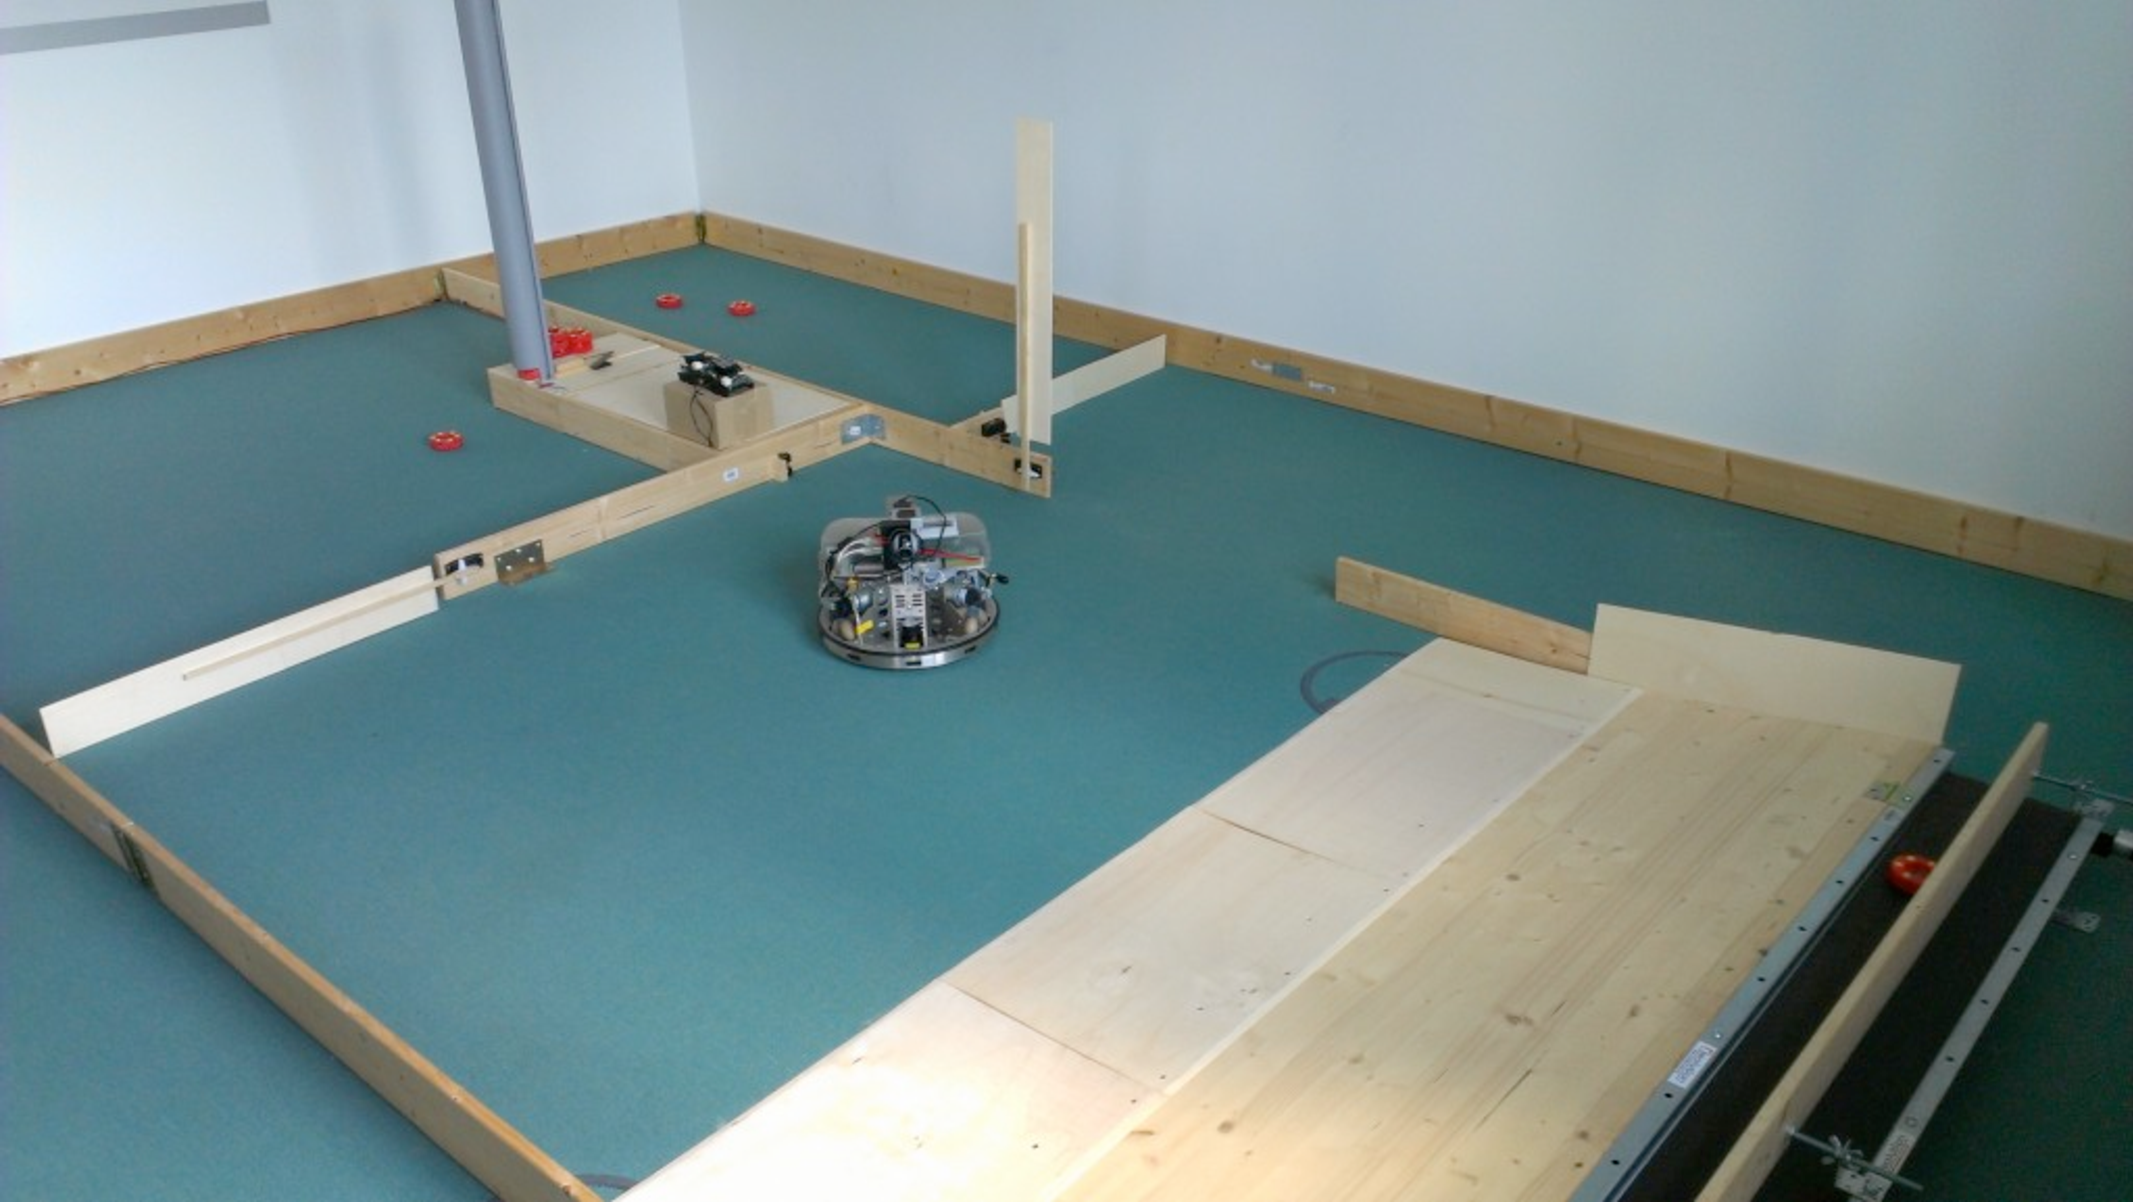
\includegraphics[width=0.8\textwidth]{figures/evaluation_scenario_2.pdf}
\caption{Photo of the lab (see \cite{Waetzoldt:2012pa})}
\label{fig:evaluation_scenario_2}
\end{figure}


We consider a robot system as depicted in Figure~\ref{fig:evaluation_scenario_2}, where a single robot has the duty to transport pucks as advised by the overall factory automation. The regular behavior of the robot is to move around, transport pucks, or charge its batteries. The behavior must meet strict constraints, such as preventing complete discharge of the batteries and with a lower priority, ensure to transport pucks as requested. It must also perform reasonably well with respect to some soft goals to minimize energy consumption and maximize throughput.

\begin{figure}[!htb]
\centering
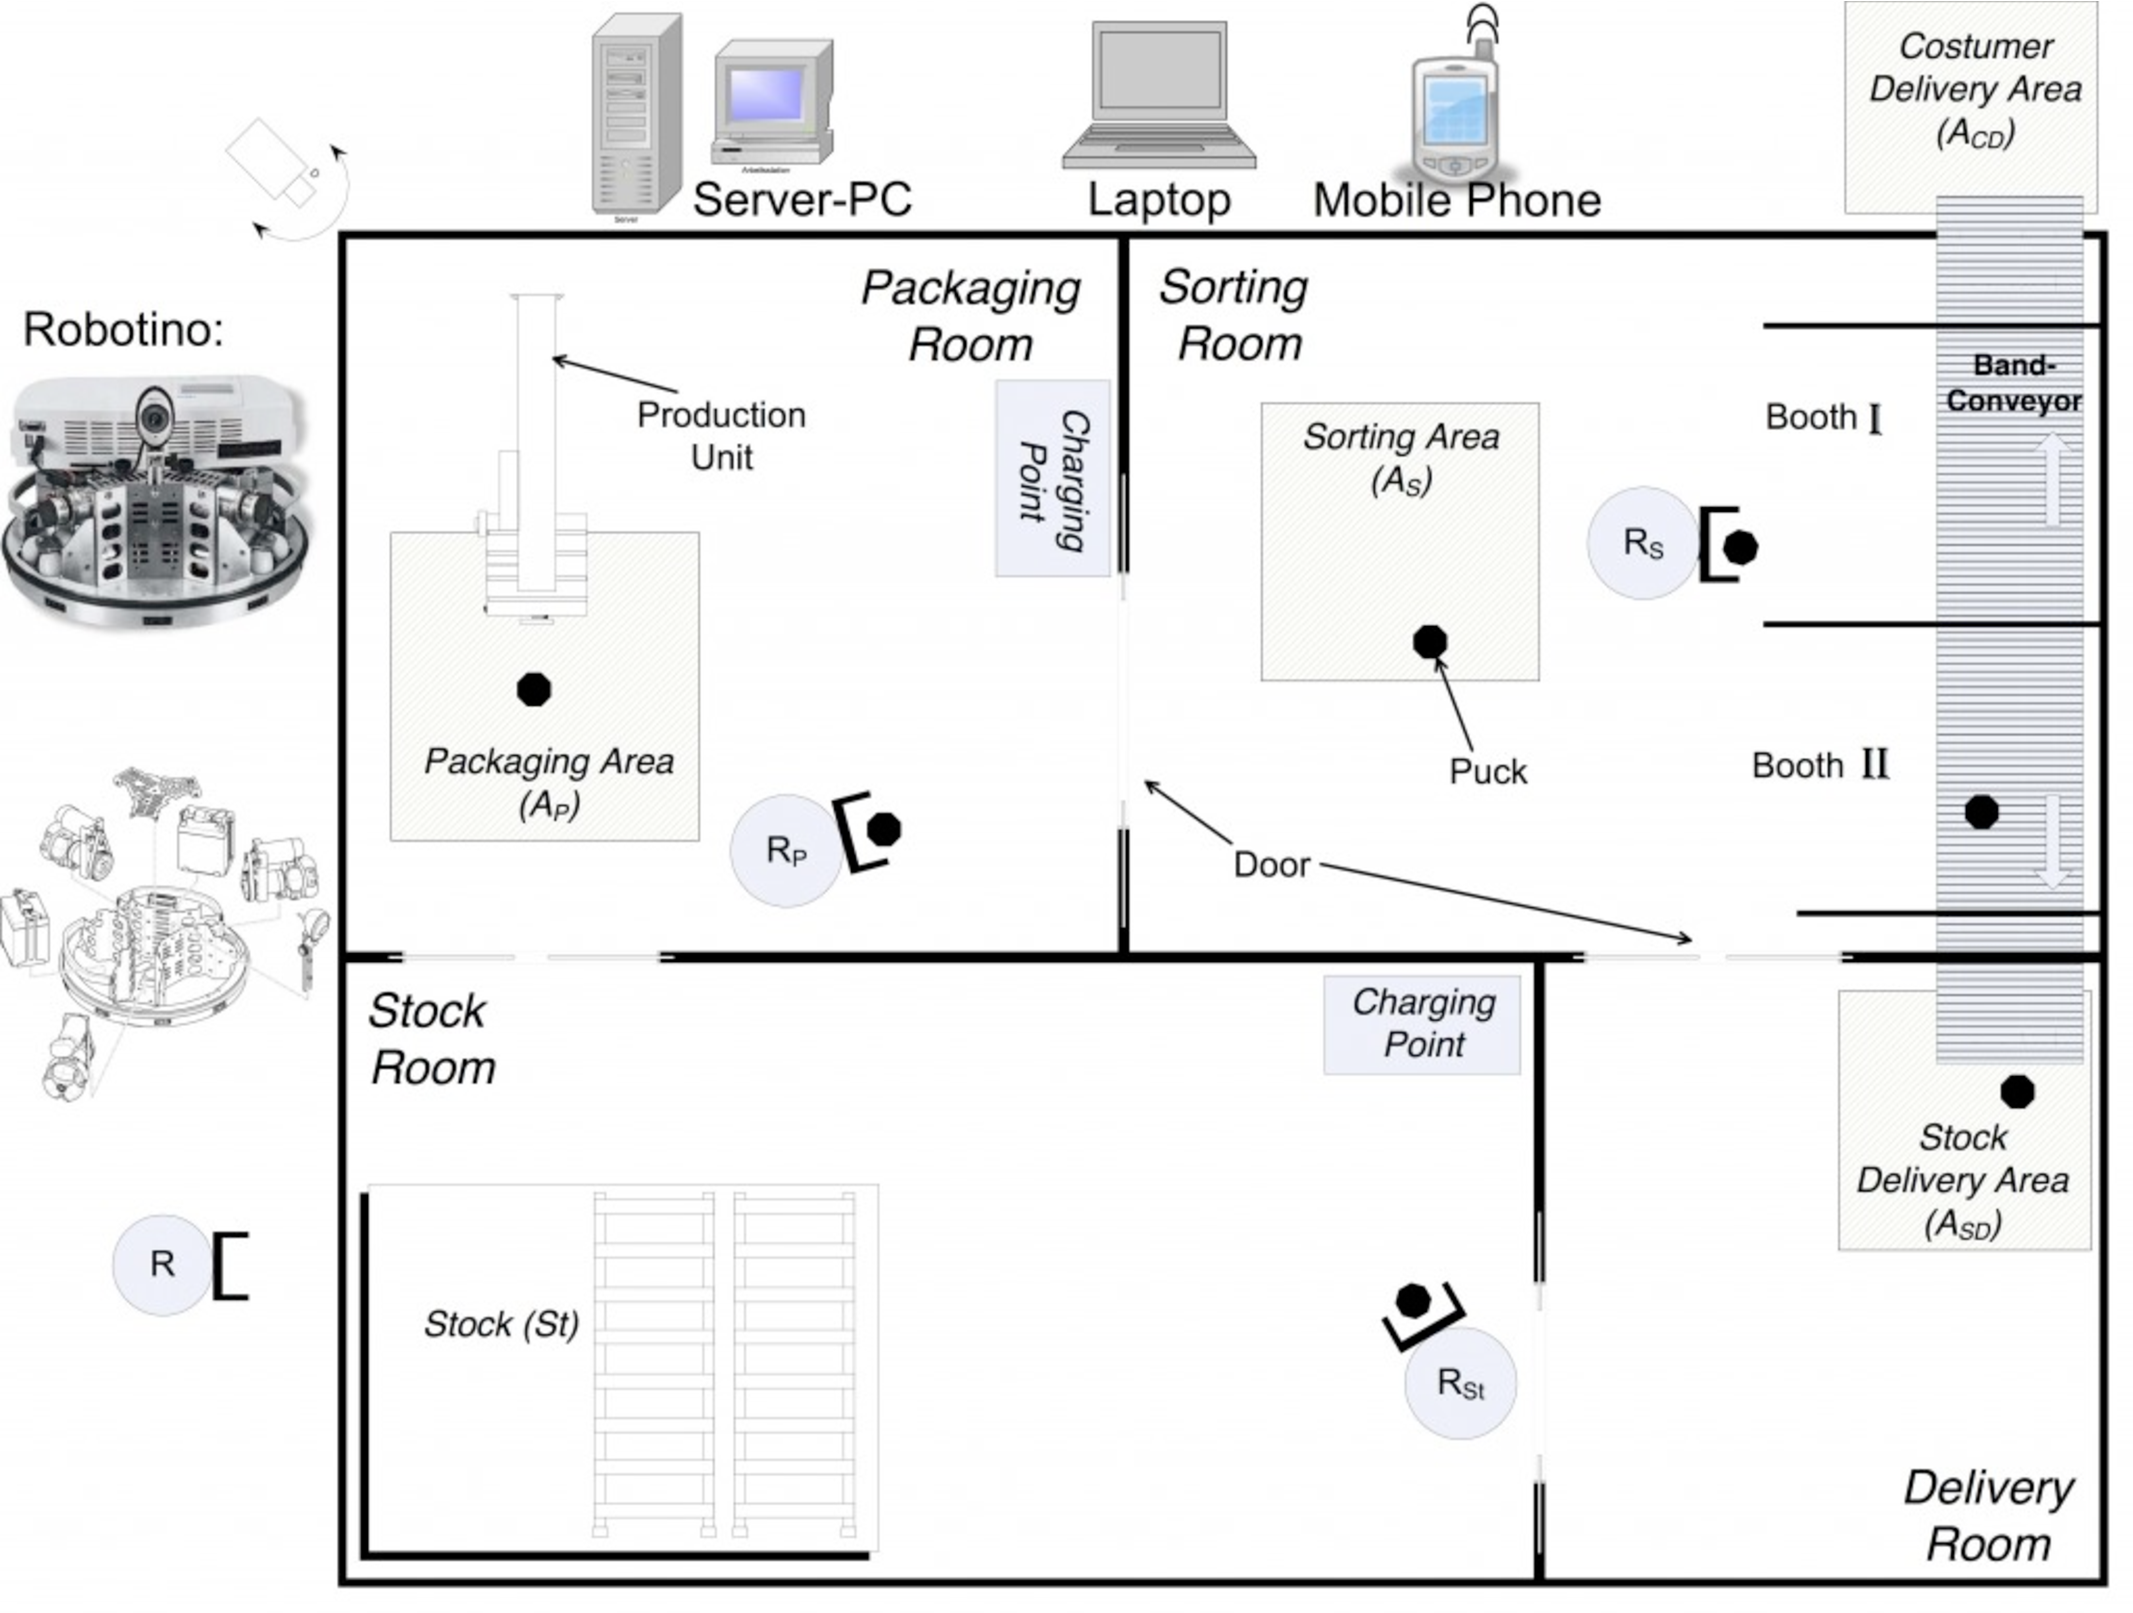
\includegraphics[width=0.8\textwidth]{figures/evaluation_scenario_1.pdf}
\caption{Structural\uidx{StructureCharacteristic} overview of the employed evaluation scenario (see \cite{Waetzoldt:2012pa})}
\label{fig:evaluation_scenario_1}
\end{figure}

Figure~\ref{fig:evaluation_scenario_1} depicts a structural\uidx{StructureCharacteristic} overview of the robot system. The whole cyber-physical evaluation scenario consists of four different rooms. In the first room, the pucks are packed and dropped for transportation in area $A_P$. A robot $R_P$ transports the puck to a second room and drops it within the sorting area $A_S$. Based on the current delivery status, the robot $R_S$ chooses one of the two booths and a band-conveyor transports the puck to the customer or stock delivery area ($A_{CD}$, $A_{SD}$) afterwards. In a third step, the robot $R_{St}$ transfers the puck to stock in $St$. The doors can be opened or closed dynamically to vary the scenario. A robot can charge its battery at one of the two charging points. Each robot acts as an autonomous unit. Therefore, the tasks transportation, sorting and stocking are independent from each other.

\begin{figure}[!htb]
\centering
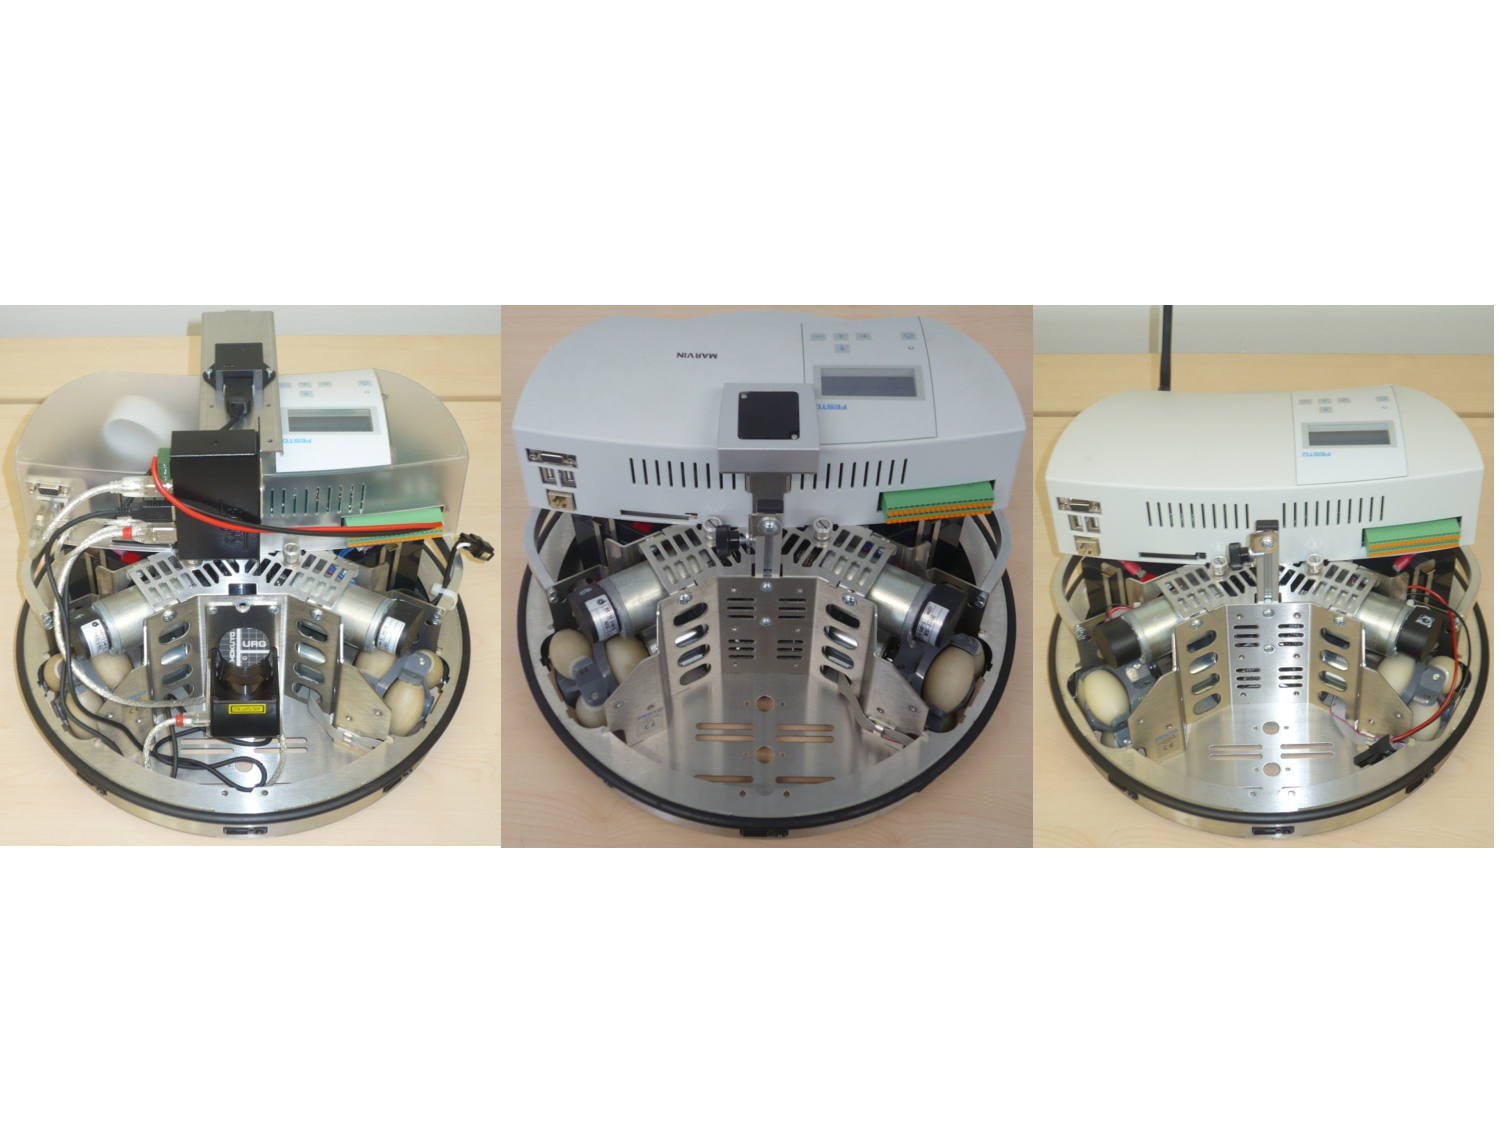
\includegraphics[width=0.8\textwidth]{figures/evaluation_scenario_3.pdf}
\caption{Photo of the employed robots (see \cite{Waetzoldt:2012pa})}
\label{fig:evaluation_scenario_3}
\end{figure}


For the evaluation of our research activities, we use our CPSLab robot laboratory consisting of three Robotino robots (see Figure~\ref{fig:evaluation_scenario_3}). The robots can be equipped with several sensors (e.g., laser scanner, infrared (IR) distance sensors, GPS-like indoor navigation systems) as well as different actuators (e.g., servo motors, omnidirectional drive, gripper). 

The general idea of our evaluation scenario is the realization of a variable production setting, where robots can transport small pucks (representing goods in a production system) to different locations. The robots must fulfill different requirements, e.g., they must provide basic functionality like moving and avoiding obstacles in hard real-time (reacting on obstacles within a few milliseconds). Further, the robots must achieve high level goals, e.g., energy saving of the battery, short routing to the destination points and optimizing the throughput while transporting the pucks. While basic functionalities, such as obstacle avoidance, must be realized in hard real-time, we use existing libraries to realize higher functionalities such as path planning or creating a map by evaluating measured distance values. The latter can rarely be realized under hard real-time constraints\uidx{Constraint} because of insufficient libraries. Furthermore, we run a RTAI Linux operating system on the robot to enable hard real-time execution.

% ========================================================================================
\subsection{CPS}\label{subsec:cpslab-cps}

In the following, we will use the details of the different development steps to outline how the development is linked to CPS and the concepts of the CPS ontology introduced in Chapter~\ref{ch:cps}.

% ============================================
\subsubsection{Simulation Stage}
%
The first step of the development process\uidx{Process} of Figure~\ref{fig:methodology} is a simulation stage that focus on the model development resp.~functional development for the employed control laws.
%
At this stage, many details resulting from the physical and cyber parts of the system are ignored resp.~simplified such as real sensor values with noise, specific effects of scheduling, the impact of communication interaction and messages, and timing/memory/computation constraints.

\begin{figure}[!htb]
\centering
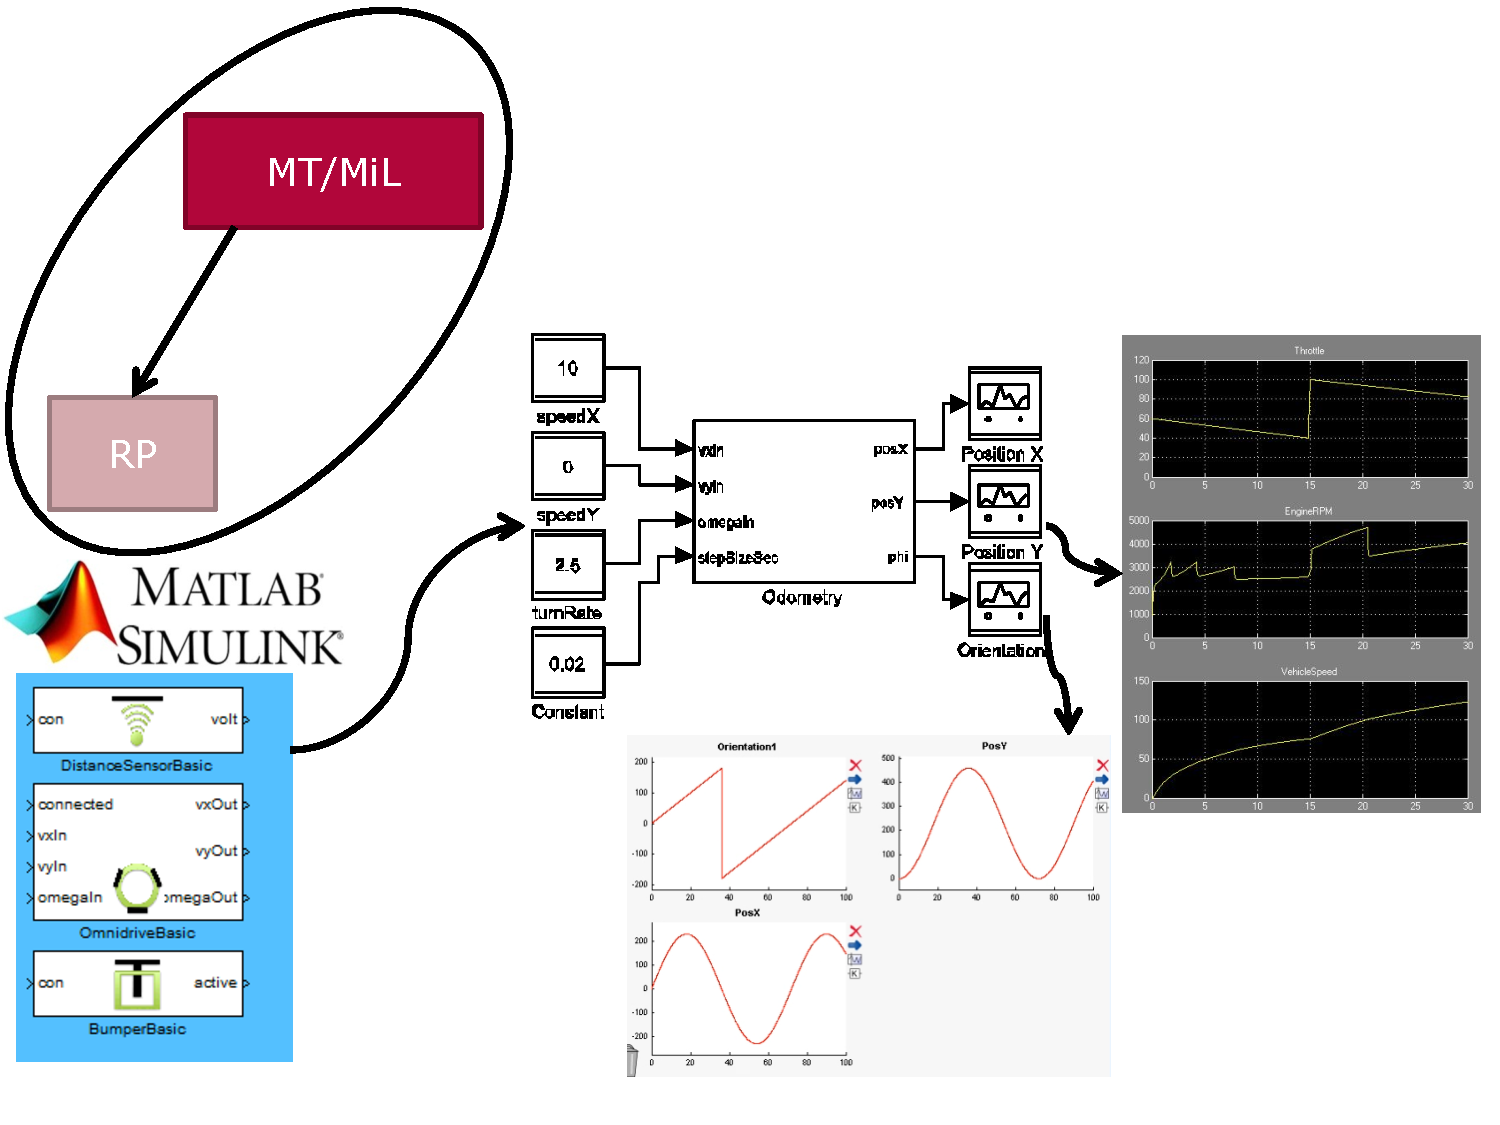
\includegraphics[scale=0.33]{figures/mt.pdf}
\caption{Overview of the model test in the simulation stage of \cite{Broekman&Notenboom2003}}
\label{fig:mt}
\end{figure}

% =========================================
\subsubsubsection{Model Test}
%
In a first activity\uidx{Activity} named \emph{model test} (MT)\uidx{ModelingActivity} (see Figure~\ref{fig:mt}), a so-called one-way/one-shot simulation with MATLAB/Simulink is supported where the model of the control behavior can be stimulated by inputs to see that they react properly. This provides some confidence that the setup control behavior works as intended.

% =========================================
\subsubsubsection{Model Test - CPS Ontology}
%
In the model test as outlined in Figure~\ref{fig:mt}, the abstract control algorithm from the cyber domain for a specific function is confronted with the physics as present in the input data plus expected outcomes relevant for the function and thus we have a very simple cyber-physical setting. 
%
Thus we cover the elements \CPSCyberPart from the CPS ontology for a particular function.


\begin{figure}[!htb]
\centering
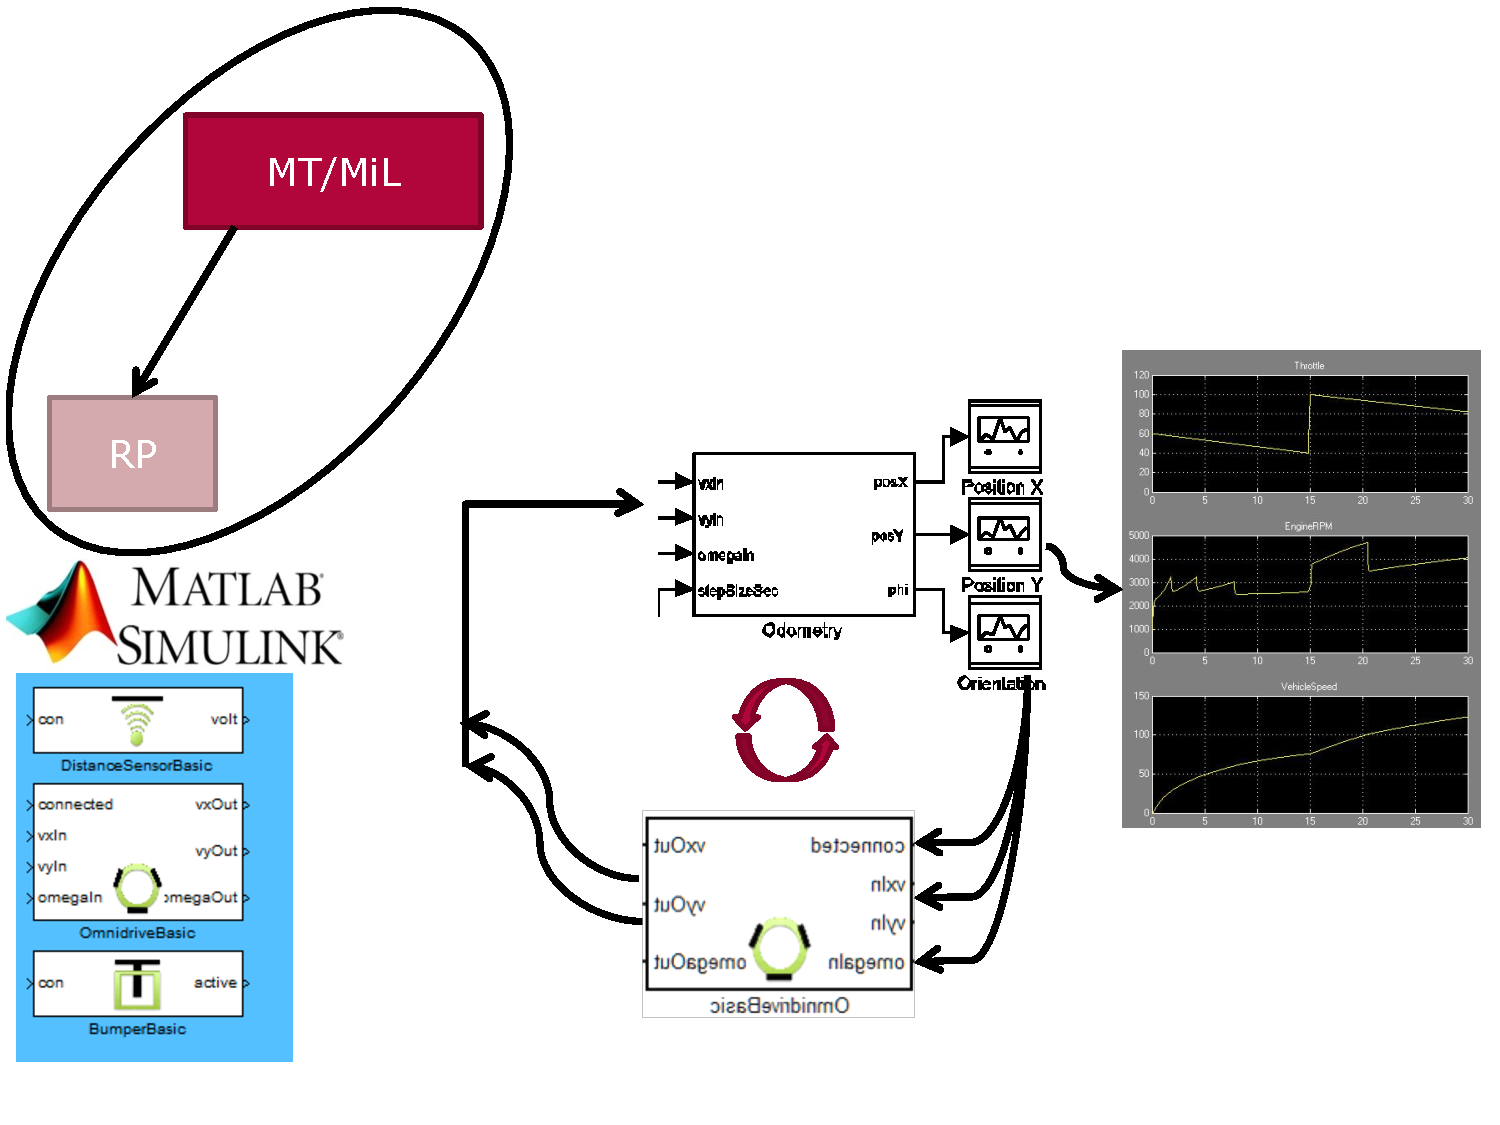
\includegraphics[scale=0.33]{figures/mil.pdf}
\caption{Overview of the model in loop simulation in the simulation stage of \cite{Broekman&Notenboom2003}}
\label{fig:mil}
\end{figure}


% =========================================
\subsubsubsection{Model-in-the-Loop}
%
In a second step, the model of the control behavior is combined with a MATLAB/Simulink model of the plant by means of a \emph{model-in-the-loop} (MiL) simulation as shown in Figure~\ref{fig:mil}, which uses the feedback provided by the plant model to evaluate that the control behavior is as expected. 

% =========================================
\subsubsubsection{Model-in-the-Loop - CPS Ontology}
%
The model in the loop depicted in Figure~\ref{fig:mil} in contrast, the abstract control algorithm from the cyber domain is combined with the idealized physics as present in the plant model and thus we have a simple cyber-physical setting. 
%
Here we cover thus the elements \CPSCyberPart and \CPSPhysicalPart from the CPS ontology for a particular function.



\begin{figure}[!htb]
\centering
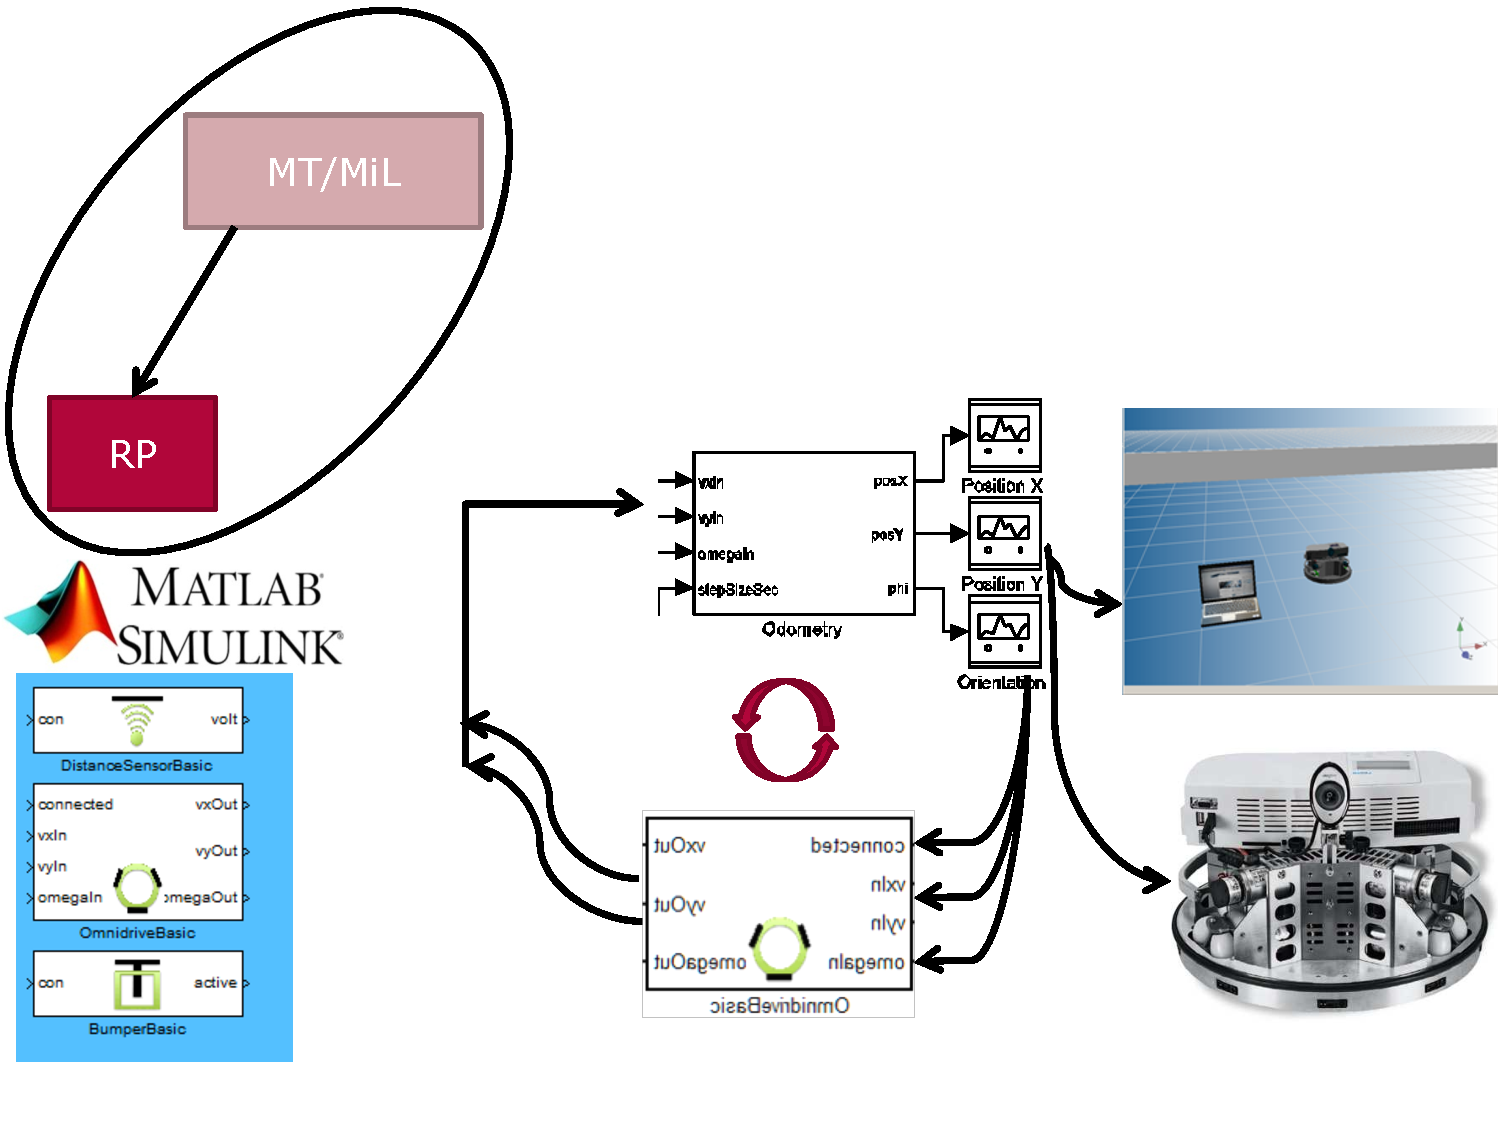
\includegraphics[scale=0.33]{figures/rp.pdf}
\caption{Overview of the rapid prototyping in the simulation stage of \cite{Broekman&Notenboom2003}}
\label{fig:rp}
\end{figure}



% =========================================
\subsubsubsection{Rapid Prototyping}
%
As the validity of plant models is often only rather limited when it comes to sophisticated aspects of the physical behavior\uidx{BehaviouralCharacteristic}, as an additional step \emph{rapid prototyping} as depicted in  Figure~\ref{fig:rp} is supported. 
%
For smaller control behavior, the model of the control behavior is linked to the real robot such that real sensor values with noise and timing constraints\uidx{Constraint} of the environment and platform can be covered. However, specific effects of scheduling, the impact of communication interaction and messages, and memory/computation constraints remain uncovered.
%
For larger scenarios and for the multi robot scenarios a link to a real hardware setup is not feasible here. Instead we employ a model-in-the-loop (MiL) simulation where a complex environment and the communication\uidx{Communication} between the robots can be explored. While this covers the impact of communication interaction and messages, other aspects like real sensor values with noise, specific effects of scheduling and timing/memory/computation constraints are, however, not covered.

% =========================================
\subsubsubsection{Rapid Prototyping - CPS Ontology}
%
The rapid prototyping against the robot as depicted in Figure~\ref{fig:rp}, the abstract control algorithm from the cyber domain is brought together with the real physics of the robot  and thus we have clearly a cyber-physical setting. 

Our rapid prototyping being based on a sophisticated robot simulator, again the abstract control algorithm from the cyber domain is brought together with the physics as present in the sophisticated robot model of the simulator and thus we have clearly a cyber-physical setting. 

In both cases we thus cover the elements \CPSCyberPart from the CPS ontology for a particular function and the elements \CPSPhysicalPart from the CPS ontology for the part of the robot relevant for a particular function that is either simulated or considered directly.






% ============================================
\subsubsection{Prototyping Stage}
%
The second supported stage is the prototyping stage where the focus changes from models to their implementation in software or hardware and where besides the individual functions also the system architecture is covered. Due to this refined view, in particular discretization effects of the cyber part\uidx{SystemPart} that are absent in the abstract mathematical models employed in the former stage now become visible.
%
At this stage, less details are ignore resp.~simplified as step by step specific effects of scheduling, the impact of communication\uidx{Communication} interaction and messages, and timing/memory/computation constraints\uidx{Constraint} are taken into account.


\subsubsubsection{More Detailed Modeling}
%
To consider the more detailed view\uidx{View} outlined, at the prototyping stage the models must be refined such that besides the individual functions also the system architecture is defined.

\begin{figure}[!htb]
\centering
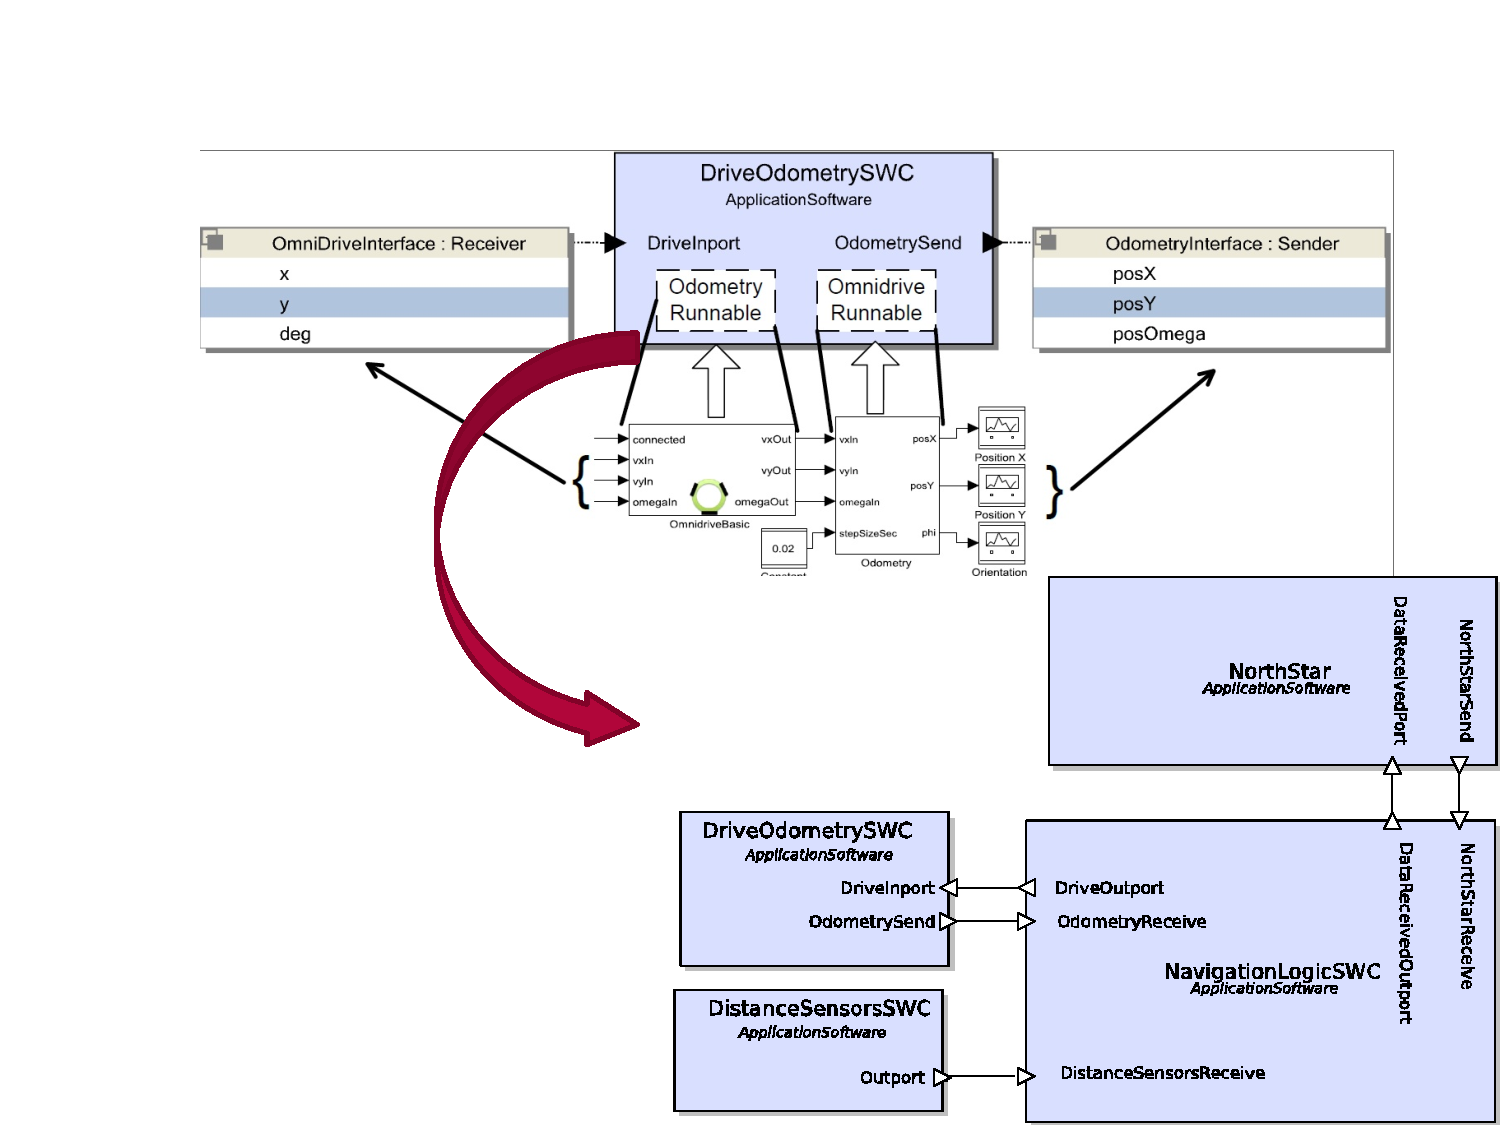
\includegraphics[scale=0.33]{figures/arch.pdf}
\caption{Overview of the definition of the software architecture in the prototyping stage of \cite{Broekman&Notenboom2003}}
\label{fig:arch}
\end{figure}

As depicted in Figure~\ref{fig:arch}, this is done by first defining components\uidx{Component} and their communication\uidx{Communication} via port types, messages, interfaces, and data types with AUTOSAR and map the beforehand considered functional parts on them. In this step, we also have to map the functionality extending the existing models and where necessary add custom implementation files.
%
In a second step, we then define the overall architecture using AUTOSAR including besides the components and their communication also task specification and the hardware configuration.


\begin{figure}[!htb]
\centering
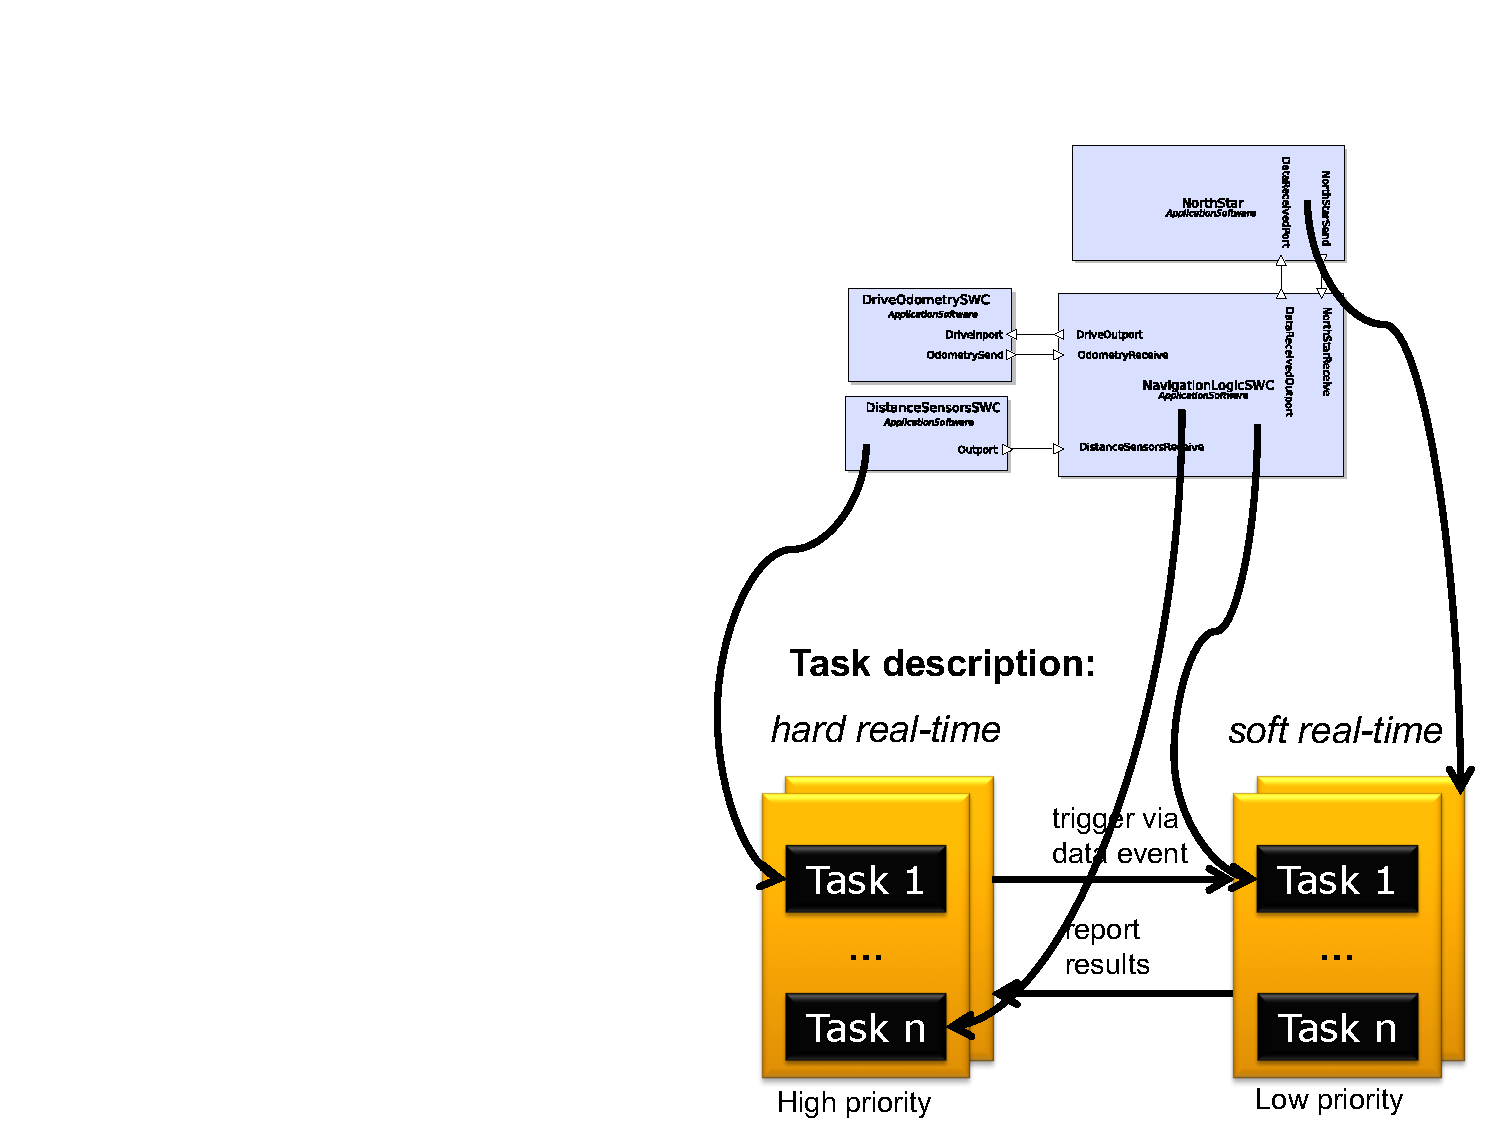
\includegraphics[scale=0.33]{figures/map.pdf}
\caption{Overview of the mapping of the architecture to tasks and communication\uidx{Communication} in the prototyping stage of \cite{Broekman&Notenboom2003}}
\label{fig:map}
\end{figure}

As depicted in Figure~\ref{fig:map}, an important element of this refinement is also real-time constraints, e.g. to guarantee safety\uidx{Safety} constraints\uidx{Constraint}. A combination of hard and soft real-time aspects at functional as well as architectural levels must be defined including a mapping to hard and soft real-time task with proper levels for the priorities.
%Where necessary such a refinement has to preserves hard real-time constraints for basic functions and the communication has to be designed such that it also is not in conflict with any hard real-time constraints and that the interaction between hard and soft real-time behavior ensures consistent and timely data exchange.


%\subsubsubsection{Verification}
%\subsubsubsection{SiL}
%
Concerning the verification, we employ code generation at the prototyping stage and try to step by step add more and more details of the software and hardware to the picture in the following steps.

\begin{figure}[!htb]
\centering
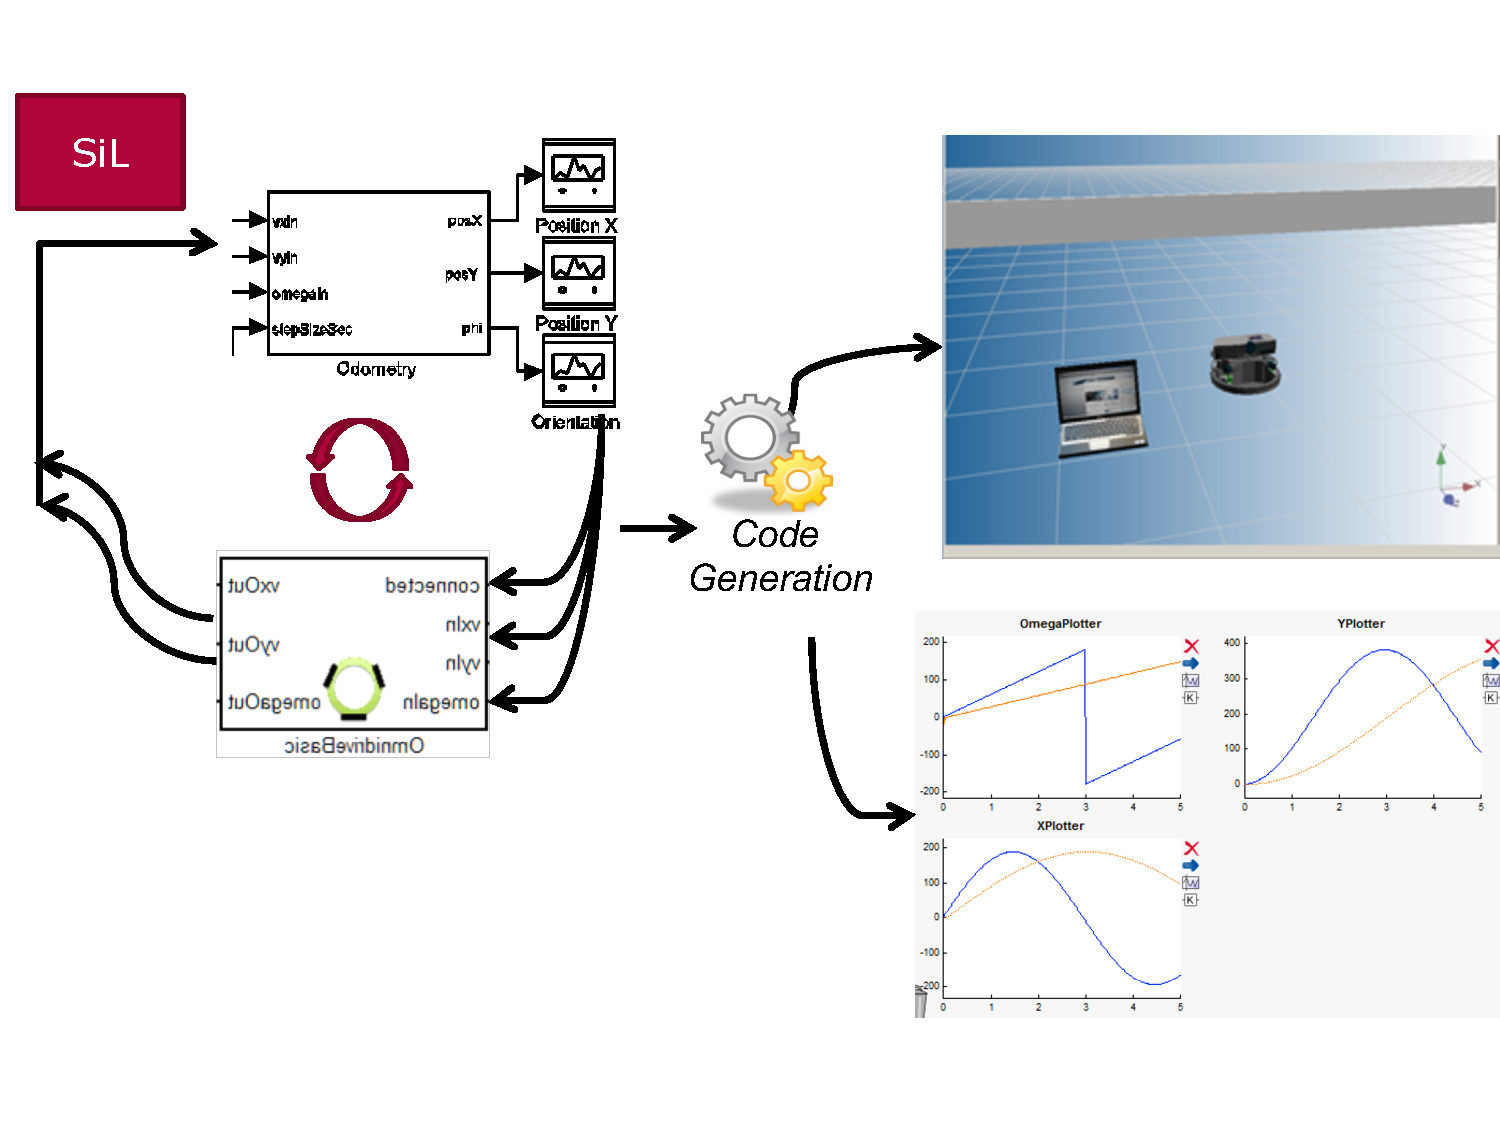
\includegraphics[scale=0.33]{figures/sil.pdf}
\caption{Overview of software-in-the-loop (sil) simulation in the prototyping stage of \cite{Broekman&Notenboom2003}}
\label{fig:sil}
\end{figure}



% ============================================
\subsubsubsection{Software in the Loop (SiL)}
%
The \emph{software-in-the-loop} (SiL) simulation at the prototyping stage as depicted in Figure~\ref{fig:sil} requires that code generation is employed to derive code for the functional models and architectural models. In special cases, also additional manually developed code has to be integrated. Then, the code is executed and run against the available simulation of the robot and its environment.

As we are still not using the real hardware, we still ignore and simplify elements such as real sensor values with noise %and not by the simulator covered timing constraints\uidx{Constraint} 
of the environment or platform, specific effects of scheduling, and timing/memory/computation constraints of the software.

% ============================================
\subsubsubsection{Software in the Loop (SiL) - CPS Ontology}
%
The first form of software in the loop (SiL) for which the software is executed on a desktop computer against a robot simulator features that the detailed control algorithm from the cyber domain is brought together with the physics as present in the sophisticated robot model of the simulator. Therefore, we clearly have a cyber-physical setting. 

The second form of SiL for which the software is also executed on a desktop computer but against a remotely controlled robot makes that the detailed control algorithm from the cyber domain is brought together with the physics as present in the remotely controlled robot. Therefore, we clearly have a cyber-physical setting. 

In both cases we cover the elements \CPSCyberPart from the CPS ontology for the combination of all function and the elements \CPSPhysicalPart from the CPS ontology for the whole robot.

%\subsubsubsection{HiL}

\begin{figure}[!htb]
\centering
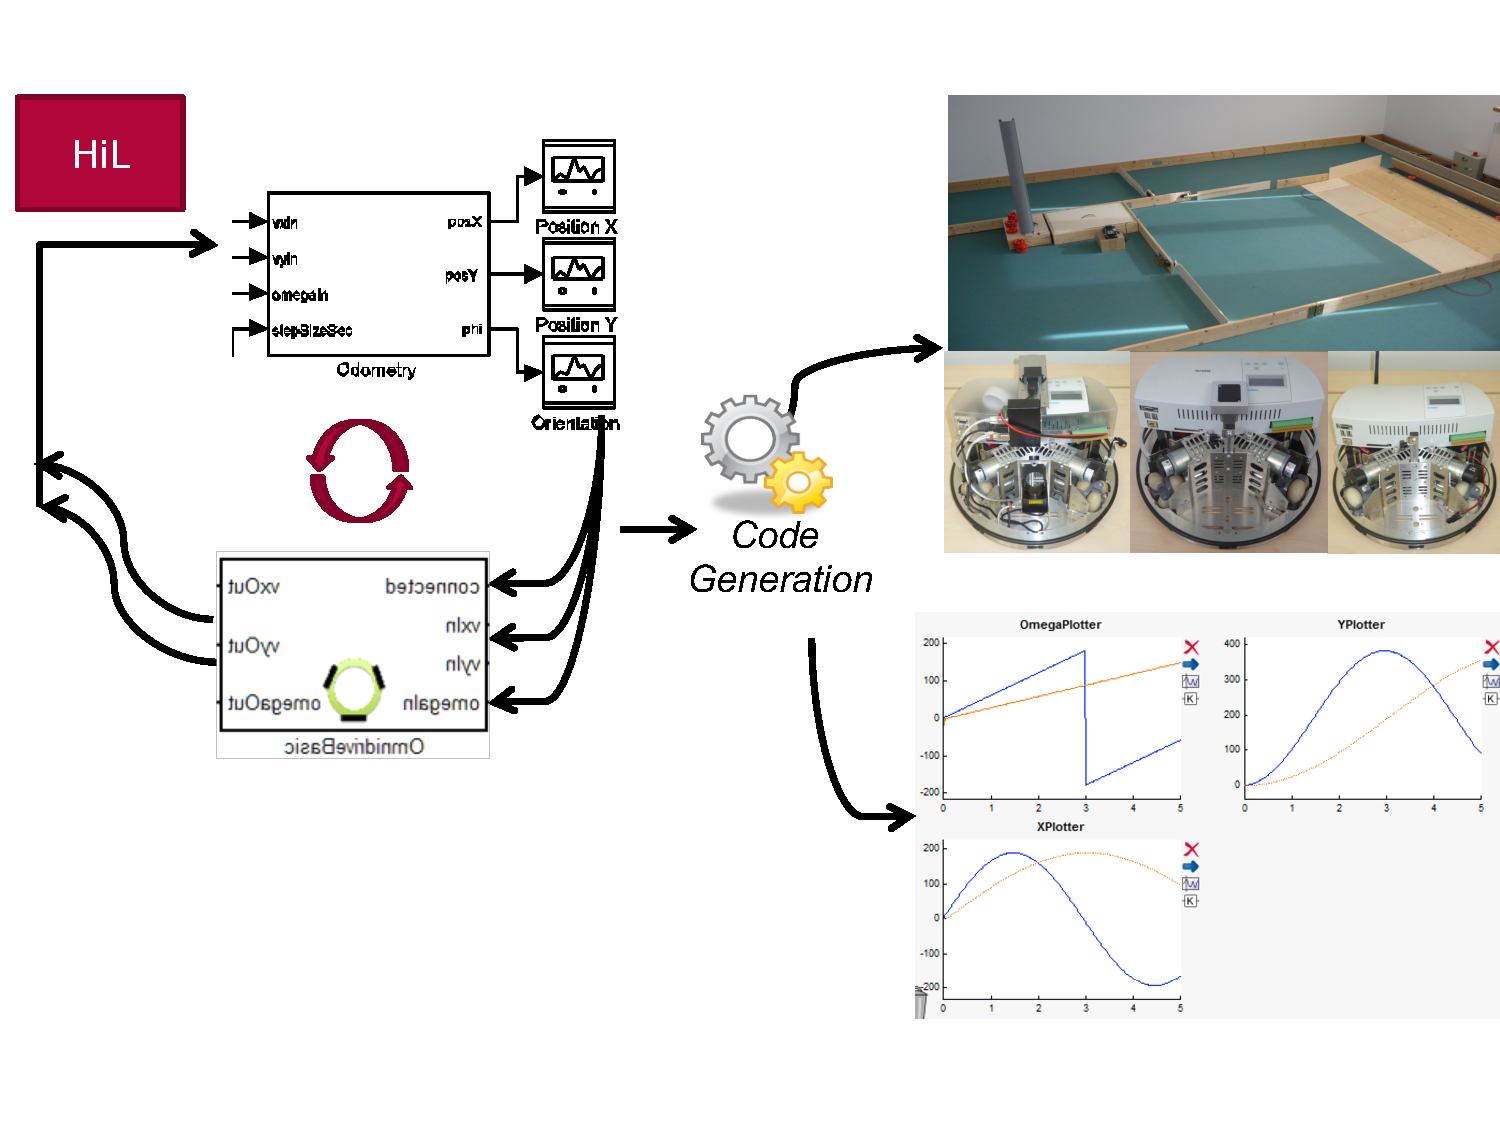
\includegraphics[scale=0.33]{figures/hil.pdf}
\caption{Overview of hardware-in-the-loop (HiL) testing in the prototyping stage of \cite{Broekman&Notenboom2003}}
\label{fig:hil}
\end{figure}


% ============================================
\subsubsubsection{Hardware in the Loop (HiL)}
%
By moving on to the lab itself, we can then also consider a \emph{hardware-in-the-loop} (HiL) simulation at the prototyping stage as sketched in Figure~\ref{fig:hil}. Besides the software that is generated or integrated, the specific characteristics of the robot hardware and lab environment and its hardware can also be experienced.

As we now employ the real hardware, we no longer ignore resp.~simplify any elements. Therefore, now real sensor values with noise, specific effects of scheduling, the impact of communication interaction and messages, and timing/memory/computation constraints\uidx{Constraint} are all considered.

% ============================================
\subsubsubsection{Hardware in the Loop (HiL) - CPS Ontology}
%
The hardware in the loop (HiL) executing the software on the robot depicted in Figure~\ref{fig:hil} ensures that the detailed control algorithm from the cyber domain is brought together with the physics as present in the robot and thus we have clearly a cyber-physical setting. 

Thus we cover the elements \CPSCyberPart from the CPS ontology for the combination of all function and the elements \CPSPhysicalPart from the CPS ontology for the whole robot.




% ============================================
\subsubsection{Pre-Production Stage}
%
In our specific setting and due to our focus on the software development, the \emph{system test} in the pre-production stage is not really different as we do not produce any system we want to sell later. In a commercial setting the robots in the prototyping, the robots in the lab would likely be equipped with more testing hardware or prototypical hardware, while in our lab only one level exists here.

The outlined methodology and tool chain adjusted from the automotive domain, provides suitable guidance due to the different focus in stages and follows where possible an MDE approach where tools and libraries are integrated such that the models drive the development. Only later the code and configuration data automatically generated from the models are employed to consider more details concerning the verification, simulation, and testing.
%
We put special focus on supporting also hard and soft real-time considerations, which are oftentimes ignored in robotic development scenarios.

%\TODONOTE{ HG: add steps when considering multiple robots? }



%\LATER{ HG: The links to the CPS ontology that are present in the case study are quite weak and so far only refer to the elements. Maybe we can refine them when the improved version of the CPS ontology is available? 
%Right now we have:
%- separation into physical and cyber elements covered by the ontology are referenced
%- maybe properties of the CPS can be added?
%}





% ========================================================================================
\subsection{MPM}\label{subsec:cpslab-mpm}

For the MPM ontology introduced in Chapter~\ref{ch:mpm}, we will in the following use the details of the different development steps to outline how the development is linked to MPM.

% ============================================
\subsubsection{Overview}
%


\SKIP{
\begin{figure}[!htb]
\centering
\includegraphics[width=0.8\textwidth]{figures/toolchain.pdf}
\caption{Overview of the employed tool chain (see \cite{Waetzoldt:2012pa})}
\label{fig:toolchain}
\end{figure}

An additional element depicted in Figure~\ref{fig:toolchain} is a prototype tool we developed to map AUTOSAR models to a real-time simulator from INCRON to permit detailed performance evaluation early on in parallel to SiL activities.
%
Another extension not depicted in Figure~\ref{fig:toolchain} is a link between the SysML tool TOPCASED and the dSPACE tool SystemDesk for AUTOSAR that permits to derive the software and hardware architecture in AUTOSAR from the SysML system engineering models.
%
However, to keep things simpler we omit both extensions in our detailed description and the sketches of the megamodels.

\begin{figure}[!htb]
\centering
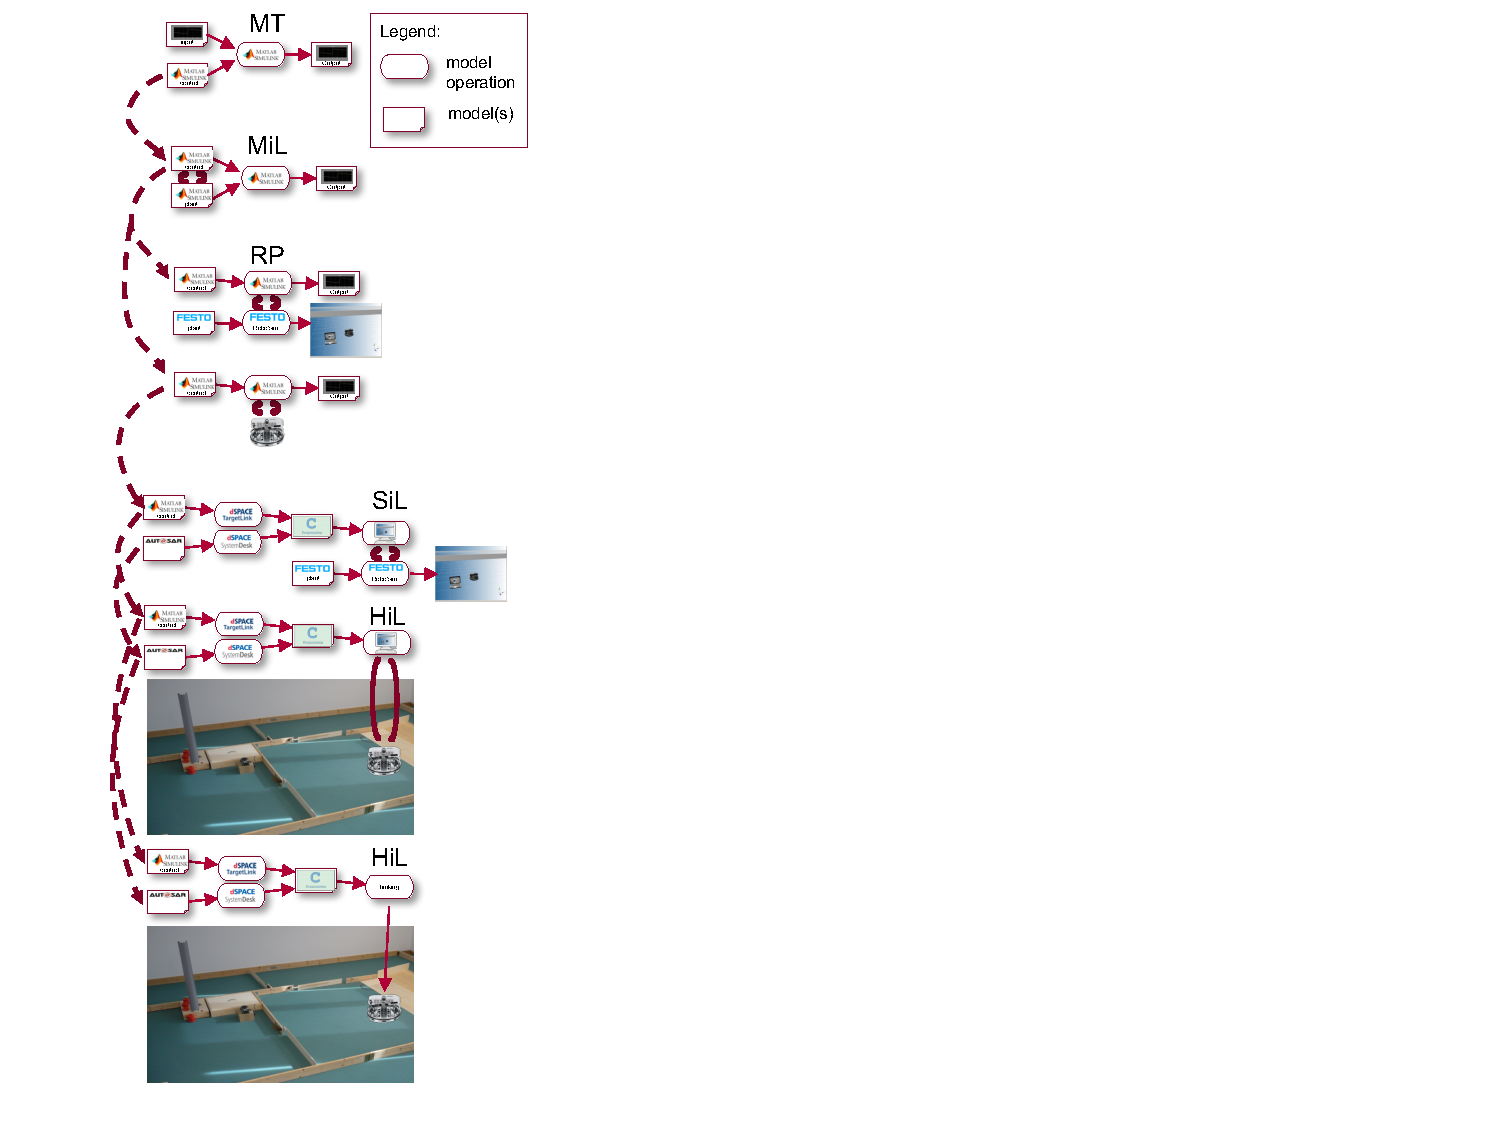
\includegraphics[scale=1.25]{figures/mm.pdf}
\caption{Sketch of the megamodel of the different stages of \cite{Broekman&Notenboom2003}}
\label{fig:mm}
\end{figure}

While several tools are employed at several stages and activities, the models developed for each of these activities are quite different as visible in the megamodel depicted in Figure~\ref{fig:mm}.

}

\begin{figure}[!htb]
\centering
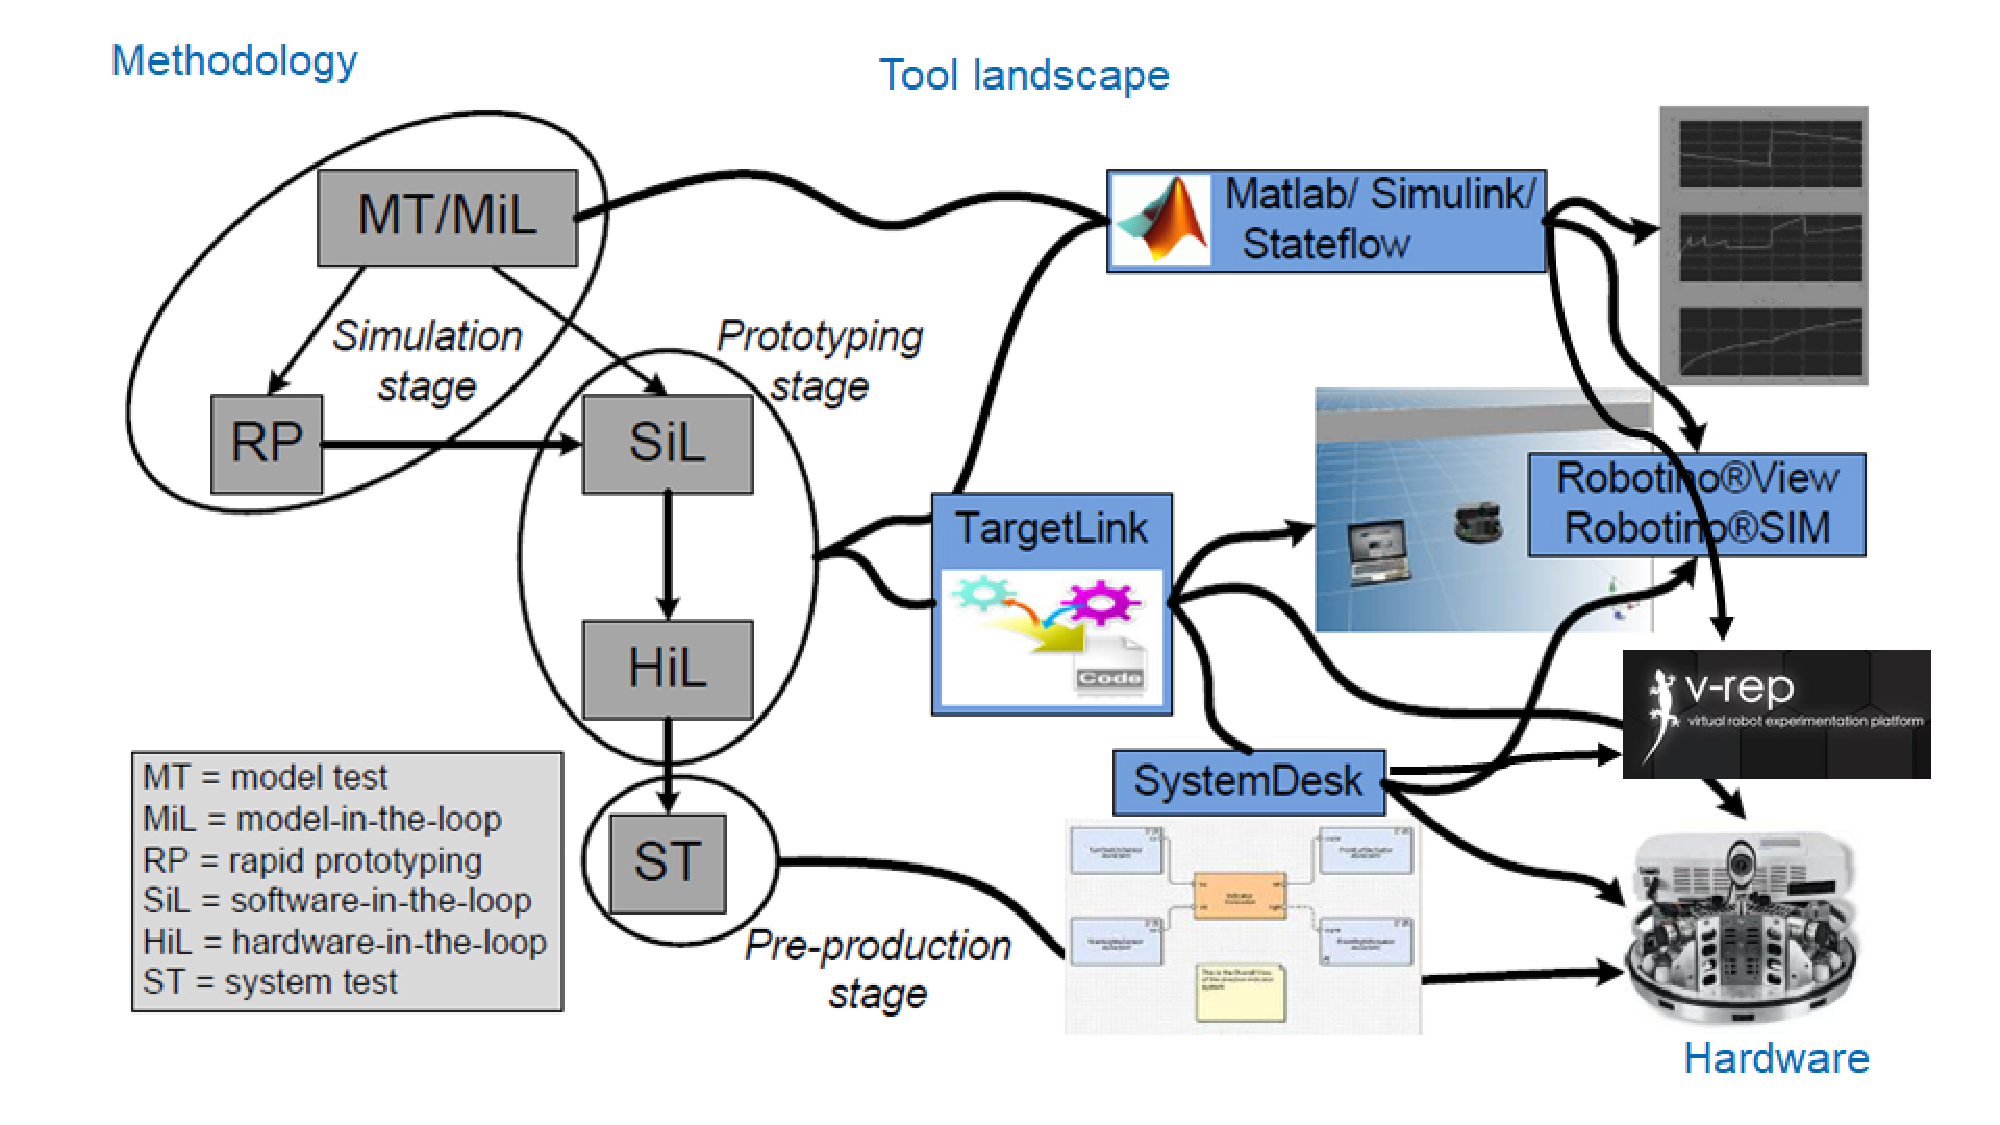
\includegraphics[width=0.9\textwidth]{figures/mm-hpi2.pdf}
\caption{Tool landscape and its relation to the development methdology}
\label{fig:MMFig2}
\end{figure}

%\todo{DB: Should that be part of the MPM section? HG: yes}
In Figure~\ref{fig:MMFig2} the tool landscape for developing the aforementioned robot CPS is depicted. It consists of
%
MATLAB/Simulink for modeling and simulation,
%
dSPACE SystemDesk for modeling software architecture, hardware configuration, and task mapping,
%
dSPACE TargetLink for code generation and
%
the FESTO Robotino-Library with the FESTO Robotino{\copyright}Sim simulator.

\begin{figure}[!htb]
\centering
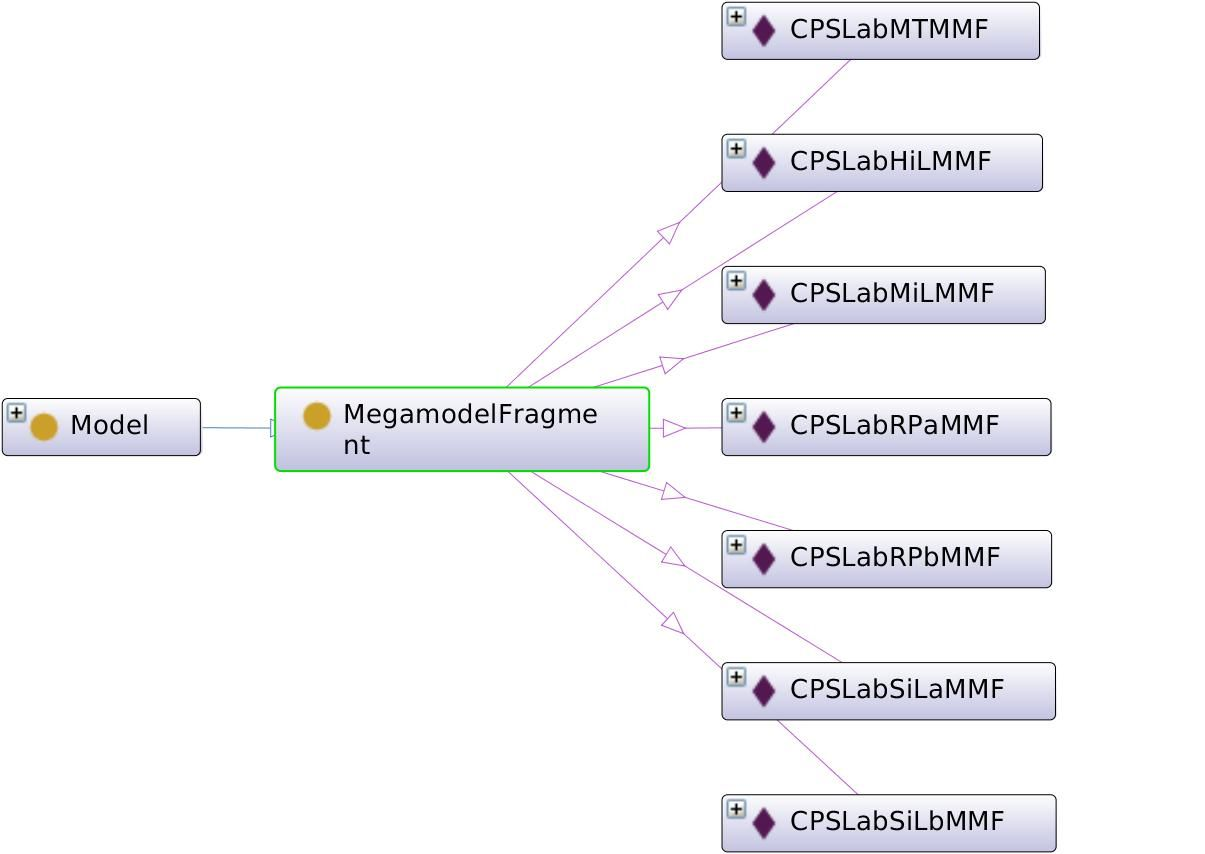
\includegraphics[scale=0.4]{figures/CPSLabMTMMF-NEW.jpeg}
\caption{All megamodel fragments\uidx{MegamodelFragment} of the \CPSLabMM megamodel\uidx{Megamodel}}
\label{fig:MegaModelFragmentsForCPSLabMM}
\end{figure}
 
%\begin{figure}[!htb]
\begin{figure}[p]
\centering
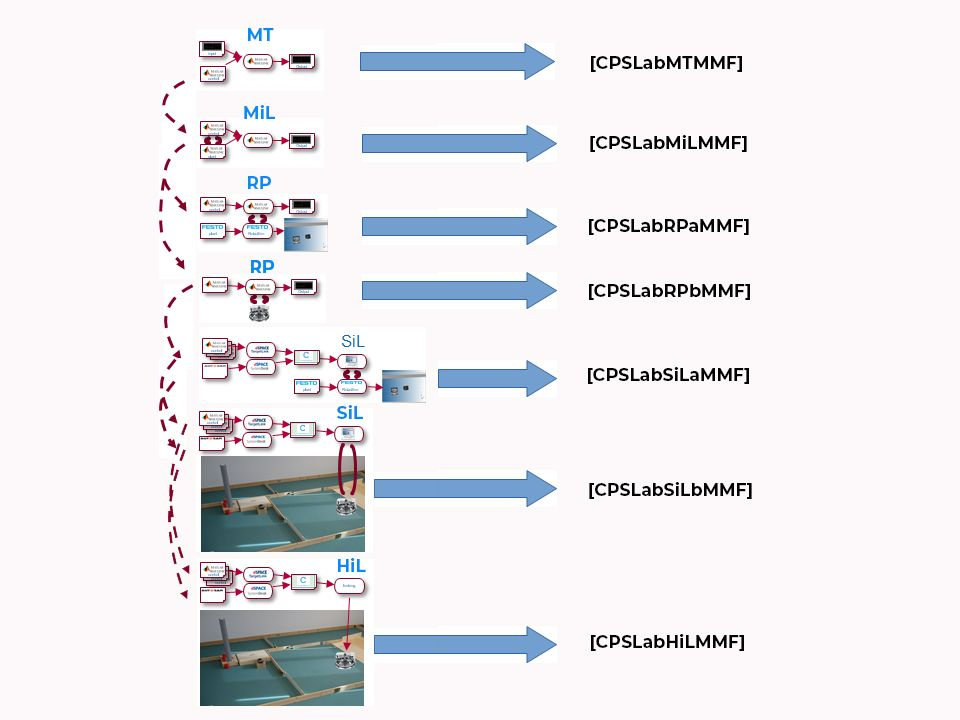
\includegraphics[scale=0.6]{figures/slide-fig.jpg}
\caption{Overview over the megamodel fragments of the CPSLab megamodel\uidx{Megamodel} and how the models are related (dashed arrows)}
\label{fig:MMFig10}
\end{figure}

%\TODOINLINE[SB]{ HG: Please add names of the megamodelfragments to the graphics of Figure~\ref{fig:MMFig10}. We should use the names defined int the subsequent figures which show the fragments of the megamodel in our PPT-slide notation MT (see Figure \ref{fig:CPSLabMTMMF} for a case where MT (for Model Test) and  \CPSLabMTMMF (as the name of the related MegaModelFragmeent) should be added. In most case the short name (e.g., SiL) has been already added. }

%\TODOINLINE[SB]{ HG: Please remove the methodology part in Figure~\ref{fig:MMFig10} (large red boxes with MT, MiL, RP, ... as this has been shown on the former figure already. Please ove the legend to the the remaining graphicasl elements.}

On overview about the stages and activities with an emphasis on models, tools, and multi-paradigm modeling is depicted in Figure~\ref{fig:MMFig10}.

In the following, we outline to which elements of the MPM ontology of Chapter~\ref{ch:mpm} the elements of the megamodel\uidx{Megamodel} refer and which megamodel fragments\uidx{MegamodelFragment} cover the scenarios introduced in the last subsection.

%\LATER{ HG: Is an introduction to the notation required? Do we have to explain the links to the MPM ontology concepts here?}

\subsubsubsubsection{Formalism, Languages, Models, and Tools}

\LATER[Formalism]{
\item Formalism
    \begin{itemize}
        \item Automated Based Formalism: Abstract state machine, Cellular automata, Input/Output Automata, Label transitions systems, Timed transitions systems
        \item Automated Based Formalism:: Hybrid Automata: Hybrid Automata, Hybrid Input/Output automata, Linear hybrid automata, Non-Linear Hybrid Automata, Stocastics hybrid automata 
        \item Automated Based Formalism:: Hybrid Automata:: Timed Automata: , Stockists timed automata, Timed Automata, PTS.
        \item Flow Based Formalism: Data Flow, State Flow, Data Flow timed, HyFlow.
        \item Logic Based Formalism: First order logic, Linear temporal logic, CTL, Temporal Logic 
        \item Petri net based formalism: High Level Petri net, Petri net, Petri net with priyority, Petri net with time, dPN, Timed Petri net
        
    \end{itemize}
}

\begin{itemize}
    \item Used Language and Models
    \begin{itemize}
        \item \MATLABSimulinkLanguage: \CPSLabControlModel, \CPSLabPlantModel
        \item \FESTORobotinoSimLanguage: \CPSLabRobotModel
        \item \AUTOSARLanguage: \CPSLabSystemModel
    \end{itemize}
    \item MegaModel\uidx{Megamodel}
    \begin{itemize}
        \item MegaModel: \CPSLabMM
        \item MegaModelFragments\uidx{MegamodelFragment}: \CPSLabMTMMF, \CPSLabMiLMMF, \CPSLabRPaMMF, \CPSLabRPbMMF, \CPSLabSiLaMMF, \CPSLabSiLbMMF, \CPSLabHiLMMF
        \item ModelRealtions: (see detailed definition of the megamodel fragments)
    \end{itemize}
    \item Tool
    \begin{itemize}
        \item SimulationTool: \MATLABSimulinkSimulator
        \item TransformationTool: \dSPACETargetLink
        \item ModelingTool: \dSPACESystemDesk
        \item SimulationTool: \FESTORobotinoSim
        \item VisualizationTool: \FESTORobotinoView
        \item ExecutionTool: \DesktopExecution
        \item ExecutionTool: \RobotExecutionRemote
        \item ExecutionTool: \RobotExecutionLocal \LATER{ HG: check tool types!}
    \end{itemize}
\end{itemize}

%\DONE[HG]{ HG: please add scheme for MPM ontology use here! }
%\DONE[SB]{ HG: please model scheme for MPM ontology presented here with Protege! }
%\DONE[SB]{ HG: please add figure showing the used MPM ontology elements here! }



The added elements for the CPSLab ontology outlined in the text are depicted also in Figure~\ref{fig:MegaModelFragmentsForCPSLabMM}.

% ============================================
\subsubsection{Simulation Stage}
%
In the simulation stage we have two development activities: model test and model-in-the loop.
%
In the following, we will outline how they can be captured with mega-model fragments consisting of model instances and tool applications.





% =========================================
\subsubsubsection{Model Test}
%
The model test introduced in Figure~\ref{fig:mt}, is rather trivial as it only employ a single model of the planned control algorithm plus some auxiliary models for test inputs. Then, as depicted in Figure~\ref{fig:MMFig3} the model of the control algorithm is simulated by employing the test inputs.

\begin{figure}[!htb]
\centering
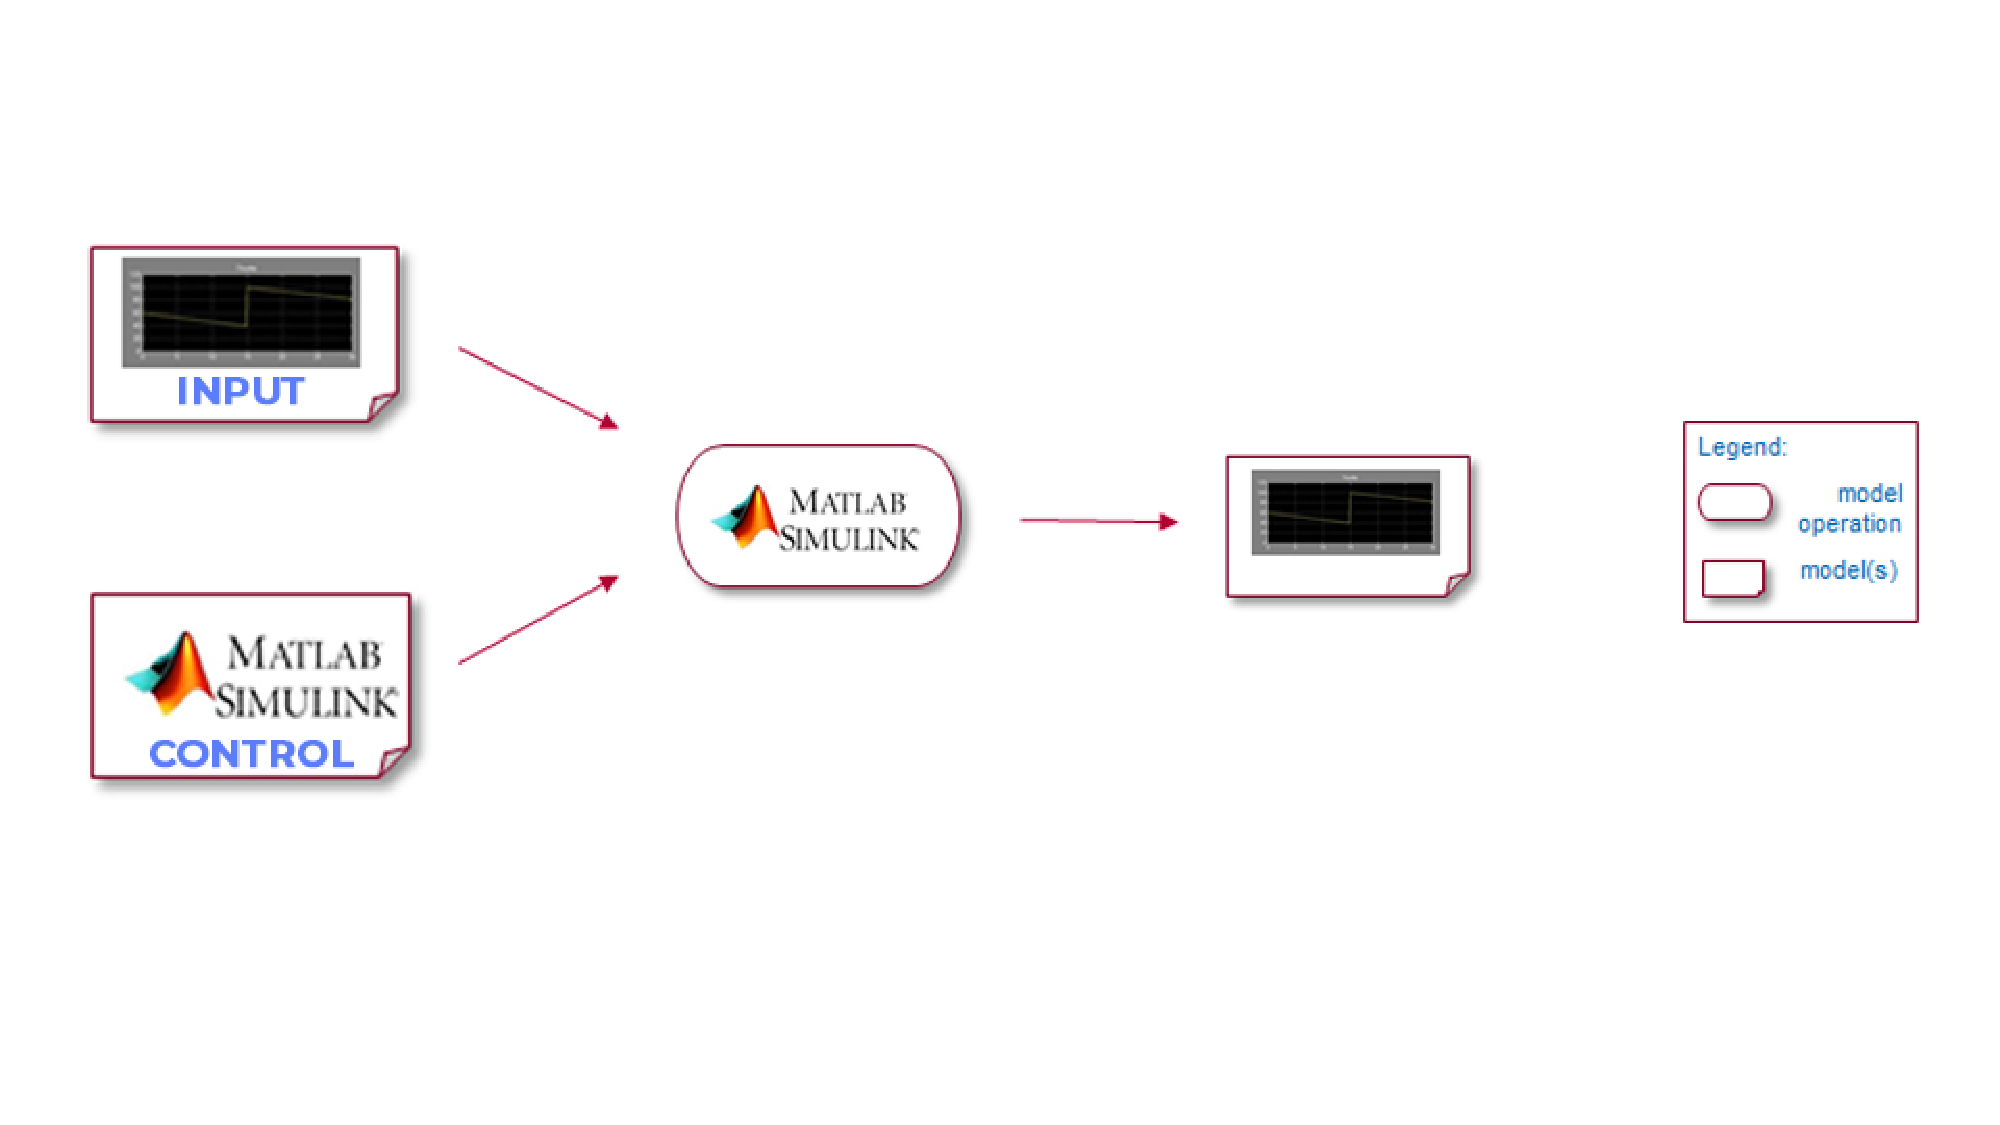
\includegraphics[scale=0.33]{figures/mm-hpi3.pdf}
\caption{Model Test}
\label{fig:MMFig3}
\vspace{-0.2in}
\end{figure}

% =========================================
\subsubsubsection{Model Test - MPM Ontology}
%
%
\subsubsubsubsection{MegaModel Fragment \CPSLabMTMMF}

\begin{itemize}
    \item MegaModelFragment: \CPSLabMTMMF
    \begin{itemize}
        \item Model(s): \CPSLabControlModel
    \end{itemize}
\end{itemize}

\subsubsubsubsection{Tools / Models Operations of \CPSLabMiLMMF}

\begin{itemize}
    \item \uidxp{ModelOperation}: One Shot Simulation
    \begin{itemize}
        \item Input Model(s): \CPSLabControlModel, Input data (entered with \MATLABSimulinkSimulator)
        \item Output Model(s): Output data (visualized with \MATLABSimulinkSimulator)
        \item Employed Tool: \MATLABSimulinkSimulator %\COMMENT{\tiny THIS ENTRY IS NOT COVERED BY THE ONTOLOGY SO FAR}
    \end{itemize}
\end{itemize}

%\LATER{
%\subsubsubsubsection{Development Process}
 
%FREE TEXT CAPTURING THE ORDERING
%}

%\DONE[HG]{ HG: please add scheme for MPM ontology use here! }
%\DONE[SB]{ HG: please model scheme for MPM ontology presented here with Protege! }
%\DONE[SB]{ HG: please add figure showing the used MPM ontology elements here! }

\begin{figure}[!htb]
\centering
\includegraphics[scale=0.3]{figures/CPSLabMTMMF-NEW-1.jpeg}
\caption{Part of the ontology for the megamodel fragment\uidx{MegamodelFragment} \CPSLabMTMMF covering the Model Test activity\uidx{Activity}}
\label{fig:CPSLabMTMMF}
\end{figure}

In Figure~\ref{fig:CPSLabMTMMF}, the added MegaModel Fragment \CPSLabMTMMF and its elements for the CPSLab ontology outlined in the text are presented.

% =========================================
\subsubsubsection{Model-in-the-Loop}
%
In contrast to model test, model-in-the-loop simulation as introduced in Figure~\ref{fig:mil} employed besides a model of the control algorithm also a model of the plant and uses as depicted in Figure~\ref{fig:MMFig4} simulation to explore how well both fit together.

\begin{figure}[!htb]
\centering
\includegraphics[scale=0.33]{figures/mm-hpi4.pdf}
\caption{Model in the Loop}
\label{fig:MMFig4}
\end{figure}

% =========================================
\subsubsubsection{Model-in-the-Loop - MPM Ontology}
%
\subsubsubsubsection{MegaModel Fragment \CPSLabMiLMMF}

\begin{itemize}
    \item MegaModelFragment: \CPSLabMiLMMF
    \begin{itemize}
        \item Model(s): \CPSLabControlModel, \CPSLabPlantModel
    \end{itemize}
\end{itemize}

\subsubsubsubsection{Tools / Models Operations of \CPSLabMiLMMF}

\begin{itemize}
    \item \uidxp{ModelOperation}: Model-in-the-Loop Simulation
    \begin{itemize}
        \item Input Model(s): \CPSLabControlModel, \CPSLabPlantModel
        \item Output Model(s): Output data (visualized with \MATLABSimulinkSimulator)
        \item Employed Tool: \MATLABSimulinkSimulator %\COMMENT{\tiny THIS ENTRY IS NOT COVERED BY THE ONTOLOGY SO FAR}
    \end{itemize}
\end{itemize}

%\LATER{
%\subsubsubsubsection{Development Process}
 
%FREE TEXT CAPTURING THE ORDERING
%}

%\DONE[HG]{ HG: please add scheme for MPM ontology use here! }
%\DONE[SB]{ HG: please model scheme for MPM ontology presented here with Protege! }
%\DONE[SB]{ HG: please add figure showing the used MPM ontology elements here! }

\begin{figure}[!htb]
\centering
\includegraphics[scale=0.38]{figures/CPSLabMilMMF.jpg}
\caption{Part of the ontology for the MegaModelFragment\uidx{MegamodelFragment} \CPSLabMiLMMF covering Model-in-the-Loop (MiL)}
\label{fig:CPSLabMilMMF}
\end{figure}

The added MegaModel Fragment\uidx{MegamodelFragment} \CPSLabMiLMMF and its elements for the CPSLab ontology outlined in the text are depicted also in Figure~\ref{fig:CPSLabMilMMF}.

% =========================================
\subsubsubsection{Rapid Prototyping}
%
The rapid prototyping as introduced in Figure~\ref{fig:rp} is supported in two forms.
%
At first rapid prototyping can be done employing a sophisticated simulator for the robot as depicted in Figure~\ref{fig:MMFig5}. While not necessary exposing the control algorithm to physical reality as far as captured by the sophisticated model of the robot, the simulator already capture much more details than the plan model while still allowing to analyze the behavior much easier then in the case of using the real robot.

\begin{figure}[!htb]
\centering
\includegraphics[scale=0.4]{figures/mm-hpi5.pdf}
\caption{Rapid Prototyping (RP) with a detailed robot simulation}
\label{fig:MMFig5}
\end{figure}

The second case depicted in Figure~\ref{fig:MMFig6} connects the abstract control algorithm with the real robot and therefore expose the algorithm to all physical effects. However, analysis might be difficult as running the algorithm against the robot is less easy to analyze then when running it against a simulator.

\begin{figure}[!htb]
\centering
\includegraphics[scale=0.33]{figures/mm-hpi6.pdf}
\caption{Rapid Prototyping (RP) with a remote controlled robot}
\label{fig:MMFig6}
\end{figure}

% =========================================
\subsubsubsection{Rapid Prototyping - MPM Ontology}
%
%
\subsubsubsubsection{MegaModel Fragment \CPSLabRPaMMF}

\begin{itemize}
    \item MegaModelFragment: \CPSLabRPaMMF
    \begin{itemize}
        \item Model(s): \CPSLabControlModel, \CPSLabRobotModel
    \end{itemize}
\end{itemize}

\subsubsubsubsection{Tools / Models Operations of \CPSLabRPaMMF}

\begin{itemize}
    \item ModelOperation: Rapid Prototyping with Robot Simulation
    \begin{itemize}
        \item Input Model(s): \CPSLabControlModel, \CPSLabRobotModel
        \item Output Model(s): Output data (visualized with \MATLABSimulinkSimulator and/or \FESTORobotinoView)
        \item Employed Tool: \MATLABSimulinkSimulator, \FESTORobotinoSim %\COMMENT{\tiny THIS ENTRY IS NOT COVERED BY THE ONTOLOGY SO FAR}
    \end{itemize}
\end{itemize}


\begin{figure}[!htb]
\centering
\includegraphics[scale=0.333]{figures/CPSLabRPaMMF.jpg}
\caption{Part of the ontology for the MegaModelFragment \CPSLabRPaMMF covering Rapid Prototyping with Robot Simulation}
\label{fig:CPSLabRPaMMF}
\end{figure}


In Figure~\ref{fig:CPSLabRPaMMF}, the added MegaModel Fragment\uidx{MegamodelFragment} \CPSLabRPaMMF and its elements for the CPSLab ontology outlined in the text are presented.

%\LATER{
%\subsubsubsubsection{Development Process}
 
%FREE TEXT CAPTURING THE ORDERING
%}

\subsubsubsubsection{MegaModel Fragment \CPSLabRPbMMF}

\begin{itemize}
    \item MegaModelFragment: \CPSLabRPbMMF
    \begin{itemize}
        \item Model(s): \CPSLabControlModel
    \end{itemize}
\end{itemize}

\subsubsubsubsection{Tools / Models Operations of \CPSLabRPbMMF}

\begin{itemize}
    \item ModelOperation: Rapid Prototyping with Robot Execution
    \begin{itemize}
        \item Input Model(s): \CPSLabControlModel
        \item Output Model(s): Output data (visualized with \MATLABSimulinkSimulator and/or observed)
        \item Employed Tool: \MATLABSimulinkSimulator, \RobotExecutionRemote %\COMMENT{\tiny THIS ENTRY IS NOT COVERED BY THE ONTOLOGY SO FAR}
    \end{itemize}
\end{itemize}

%\LATER{
%\subsubsubsubsection{Development Process}
 
%FREE TEXT CAPTURING THE ORDERING
%}

\begin{figure}[!htb]
\centering
\includegraphics[scale=0.333]{figures/CPSLabRPbMMF.jpg}
\caption{Part of the ontology for MegaModelFragment \CPSLabRPbMMF covering Rapid Prototyping with Robot Execution}
\label{fig:CPSLabRPbMMF}
\end{figure}


The added MegaModel Fragment \CPSLabRPbMMF and its elements for the CPSLab ontology outlined in the text are depicted also in Figure~\ref{fig:CPSLabRPbMMF}.

%\DONE[HG]{ HG: please add scheme for MPM ontology use here! }
%\DONE[SB]{ HG: please model scheme for MPM ontology presented here with Protege! }
%\DONE[SB]{ HG: please add figure showing the used MPM ontology elements here! }



% =========================================
\subsubsubsection{Simulation Stage - MPM Ontology}
%
Some issues are not yet covered by the MPM ontology and the employed megamodel\uidx{Megamodel} and megamodel fragments\uidx{MegamodelFragment}: 
%
While the same types of models and tools are employed at several stages and activities as visible in the megamodel depicted in Figure~\ref{fig:MMFig10}, the models developed for each of these activities are quite different in the simulation stage.
%
For the model test, only simply MATLAB Simulink models with the standard block set and input signals are usually employed. 
%
For the model-in-the-loop simulation, both the model of the control behavior and of the related fragment of the plant are modeled and evaluated using MATLAB/Simulink models with the standard block set.
%
To link the behavior to the FESTO Robotino{\copyright}Sim Simulator and visualize the outcome with FESTO Robotino{\copyright}View, a specific block set compatible with the FESTO Robotino-Library is employed.






% ===============================================
\subsubsection{Prototyping}
%


% ============================================
\subsubsection{Software in the Loop (SiL)}
%
Software in the Loop (SiL) as introduced in Figure~\ref{fig:sil}, can actually be done in different ways:
%
A first version executes the generated software on a desktop computer and runs it against a simulator as depicted in Figure~\ref{fig:MMFig7}.

\begin{figure}[!htb]
\centering
\includegraphics[scale=0.33]{figures/mm-hpi7.pdf}
\caption{Software in the Loop (SiL) vs. Desktop + Sim}
\label{fig:MMFig7}
\end{figure}

A second form executes the generated software  on a desktop computer and in contrast to the first form links it to the robot as depicted in Figure~\ref{fig:MMFig8}.

\begin{figure}[!htb]
\centering
\includegraphics[scale=0.33]{figures/mm-hpi8.pdf}
\caption{Software in the Loop (SiL) vs. Desktop + Robot}
\label{fig:MMFig8}
\end{figure}

% =========================================
\subsubsubsection{Software in the Loop (SiL) - MPM Ontology}
%
\subsubsubsubsection{MegaModel Fragment \CPSLabSiLaMMF}

\begin{itemize}
    \item MegaModelFragment: \CPSLabSiLaMMF
    \begin{itemize}
        \item Model(s): \CPSLabControlModel*, \CPSLabSystemModel, \CPSLabRobotModel
    \end{itemize}
\end{itemize}

\subsubsubsubsection{Tools / Models Operations of \CPSLabSiLaMMF}

\begin{itemize}
    \item ModelOperation: FunctionCodeGeneration*
    \begin{itemize}
        \item Input Model(s): \CPSLabControlModel
        \item Output Model(s): \CPSLabControlModelCode
        \item Employed Tool: \dSPACETargetLink %\COMMENT{\tiny THIS ENTRY IS NOT COVERED BY THE ONTOLOGY SO FAR}
    \end{itemize}
    \item ModelOperation: SystemCodeGeneration
    \begin{itemize}
        \item Input Model(s): \CPSLabSystemModel
        \item Output Model(s): \CPSLabSystemModelCode
        \item Employed Tool: \dSPACESystemDesk %\COMMENT{\tiny THIS ENTRY IS NOT COVERED BY THE ONTOLOGY SO FAR}
    \end{itemize}
    \item ModelOperation: Software-in-the-Loop Simulation
    \begin{itemize}
        \item Input Model(s): \CPSLabControlModelCode*, \CPSLabSystemModelCode, \CPSLabRobotModel
        \item Output Model(s): Output data (visualized with \MATLABSimulinkSimulator and/or \FESTORobotinoView)
        \item Employed Tool: \DesktopExecution, \FESTORobotinoSim %\COMMENT{\tiny THIS ENTRY IS NOT COVERED BY THE ONTOLOGY SO FAR}
    \end{itemize}
\end{itemize}

%\LATER{
%\subsubsubsubsection{Development Process}
 
%FREE TEXT CAPTURING THE ORDERING
%}

\begin{figure}[!htb]
\centering
\includegraphics[scale=0.333]{figures/CPSLabSiLaMMF.jpg}
\caption{Part of the ontology for the MegaModelFragment \CPSLabSiLaMMF covering SiL with Simulation}
\label{fig:CPSLabSiLaMMF}
\end{figure}

The added MegaModel Fragment \CPSLabSiLaMMF and its elements for the CPSLab ontology outlined in the text are depicted also in Figure~\ref{fig:CPSLabSiLaMMF}.


%\DONE[HG]{ HG: please add scheme for MPM ontology use here! }
%\DONE[SB]{ HG: please model scheme for MPM ontology presented here with Protege! }
%\DONE[SB]{ HG: please add figure showing the used MPM ontology elements here! }

\subsubsubsubsection{MegaModel Fragment \CPSLabSiLbMMF}

\begin{itemize}
    \item MegaModelFragment: \CPSLabSiLbMMF
    \begin{itemize}
        \item Model(s): \CPSLabControlModel*, \CPSLabSystemModel
    \end{itemize}
\end{itemize}

\subsubsubsubsection{Tools / Models Operations of \CPSLabSiLbMMF}

\begin{itemize}
    \item ModelOperation: FunctionCodeGeneration*
    \begin{itemize}
        \item Input Model(s): \CPSLabControlModel
        \item Output Model(s): \CPSLabControlModelCode
        \item Employed Tool: \dSPACETargetLink %\COMMENT{\tiny THIS ENTRY IS NOT COVERED BY THE ONTOLOGY SO FAR}
    \end{itemize}
    \item ModelOperation: SystemCodeGeneration
    \begin{itemize}
        \item Input Model(s): \CPSLabSystemModel
        \item Output Model(s): \CPSLabSystemModelCode
        \item Employed Tool: \dSPACESystemDesk %\COMMENT{\tiny THIS ENTRY IS NOT COVERED BY THE ONTOLOGY SO FAR}
    \end{itemize}
    \item ModelOperation: Software-in-the-Loop Execution
    \begin{itemize}
        \item Input Model(s): \CPSLabControlModelCode*, \CPSLabSystemModelCode
        \item Output Model(s): Output data (visualized with \MATLABSimulinkSimulator and/or observed)
        \item Employed Tool: \RobotExecutionRemote, \DesktopExecution %\COMMENT{\tiny THIS ENTRY IS NOT COVERED BY THE ONTOLOGY SO FAR}
    \end{itemize}
\end{itemize}

%\LATER{
%\subsubsubsubsection{Development Process}
 
%FREE TEXT CAPTURING THE ORDERING
%}

%\DONE[HG]{ HG: please add scheme for MPM ontology use here! }
%\DONE[SB]{ HG: please model scheme for MPM ontology presented here with Protege! }
%\DONE[SB]{ HG: please add figure showing the used MPM ontology elements here! }

\begin{figure}[!htb]
\centering
\includegraphics[scale=0.333]{figures/CPSLabSiLbMMF.jpg}
\caption{Part of the ontology for the MegaModelFragment\uidx{MegamodelFragment} \CPSLabSiLbMMF covering Sil with Execution}
\label{fig:CPSLabSiLbMMF}
\end{figure}

The added MegaModel Fragment \CPSLabSiLbMMF and its elements for the CPSLab ontology outlined in the text are depicted also in Figure~\ref{fig:CPSLabSiLbMMF}.


% ============================================
\subsubsection{Hardware in the Loop (HiL)}
%
Hardware in the Loop (HiL) as introducted in Figure~\ref{fig:hil} in contrast links the generated software such that it can be executed on the robot as depicted in Figure~\ref{fig:MMFig9}.

\begin{figure}[!htb]
\centering
\includegraphics[scale=0.33]{figures/mm-hpi9.pdf}
\caption{Hardware in the Loop (HiL)}
\label{fig:MMFig9}
\end{figure}

% =========================================
\subsubsubsection{Hardware in the Loop (HiL) - MPM Ontology}
%
\subsubsubsubsection{MegaModel Fragment \CPSLabHiLMMF}

\begin{itemize}
    \item MegaModelFragment: \CPSLabHiLMMF
    \begin{itemize}
        \item Model(s): \CPSLabControlModel*, \CPSLabSystemModel
    \end{itemize}
\end{itemize}

\subsubsubsubsection{Tools / Models Operations of \CPSLabHiLMMF}

\begin{itemize}
    \item ModelOperation: FunctionCodeGeneration*
    \begin{itemize}
        \item Input Model(s): \CPSLabControlModel
        \item Output Model(s): \CPSLabControlModelCode
        \item Employed Tool: \dSPACETargetLink %\COMMENT{\tiny THIS ENTRY IS NOT COVERED BY THE ONTOLOGY SO FAR}
    \end{itemize}
    \item ModelOperation: SystemCodeGeneration
    \begin{itemize}
        \item Input Model(s): \CPSLabSystemModel
        \item Output Model(s): \CPSLabSystemModelCode
        \item Employed Tool: \dSPACESystemDesk %\COMMENT{\tiny THIS ENTRY IS NOT COVERED BY THE ONTOLOGY SO FAR}
    \end{itemize}
    \item ModelOperation: Hardware-in-the-Loop Execution
    \begin{itemize}
        \item Input Model(s): \CPSLabControlModelCode*, \CPSLabSystemModelCode
        \item Output Model(s): Output data (observed)
        \item Employed Tool: \RobotExecutionLocal %\COMMENT{\tiny THIS ENTRY IS NOT COVERED BY THE ONTOLOGY SO FAR}
    \end{itemize}
\end{itemize}

%\LATER{
%\subsubsubsubsection{Development Process}
 
%FREE TEXT CAPTURING THE ORDERING
%}

%\DONE[HG]{ HG: please add scheme for MPM ontology use here! }
%\DONE[SB]{ HG: please model scheme for MPM ontology presented here with Protege! }
%\DONE[SB]{ HG: please add figure showing the used MPM ontology elements here! }

\begin{figure}[!htb]
\centering
\includegraphics[scale=0.333]{figures/CPSLabHiLMMF.jpg}
\caption{Part of the ontology for the MegaModelFragment \CPSLabHiLMMF covering Hil}
\label{fig:MMF-HPI-HiL}
\end{figure}

The added MegaModel Fragment\uidx{MegamodelFragment} \CPSLabHiLMMF and its elements for the CPSLab ontology outlined in the text are depicted also in Figure~\ref{fig:MMF-HPI-HiL}.


% =========================================
\subsubsubsection{Prototyping - MPM Ontology}
%
Again, the MPM ontology and the employed megamodel\uidx{Megamodel} and megamodel fragments\uidx{MegamodelFragment} do not cover all issues: 
%
In contrast to the restriction to MATLAB/Simulink during the simulation stage, for the prototyping stage also dSPACE SystemDesk for describing a component-based\uidx{Component} architecture with AUTOSAR must be considered as well as outlined above and depicted in the megamodel presented in Figure~\ref{fig:MMFig10}.
%
For the software-in-the-loop simulation, it is necessary to adjust the functional models to the specific dSPACE TargetLink block set such that the dSPACE TargetLink for code generation can be employed. In addition, dSPACE SystemDesk is employed to define the software architecture, hardware configuration, and task mapping with AUTOSAR. Then, this combination of models is linked via the blocks for the FESTO Robotino-Library and simulated by linking the MATLAB/Simulink and FESTO Robotino{\copyright}Sim simulators and  the outcome is visualized with FESTO Robotino{\copyright}View. 
%
In case of the hardware-in-the-loop testing, the same block set for the FESTO Robotino-Library can be reconfigured such that 
%
either the compiled software runs on a host computer and controls the Robotino robots remotely
%
or the compiled and linked software runs directly on the Robotino robots.


% ========================================================================================
\subsection{MPM4CPS}\label{subsec:cpslab-mpm4cps}
%
In order to discuss the role of MPM for CPS development as presented in the case study, we refer to the inherent integration needs underlying the development of embedded real-time systems and cyber-physical systems in particular as outlined in \cite{GieseNNS2011}. Furthermore, we link these observations to the MPM4CPS ontology as presented in Chapter~\ref{ch:mpm4cps} and further needs to extend it.
We present the modeling of this process and of one of its employed modeling paradigms with the MPM4CPS ontology. We first present the modeling of the methodology and its stages. Then, for each stage we present the detailed modeling of the different activities implementing the stage, including the employed viewpoints. Finally, we present the modeling of a simple modeling paradigm employed by the HPI CPSLab process and its viewpoints.
% ============================================
\subsubsection{Methodology}

We define the CPSLabMethodology instance of the \uidxp{EngineeringMethodology} class of the workflow subdomain of shared ontology (Chapter~\ref{ch:foundations:introduction}) to capture the HPI CPSLab methodology and its set of stages as depicted in Figure~\ref{fig:introduction.methodology}. This is achieved by representing each stage as an instance of the \uidxp{EngineeringStage} class and creating instances of the \uidxp{hasNextStage} object property defining the order between the stages.
\\
\\
\noindent\uline{Methodology}
\begin{itemize}
\item EngineeringMethodology: CPSLabMethodology
\begin{itemize}
    \item hasStages EngineeringStage: \texttt{CPSLabSimulationStage}
    \begin{itemize}
        \item hasNextStage: \texttt{CPSLabPrototypingStage}
    \end{itemize}
    \item hasStages EngineeringStage: \texttt{CPSLabPrototypingStage}
    \begin{itemize}
        \item hasNextStage: \texttt{CPSLabPreproductionStage}
    \end{itemize}
    \item hasStages EngineeringStage: \texttt{CPSLabPreproductionStage}
\end{itemize}
\end{itemize}

\subsubsection{Methodology Implementing Process}

We define the root CPSLabProcess instance of the \uidxp{ModelBasedProcess} class to implement the CPSLabMethodology. This process defines an activity set defining root activities and transitions to orchestrate them. Each of these activities contributes to implementing a stage of the CPSLab methodology. In addition, each root activity is decomposed into finer grained activities as declared with an associated subprocess.
\\
\\
\noindent\uline{ActivitySet}
     \begin{itemize}
    \item hasSetActivities SubFlow: MTActivity
        \begin{itemize}
            \item isImplementingStage: CPSLabSimulationStage
            \item hasSubProcess: MTProcess
        \end{itemize}
    \item hasSetActivities SubFlow: MiLActivity
        \begin{itemize}
            \item isImplementingStage: CPSLabSimulationStage
            \item hasSubProcess: MiLProcess
        \end{itemize}
    \item hasSetActivities SubFlow: RPActivity
        \begin{itemize}
            \item isImplementingStage: CPSLabSimulationStage
            \item hasSubProcess: RPProcess
        \end{itemize}
    \item hasSetActivities SubFlow: SiLActivity
        \begin{itemize}
            \item isImplementingStage: CPSLabPrototypingStage
            \item hasSubProcess: SiLProcess
        \end{itemize}
    \item hasSetActivities SubFlow: HiLActivity
        \begin{itemize}
            \item isImplementingStage: CPSLabPrototypingStage
            \item hasSubProcess: HiLProcess
        \end{itemize}
    \item hasSetActivities SubFlow: STActivity
        \begin{itemize}
            \item isImplementingStage: CPSLabPreproductionStage
            \item hasSubProcess: STProcess
        \end{itemize}
    \item hasTransitions Transition: MT2MiLTransition
    \item hasTransitions Transition: MiL2RPTransition
    \item hasTransitions Transition: RP2SiLTransition
    \item hasTransitions Transition: MiL2SiLTransition
    \item hasTransitions Transition: SiL2HiLTransition
    \item hasTransitions Transition: HiL2STTransition
\end{itemize}

Transitions are instantiated with appropriate conditions (not presented here) to define the order of execution of activities. Note that the declared order must be overall consistent with the ordering of the implemented stages as defined by the methodology. Overall consistency means that activities of a stage that follows another stage should never be executed before the activities of the preceding stage have already been executed at least once. Indeed, although not shown in this case, root activity transitions may return back to an activity of a preceding stage in case the errors discovered during the current stage were introduced at an earlier stage.

In the next sections, for each stage we present the viewpoints and the root activity processes that employ them.

% ============================================
\subsubsection{Simulation Stage}
%
% =========================================
The purpose of the simulation stage is to define the control laws of the system. As opposed to the two next stages, its activities only employ models as captured by the megamodel fragments of Chapter~\ref{ch:foundations:MPM-Ontology} to represent the system and its environment.

For the HPI CPSLab example, we define a set of viewpoints specific to each of the root activities. This differs from the EBCPS example where existing viewpoints (e.g. from a library) are reused to support the activities. In this case, we define three viewpoints to support each root modeling activity of the simulation stage as follows:
\\
\\
\noindent\uline{Viewpoints}
    \begin{itemize}
         \item Viewpoint: CPSLabMTControlAlgorithmVP
         \begin{itemize}
            \item hasFramedConcerns: ControlAlgorithm
            \item hasSystemConstituentElements: Controller, Plant, Sensor, Actuator
            \item hasSupportingMegaModelFragments: CPSLabMTMMF
         \end{itemize}
        \item Viewpoint: CPSLabMiLControlAlgorithmVP
         \begin{itemize}
            \item hasFramedConcerns: ControlAlgorithm, Stability, Safety, Reliability
            \item hasSystemConstituentElements: Controller, Plant, Sensor, Actuator
            \item hasSupportingMegaModelFragments: CPSLabMiLMMF
         \end{itemize}
        \item Viewpoint: CPSLabRPControlAlgorithmVP
         \begin{itemize}
            \item hasFramedConcerns: ControlAlgorithm, Stability, Safety, Reliability
            \item hasSystemConstituentElements: Controller, Plant, Sensor, Actuator
            \item hasSupportingMegaModelFragments: CPSLabRPMMF
         \end{itemize}
    \end{itemize}

Each of these viewpoints addresses the concern of the control algorithm of the system under design and is using a megamodel fragment defined in the example section of Chapter~\ref{ch:foundations:MPM-Ontology} of the MPM ontology to capture the employed modeling languages and their relations. In addition, the CPSLabMiLControlAlgorithmVP and CPSLabRPControlAlgorithmVP also address other concerns such as stability, safety, reliability, thanks to the plant model providing feedback to the controller as opposed to the static input data of the model test activity.

Each of these viewpoints describes a cyber-physical setting, at different levels of abstraction. The abstract control algorithm from the cyber domain captured by the Matlab/Simulink control model (ControlModel) is confronted with the physics as represented in the input data plus expected outcomes. This is model differently for each viewpoint as static data model (MT), plant model (MiL) and detailed robot model (RP). Therefore, all viewpoints cover the system constituents of interest represented by these models, which are the controller, plant, sensor and actuator elements. We further have a multi-formalism setting where the control is discrete while the input data is at least conceptually continuous.
\\
\\
\noindent\uline{Root Activity Subprocesses}
\\
\\
Each root subflow activity is further described by a subprocess specifying its decomposition in terms of finer grained activities such a editing a model, executing a model transformation, etc. Besides, the process, which is responsible for defining the context for executing its activities is associated with a viewpoint providing such context. We list below the root activity sub processes and their associated viewpoints. As an example, we present the fine grained activities of the model test subprocess in the next section. 

\begin{itemize}
    \item ModelBasedProcess: CPSLabMTProcess 
        \begin{itemize}
            \item ActivitySet: ...
            \item hasViewPoint: CPSLabMTControlAlgorithmVP
        \end{itemize}
    \item ModelBasedProcess: CPSLabMiLProcess 
        \begin{itemize}
            \item ActivitySet: ...
            \item hasViewPoint: CPSLabMiLControlAlgorithmVP
        \end{itemize}
    \item ModelBasedProcess: CPSLabRPProcess 
        \begin{itemize}
            \item ActivitySet: ...
            \item hasViewPoint: CPSLabRPControlAlgorithmVP
        \end{itemize}
\end{itemize}

\noindent\uline{Model Test Subprocess (CPSLabMTProcess)}
\\
\\
We describe here as an example the set of subactivities that constitute the CPSLabMTProcess. Like for the process orchestrating root activities, this is achieved by creating a block activity and its activity set. But we first define activity performers to perform the activities.
\\
\\
\noindent\uline{Activity Performers}
     \begin{itemize}
    \item ModelingHuman: ControlEngineerPerf
        \begin{itemize}
            \item hasTranformationSpecifications: : EditInputModelOperation, EditControlModelOperation, EditPlantModelOperation, EditValidityResultsModel...
        \end{itemize}
    \item ModelingTool: SimulinkTool
        \begin{itemize}
            \item hasTranformationSpecifications: SimulateModelOperation, ...
        \end{itemize}
    \end{itemize}

Then, we define the fine grained activities as per the list below. 
\\
\\
\noindent\uline{ActivitySet}
     \begin{itemize}
    \item hasSetActivities Activity: MTEditInputModel 
        \begin{itemize}
            \item hasActivityPerformer: ControlEngineerPerf
        \end{itemize}
    \item hasSetActivities Activity: MTEditControlModel
        \begin{itemize}
            \item hasActivityPerformer: ControlEngineerPerf
        \end{itemize}
    \item hasSetActivities Activity: MTSimulateControlModel
        \begin{itemize}
            \item hasActivityPerformer: SimulinkTool
        \end{itemize}
    \item hasSetActivities Activity: MTCheckSimulationResults
        \begin{itemize}
            \item hasActivityPerformer: ControlEngineerPerf
        \end{itemize}
    \item hasTransitions Transition: EditInput2EditControlTransition
    \item hasTransitions Transition: EditControl2SimulateControlTransition
    \item hasTransitions Transition: CheckResults2EditControlTransition
        \begin{itemize}
            \item hasCondition: ValidResults
        \end{itemize}
    \item hasTransitions Transition: ...
\end{itemize}

Transitions are defined between the different activities. It should be noted that this is a simplified version of the real workflow as the order of the activities may depend on several conditions. For example, the transition CheckResults2EditControlTransition between the MTCheckSimulationResults and MTEditControlModel activities has a condition. Such condition evaluates some property of the ValidityResultsModel as was set by the designer during the MTCheckSimulationResults activity and indicating if the results are correct or not. If not correct, the control may be edited again. If correct, the process ends and by default returns to the calling subflow root activity.

At deployment, an application megamodel containing the models to be processed by activity performers can be bound to this structure for executing the process on real models.

The definition of the two other CPSLabMiLProcess and CPSLabRPProcess processes follows the same principles as that of the CPSLabMTProcess detailed above and is not presented. All details can be found in the ontology files accessible from \cite{MPM4CPS-Website}. 
\\
% ============================================
\subsubsection{Prototyping Stage}
%
% =========================================
Compared to the simulation stage, which only uses models, the focus of the prototyping stage changes from design to implementation. In this stage, the source code plays a major role and is gradually incorporated into the system under development. The purpose is to ensure that implementation constraints such as discretization of variables and time due to the limited resources of the execution platform are handled appropriately to meet the system requirements. The concerns of this stage are therefore related to performance and accuracy and the activities of this stage are used to optimize related parameters such as data representation format, scheduling periods, sensor sampling rates, etc.

For this prototyping stage and the next pre-production stage of the HPI CPSLab methodology, we will only present the viewpoints specification. The modeling of root activity subprocesses is straight forward and follows the same principles as that of the simulation stage. 

Like for the simulation stage, we define a viewpoint for each of the two root activities implementing the prototyping stage (Figure~\ref{fig:introduction.methodology}). Therefore for each stage activity, we first present the activity and then define its supporting viewpoint.
\\
\\
\uline{Software in the Loop (SiL)}
\\
\\
For the Software in the Loop (\texttt{SiL}) activity, the tool TargetLink, which is fully integrated into MATLAB Simulink, is used to generate C code from the Simulink behavior model. This allows to seamlessly migrate the functions and control algorithm from continuous behavior of the model level to a discrete approximation implementation in software. Several parameters for code generation can be configured for the characteristics of the desired target platform. Different effects can be analyzed and results can be compared to results obtained during the simulation stage.

The prototyping stage includes two forms of SiL activities. The first form consists of executing the developed software on a desktop computer against a simulator as depicted in Figure~\ref{fig:MMFig7}. The detailed control algorithm from the cyber domain captured by the Matlab/Simulink and AUTOSAR SystemDesk models (SystemModels) are brought together with the physics as present in the sophisticated robot model of the simulator (RobotModel). Therefore, we clearly have a cyber-physical setting. We again have a multi-formalism setting as the control is discrete while the sophisticated robot mode is at least conceptually continuous. Consistency is checked via co-simulation as the software for the robot control runs in parallel with the sophisticated robot simulator.

The second form of SiL also consists of executing the software on a desktop computer but in this case against a real robot remotely controlled as depicted in Figure~\ref{fig:MMFig8}. In this case, real sensor values are read from the robot and real actuators are controlled therefore including other effects such as sensor noise. The same detailed control algorithm from the cyber domain is this time brought together with the physics of the real remotely controlled robot. Consistency is checked via co-execution as the software for the robot control runs in parallel with the remotely controlled robot.
\\
\\
% ============================================
\noindent\uline{Hardware in the Loop (HiL)}
\\
\\
The hardware in the loop (HiL) activity consists of executing the software either on the robot as depicted in Figure~\ref{fig:MMFig8} or on special evaluation boards with debugging and calibration interfaces, which are
similar to the final hardware execution platform. The almost unlimited execution resource of the desktop computer is replaced by the constrained resources of the final platform. Therefore concerns such as resources consumption could be added to this activity.

With its megamodel fragment, this activity ensures that the detailed control algorithm from the cyber domain captured by the Matlab/Simulink model (ControlModel) is brought together with the physics as present in the robot and thus we have clearly a cyber-physical setting. Consistency is checked via executing the software on the robot.

All these SiL and HiL activities actually address similar concerns about the system. The difference resides in the fact that different models at different levels of abstraction (including real hardware) are used. Therefore we define the viewpoints of the following list:
\\
\\
\noindent\uline{Viewpoints}
    \begin{itemize}
         \item Viewpoint: CPSLabSiLSoftwareDesignVP
         \begin{itemize}
            \item hasFramedConcerns: ControlAlgorithm, Stability, Safety, Reliability
            \item hasSystemConstituentElements: Software (Cyber in feature model), ExecutionPlatform (Control in feature model)
            \item hasSupportingMegaModelFragments: CPSLabSiLMMF
         \end{itemize}
        \item Viewpoint: CPSLabHiLSoftwareDesignVP
         \begin{itemize}
            \item hasFramedConcerns: ControlAlgorithm, Stability, Safety, Reliability, Resources Consumption
            \item hasSystemConstituentElements: Software (Cyber in feature model), ExecutionPlatform (Control in feature model)
            \item hasSupportingMegaModelFragments: CPSLabHiLMMF
         \end{itemize}
    \end{itemize}

% ===============================================
\subsection{Modeling Paradigms}
\label{sec:mpm4cps.example.paradigm}

We present here an example the modeling of one of the paradigms employed by the HPI CPSLab, which is Synchronous Data Flow (SDF), following its description in \cite{Amrani2020}. Then we present the modeling of the overall HPI CPSLab model-based development environment employing this paradigm within the MATLAB/Simulink tool captured in its megamodel.

SDF is a special case of the Data Flow paradigm \cite{J:Watson-Gurd:1982}. It specifies a  directed graph of computations nodes (also called \emph{blocks}) exchanging signals representing infinite streams of data. Computation units execute whenever input data becomes available. Such units without input can fire at any time. They can be atomic or composite by encapsulating a subgraph. Arcs connect nodes together and describe how streams of data flow through the computation nodes. Execution consists of accumulating enough samples within the system as produced by blocks without inputs and performing the subsequent nodes computations thus consuming sample data on inputs and concurrently producing outputs. 

The SDF Paradigm \cite{J:Lee-Messerschmitt:1987} is a specialization of Data Flow where all computation nodes are \emph{synchronous}, meaning that each block explicitly defines how many samples are consumed and produced. In their work, \cite{Amrani2020} describe the SDF paradigm as exhibiting the following characteristics:

\begin{itemize}
    \item SignalProperty: \textsf{Signal}s composed of an infinite ordered stream of \textsf{Sample}s are present.
   
   \item DirectedGraphProperty: A \emph{directed} graph with \textsf{Block}s as nodes and \textsf{Arc}s are present. 
   
   \item BlocksPortsProperty: \textsf{Block}s possess \textsf{Port}s that explicitly define how many
   \textsf{Sample}s are used (consumed by \textsf{Input}s, or produced by 
   \textsf{Output}s).

   \item ArcsProperty: \textsf{Arc}s connect \textsf{Port}s and instantaneously transmit \textsf{Signal}s. Note that a \textsf{Port} may be plugged to several \textsf{Arc}s but \textsf{shortcuts} are prohibited.
   \textsf \textsf{Arc}s are forbidden to connect as source and target \textsf{Port}s of the same \textsf{Type}.
   
   \item MemoryFullProperty: A \textsf{MemoryFull} \textsf{Block} should always define an extra \textsf{Port} corresponding to initial conditions. 
\end{itemize}

Following this, we define an engineering paradigm to represent SDF as follows:
\\
\\
\noindent\uline{Engineering Paradigms}
\begin{itemize}
    \item ModelingEngineeringParadigm: SDFParadigm
    \begin{itemize}
        \item hasCharacteristics: SDFParadigmCharacteristics
        \begin{itemize}
            \item hasProperties: SignalProperty, DirectedGraphProperty, BlocksPortsProperty, ArcsProperty, MemoryFullProperty
        \end{itemize}
    \end{itemize}
\end{itemize}

There are several ways such properties could be specified. If all languages and their semantics expressed as semantic domains are encoded using the same technical space such as Ecore metamodels, then these properties could be encoded as graph patterns using tools such as Henshin\footnote{\url{https://www.eclipse.org/henshin/}} or SDM\footnote{\url{https://www.hpi.uni-potsdam.de/giese/public/mdelab/mdelab-projects/story-diagram-tools/}}.

It should be noted that the aforementioned Catalog of Formalisms, Modeling Languages and Tools already declares SDF as being a formalism and not a paradigm. Besides, several modeling languages of the catalog such as Simulink are declared as being based on SDF. Therefore, the question of whether SDF should be classified as a formalism or a paradigm remains. A deeper study of the catalog's formalisms could help answer that question.

Next, we model the HPI CPSLab model-based engineering environment, which uses the CPSLabMM megamodel presented in the HPI CPSLab example of Chapter~\ref{ch:foundations:MPM-Ontology} and the CPSLabProcess development process defined in the previous section:
\\
\\
\noindent\uline{Engineering Environment}
\begin{itemize}
\item ModelBasedEngineeringEnv: CPSLabEngineeringEnv
    \begin{itemize}
        \item hasModelingArtifacts: CPSLabMM, CPSLabProcess
        \item isBasedOnParadigms: SDFParadigm
    \end{itemize}
\end{itemize}

It should be noted that the \uidxp{isBasedOnParadigms} property at the engineering environment level is derived from the same property of Simulink language captured in the mega model. This can be determined from the SDFParadigm and its properties evaluated onver the language and its semantics.
%\TODONOTE{ HG: viewpoint: suitable system behavior, concern: robust overall control }

%\TODONOTE{ HG: we have similar concerns that are repeatedly checked with different degrees of detail. Do we need different viewpoint names? }


% ========================================

% ============================================
%\subsubsection{Use of MPM4CPS Ontology}\label{subsubsec:cpslab-mpm4cps-use}
%
%\TODONOTE{ HG: Which MPM4CPS concept are required to describe the linkage between the MegaModelFragments with its models  from the MPM ontology and the CPS concepts from the CPS ontology?}
\LATER[advanced scenarios]{

% ============================================
\subsubsection{Advanced Scenarios}
%

\begin{enumerate}
    \item Vertical enrichment of functional models (consistency manually)
\item Horizontal integration of functional and plant models
\item Horizontal integration of multiple functional models, an architecture model, and a plant model
\item Vertical enrichment of multiple functional models, an architecture model, and a plant model (to realize functions while meeting resource constraints)
\end{enumerate}

{\bf The Challenge of Model-Based Integration for Cyber-Physical Systems}
\begin{enumerate}
    \item Vertical refinement of functional models (consistency manually)
\item Horizontal integration of functional and plant models
\item Horizontal integration of multiple functional models, an architecture model, and a plant model
\item Vertical refinement of functional models (to realize functions while meeting resource constraints)
\end{enumerate}

KKKKKKKKKKKKK


\begin{figure}[!htb]
\centering
\includegraphics[scale=0.33]{figures/mm-hpi12.pdf}
\caption{Vertical Enrichment and  Transformation}
\label{fig:MMFig11}
\end{figure}

{\bf Vertical Enrichment and  Transformation} Figure~\ref{fig:MMFig11}
\begin{enumerate}
    \item Vertical enrichment of functional models and architecture
\item Floating-Point 2 Fix-Point to reduce resource demands models (consistency manually)
\item Fix-Point data-flow model 2 C-code models (consistency automatically)
\item Autosar 2 C-code models (consistency automatically)
\end{enumerate}

\begin{figure}[!htb]
\centering
\includegraphics[scale=0.33]{figures/mm-hpi14.pdf}
\caption{Model in the Loop (MiL)}
\label{fig:MMFig12}
\end{figure}

{\bf Model in the Loop (MiL)} Figure~\ref{fig:MMFig12}

\begin{enumerate}
    \item Layer: Abstract Control Algorithm + Idealized Plant
\item Domain: Control/Software + Physics
\item Multi-Paradigm: Yes, if control is discrete 
\item Cyber-Physical system: Yes, as control is cyber world and plant is from the physical world
\item Integration: Decomposition and Composition + parallel development; semantics-level
\end{enumerate}

\begin{figure}[!htb]
\centering
\includegraphics[scale=0.33]{figures/mm-hpi15.pdf}
\caption{Scenario: Complex Horizontal Integration}
\label{fig:MMFig13}
\end{figure}
\newpage
{\bf Scenario: Complex Horizontal Integration} Figure~\ref{fig:MMFig13}

\begin{enumerate}
    \item Horizontal combination of multiple functional models by the architecture via the generated software (integration by composition for functions, integration by abstraction for OS)
\item Downwards propagation can be expected, but must be managed
\item Upwards propagation is usually forbidden (suppressed)
\item Horizontal propagation is therefore also forbidden (suppressed)
    
\end{enumerate}


\begin{figure}[!htb]
\centering
\includegraphics[scale=0.33]{figures/mm-hpi16.pdf}
\caption{Scenario: More Complex Horizontal Integration}
\label{fig:MMFig14}
\end{figure}

{\bf Scenario: More Complex Horizontal Integration } Figure~\ref{fig:MMFig14}

\begin{enumerate}
    \item Horizontal combination of multiple specific structures (Autosar: software; VHDL: hardware, Matlab/Modelica: plant) via a generic structure (SysML) 
\item Downwards propagation can be expected, but must be managed
\item Upwards propagation is usually forbidden (suppressed)
\item Horizontal propagation is therefore also forbidden (suppressed)
\item Vertical decomposition via a generic system structure (SysML) containing multiple specific structures (Matlab: control; Autosar: software; VHDL: hardware, Matlab/Modelica: plant; ...)
\item Consistency between models and in the models interact, which may lead to transitive propagation/conflicts
    
\end{enumerate}

}

\LATER[need for integration]{

% =========================================
\subsection{OPTIONAL?}

KKKKKKK

In order to discuss the role of MPM for CPS as present in the case study, we at first review the inherent integration needs underlying the development of embedded real-time systems and cyber-physical systems in particular based on the finding of \cite{GieseNNS2011}.

% ============================================
\subsubsection{Need for Integration}
%
As outline in \cite{GieseNNS2011} in more detail, the integration of separate parts of a system under development is tackled by a combination of (a) composition, (b) abstraction, and (c) consistency. As depicted in Figure~\ref{fig:MMFig1}, 

.

\begin{figure}[!htb]
\centering
%\includegraphics[scale=0.33]{figures/MM-Figure-1.pdf}
\includegraphics[scale=0.33]{figures/mm-hpi1.pdf}
\caption{Integration: 
When and  How (from~\cite{GieseNNS2011})}
\label{fig:MMFig1}
\end{figure}



% =========================================
\subsubsection{Enrichment}

KKKKKKKKK

\begin{figure}[!htb]
\centering
\includegraphics[scale=0.33]{figures/mm-hpi19.pdf}
\caption{Example for Approximation: Control}
\label{fig:MMFig15}
\end{figure}

{\bf Control:}

\begin{enumerate}
    \item Design an idealized control algorithm that assumes a continuous behavior in form of a differential equation (infinite fast; no discretization errors; $\ldots$)
\item Analyze that the idealized control algorithm provides the required guarantees (stability)
\item The later implemented control software and its timing is then tuned until it behaves as required (which is usually possible!)
\end{enumerate}


{\bf Approximation:}

\begin{enumerate}
    \item Ignore later details via idealization
\item Do not preserve relevant properties, but assumes that later considered details can be somehow handled
\item Optimistic approach: a solution for the problems raised by the later considered details will likely be found

\end{enumerate}



\begin{figure}[!htb]
\centering
\includegraphics[scale=0.33]{figures/mm-hpi20.pdf}
\caption{Example for Refinement: Protocols}
\label{fig:MMFig16}
\end{figure}

{\bf Protocol:}

\begin{enumerate}
    \item Design an abstract model of a protocol that captures all possible message delays 
\item Verify that the abstract model guarantees the properties required for the protocol
\item The concrete protocol with specific time delays for messages will then be a refinement and thus also guarantees the required properties.
\end{enumerate}

{\bf Refinement:}

\begin{enumerate}
    \item Abstract from later details in a pessimistic manner
\item Preserve relevant properties
\item Pessimistic approach: 
exclude errors in later stages to be on the safe side
    
\end{enumerate}




\begin{figure}[!htb]
\centering
\includegraphics[scale=0.33]{figures/mm-hpi21.pdf}
\caption{Refinement vs. Approximation}
\label{fig:MMFig17}
\end{figure}

{\bf Approximation:}

\begin{enumerate}
    \item Ignore later details via idealization
\item Do not preserve relevant properties, but assumes that later considered details can be somehow handled
\item Optimistic approach: a solution for the problems raised by the later considered details will likely be found
    
\end{enumerate}

{\bf Refinement:}

\begin{enumerate}
    \item Abstract from later details in a pessimistic manner
\item Preserve relevant properties
\item Pessimistic approach: 
exclude errors in later stages to be on the safe side
\end{enumerate}


}

% ===============================================
\subsection{Summary}
%
We have demonstrated that the framework introduced in this report is 
%
suitable to capture the needs concerning this case study for CPS in form of the extensions of the CPS ontology discussed in  Section~\ref{subsec:cpslab-cps},
%
covering the needs concerning this case study for MPM in form of the extensions of the MPM ontology and the catalog discussed in  Section~\ref{subsec:cpslab-mpm}, and
%
captures the cyber-physical aspects of the development quite well as outlined in  Section~\ref{subsec:cpslab-mpm4cps}.



% ========================================================
\chapter{Summary and Future Work}
%
In this report on the Framework to Relate / Combine Modeling Languages
and Techniques of Working Group1 on Foundations of the ICT COST Action IC1404
Multi-Paradigm Modelling for Cyber-Physical Systems (MPM4CPS), we 
%
first presented an ontology of Cyber Physical Systems in Chapter~\ref{ch:cps} and 
%
then an ontology of Multi-Paradigm Modeling in Chapter~\ref{ch:mpm}. 
%
Then, we presented an MPM4CPS ontology that combine these ontologies to cover
Multi-Paradigm Modeling for Cyber Physical Systems presented in Chapter~\ref{ch:mpm4cps}. 
%
Finally, we presented two examples for CPS development cases and sketched how they fit into 
our framework and how their megamodels resp. megamodel fragments\uidx{MegamodelFragment} covering development scenarios look like in Chapter~\ref{ch:catalog}. These examples instantiate the MPM4CPS ontology and also make use of the catalog of languages\uidx{ModelingLanguage} and tools.

%\DONE{ HG: this paragraph has to be revised when after the 28.12 it is clear what the different parts will finally contain and whether there will be any restructurings. }

We
%
developed a CPS ontology such that the catalog of languages can be well classified,
developed a MPM ontology such that all needs of the example cases for CPS development approaches are covered, and
developed a first MPM4CPS ontology that integrate both based on viewpoints. 
%
Furthermore, we developed documentation generators that produce detailed specifications from the ontologies.

%\DONE{ HG: please add keywords for suggested future work or comments about the already suggested directions. HG: none received ... }

As future work, we plan 
%
to further enrich the CPS ontology, the MPM ontology, and the MPM4CPS ontology as ongoing community effort. 
%
Furthermore, we plan to further develop documentation generators such that they can also produce detailed specifications for development environment examples.


%\DONE{ HG: It might also be an option to skip the future work. Opinions? HG: no feedback ...}

%\todo[inline]{ Holger:\\
%LATER:\\
%- agree on consistent referencing of figures, sections, chapters, ...\\
%- agree on UK or US English and do a related grammar and spell checking ...\\
%}

% Appendices start here
%\appendix

% An example appendix
%\include{ExampleAppendix}


% ========================================================
% Bibliography starts here
\backmatter

% Generate bibliography
\fancyhead[LO]{Bibliography}
\bibliographystyle{include/files/CE-bibtex}
\label{ch:bib} %label to refer to
\bibliography{bibliography} 


\BLOCK{
~\newpage
% ========================================================
% List of todos starts here
%
\listoftodos
}

% \printindex % for debugging only: all index entries

\printindex[defined] % only the generated concepts
\printindex[introduced] % only the introduced concepts
\printindex[used] % only the used concepts


\end{document}

